\chapter{Mass fit to \decay{\Bp}{\Dsp\phiz} candidates} 
\label{ch:B2DsPhi}

\minitoc

In this chapter the methodology used to search for \decay{\Bp}{\Dsp\phiz} decays is described.
The branching fraction $\BF(\decay{\Bp}{\Dsp\phiz})$ is constructed by measuring the yield of \decay{\Bp}{\Dsp\phiz} decays relative to the normalisation channel \decay{\Bp}{\Dsp\Dzb}. This ratio is corrected by the ratio of selection efficiencies for the two modes. 
The branching fraction $\BF(\decay{\Bp}{\Dsp\phiz})$is determined by multiplying this corrected ratio by published values for the branching fractions $\BF(\decay{\Bp}{\Dsp\Dzb})$ and $\BF(\decay{\Dzb}{\Kp\Km})$~\cite{PDG2016}, and dividing by $\BF(\decay{\phiz}{\Kp\Km})$. 


\section{Fit strategy}
\label{sec:B2DsPhi_fitstrategy}
The strategy to search for \decay{\Bp}{\Dsp\phiz} is complicated by \decay{\Bp}{\Dsp\Kp\Km} decays (Chapter~\ref{ch:B2DsKK}) being present as a peaking background to \decay{\Bp}{\Dsp(\decay{\phiz}{\Kp\Km})} decays.
The ratio of \decay{\Bp}{\Dsp\phiz} and \decay{\Bp}{\Dsp\Dzb} yields is determined using a simultaneous extended unbinned maximum likelihood fit. Three sets of categories are used, separating the candidates according to \Dsp meson decay mode, invariant mass of the \Kp\Km pair consititing the \phiz meson, $m(\Kp\Km)$, and the cosine of an angle $\cos\theta_{K}$. The details and definitions of these categories are listed in Sec~\ref{sec:B2DsPhi_fit_cats}. 
The total extended NLL for this fit is created from the sum of each NLL in each of the categories
\begin{equation}
-\log\mathcal{L}(n_{0}...n_{j},\vec{p}) = \sum_{\alpha} \sum_{\beta} \sum_{\gamma} \left(-\log\mathcal{L^{\alpha,\beta,\gamma}}(n_{0}^{\alpha,\beta,\gamma}...n_{j}^{\alpha,\beta,\gamma},\vec{p}) \right)
\end{equation} 
where $\alpha$, $\beta$ and $\gamma$ represent indexes over the \Dsp mode, $m(\Kp\Km)$ and $\cos\theta_{K}$ categories.
The NLL for each category is defined as
\begin{equation}
-\log\mathcal{L^{\alpha,\beta,\gamma}}(n_{0}^{\alpha,\beta,\gamma}...n_{j}^{\alpha,\beta,\gamma},\vec{p}) = -\sum_{i}^{N^{\alpha,\beta,\gamma}} \log \left( \sum_{j} n_{j}^{\alpha,\beta,\gamma} f_{j}^{\alpha,\beta,\gamma}(m=m_{i},\vec{p}) \right) + \sum_{j}n_{j}^{\alpha,\beta,\gamma}.
\end{equation} 
As before, $j$ represents the index over each contribution to the fit model, and $i$ represents each of $N^{\alpha,\beta,\gamma}$ entries in the data set for category $\alpha,\beta,\gamma$. 
The composite extended NLL is minimised with respect to the parameters $\vec{p}$ to find the values for which the data is most likely.

The fit is implemented using the \roofit package within the \root framework. 
As the yields of candidates is likely to be small (especially in the \Dsp decay modes with smaller branching fractions) the error on the branching fraction is determined asymmetrically using the \minos procedure. This determines the error intervals by finding the positions either side of the minimum that the NLL value increases by one unit. As the NLL distribution may not be symmetric this can lead to different upper and lower uncertainties. However, this calculation is computationally expensive, especially in this large fit with many degrees of freedom.  


\subsection{Simultaneous categories}
\label{sec:B2DsPhi_fit_cats}

The data sample is split into 24 categories to gain the maximum sensitivity to the signal decays as illustrated in Fig.~\ref{fig:B2DsPhi_simfit}.

%%%%%%%%%%%%%%%%%%%%%%%%%%%%%%%%%%%%%%%%%%%%%%%%%%%%%%%%%%
\begin{figure}[!h]
    \centering
    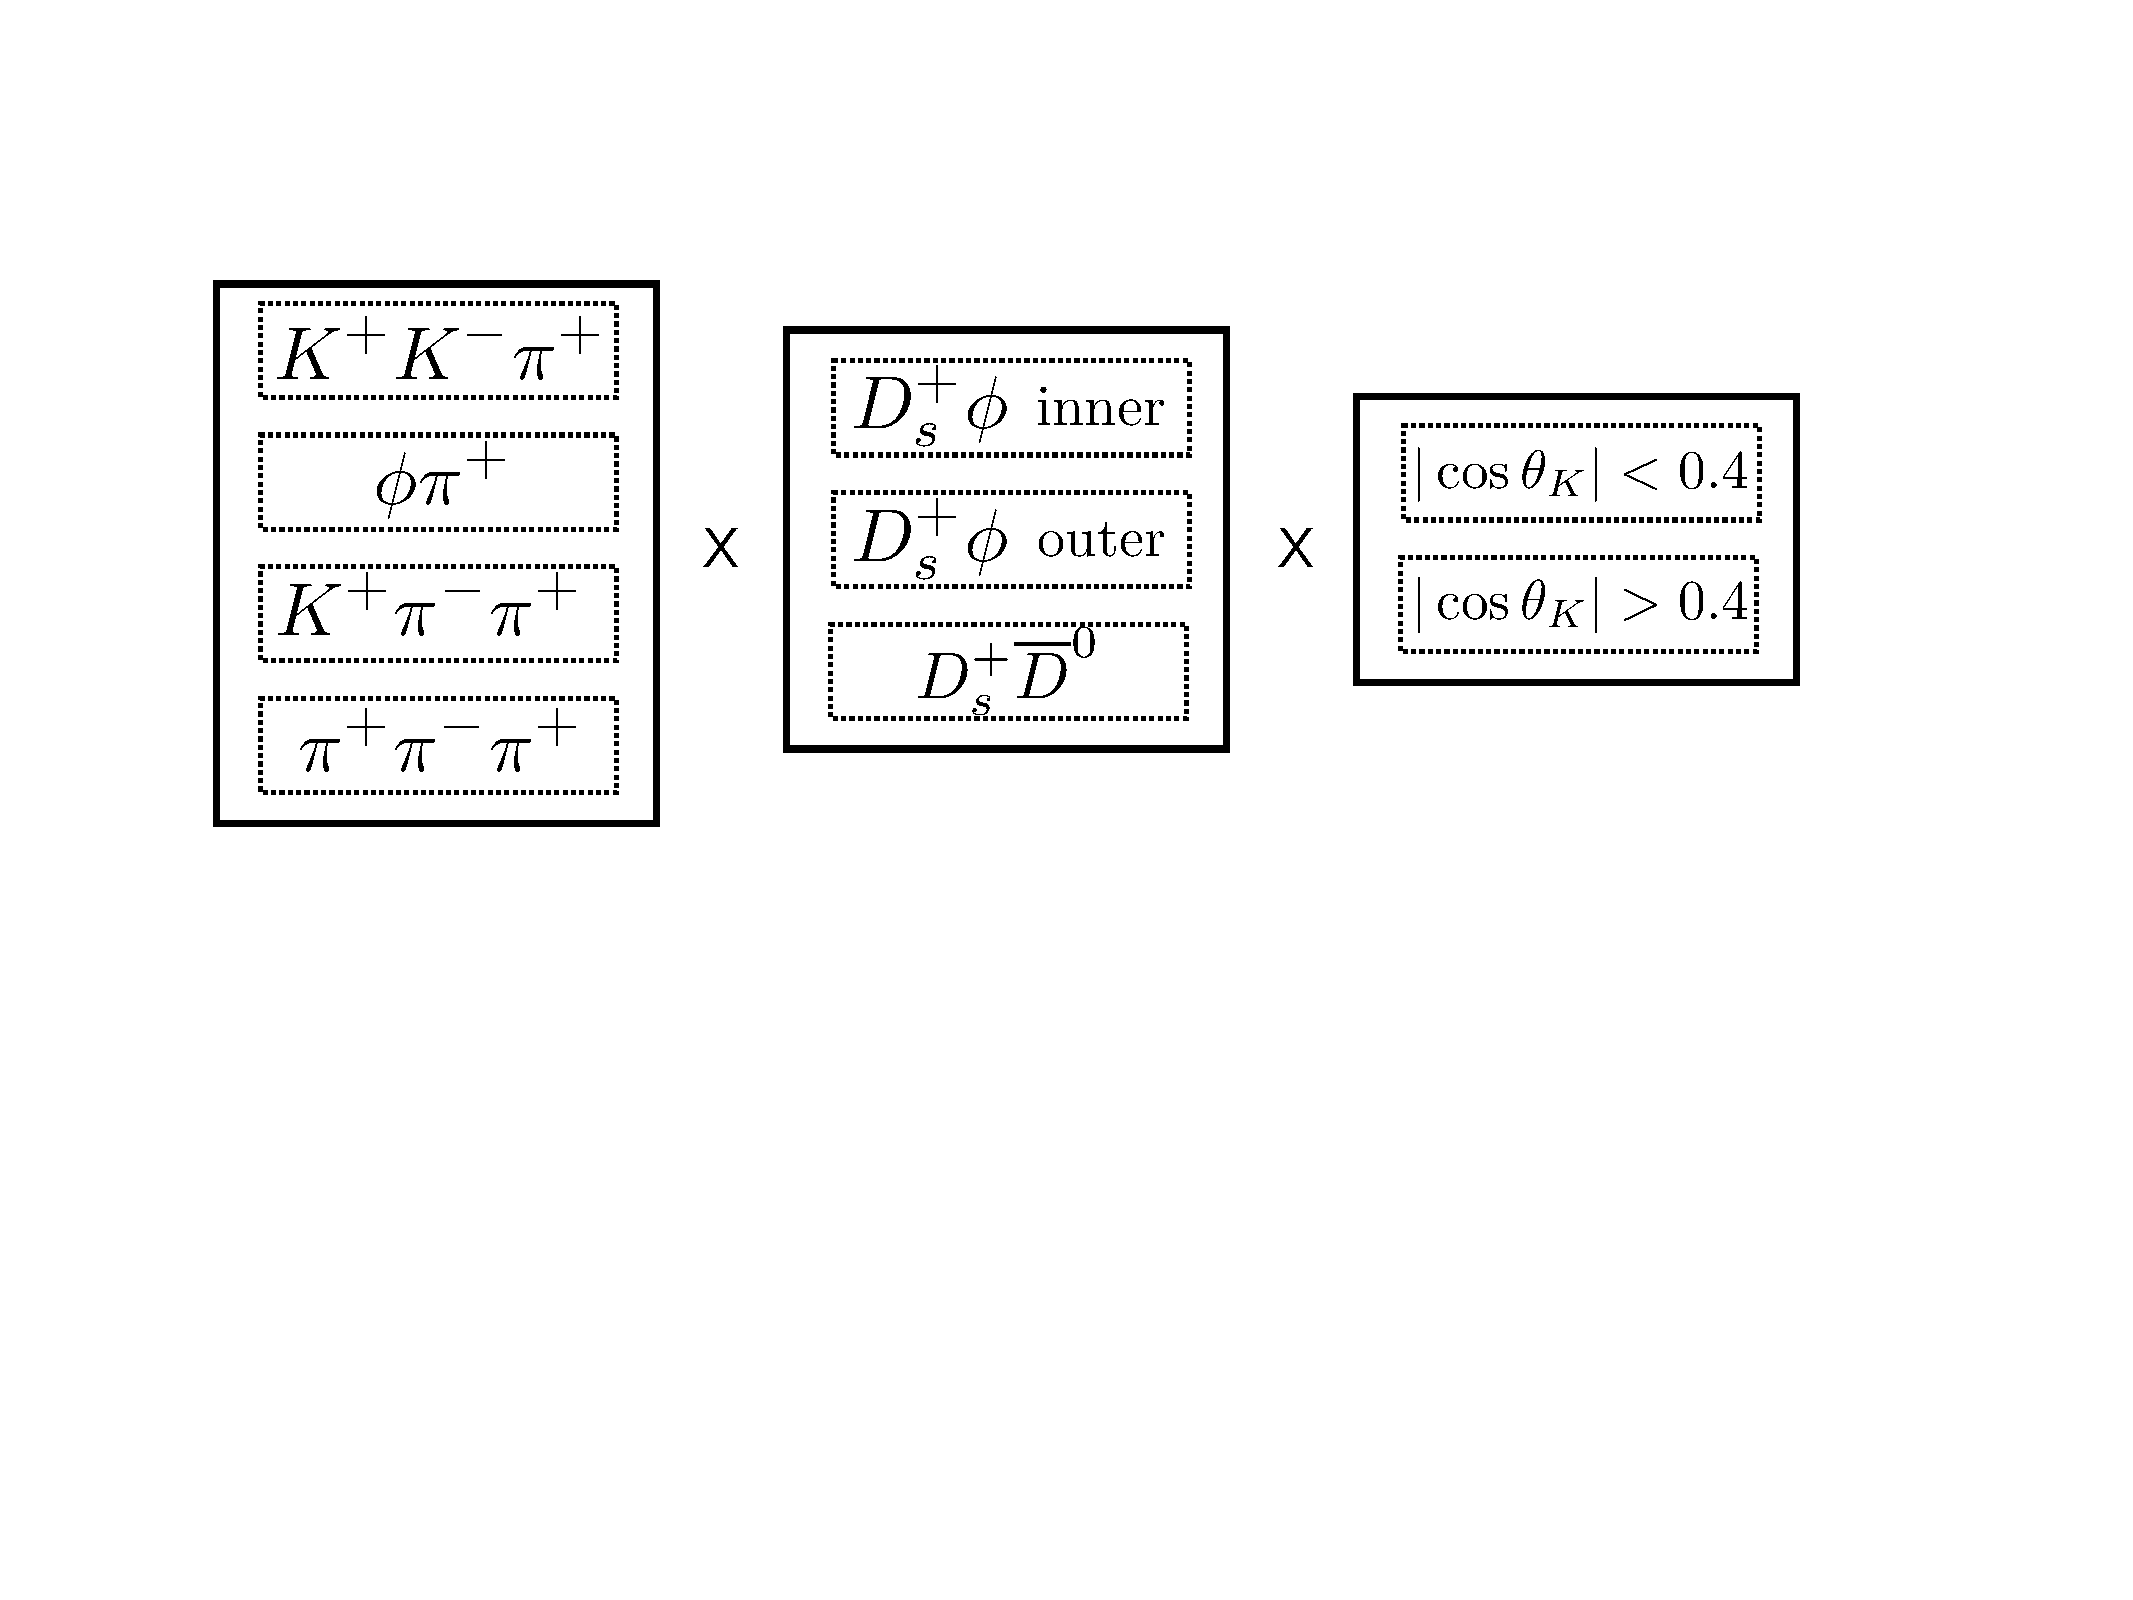
\includegraphics[width=0.7\textwidth]{figs/B2DsPhi/simfit_cats.pdf}
    \caption{The simultaneous fit categories include the \Dsp meson decay mode (left), invariant mass of the bachelor \Kp\Km pair (centre) and helicity angle (right).}
    \label{fig:B2DsPhi_simfit}   
\end{figure}
%%%%%%%%%%%%%%%%%%%%%%%%%%%%%%%%%%%%%%%%%%%%%%%%%%%%%%%%%%


\subsubsection{\Dsp meson decay mode} 
The three \Dsp decays modes used to reconstruct the signal and normalisation decays (\decay{\Dsp}{\Kp\Km\pip}, \decay{\Dsp}{\pip\pim\pip}, and \decay{\Dsp}{\Kp\pim\pip}) are fitted simultaneously in different categories. This allows the invariant mass distributions for the three modes to vary slightly in ways that could not be easily accounted for if the modes were combined in a single data set. In principle, the widths and resolutions of the \Bp meson mass distributions could vary for the three different modes as a result of the different numbers of pions and kaons in the final state. The background levels also differ between the modes as a result of the smaller branching fractions for \decay{\Dsp}{\pip\pim\pip} and \decay{\Dsp}{\Kp\pim\pip}. This leads to the background from combinations of unrelated tracks having a larger relative contribution.

The \decay{\Dsp}{\Kp\Km\pip} decay mode is additionally split into two further categories; candidates consistent with \decay{\Dsp}{\phiz\pip} decays, and those candidates from elsewhere in the \decay{\Dsp}{\Kp\Km\pip} Dalitz plane. This exploits the high purity of \decay{\Dsp}{\phiz\pip} decays. 

\subsubsection{Invariant mass of the bachelor \Kp\Km pair, $m(\Kp\Km)$} 
Three distinct ranges of $m(\Kp\Km)$ invariant mass are used to split the candidates. The first of these corresponds to normalisation \decay{\Bp}{\Dsp\Dzb} candidates within the range $|m(\Kp\Km)-m(\Dzb)|<25 \mevcc$. The second corresponds to \decay{\Bp}{\Dsp\phiz} decays and is split into two ranges; those within $|m(\Kp\Km)-m(\phiz)|<10\mevcc$, referred to as the \emph{inner \phiz mass category} and those candidates with $10<|m(\Kp\Km)-m(\phiz)|<40\mevcc$, referred to as the \emph{outer \phiz mass category}. These two categories for the signal mode allow contributions from decays that do not proceed via a \phiz meson to be distinguished from those that do. The \emph{inner \phiz mass category} contains 88\% of signal \decay{\Bp}{\Dsp\phiz} candidates, with the other 12\% in the \emph{outer \phiz mass category}. The $m(\Kp\Km)$ invariant mass distribution for simulated \decay{\Bp}{\Dsp\phiz} is shown in Fig~\ref{fig:B2DsPhi_hel_mass_MC}.



%%%%%%%%%%%%%%%%%%%%%%%%%%%%%%%%%%%%%%%%%%%%%%%%%%%%%%%%%%
\begin{figure}[!h]
    \centering
    \begin{subfigure}[t]{0.48\textwidth}
        \centering
        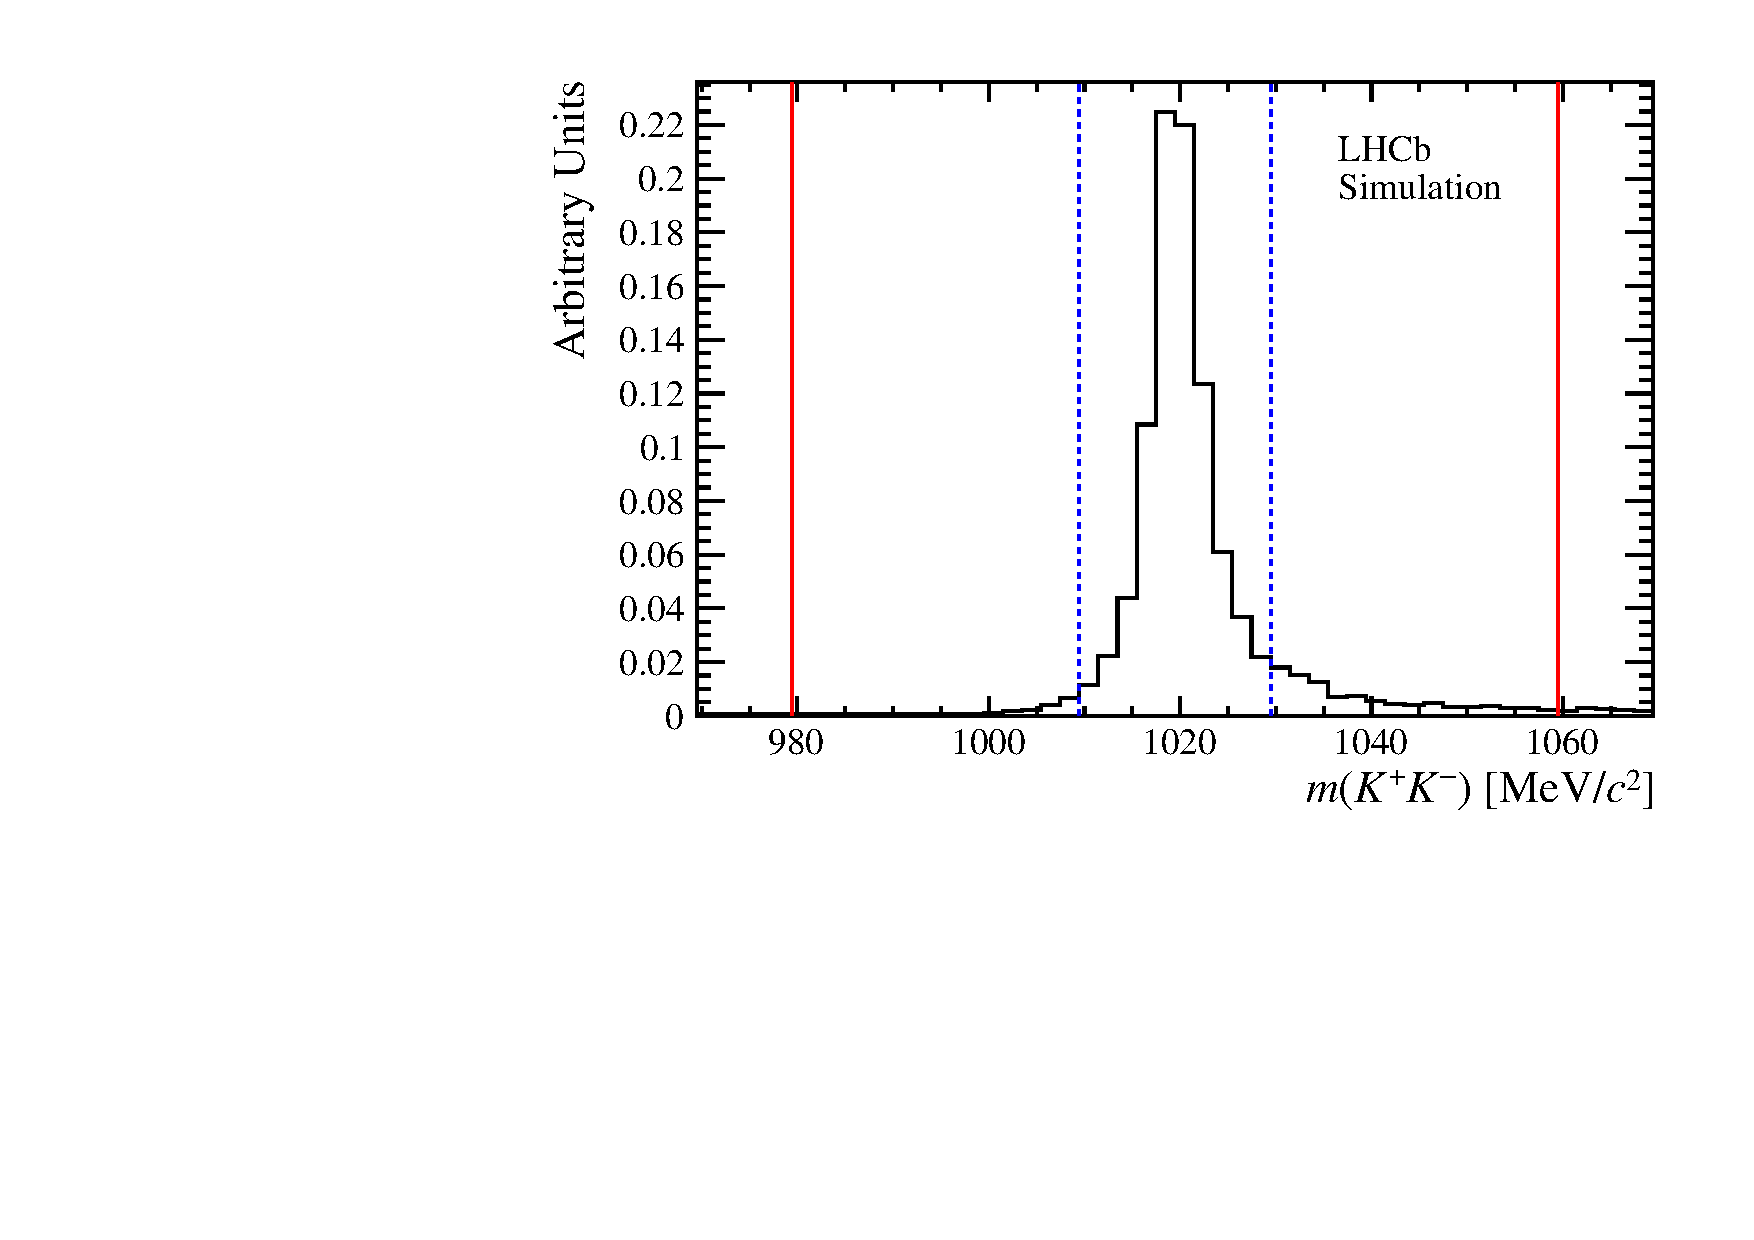
\includegraphics[width=1.0\textwidth]{figs/B2DsPhi/MC_Distributions_mass_B2DsPhi.pdf}
    \end{subfigure}
    \begin{subfigure}[t]{0.48\textwidth}
        \centering
        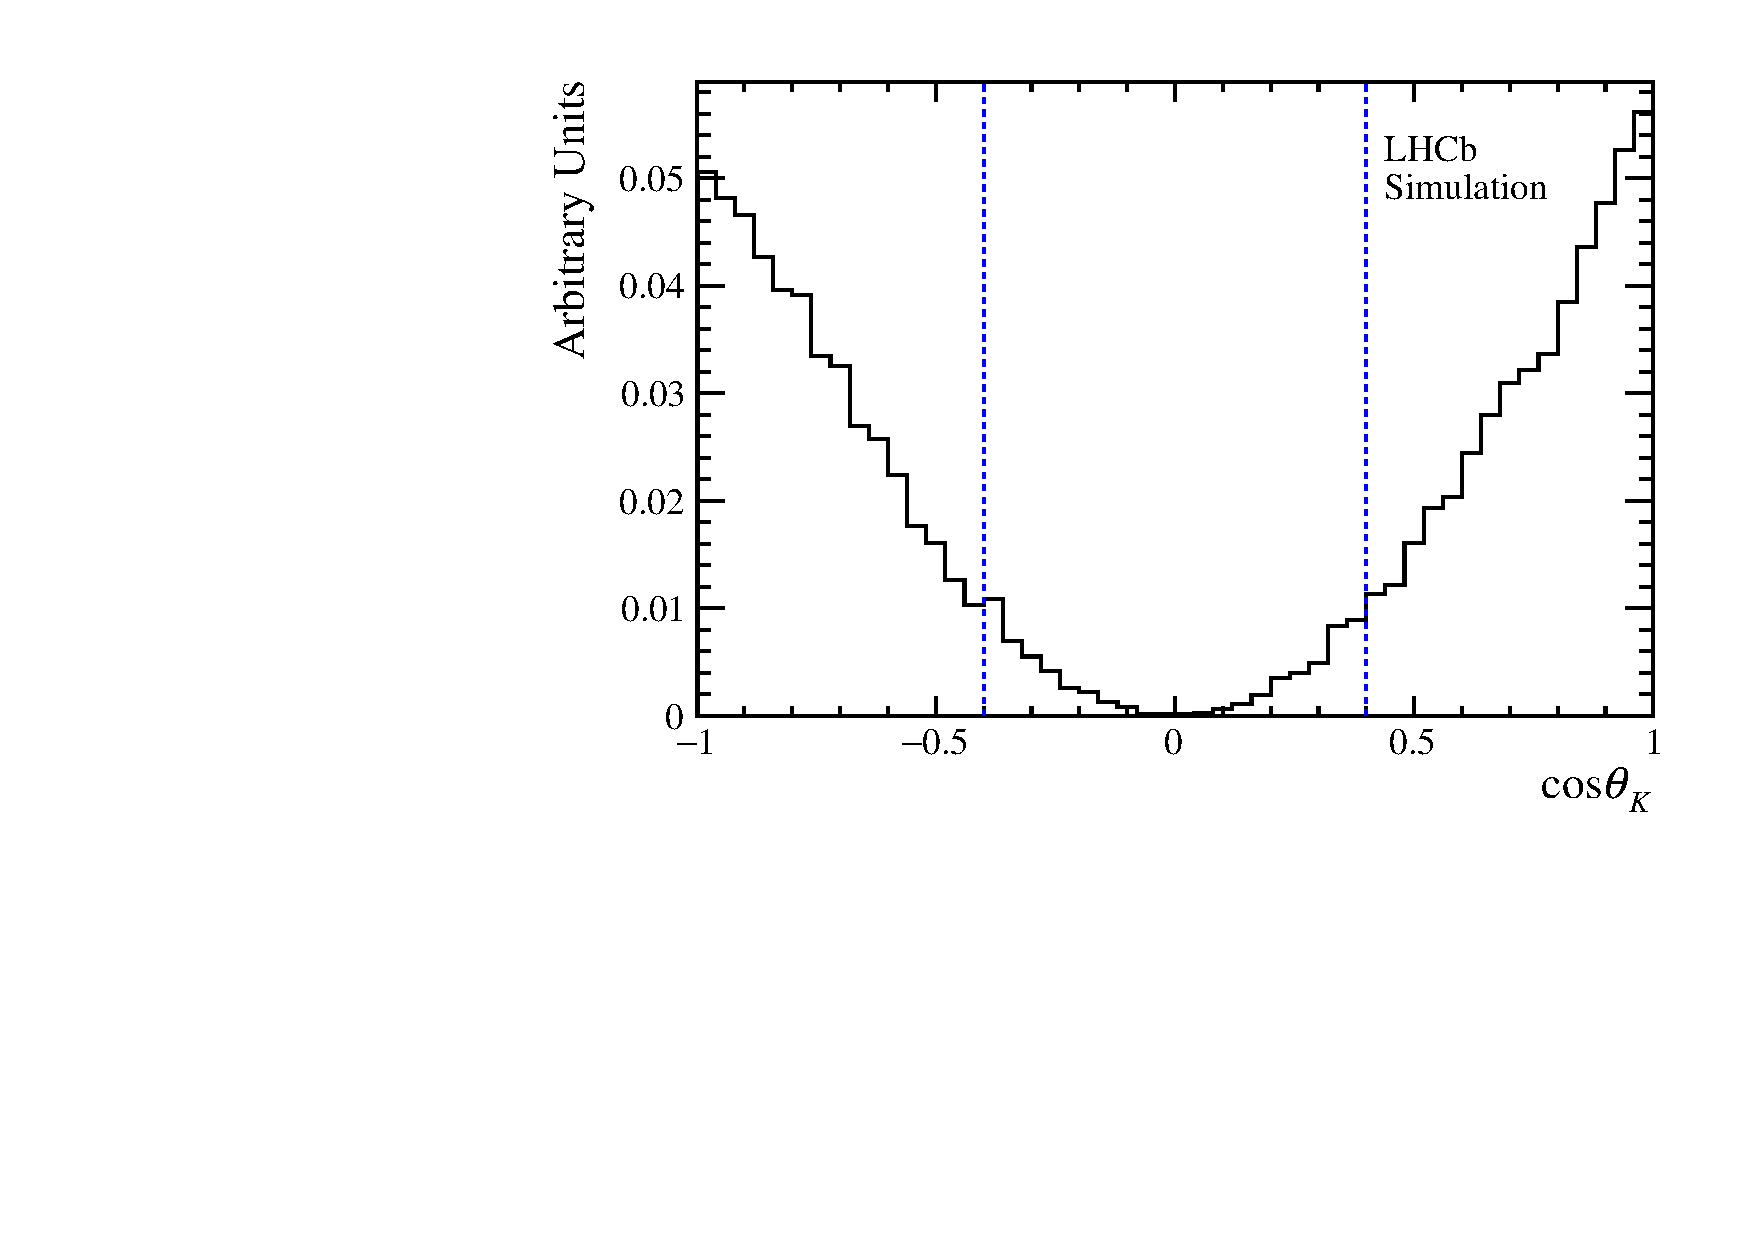
\includegraphics[width=1.0\textwidth]{figs/B2DsPhi/MC_Distributions_angle_B2DsPhi.pdf}
    \end{subfigure}
    \caption{The distributions of $m(\Kp\Km)$ (left) and $\cos\theta_{K}$ (right) in simulated \decay{\Bp}{\Dsp\phiz} decays. The vertical blue dashed lines represent the boundaries between categories defined in Sec.~\ref{sec:B2DsPhi_fit_cats}. The vertical red lines represent the mass window applied to candidates; those outside the red lines are not included in the data set.}
    \label{fig:B2DsPhi_hel_mass_MC}   
\end{figure}
%%%%%%%%%%%%%%%%%%%%%%%%%%%%%%%%%%%%%%%%%%%%%%%%%%%%%%%%%%


%MC_Distributions_mass_B2DsPhi.pdf



\subsubsection{Helicity angle, $\cos\theta_{K}$} 

The $\decay{\Bp}{\Dsp\phiz}$ decay involves the decay of a pseudoscalar particle (\Bp) to a pseudoscalar (\Dsp) and vector particle (\phiz), $\decay{0^{-}}{0^{-}1^{-}}$. In general, spin-1 \phiz mesons can be in $\lambda= +1,0,-1$ polarisation states. However, to conserve angular momentum in \decay{\Bp}{\Dsp\phiz} decays it must be produced in the $\lambda = 0$ state. 
%To conserve angular momentum, the \Dsp\phiz system must be produced in a $J ^{P} = 0^{-}$ state. This is only possible if the $z$-component of the \phiz meson's total angular momentum is $J_{z} = 0$, hence it is produced longitudinally polarised.
%Therefore the \phiz vector meson ($J^{P} = 1^{-}$) must be produced longitudinally polarised. 

The decay  \decay{\phiz}{\Kp\Km} is a $\decay{1^{-}}{0^{-}0^{-}}$ process. 
The distribution of the angle $\theta_{K}$, defined as the angle that the kaon meson forms with the \Bp momentum in the \phiz rest frame (Fig.~\ref{fig:B2DsPhi_helicity_angle}) depends on the polarisation state of the \phiz meson. For \phiz mesons in the $\lambda = 0$ ($\lambda = \pm1$) polarisation state this is proportional to $\cos^{2}{\theta_{K}}$ ($\sin^{2}{\theta_{K}}$).


%To conserve angular momentum, the decay products must be produced with a relative orbital angular momentum of $L_{r} = 1$. 
%For a longitudinally polarised \phiz meson decaying to $\Kp\Km$, 
%The distribution of the angle $\theta_{K}$, defined as the angle that the kaon meson forms with the \Bp momentum in the \phiz rest frame (Fig.~\ref{fig:B2DsPhi_helicity_angle}), is proportional to $\cos^{2}{\theta_{K}}$. 

The distribution of $\cos{\theta_{K}}$ for $\decay{\Bp}{\Dsp\phiz}$ as determined from simulated events is shown in Fig~\ref{fig:B2DsPhi_hel_mass_MC}. Candidates are split into two categories chosen to help separate the signal from other decays; $|\cos{\theta_{K}} |> 0.4$ and $|\cos{\theta_{K}} |< 0.4$. These categories contain 93\% and 7\% of the signal respectively.
%%%%%%%%%%%%%%%%%%%%%%%%%%%%%%%%%%%%%%%%%%%%%%%%%%%%%%%%%%
\begin{figure}[!h]
    \centering
    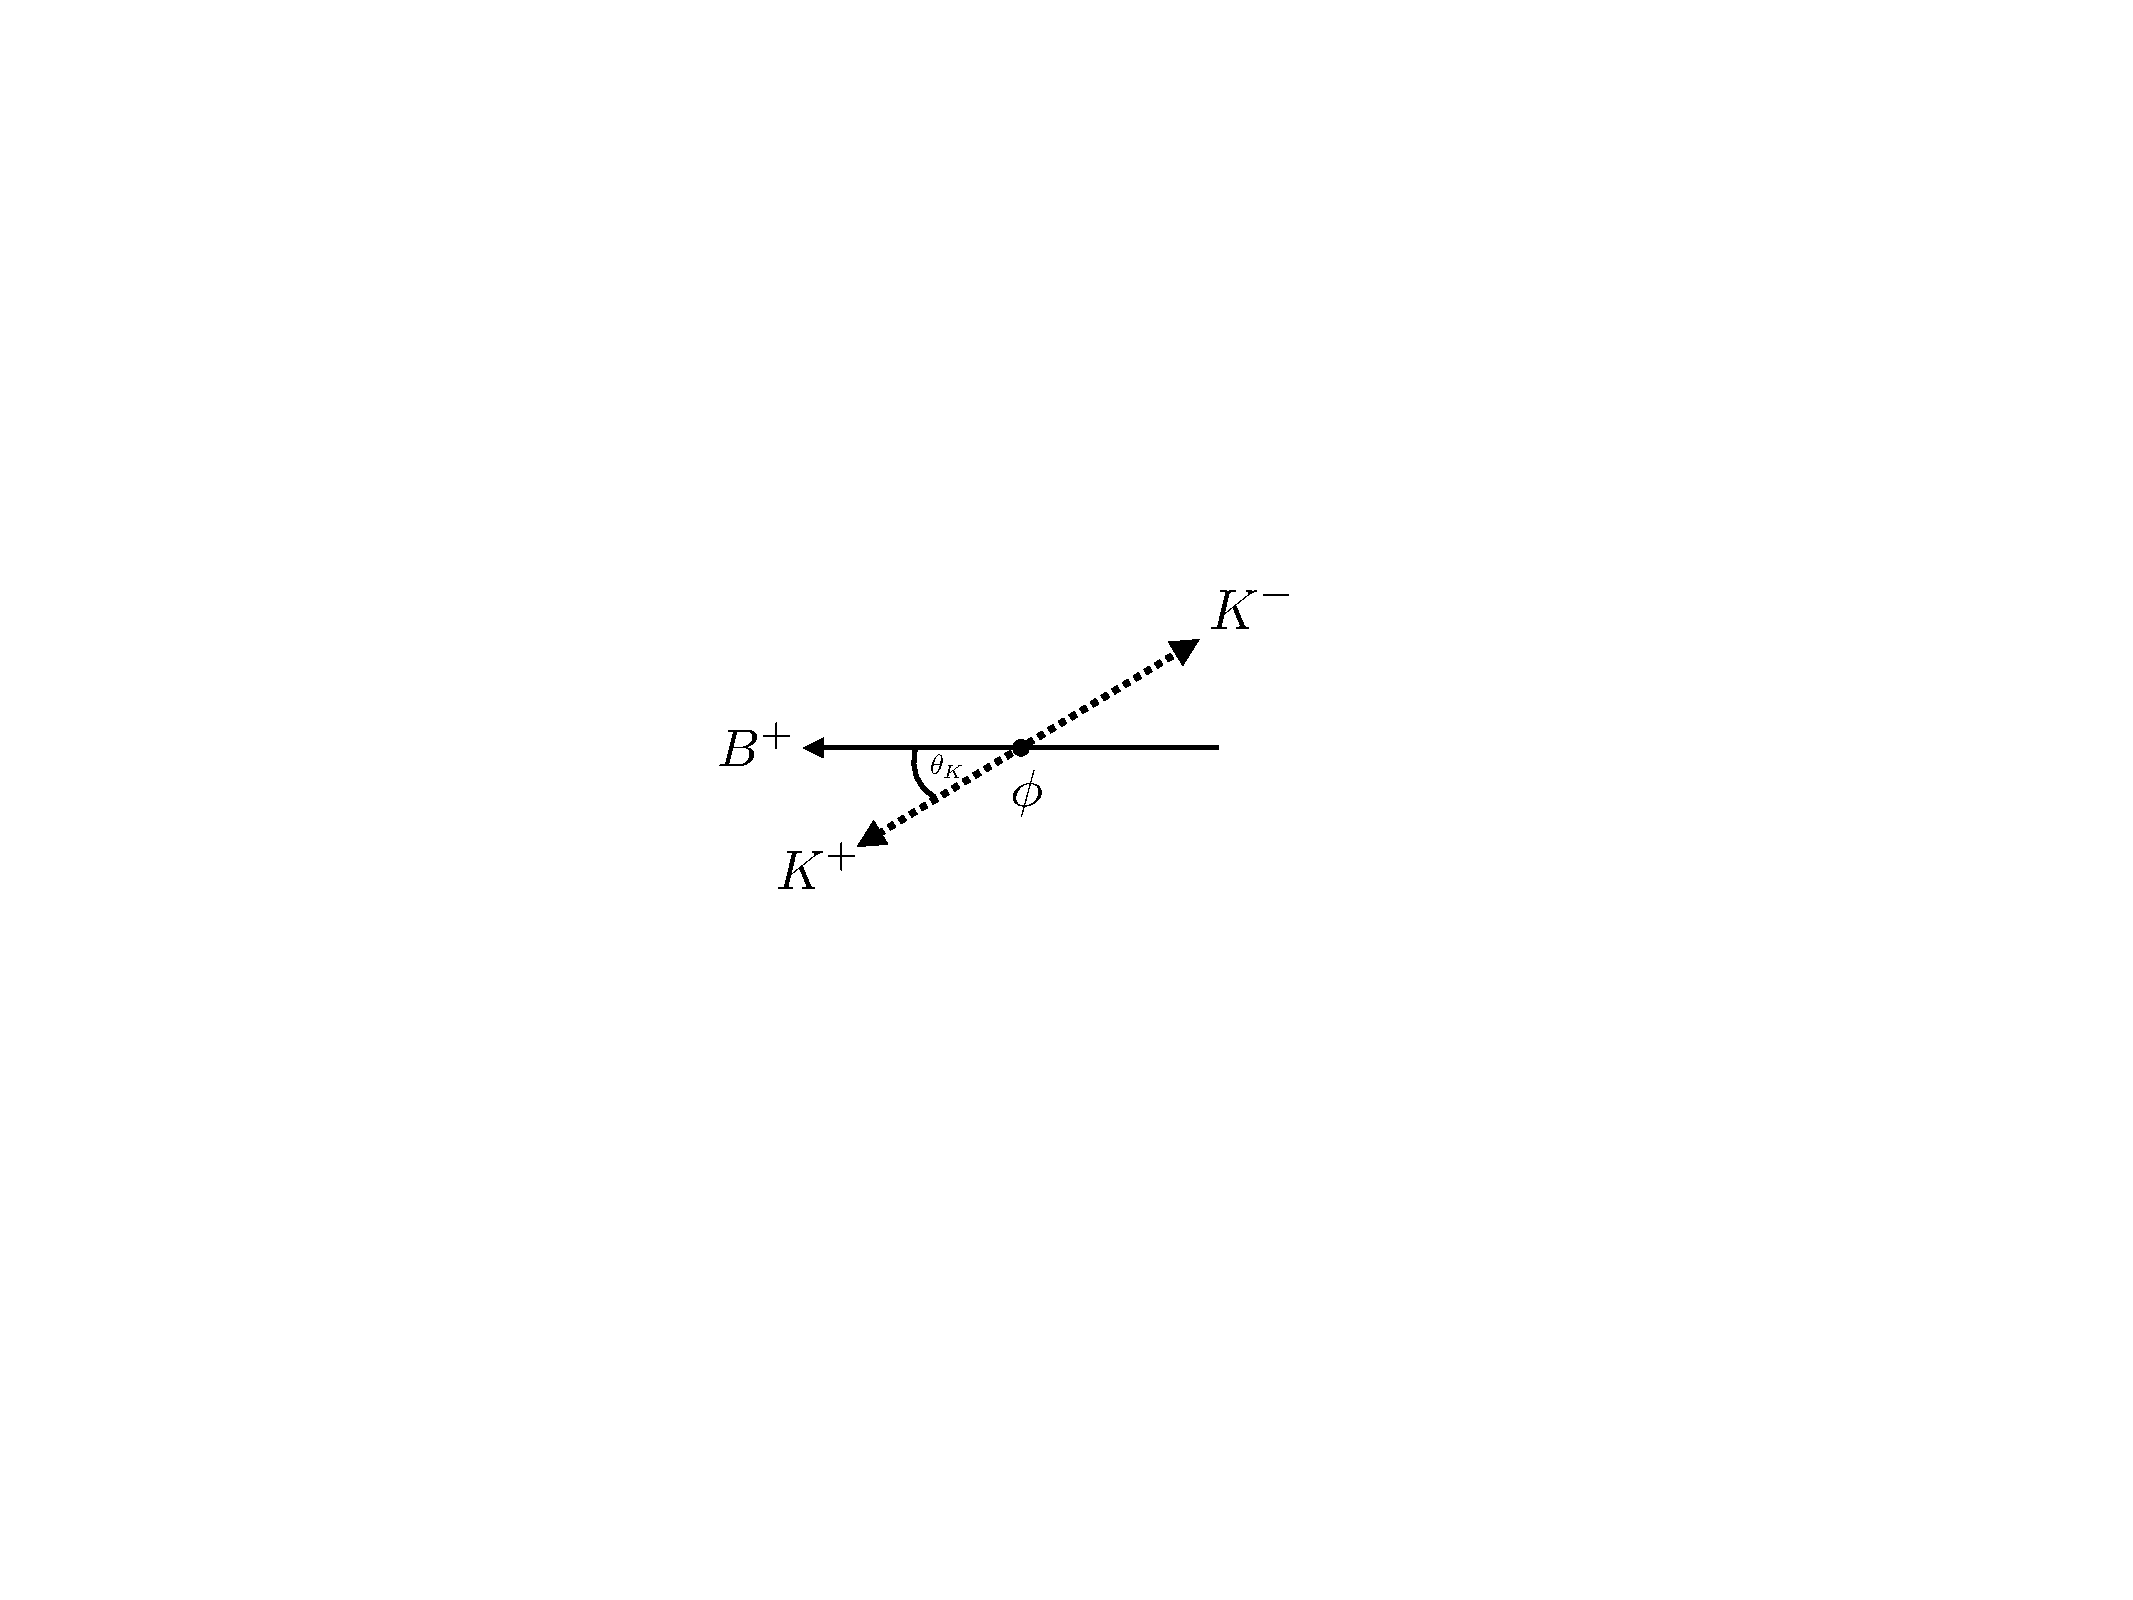
\includegraphics[width=0.48\textwidth]{figs/B2DsPhi/helicityangle.pdf}
    \caption{The angle $\theta_{K}$ (referred to as the helicity angle) is defined to be the angle that the kaon mesons forms with the \Bp meson momentum in the \phiz rest frame.}
    \label{fig:B2DsPhi_helicity_angle}   
\end{figure}
%%%%%%%%%%%%%%%%%%%%%%%%%%%%%%%%%%%%%%%%%%%%%%%%%%%%%%%%%%

This helicity angle is constructed using the momentum of the decay products calculated after the whole decay chain has been refitted with a \Dsp mass and \Bp direction constraint. 


\begin{table}[t]
   \centering
   \begin{tabular}{c|cc}
      \hline
      \multirow{2}{*}{$| m(\Kp\Km) - m_{\phi} |$ (\mevcc)}   & \multicolumn{2}{c}{Helicity Category} \\ 
                       & $|\cos{\theta_{K}} |> 0.4$          & $|\cos{\theta_{K}} |< 0.4$\\ 
      \hline
      $< 10$                           & 82\%           & 6\%                       \\
      (10, 40)                         & 11\%           & 1\%                       \\
      \hline
  \end{tabular}
  \caption{Fractions of $\decay{\Bp}{\Dsp\phiz}$ candidates expected in the helicity and $m(\Kp\Km)$ invariant mass categories of the simultaneous fit. }
  \label{tab:signal_ratios}
\end{table}


\subsection{\decay{\Bp}{\Dsp \Kp \Km} model and assumptions}
\label{sec:B2DsPhi_B2DsKKModel}
The search for \decay{\Bp}{\Dsp\phiz} decays includes a component for \decay{\Bp}{\Dsp\Kp\Km} decays that do not proceed via a \phiz meson. To avoid overestimating \decay{\Bp}{\Dsp\phiz} signal yield, separate components are included in the fit model for the \decay{\Bp}{\Dsp\phiz} and \decay{\Bp}{\Dsp\Kp\Km} decays. Although the invariant mass PDFs of these two contributions are identical, they can still be disentangled by exploiting the different fractions of these decays expected in each of the helicity angle and $m(\Kp\Km)$ categories: \decay{\Bp}{\Dsp\phiz} decays peak sharply in $m(\Kp\Km)$ whilst \decay{\Bp}{\Dsp\Kp\Km} are flat; and \decay{\Bp}{\Dsp\phiz} decays peak sharply around $\cos{\theta_{K}} = \pm 1$ whilst \decay{\Bp}{\Dsp\Kp\Km} doesn't necessarily. 


The fractions for the \decay{\Bp}{\Dsp\phiz} signal decays as listed in Table~\ref{tab:signal_ratios} show the decays are concentrated in the \emph{inner \phiz mass category} with $|\cos{\theta_{K}} |> 0.4$. 


% To determine similar fractions for \decay{\Bp}{\Dsp\Kp\Km} decays the \laurapp package~\cite{1711.09854} is used to generate a number of simulation samples for different intermediate resonance models.

% Only resonances in the \Kp\Km system are considered as no significant structure is observed in the $m(\Dsp\Km)$ distribution in Fig.~\ref{fig:B2DsKK_twobodyprojections}. As such, all resonances are neutral mesons. The models are generated separately, therefore the effect of interference between any combination of states has been entirely neglected.    
% The generated samples are described in the following sections.

% \subsubsection{The $\phi(1020)$ resonance} 
% Decays proceeding via a $\phiz(1020)$ are produced as a crosscheck. As the simulations generated with \laurapp have not been reconstructed with the full \lhcb detector model, this sample is compared to the existing full simulation samples. The differences in between the fraction of the decays in the different $m(\Kp\Km)$ and $\cos\theta_{K}$ categories in the two samples are taken as a proxy for the potential level of bias introduced by using these generator level samples instead of full simulation. The distribution of these simulated decays in $m(\Kp\Km)$ and $\cos\theta_{K}$ are shown in Fig.~\ref{fig:DsKK_model_phi1020}. This figure also include the Dalitz plot distribution of the decays parametrised with the variables $m^{2}(\Dsp\Km)$ and $m^{2}(\Kp\Km)$.
% This resonance is generated with a Relativistic Breit-Wigner line shape~\cite{RelBWPhysRev.49.519}.
% %%%%%%%%%%%%%
% \begin{figure}[!h]
%    \centering   
%    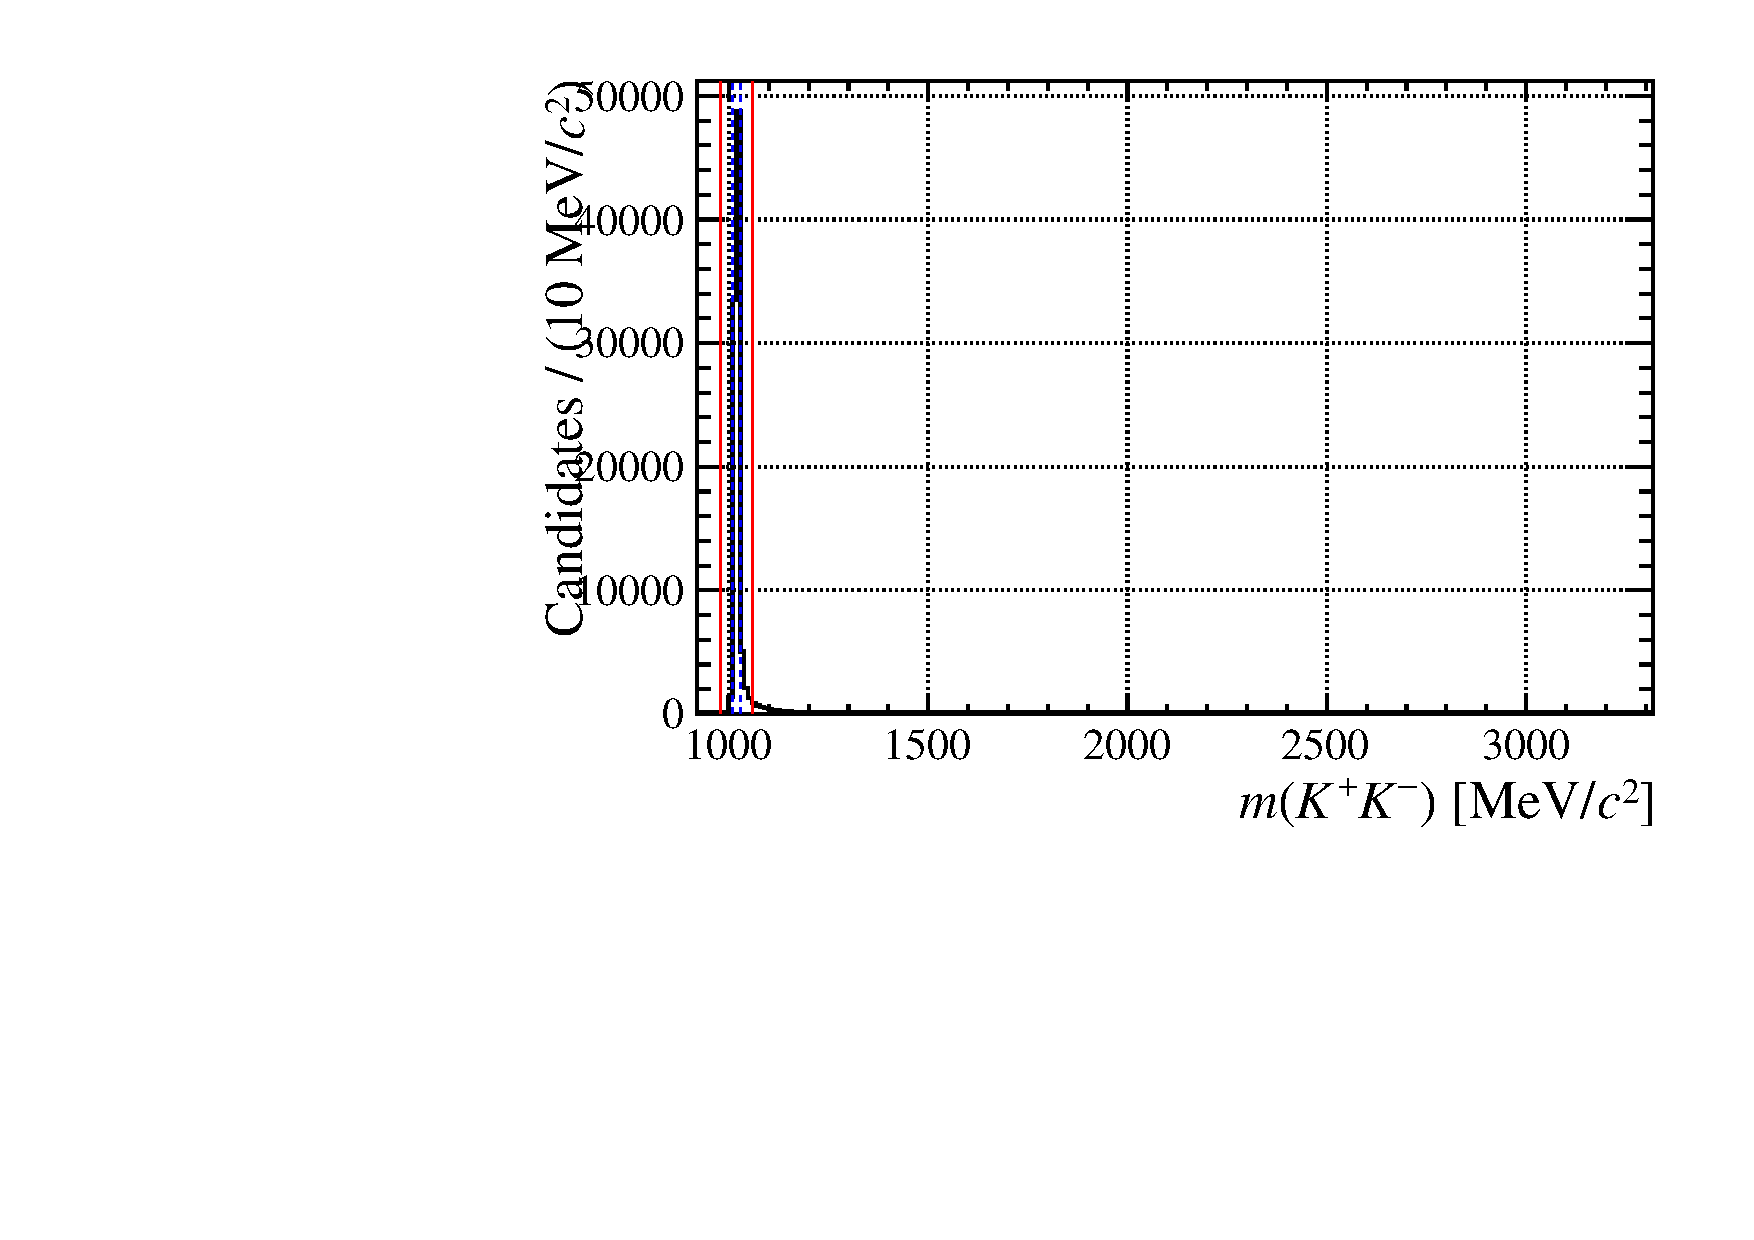
\includegraphics[width=0.32\textwidth]{figs/B2DsPhi/phi_phi_mass.pdf}
%    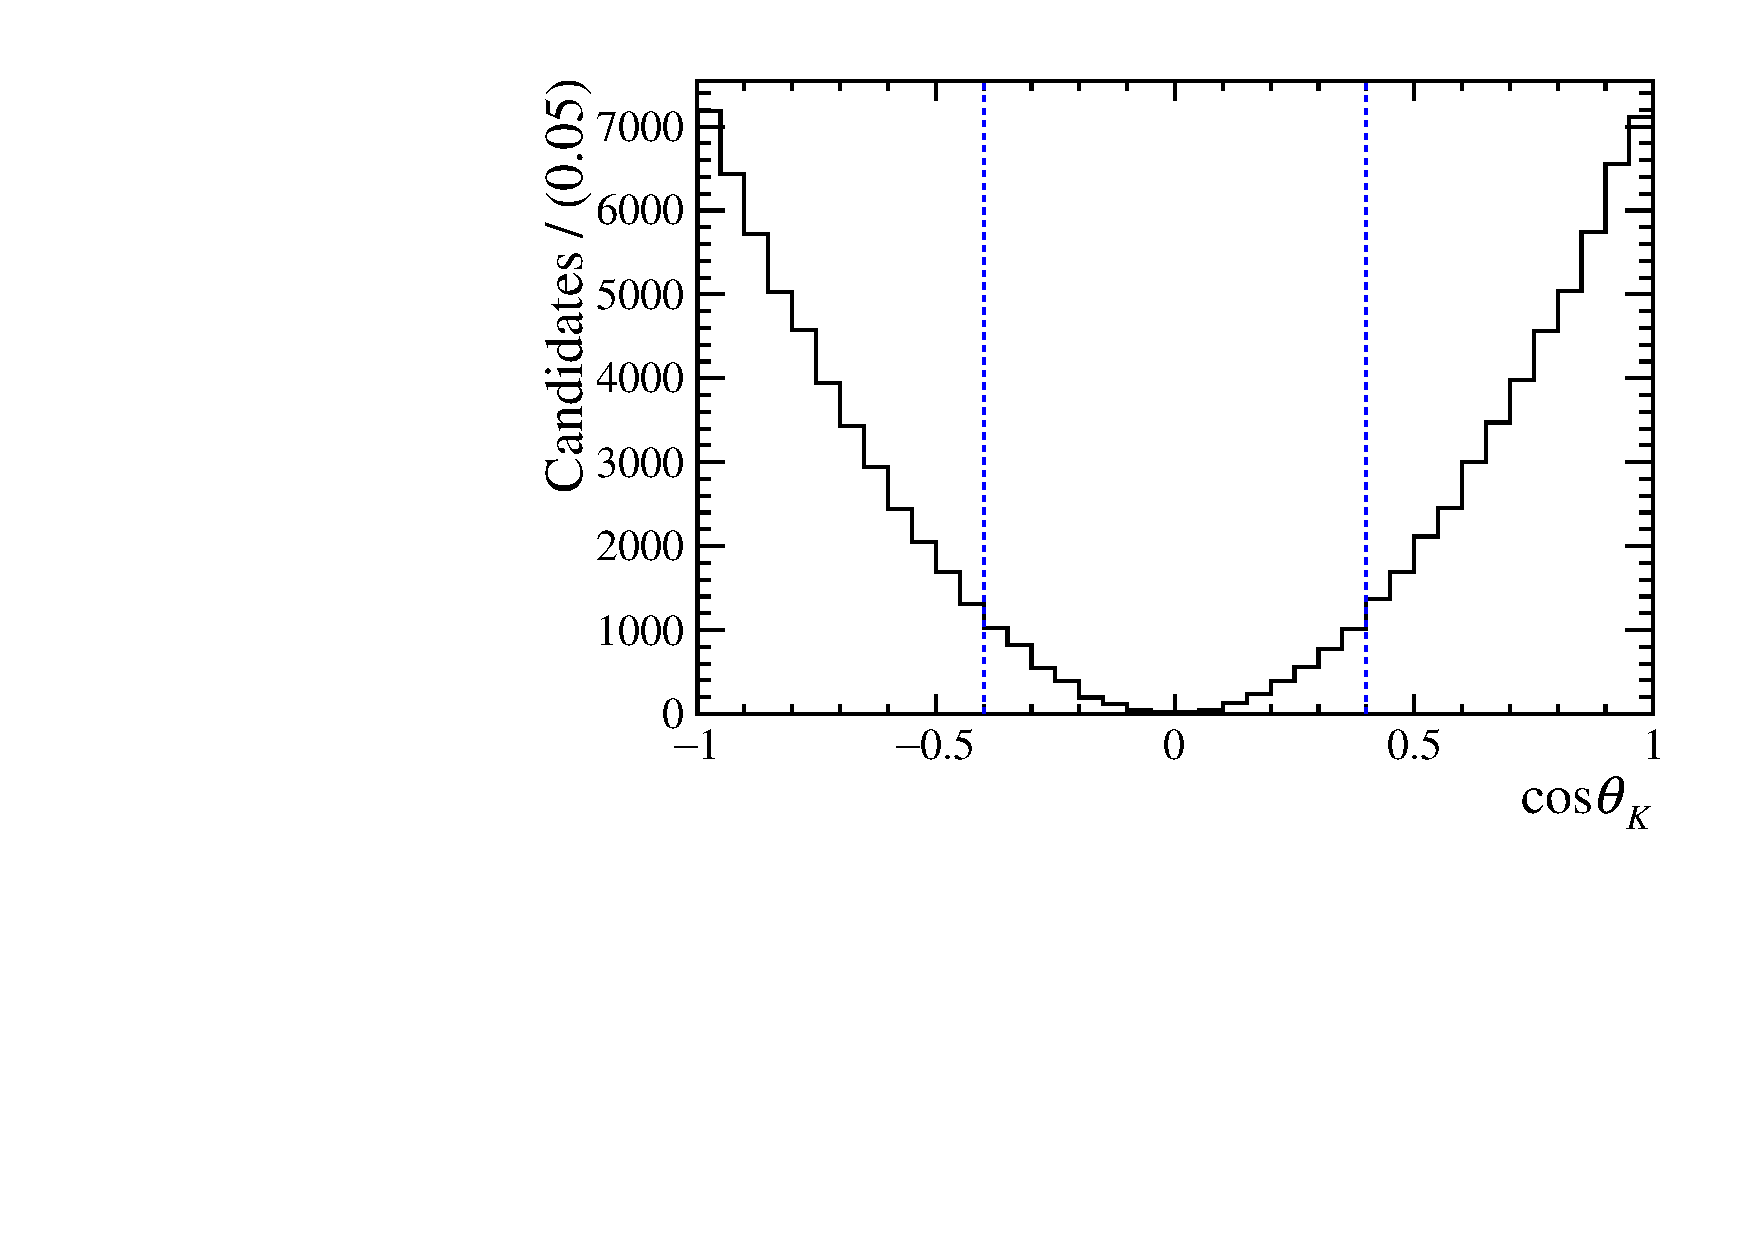
\includegraphics[width=0.32\textwidth]{figs/B2DsPhi/phi_Helicity.pdf}
%    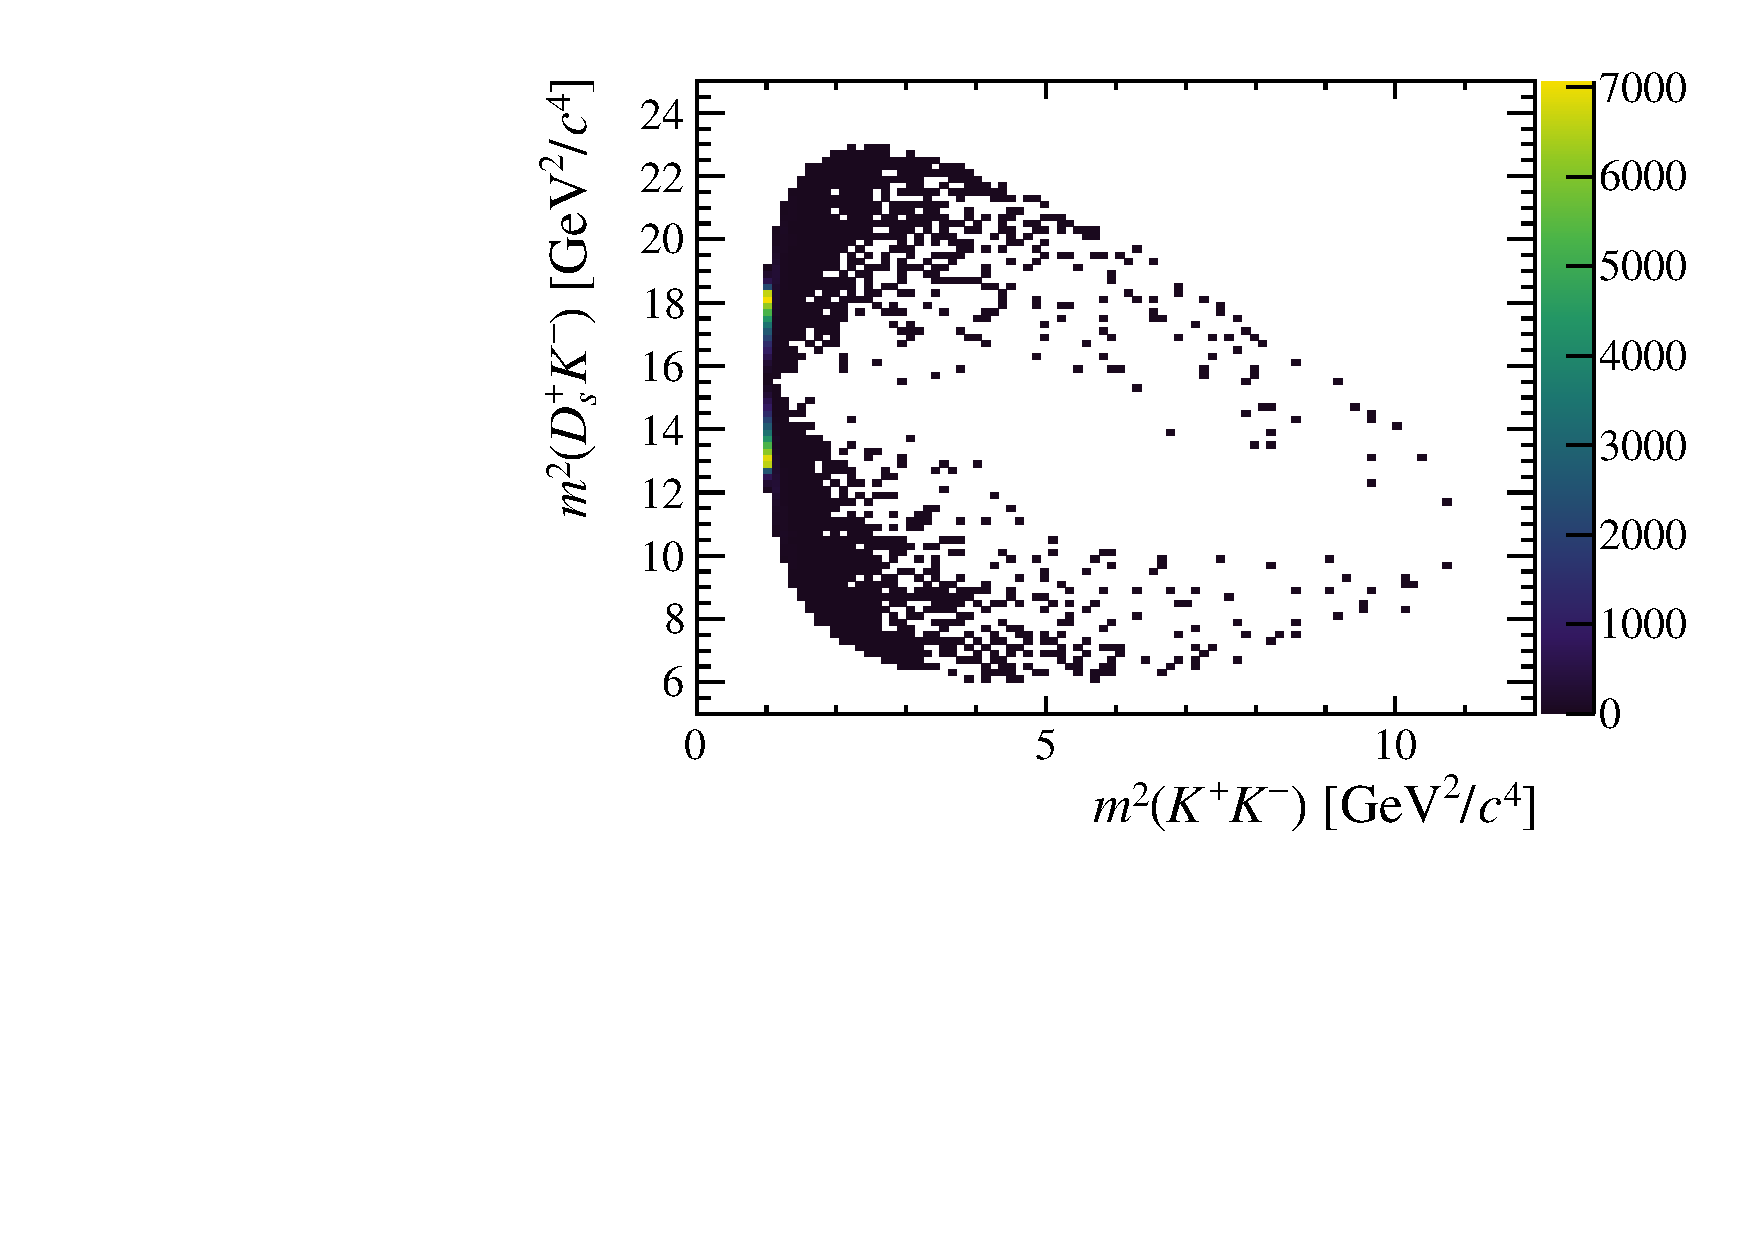
\includegraphics[width=0.32\textwidth]{figs/B2DsPhi/phi_Dalitz_plot.pdf}
%    \caption{The distribution of $m(\Kp\Km)$ (left), Dalitz plot (middle) and the helicity angle $\cos\theta_{K}$ for generated for the $\phiz(1020)$ resonance.} 
%    \label{fig:DsKK_model_phi1020}   
% \end{figure}
% %%%%%%%%%%%%%

% \subsubsection{Non-resonant decays}

% In addition to \Kp\Km resonances, a non-resonant model is considered. This model is defined to have a uniform amplitude across the allowed phase-space. The distribution in $m(\Kp\Km)$ of \decay{\Bp}{\Dsp\Kp\Km} decays in Fig.~\ref{fig:B2DsKK_twobodyprojections} is not consistent with this model as there are no candidates above $m(\Kp\Km) \sim 1900\mevcc$. However, this component is included in this study for comparative purposes. The distributions of decays generated with this flat model are shown in Fig.~\ref{fig:DsKK_model_NR}. 

% %%%%%%%%%%%%%
% \begin{figure}[!h]
%    \centering   
%    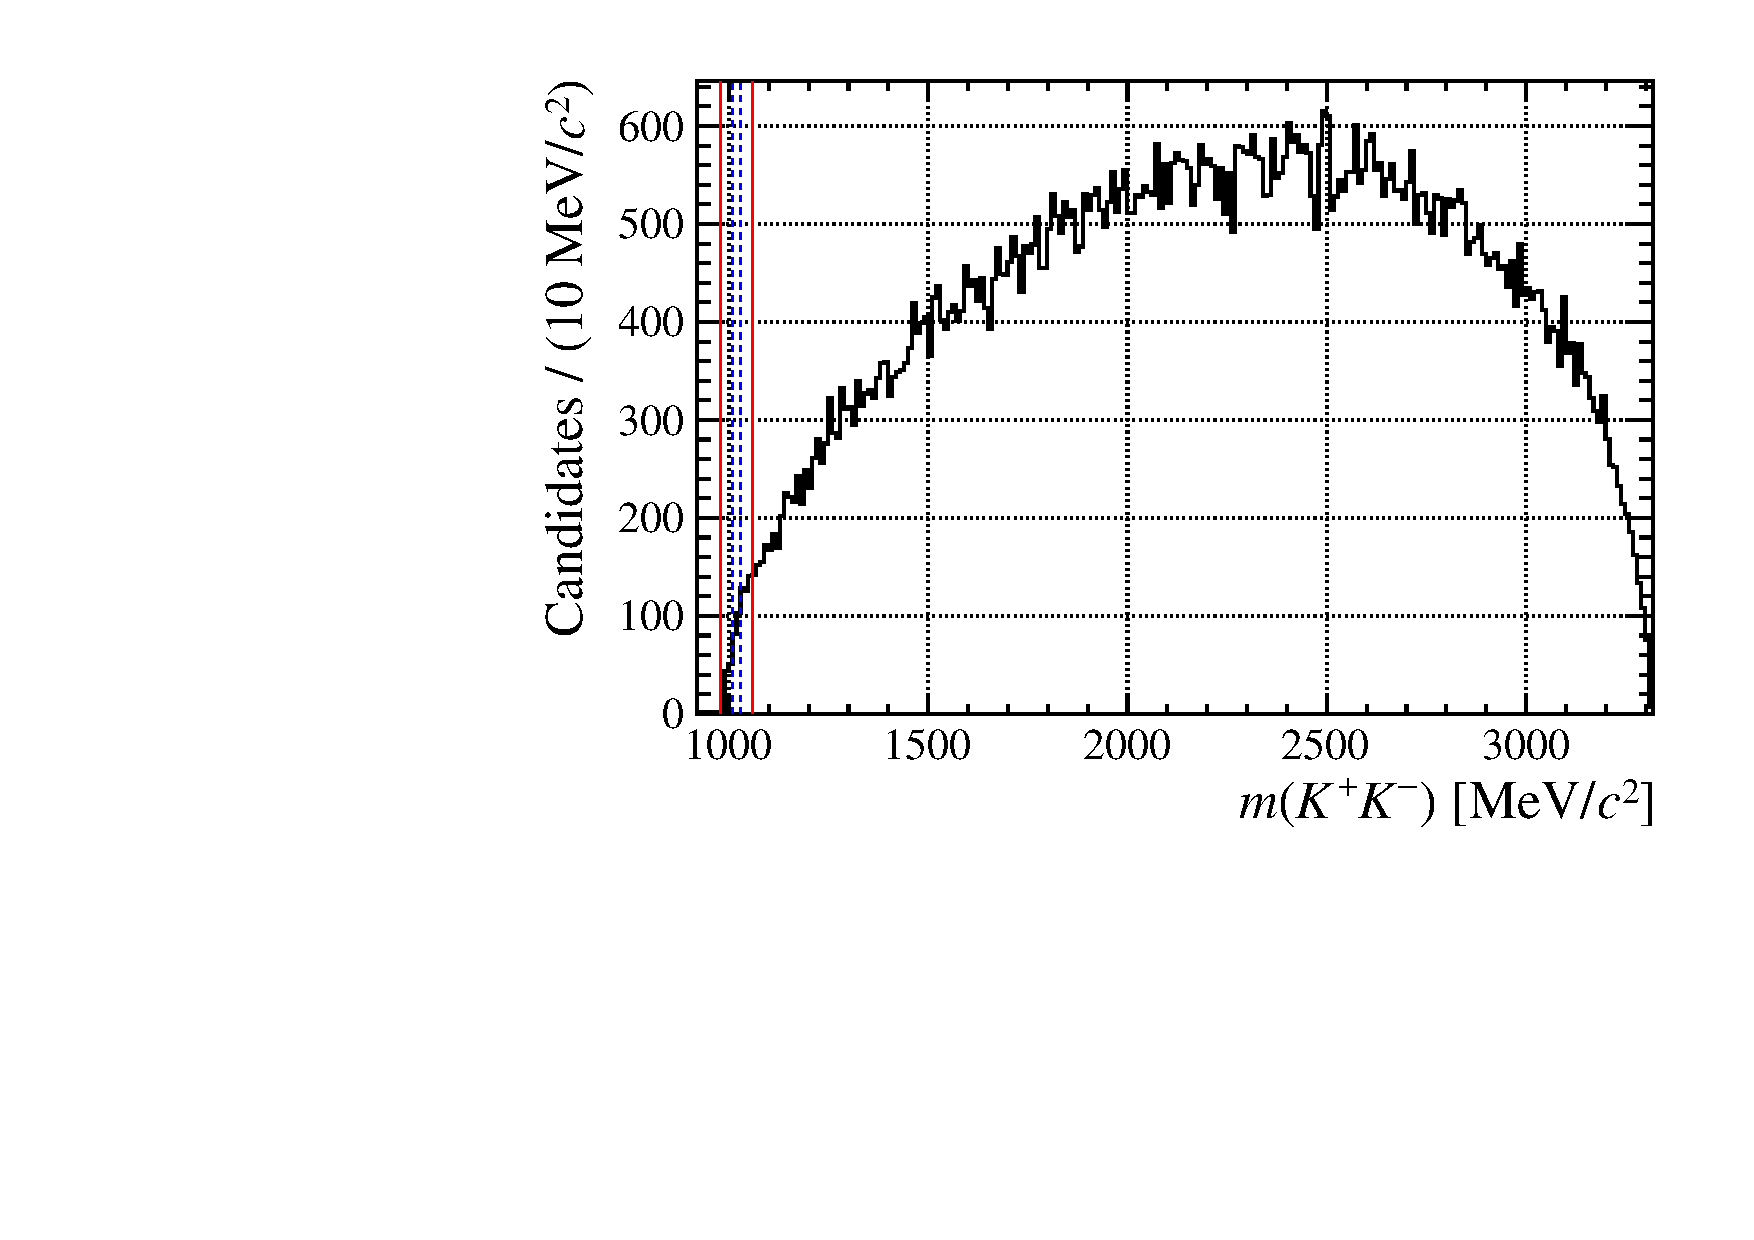
\includegraphics[width=0.32\textwidth]{figs/B2DsPhi/NR_phi_mass.pdf}
%    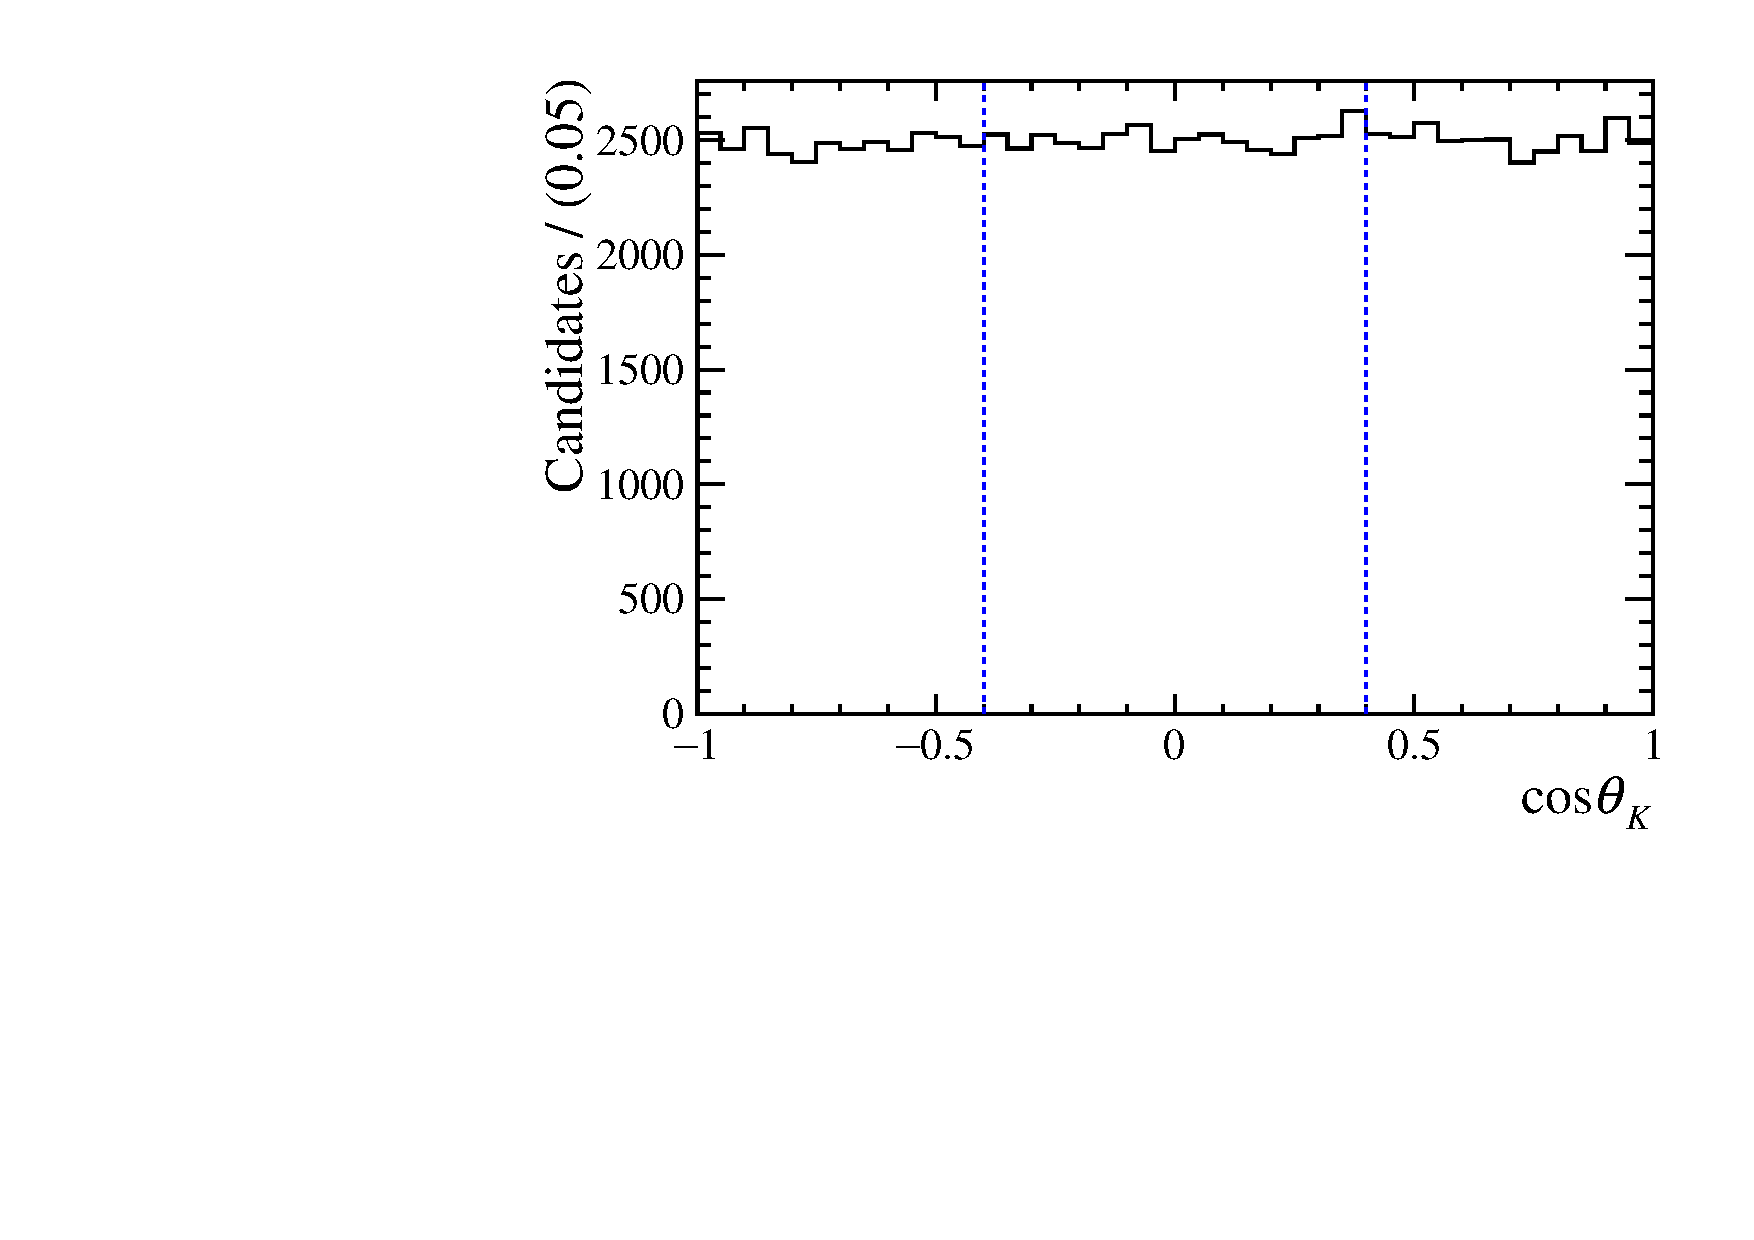
\includegraphics[width=0.32\textwidth]{figs/B2DsPhi/NR_Helicity.pdf}
%    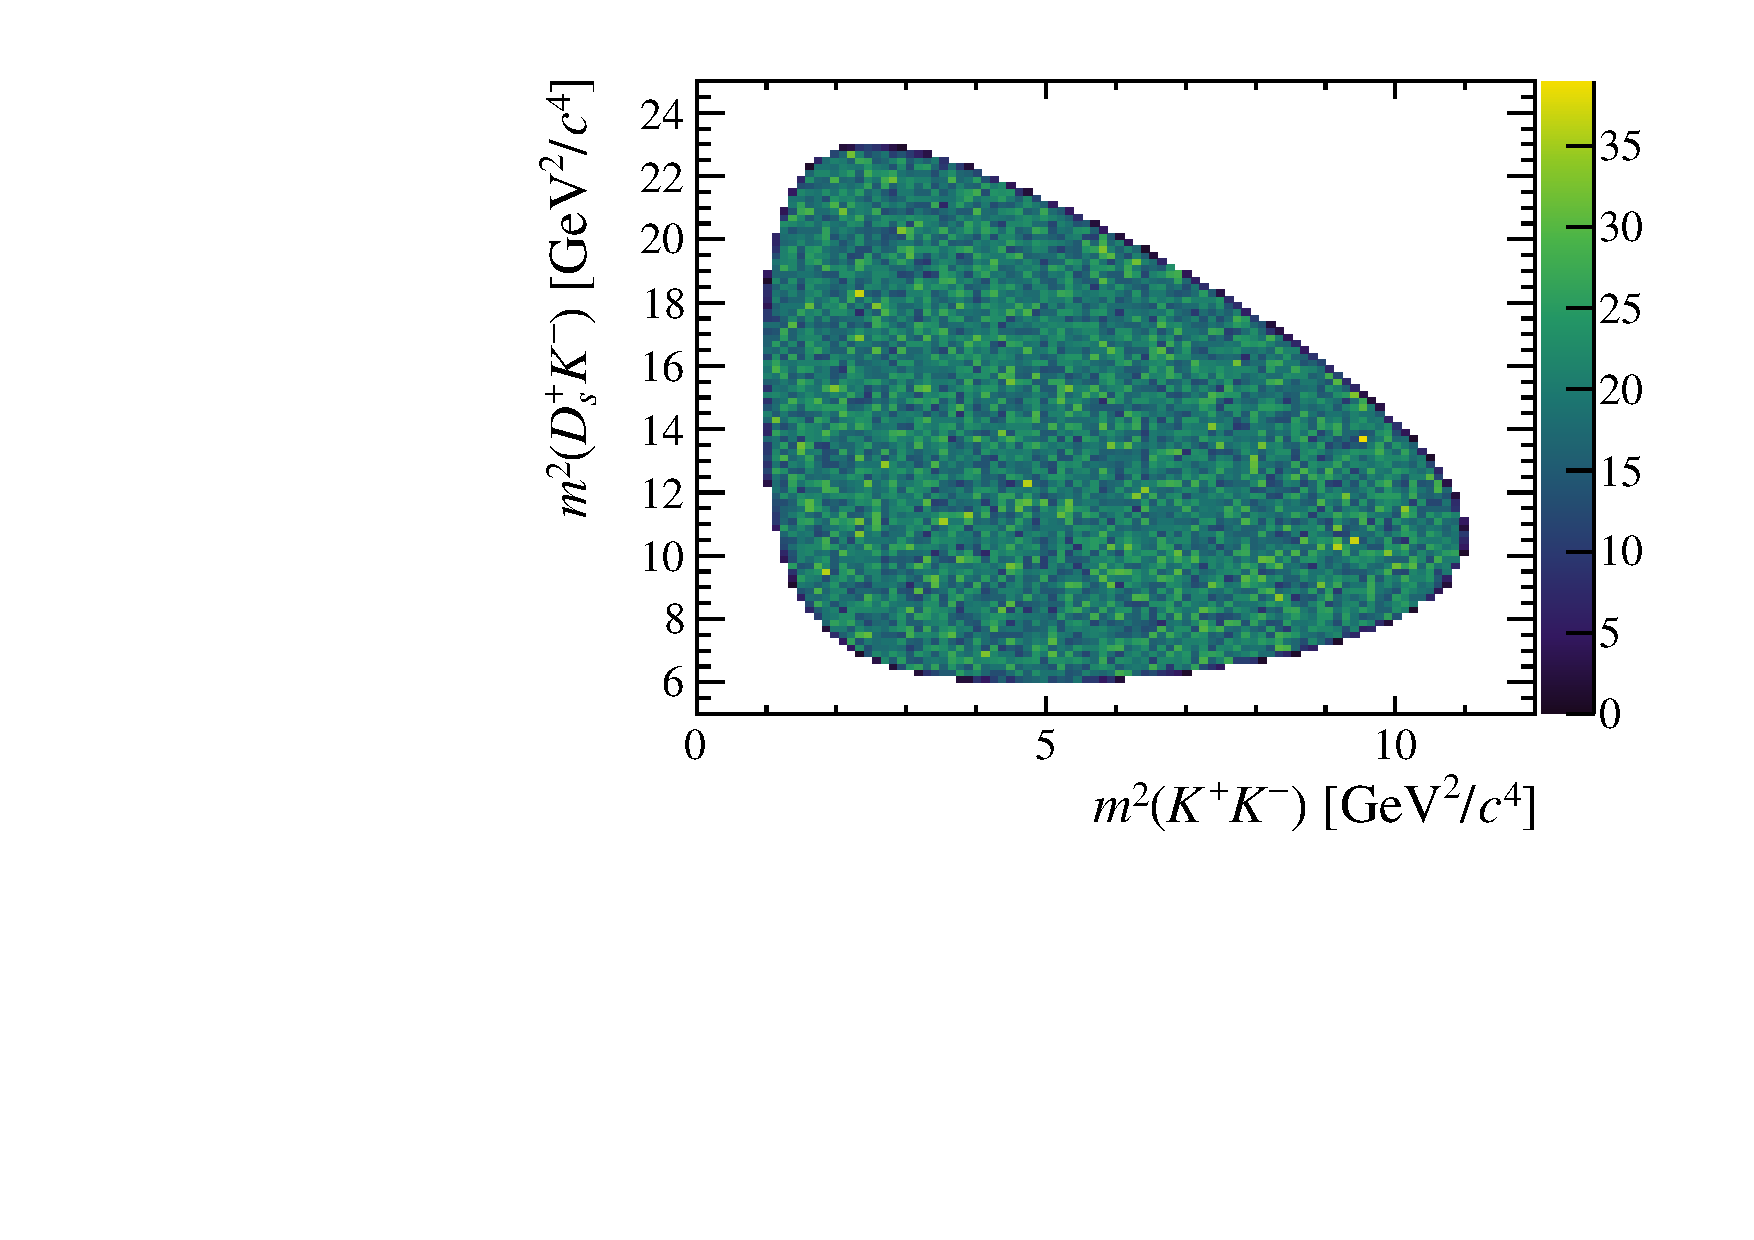
\includegraphics[width=0.32\textwidth]{figs/B2DsPhi/NR_Dalitz_plot.pdf}
%    \caption{The distribution of $m(\Kp\Km)$ (left), Dalitz plot (middle) and the helicity angle $\cos\theta_{K}$ for generated for non-resonant decays.} 
%    \label{fig:DsKK_model_NR}   
% \end{figure}
% %%%%%%%%%%%%%

% \subsubsection{The $f_{0}^{0}(980)$ resonance}

% The $f_{0}^{0}(980)$ resonance is a light unflavoured $J^{P} = 0^{+}$ state with mass $990\pm20\mevcc$ and width 10--100\mevcc~\cite{PDG2016}. It has been observed to decay to $\Kp\Km$ making it a suitable resonance to consider. Although it's mass is at the lower end of the range considered here, it's significant width allows it to contribute at higher invariant masses. This component is modelled with the Flatt\'{e} line shape~\cite{Flatte:1976xu} and the relevant distributions shown in Fig.~\ref{fig:DsKK_model_f0980}.
% %%%%%%%%%%%%%
% \begin{figure}[!h]
%    \centering   
%    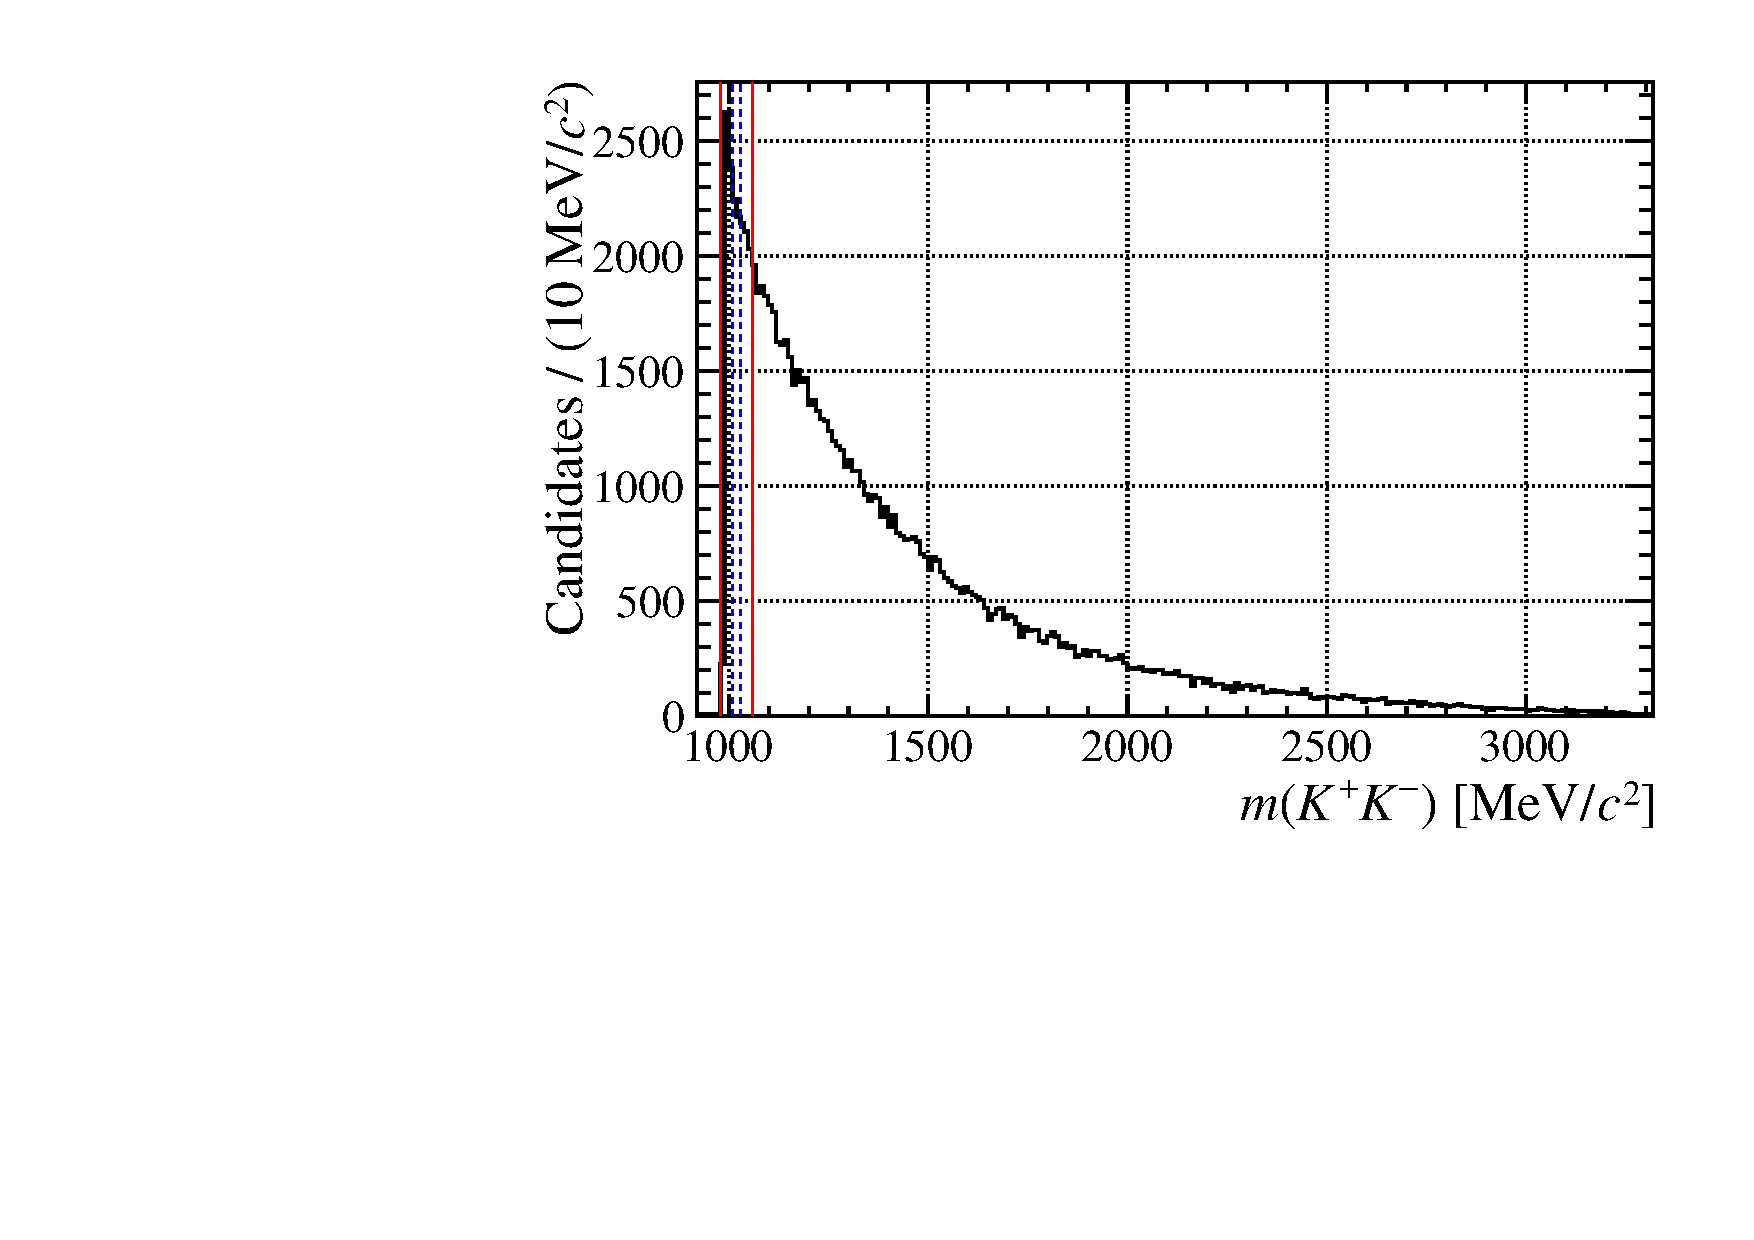
\includegraphics[width=0.32\textwidth]{figs/B2DsPhi/f0_phi_mass.pdf}
%    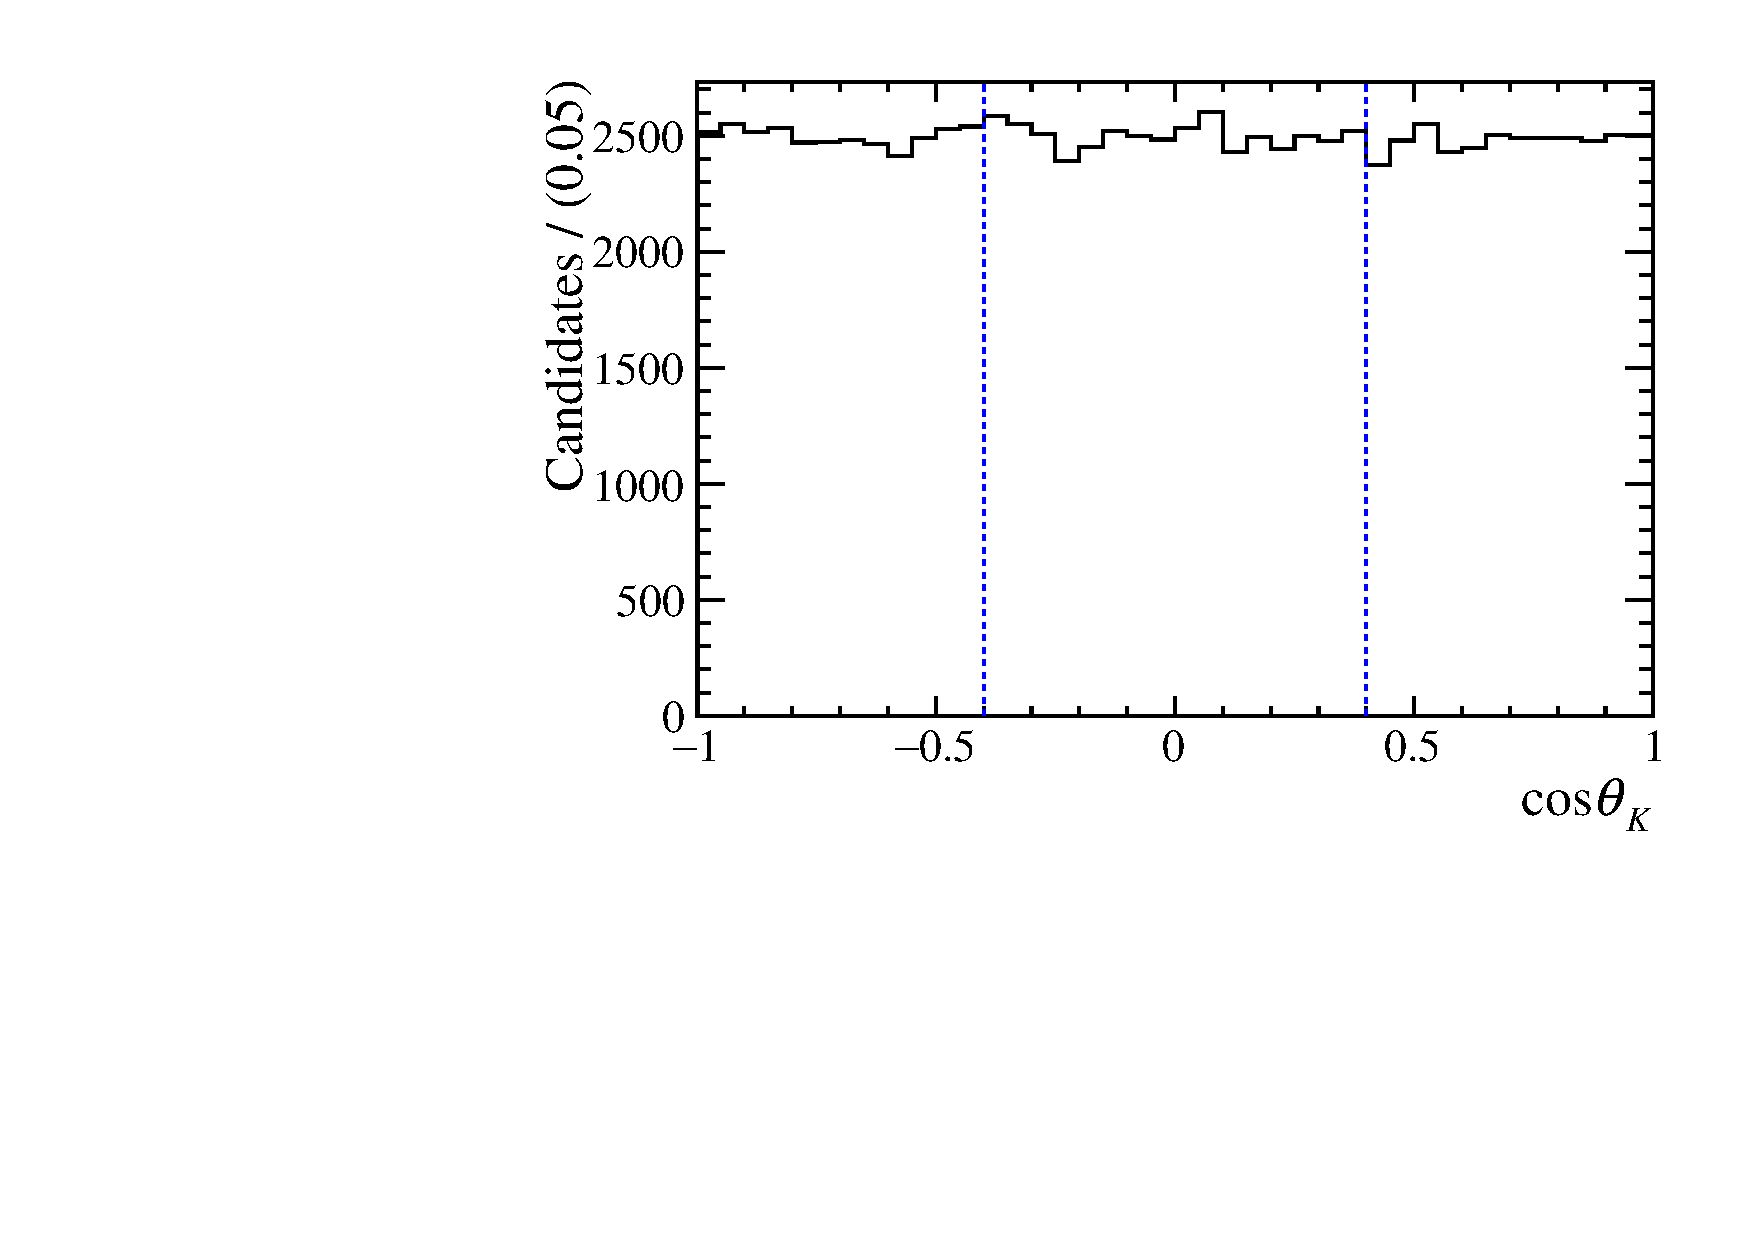
\includegraphics[width=0.32\textwidth]{figs/B2DsPhi/f0_Helicity.pdf}
%    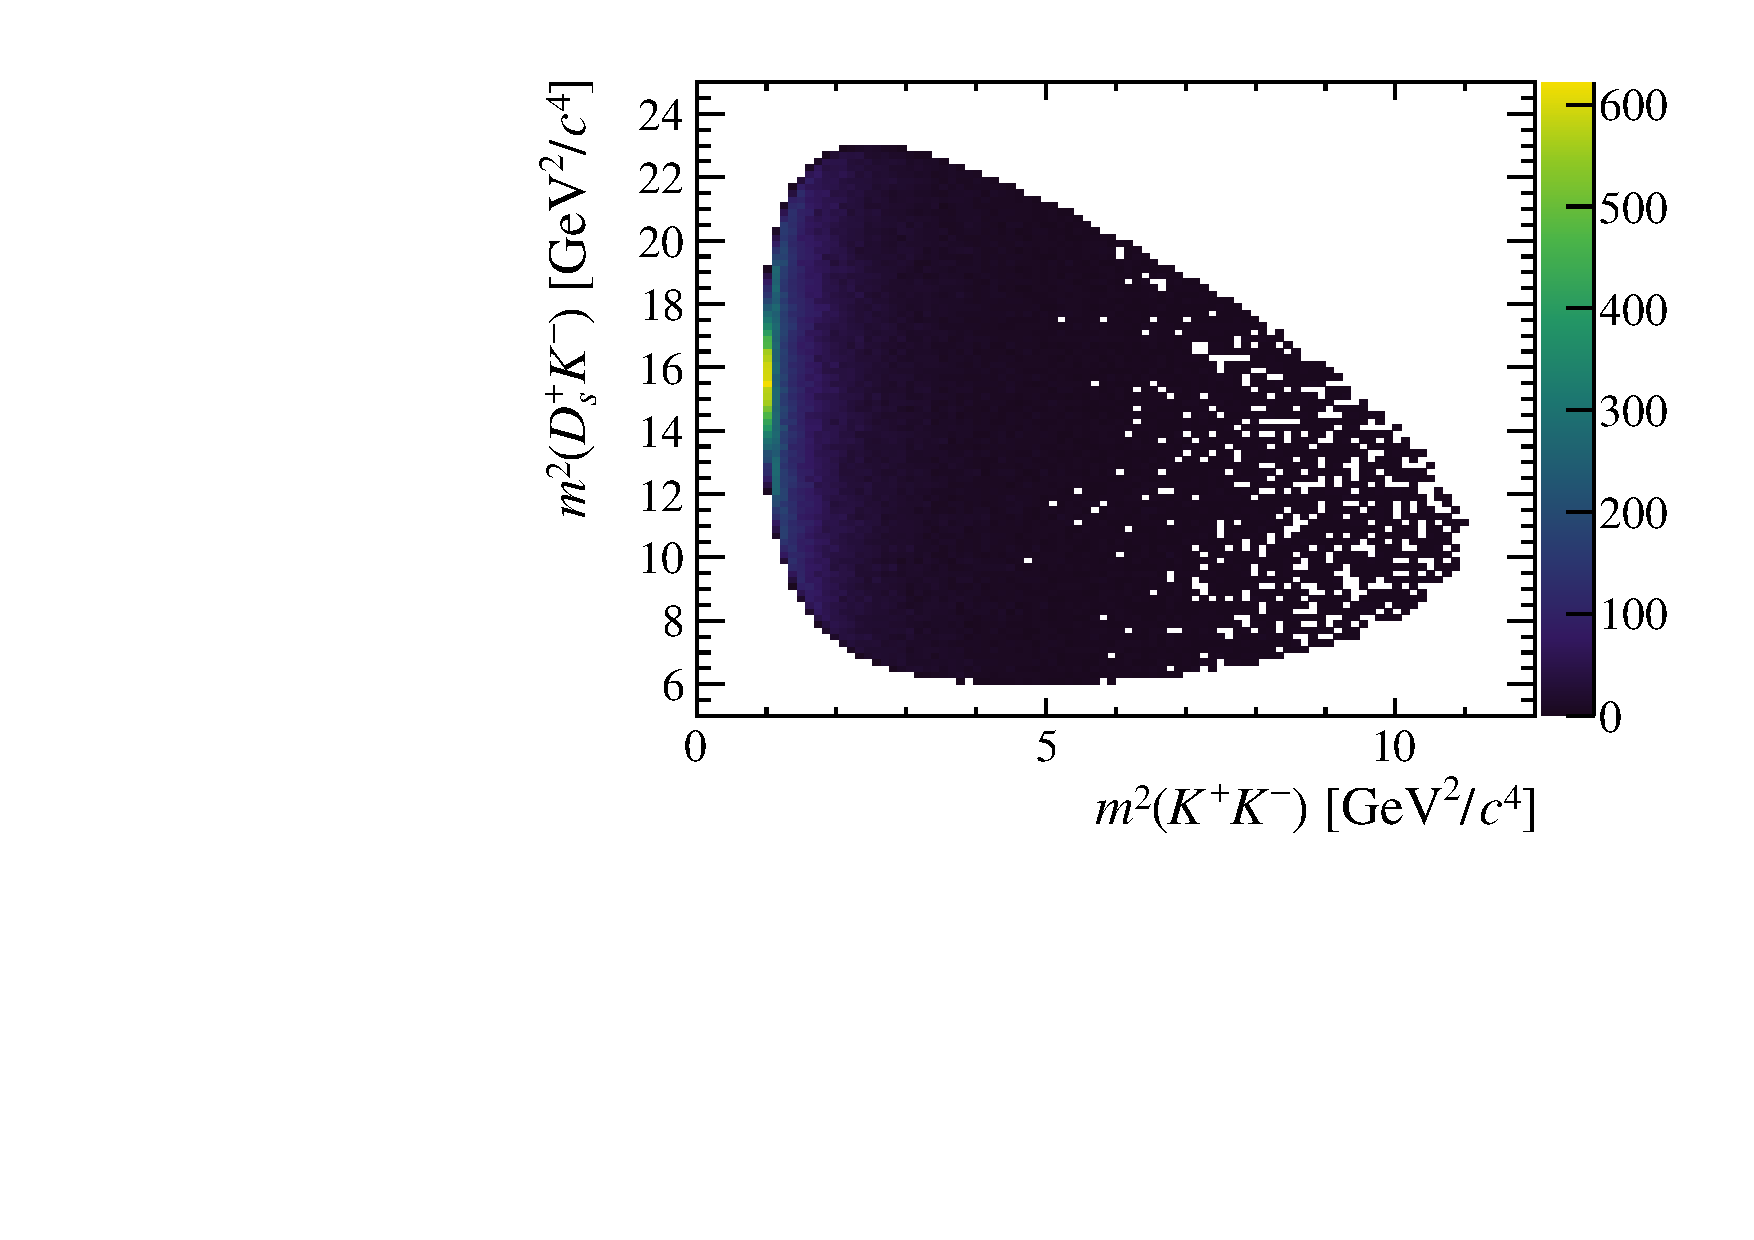
\includegraphics[width=0.32\textwidth]{figs/B2DsPhi/f0_Dalitz_plot.pdf}
%    \caption{The distribution of $m(\Kp\Km)$ (left), Dalitz plot (middle) and the helicity angle $\cos\theta_{K}$ for generated for the $f_{0}^{0}(980)$ resonance.} 
%    \label{fig:DsKK_model_f0980}   
% \end{figure}
% %%%%%%%%%%%%%

% \subsubsection{The $a_{0}^{0}(980)$ resonance}
% The $a_{0}^{0}(980)$ resonance is a light unflavoured $J^{P} = 0^{+}$ state with mass $980\pm20\mevcc$ and width 50--100\mevcc and has been observed to decay to $\PK\Kb$ final states~\cite{PDG2016}. This resonance is also modelled with the Flatt\'{e} line shape and the relevant distributions are shown in Fig~\ref{fig:DsKK_model_a0980}.
% %%%%%%%%%%%%%
% \begin{figure}[!h]
%    \centering   
%    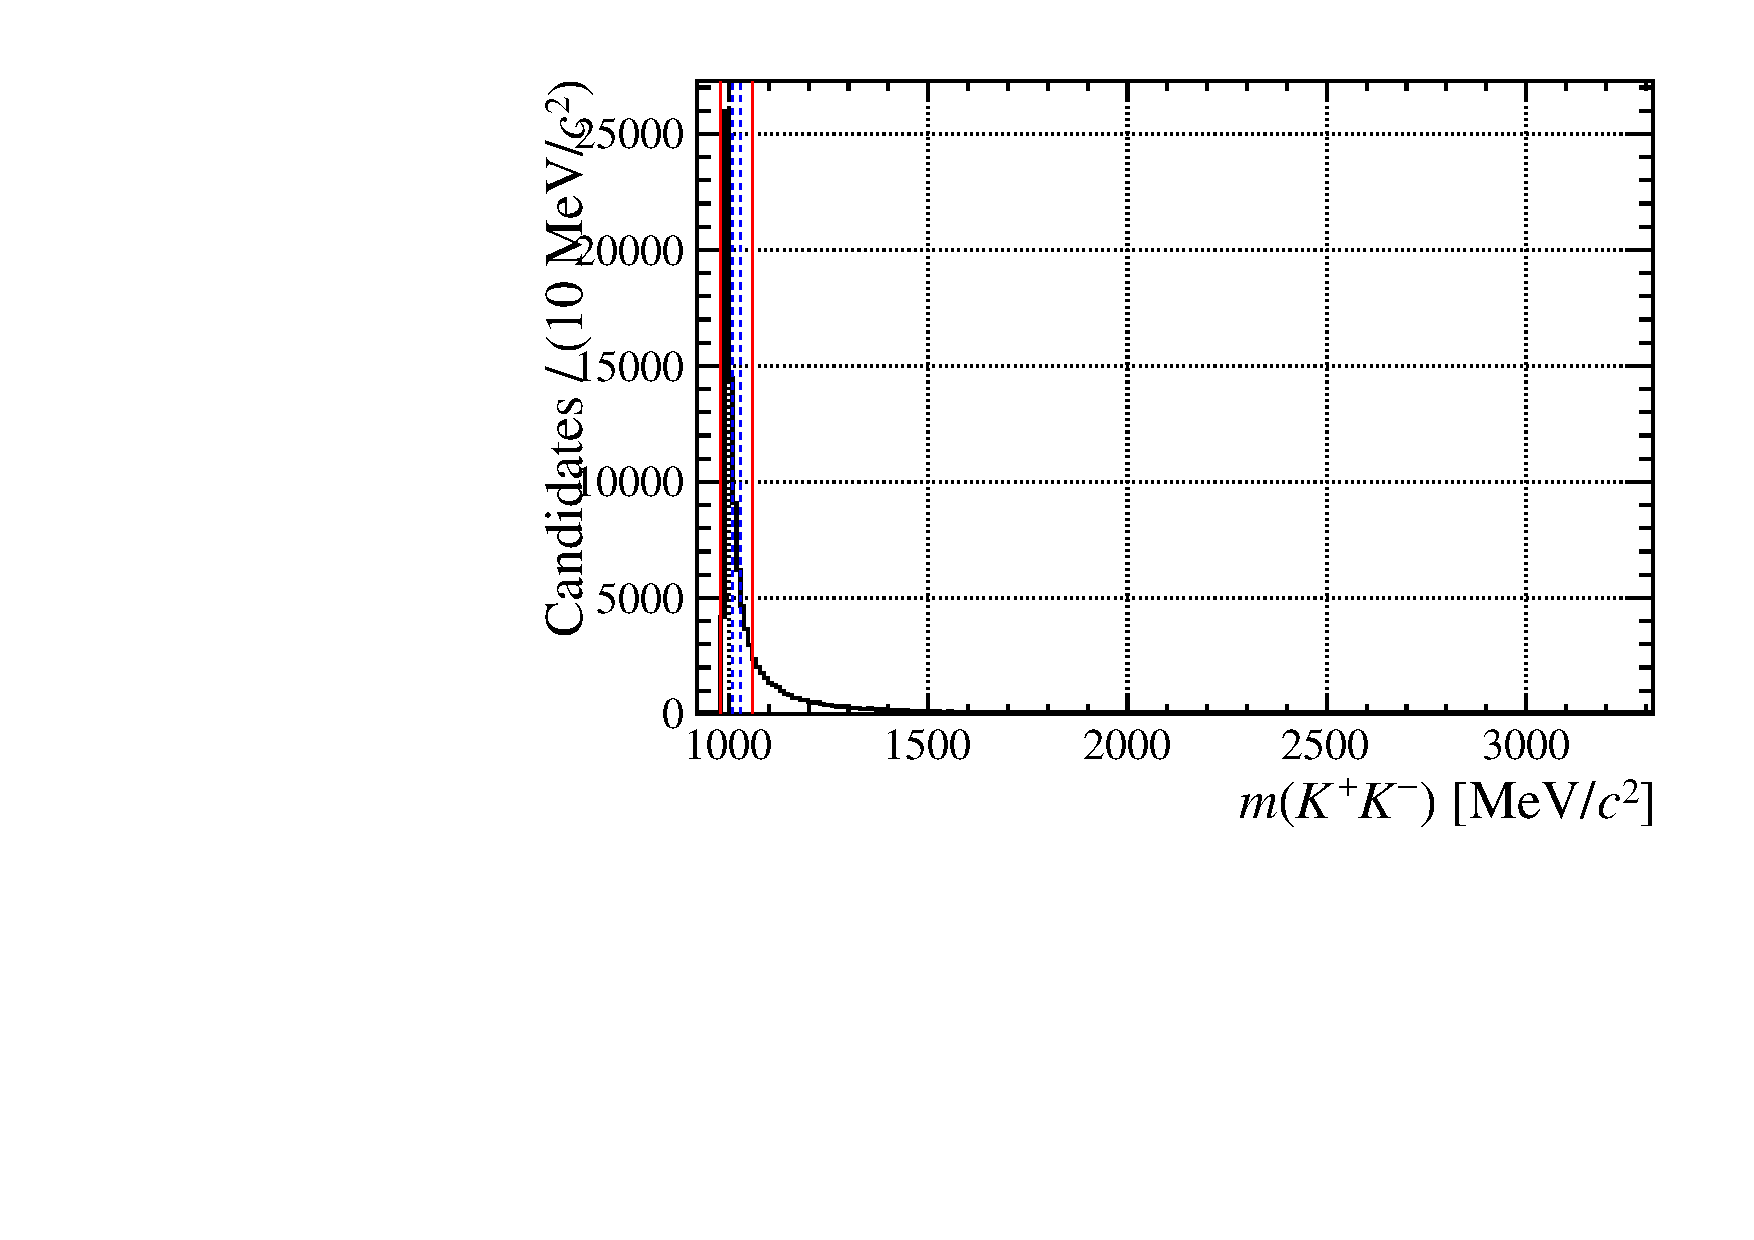
\includegraphics[width=0.32\textwidth]{figs/B2DsPhi/a0_phi_mass.pdf}
%    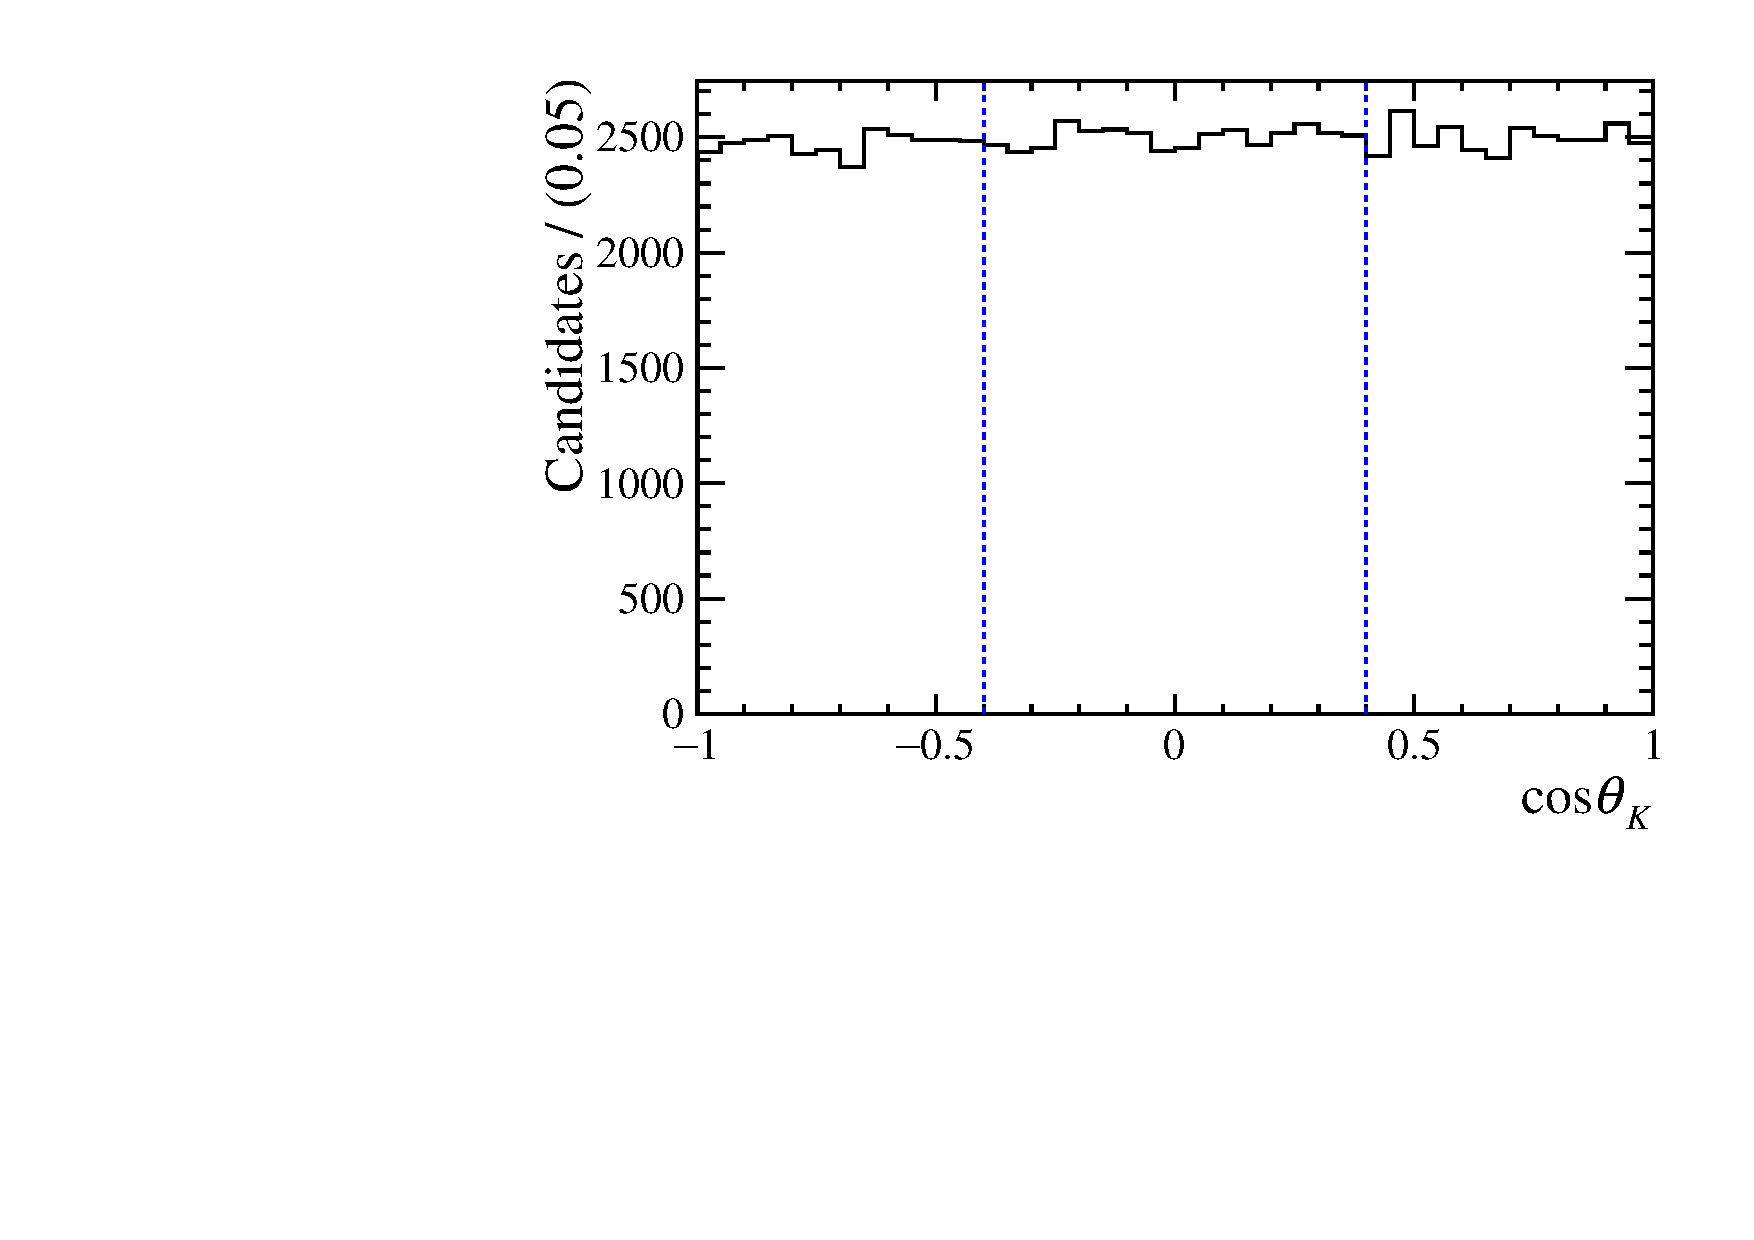
\includegraphics[width=0.32\textwidth]{figs/B2DsPhi/a0_Helicity.pdf}
%    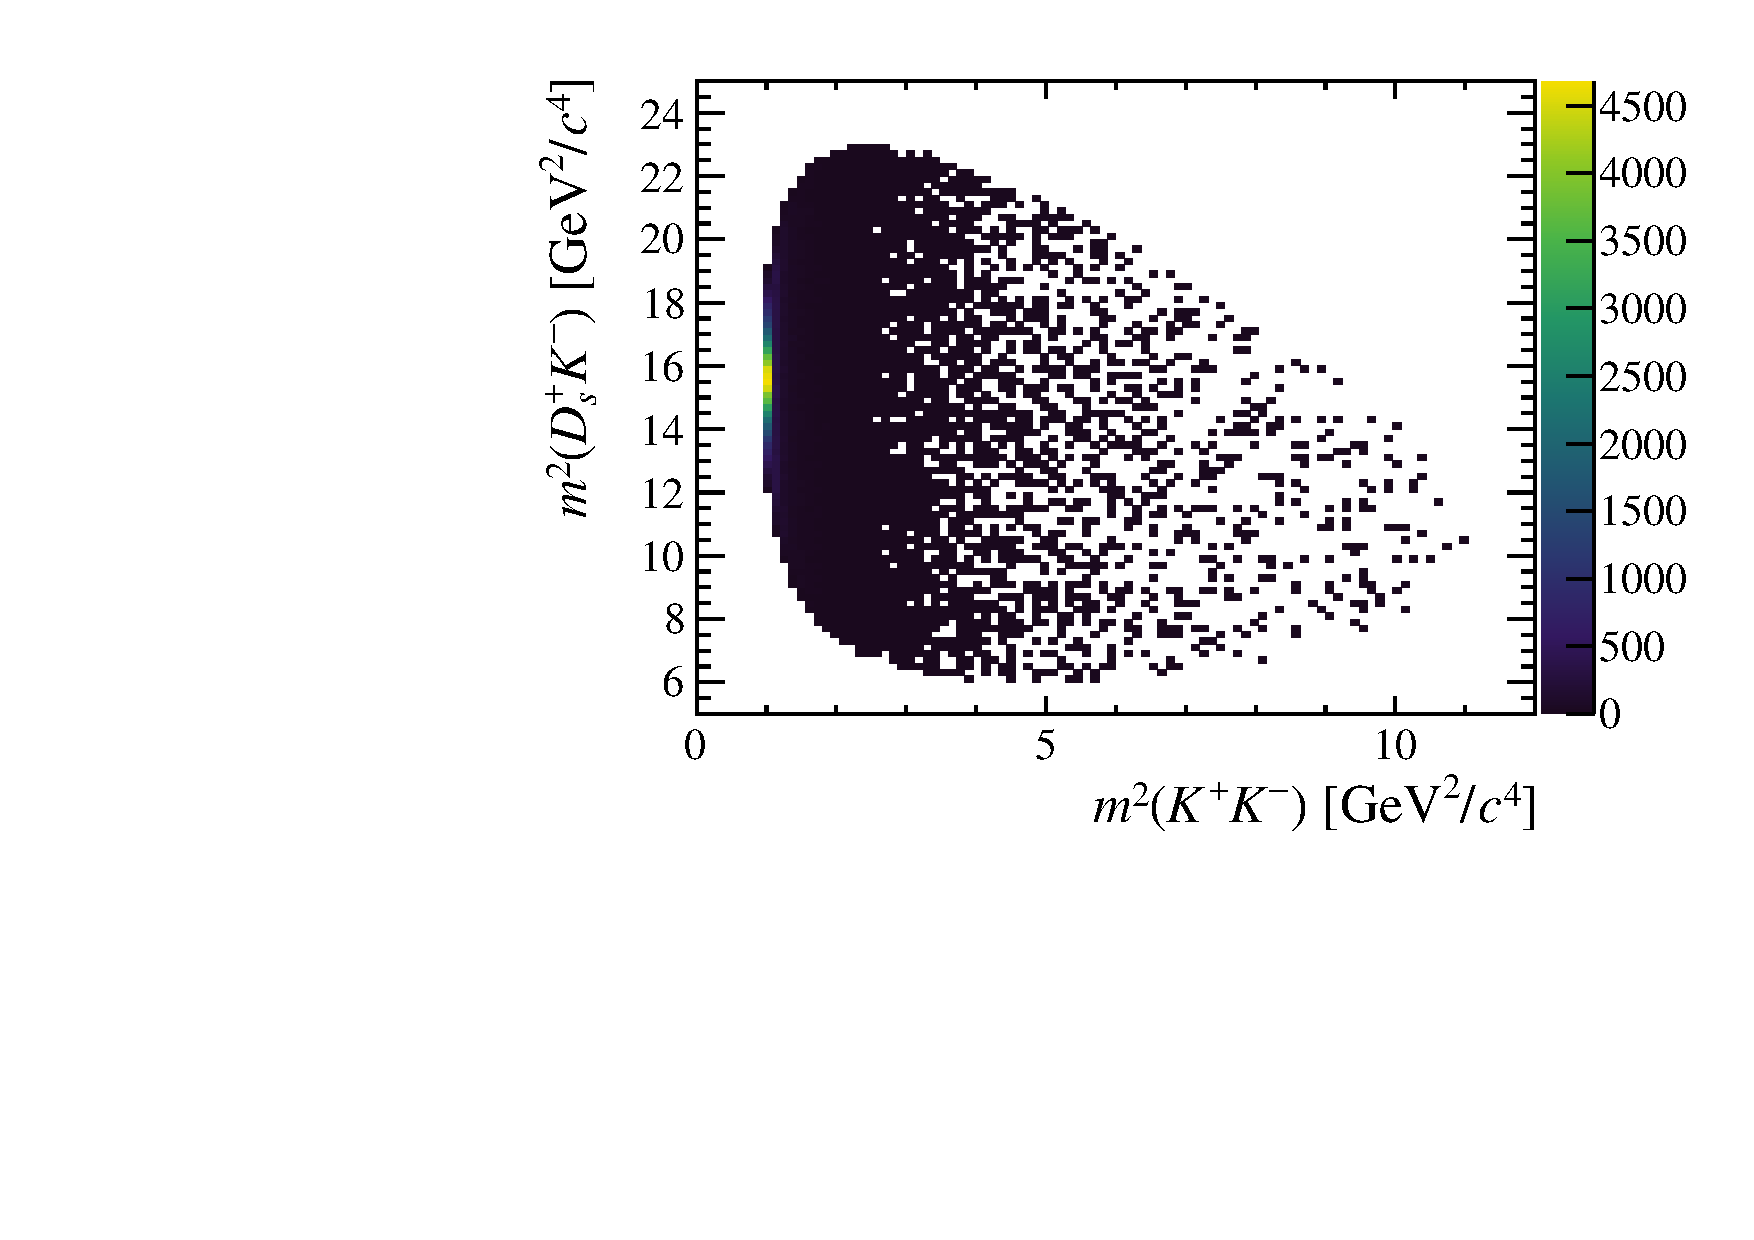
\includegraphics[width=0.32\textwidth]{figs/B2DsPhi/a0_Dalitz_plot.pdf}
%    \caption{The distribution of $m(\Kp\Km)$ (left), Dalitz plot (middle) and the helicity angle $\cos\theta_{K}$ for generated for the $a_{0}^{0}(980)$ resonance.} 
%    \label{fig:DsKK_model_a0980}   
% \end{figure}
% %%%%%%%%%%%%%

% \subsubsection{The $f_{0}^{0}(1370)$ resonance}
% The $f_{0}^{0}(1370)$ resonance is a light unflavoured $J^{P} = 0^{+}$ state with a mass in the range 1200--1500\mevcc and width in the range 200--500\mevcc. It has been observed to decay to the \kaon\Kb final states. It is modelled with a Relativistic Breit-Wigner line shape and the relevant distributions are shown in Fig.~\ref{fig:DsKK_model_f01370}.
% %%%%%%%%%%%%%
% \begin{figure}[!h]
%    \centering   
%    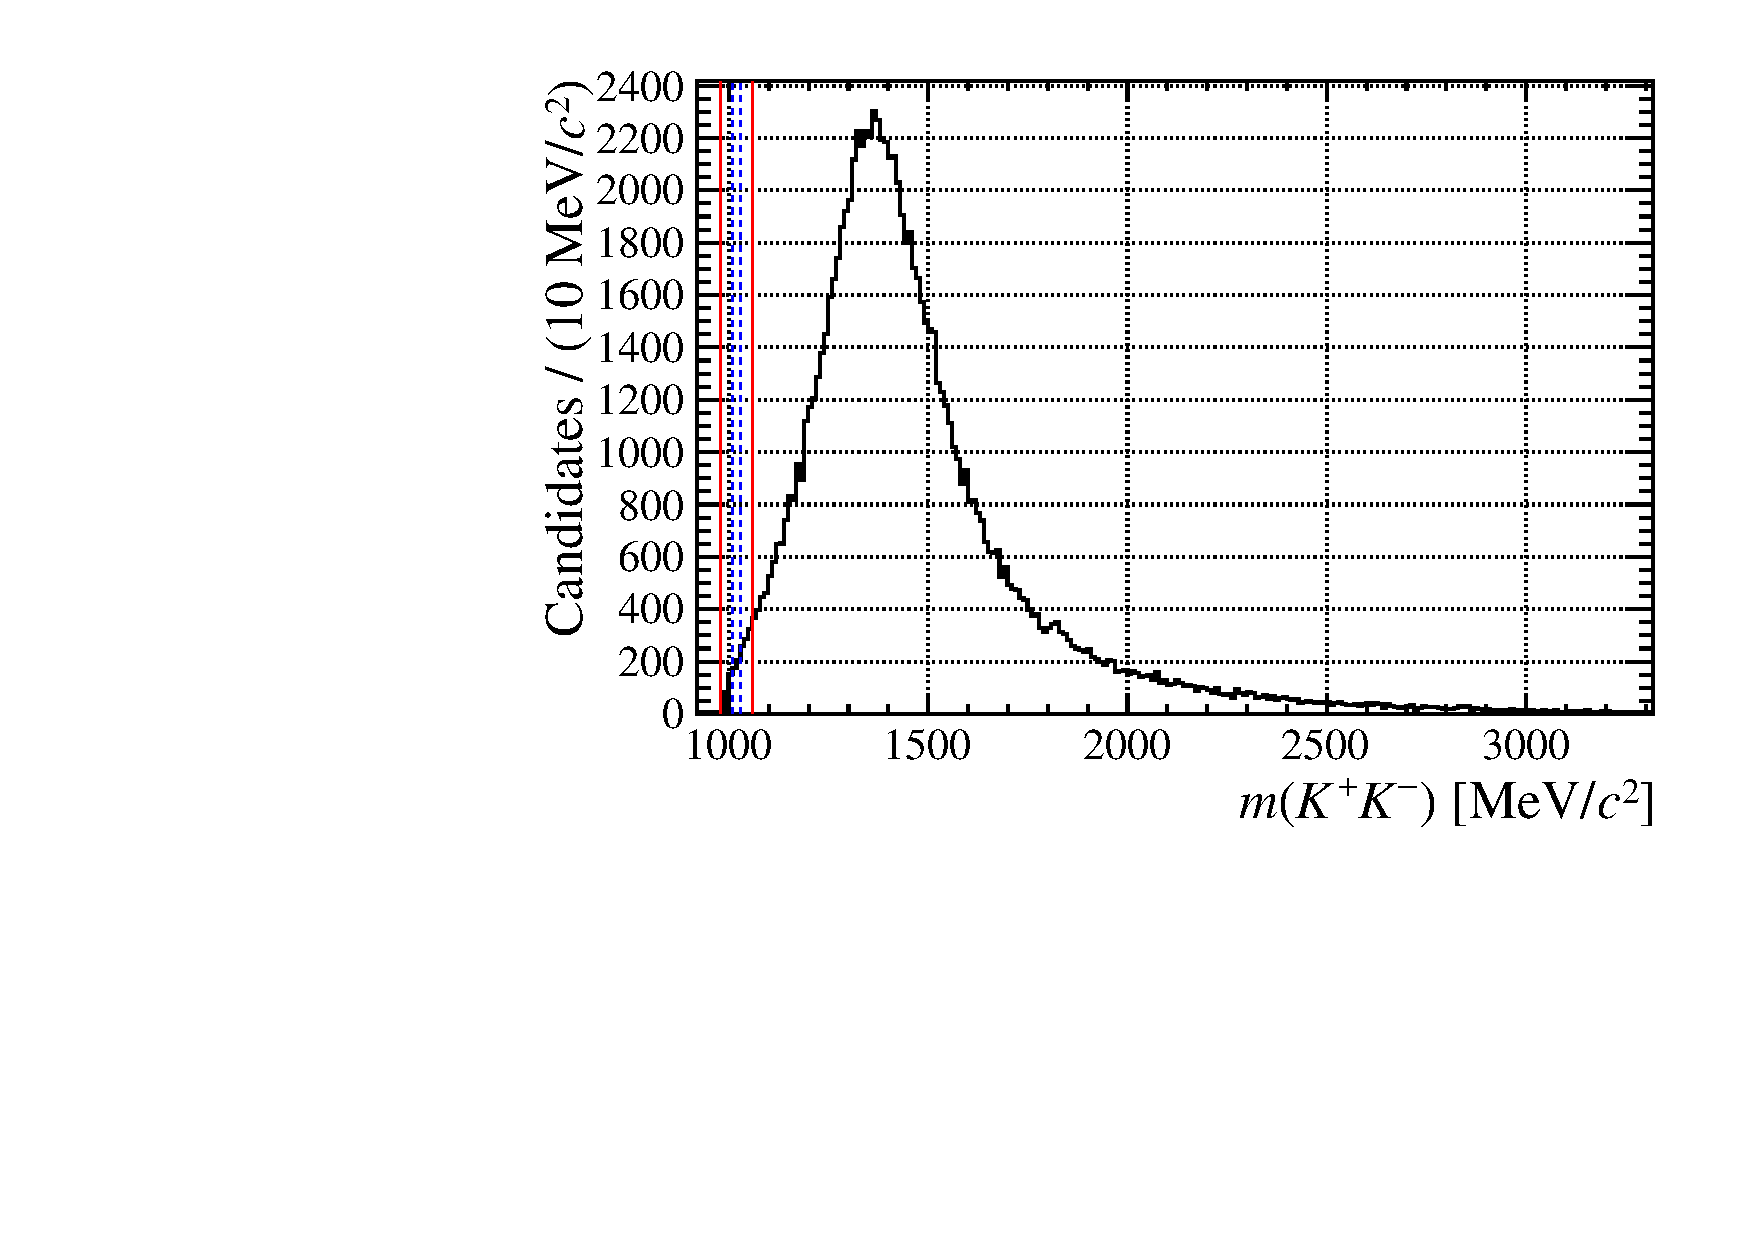
\includegraphics[width=0.32\textwidth]{figs/B2DsPhi/f0_1370_phi_mass.pdf}
%    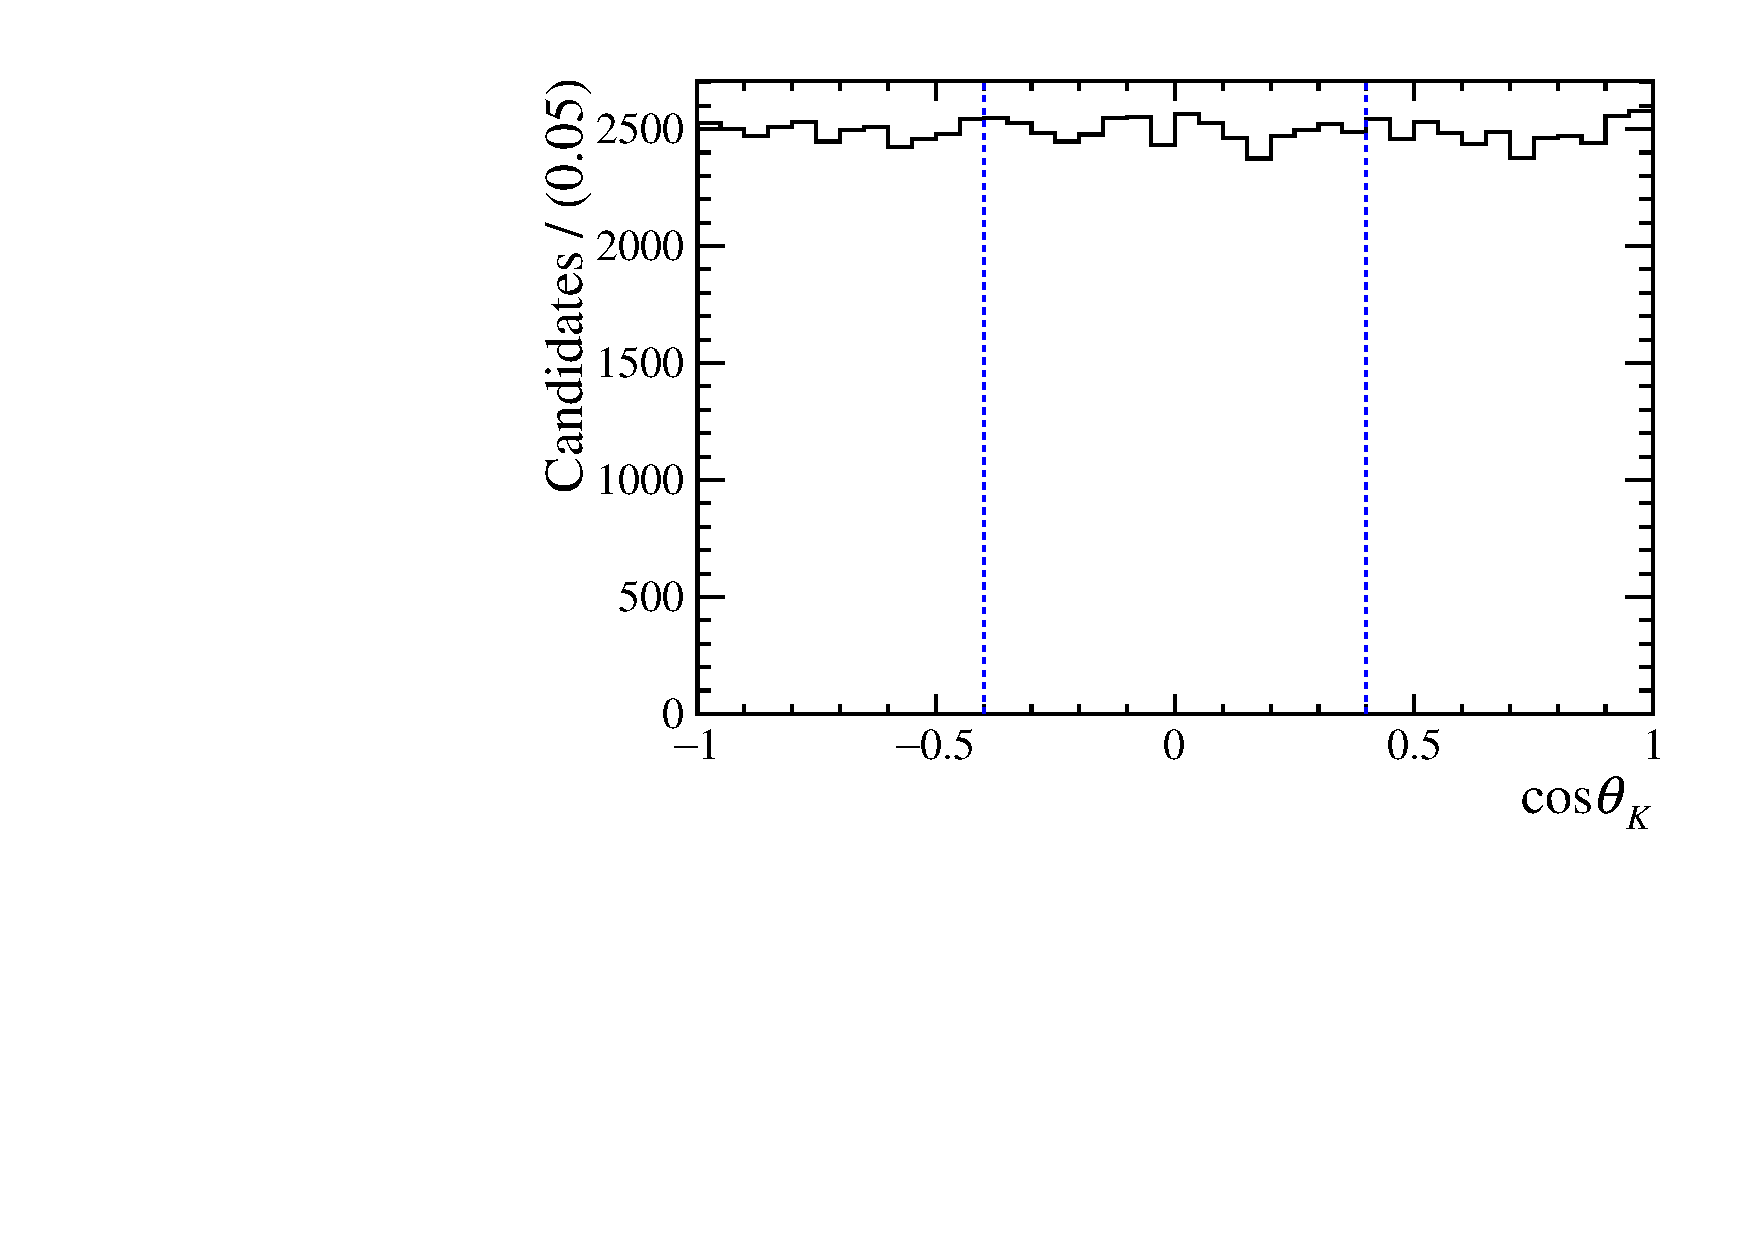
\includegraphics[width=0.32\textwidth]{figs/B2DsPhi/f0_1370_Helicity.pdf}
%    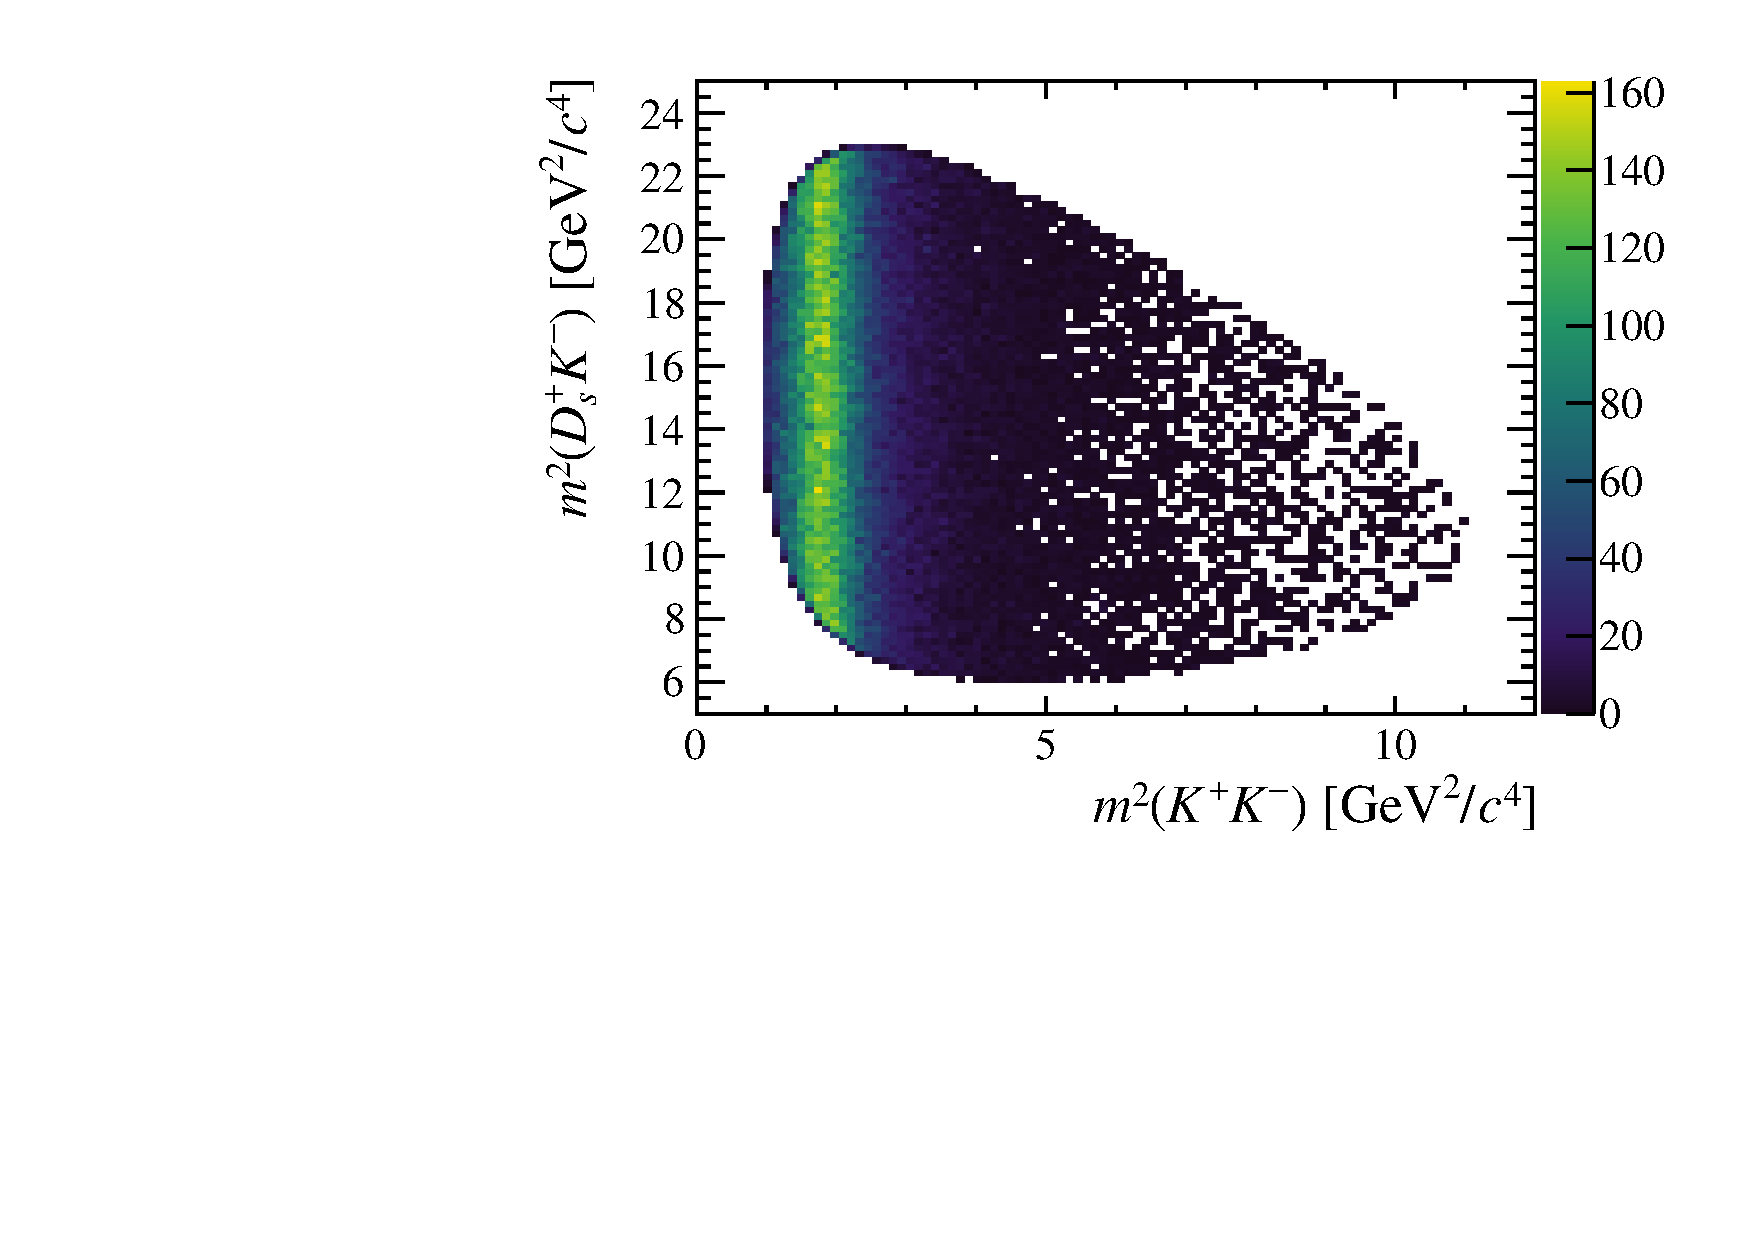
\includegraphics[width=0.32\textwidth]{figs/B2DsPhi/f0_1370_Dalitz_plot.pdf}
%    \caption{The distribution of $m(\Kp\Km)$ (left), Dalitz plot (middle) and the helicity angle $\cos\theta_{K}$ for generated for the $f_{0}^{0}(1370)$ resonance.} 
%    \label{fig:DsKK_model_f01370}   
% \end{figure}
% %%%%%%%%%%%%%

% \subsubsection{The $f_{2}^{0}(1270)$ resonance}
% The $f_{2}^{0}(1270)$ resonance is a $J^{P} = 2^{+}$ state with mass $1275.5\pm08\mevcc$ and width $186.7^{+2.2}_{-2.5}\mevcc$ that has been observed to decay to \kaon\Kb final states. This resonance is modelled with a Relativistic Breit-Wigner line shape as shown in Fig.~\ref{fig:DsKK_model_f21270}.

% %%%%%%%%%%%%%
% \begin{figure}[!h]
%    \centering   
%    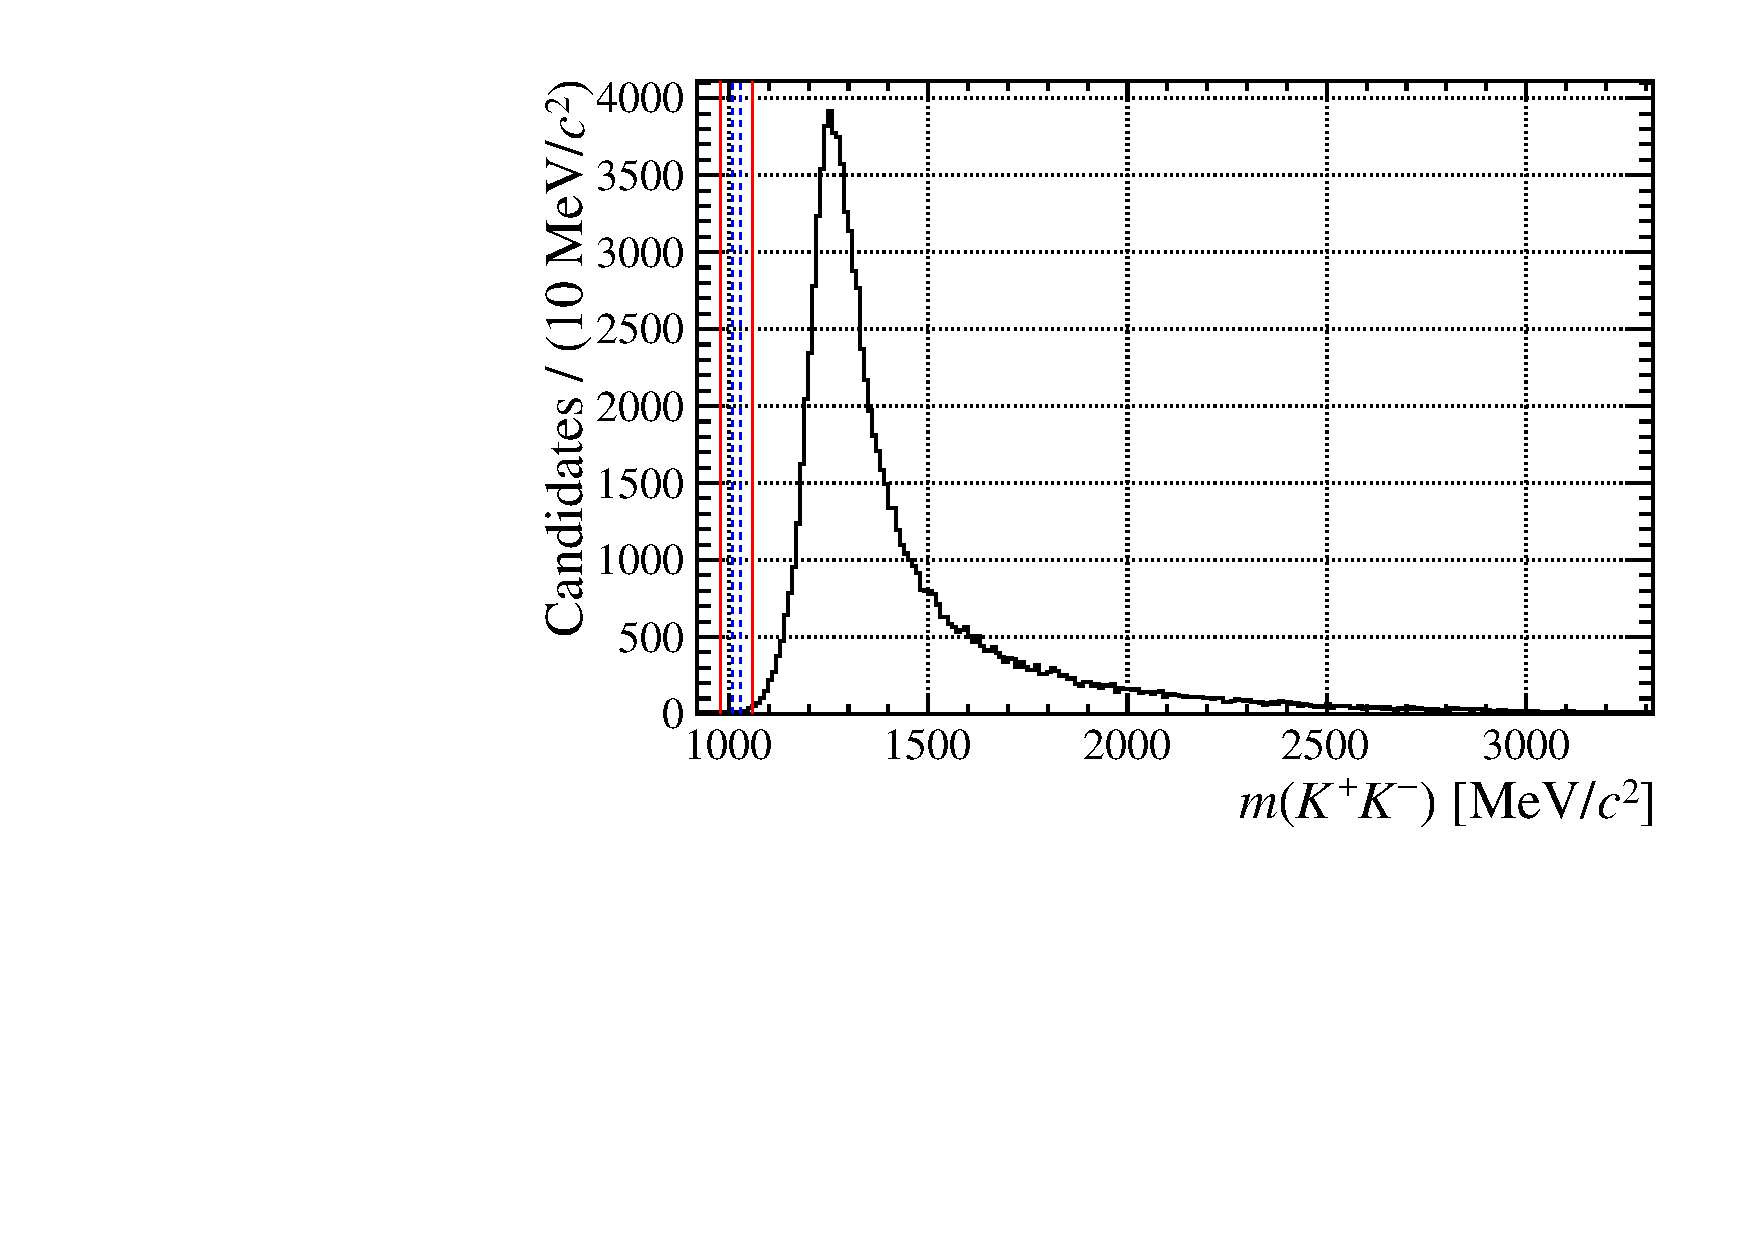
\includegraphics[width=0.32\textwidth]{figs/B2DsPhi/f2_phi_mass.pdf}
%    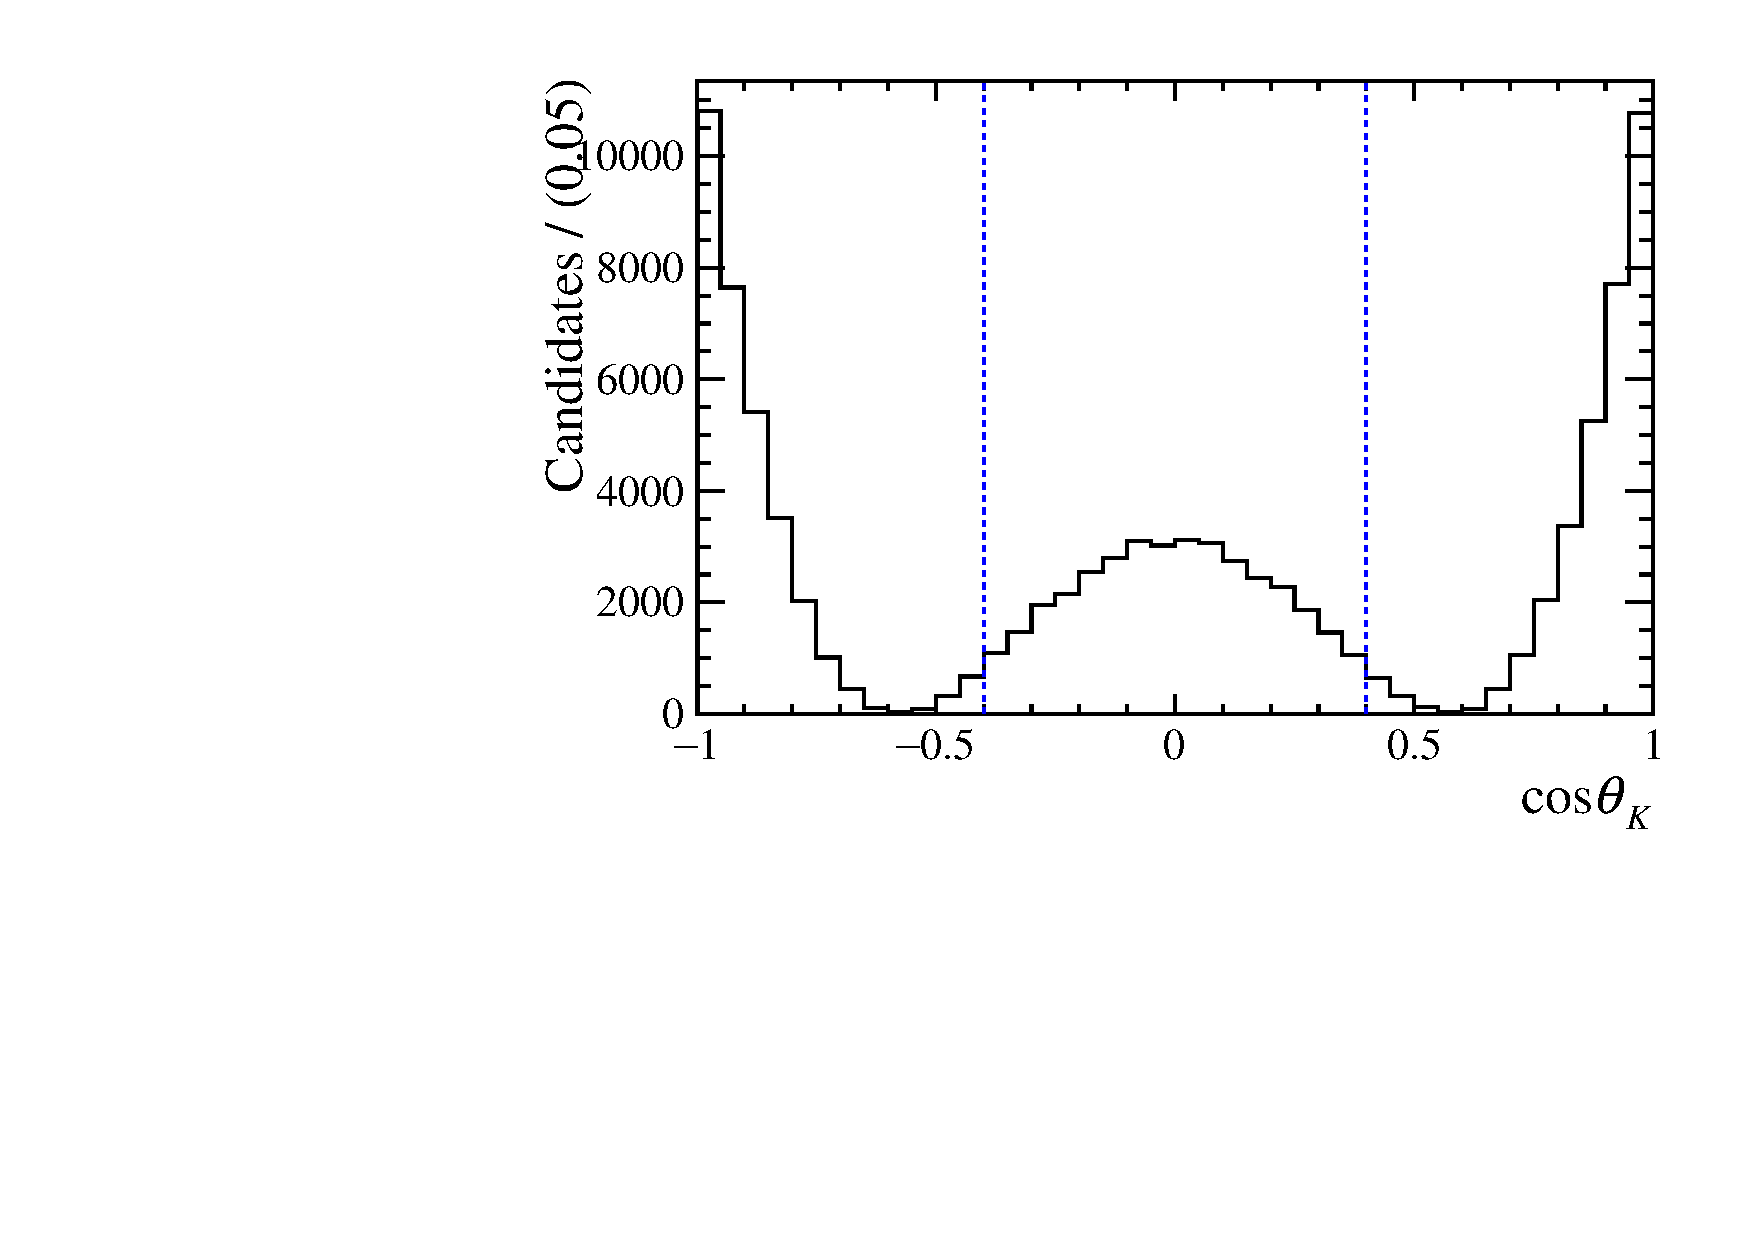
\includegraphics[width=0.32\textwidth]{figs/B2DsPhi/f2_Helicity.pdf}
%    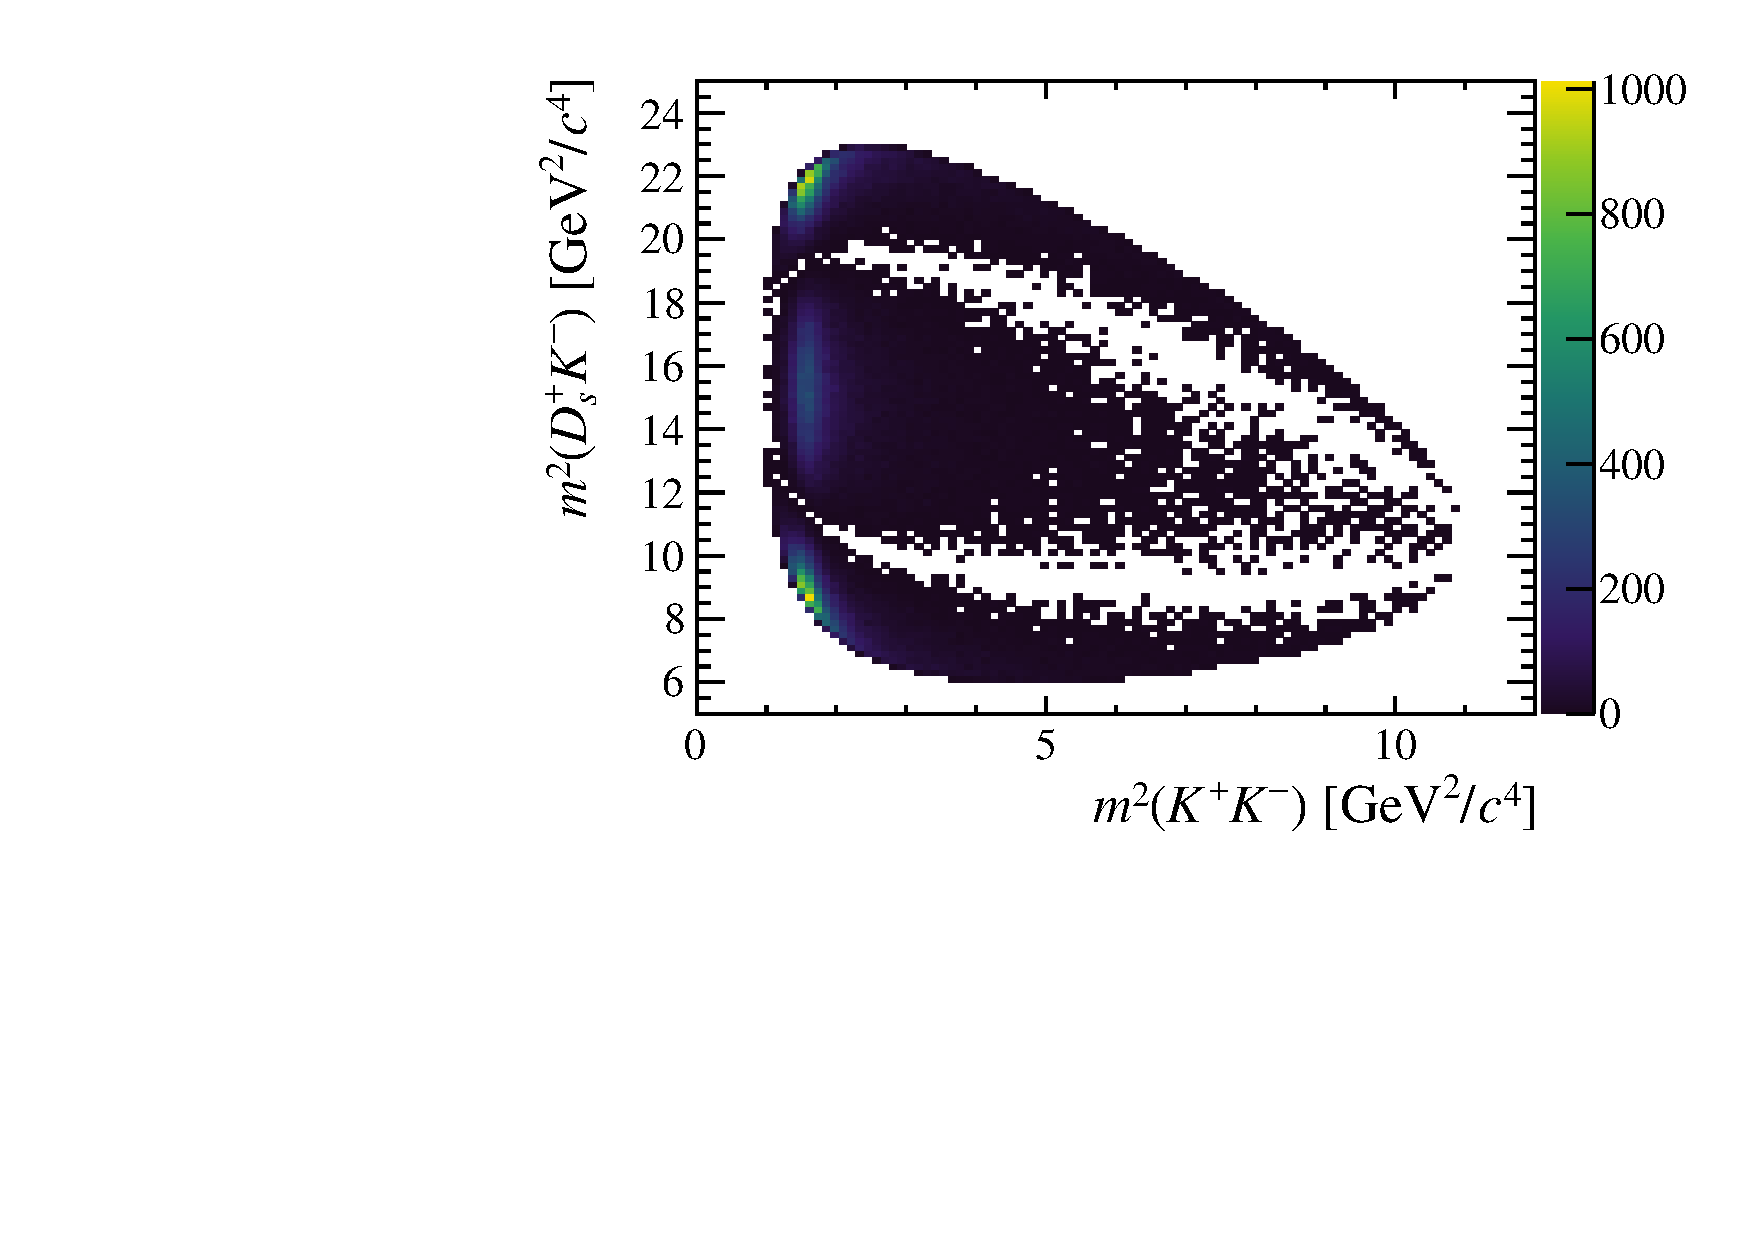
\includegraphics[width=0.32\textwidth]{figs/B2DsPhi/f2_Dalitz_plot.pdf}
%    \caption{The distribution of $m(\Kp\Km)$ (left), Dalitz plot (middle) and the helicity angle $\cos\theta_{K}$ for generated for the $f_{2}^{0}(1270)$ resonance.} 
%    \label{fig:DsKK_model_f21270}   
% \end{figure}
% %%%%%%%%%%%%%


% \subsubsection{The $a_{2}^{0}(1320)$ resonance}
% The $a_{2}^{0}(1320)$ resonance is a $J^{P} = 2^{+}$ state with a mass $1318.1\pm0.7\mevcc$ and width $109.8\pm2.4\mevcc$ (both measured in the \kaon\Kb mode) observed decaying to the \kaon\Kb final state. This resonance is modelled with a Relativistic Breit-Wigner line shape and shown in Fig.~\ref{fig:DsKK_model_a21320}.
% %%%%%%%%%%%%%
% \begin{figure}[!h]
%    \centering   
%    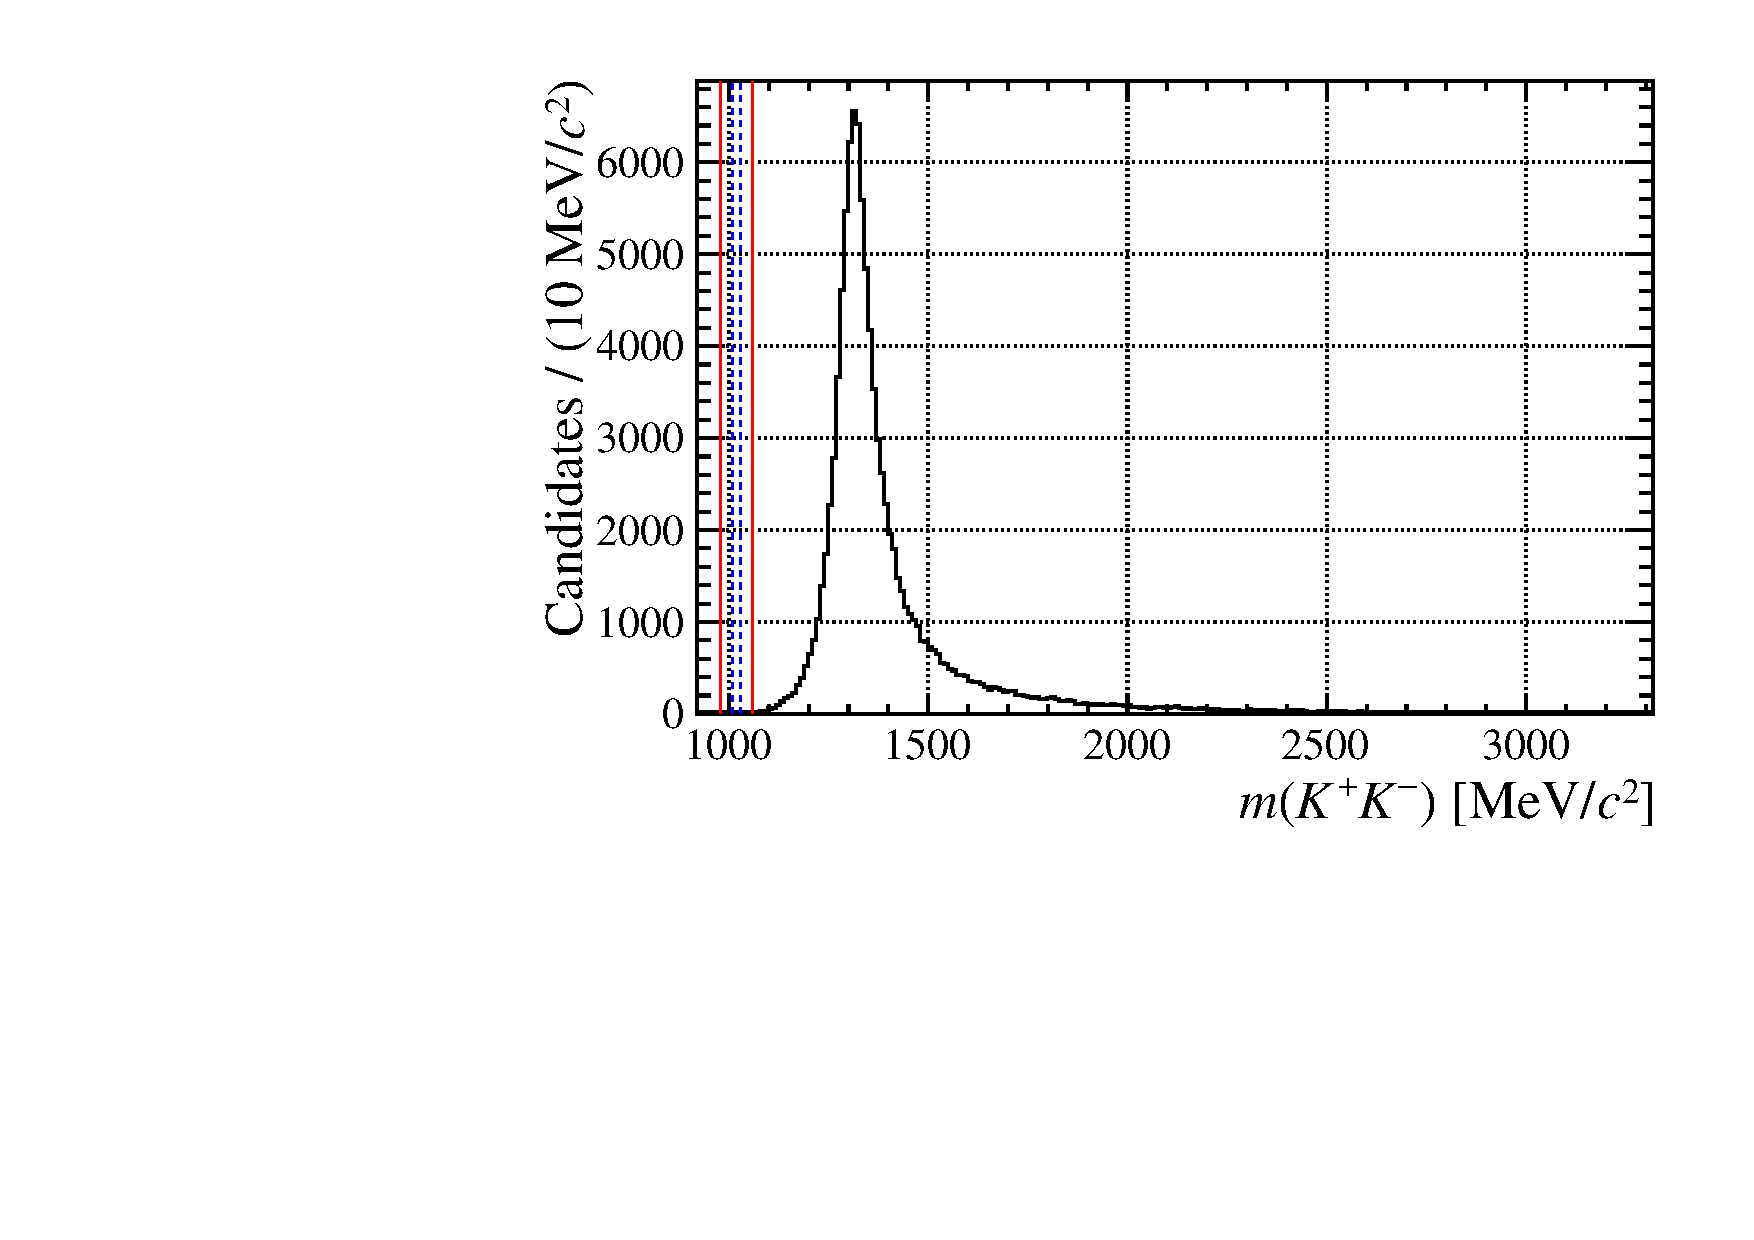
\includegraphics[width=0.32\textwidth]{figs/B2DsPhi/a2_1320_phi_mass.pdf}
%    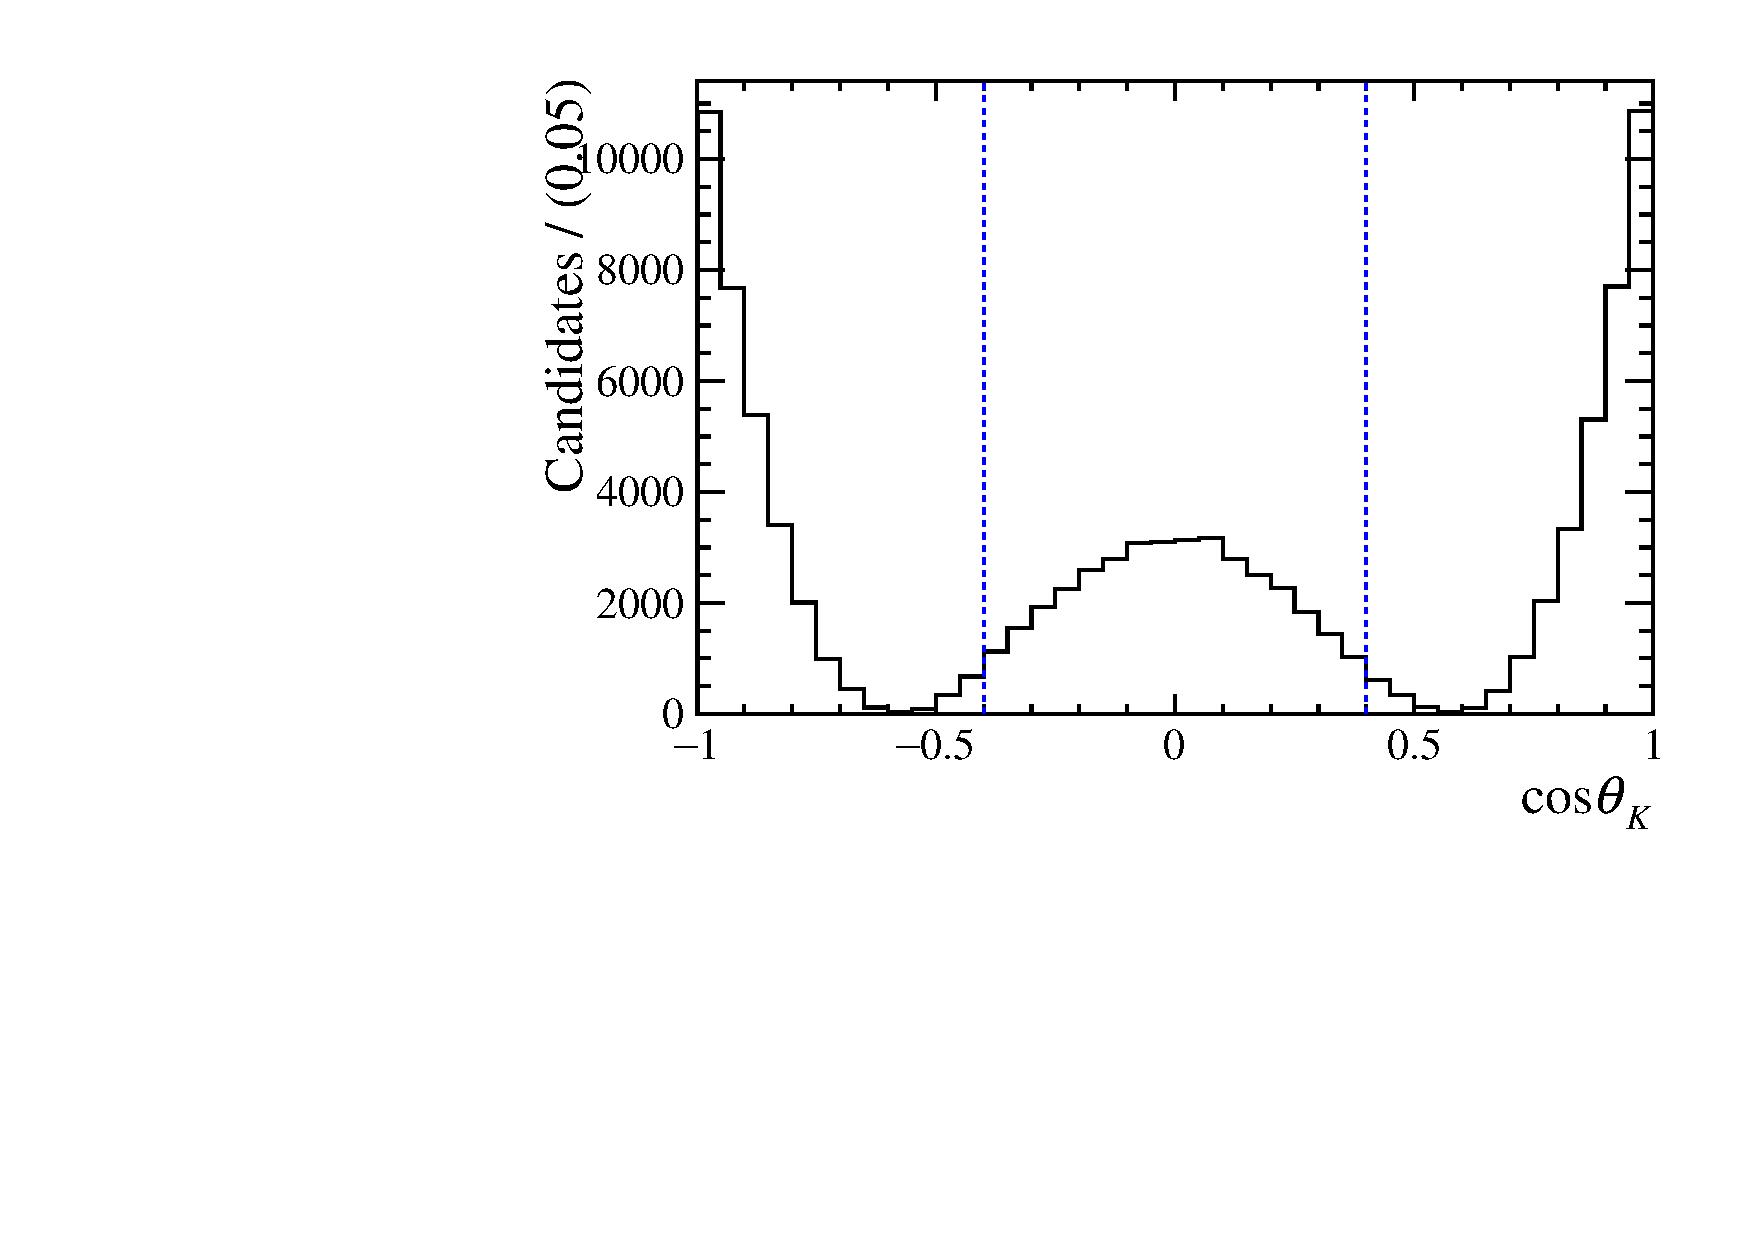
\includegraphics[width=0.32\textwidth]{figs/B2DsPhi/a2_1320_Helicity.pdf}
%    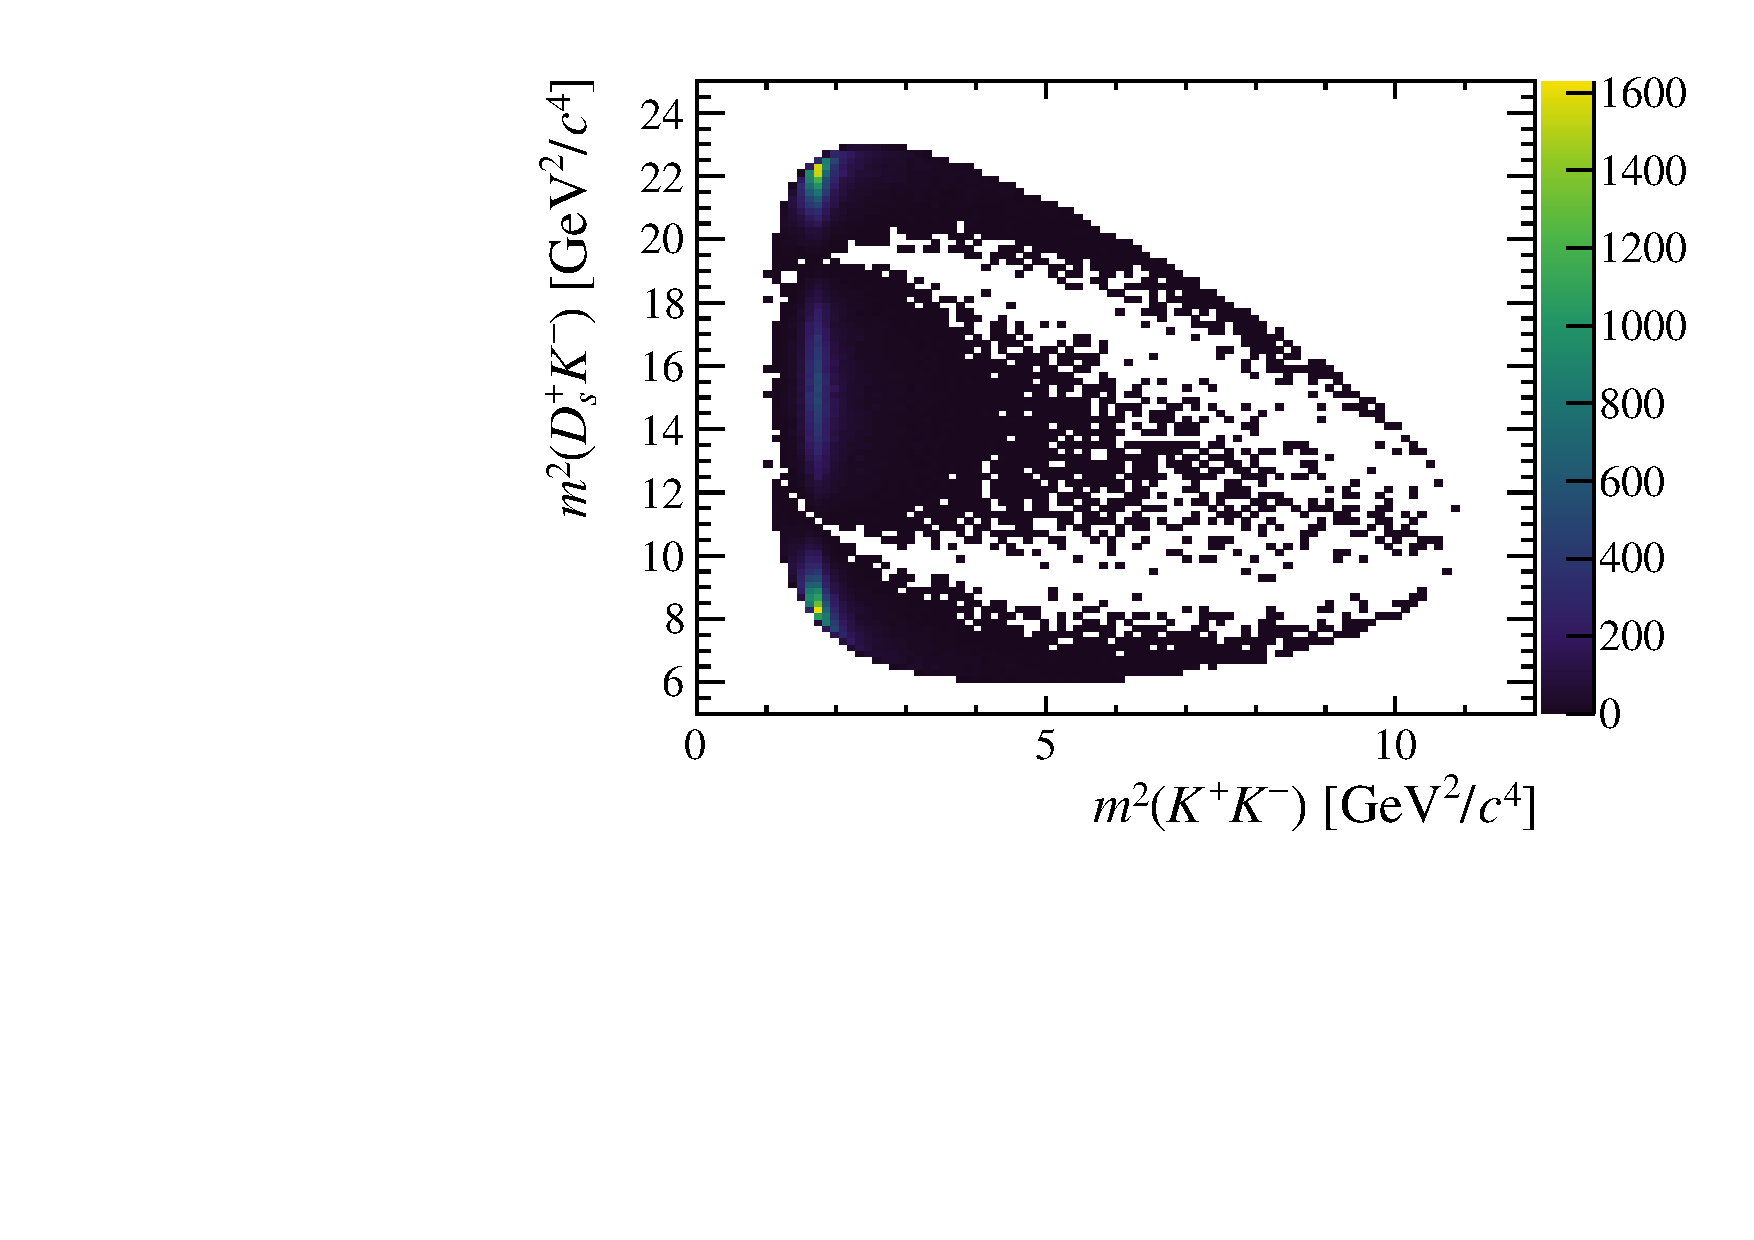
\includegraphics[width=0.32\textwidth]{figs/B2DsPhi/a2_1320_Dalitz_plot.pdf}
%    \caption{The distribution of $m(\Kp\Km)$ (left), Dalitz plot (middle) and the helicity angle $\cos\theta_{K}$ for generated for the $a_{2}^{0}(1320)$ resonance.} 
%    \label{fig:DsKK_model_a21320}   
% \end{figure}
% %%%%%%%%%%%%%


%%%%%%%%%%%%%%====================
%%%%%%%%%%%%%%====================

In Section~\ref{sec:B2DsKK_possible_res}, the possible contributions to \decay{\Bp}{\Dsp\Kp\Km} decays in the region of the \phiz-meson mass are discussed. The points considered leave the $f_{0}^{0}(980)$ and $a_{0}^{0}(980)$ resonances as possible contributions. 
The fraction of decays expected in each $m(\Kp\Km)$ and $\cos\theta_{K}$ category for the different models considered are tabulated in Table~\ref{table:DsKK_rescfracs}. These are calculated by counting the numbers of entries in the corresponding ranges delineated by the vertical lines in Figs.~\ref{fig:DsKK_model_phi1020}-\ref{fig:DsKK_model_a21320}. For reference, the $\phi(1020)$ fractions are included for both the fully simulated decays and those generated with \laurapp. The maximum difference between these fractions is included as a source of systematic uncertainty in Sec.~\ref{sec:B2DsPhi_systuncertainy}.
between It is clear that the \phiz resonance has significantly different fractions in each category for all of the models considered, allowing the component to be distinguished.   



The fractions of \decay{\Bp}{\Dsp\Kp\Km} decays that have been used in the fit model are fixed to the average of the $f_{0}^{0}(980)$ and $a_{0}^{0}(980)$ resonance fractions, listed in the final row of Table~\ref{table:DsKK_rescfracs}. Uncertainties are assigned that correspond to half the difference of the two values. These uncertainties are propagated to the $\BF(\decay{\Bp}{\Dsp\phiz})$ branching fraction in Sec.~\ref{sec:B2DsPhi_systuncertainy}. 


%%%%%%%%%%%%%%%%%%%%%%%%%%%%%%%%%%%%%%%%%%%%%%%%%%%%%%%%%% 
% Table of things
%%%%%%%%%%%%%%%%%%%%%%%%%%%%%%%%%%%%%%%%%%%%%%%%%%%%%%%%%% 
\begin{table}[!ht]
   \centering
   \begin{tabular}{ c  c  c  c  c }

      \hline
      \multirow{ 2}{*}{\textbf{Model }} & \multicolumn{2}{c}{$|\Delta m|<10\mevcc$} & \multicolumn{2}{c}{$10<|\Delta m|<40\mevcc$} \\
         & $|\cos{\theta_{K}}|>0.4$ & $|\cos{\theta_{K}}|<0.4$ & $|\cos{\theta_{K}}|>0.4$ & $|\cos{\theta_{K}}|<0.4$ \\
      \hline 
      $\phi(1020)$ \laurapp          & 83.5  &  5.7  & 10.2  &  0.7   \\
      $\phi(1020)$ Full              & 82.4  &  5.9  & 10.9  &  0.8   \\
      \hline
      Non-resonant                   & 16.3  & 11.1  & 45.4  & 27.2   \\
      $f_{0}^{0}(980)$               & 16.5  & 11.2  & 43.3  & 29.0   \\
      $a_{0}^{0}(980)$               & 12.7  &  8.7  & 47.0  & 31.5   \\
      $f_{0}^{0}(1370)$              & 16.1  &  9.6  & 45.0  & 29.3   \\
      $f_{2}^{0}(1270)$              &  8.6  &  6.5  & 59.1  & 25.8   \\
      $a_{2}^{0}(1320)$              &  9.7  &  9.7  & 51.6  & 29.0   \\
      \hline
      Chosen fractions              & 14.6 $\pm$ 1.9  & 10.0 $\pm$ 1.3  & 45.2 $\pm$ 1.9  & 30.3 $\pm$ 1.3   \\
      \hline
   \end{tabular}
   \caption{Fractions of decays expected in each $m(\Kp\Km)$ and $\cos\theta_{K}$ category for the various resonance models considered in Sec.~\ref{sec:B2DsPhi_B2DsKKModel} ($\Delta m = m(\Kp\Km)- m(\phiz)$). }
   \label{table:DsKK_rescfracs}
\end{table}
%%%%%%%%%%%%%%%%%%%%%%%%%%%%%%%%%%%%%%%%%%%%%%%%%%%%%%%%%%



% \subsubsection{Summary of models}



% In order to choose suitable fractions for the \decay{\Bp}{\Dsp\Kp\Km} fit component a number of points are considered;

% \begin{itemize}
% \item Very few events are observed above 2000\mevcc in the background-subtracted $m(\Kp\Km)$ distribution, therefore the non-resonant model is neglected.
% \item No significant peaking structure is observed in the $m(\Kp\Km)$ spectrum so on-shell resonances are neglected
% \item The helicity distribution shows no distinctive structure so spin zero states are favoured.  
% \item As this is not a full amplitude analysis no attempt is made to include the effects of interference, either between the remaining off-shell resonances or between these and any possible \decay{\Bp}{\Dsp\phiz} decays.
% \end{itemize}

% These considerations leave the $f_{0}^{0}(980)$ and $a_{0}^{0}(980)$ resonances. The fractions of \decay{\Bp}{\Dsp\Kp\Km} decays that have been used in the fit model are fixed to the average of these two, listed in the final row of Table~\ref{table:DsKK_rescfracs}. Uncertainties are assigned that correspond to half the difference of the two values. These uncertainties are propagated to the $\BF(\decay{\Bp}{\Dsp\phiz})$ branching fraction in Sec.~\ref{sec:B2DsPhi_systuncertainy}. 

% %%%%%%%%%%%%%%====================
% %%%%%%%%%%%%%%====================


\section{Fit components}
\label{sec:B2DsPhi_fitcomponents}

The yields of \decay{\Bp}{\Dsp\phiz} and \decay{\Bp}{\Dsp\Dzb} decays are extracted from the invariant mass distributions of the data sets by representing each component by probability density functions. The components are broadly very similar to those considered in the search for \decay{\Bp}{\Dsp\Kp\Km} decays detailed in Sec.~\ref{sec:B2DsKK_fitcomps}. There are a number of necessary differences:
\begin{itemize}
\item The \Bp invariant mass range considered for both the signal and normalisation channel is expanded to 4900--5900\mevcc. This allows a more stable determination of the various backgrounds contributing in the vicinity of the signal decays. In particular it stabilises the fraction of decays assigned to the combinatorial and partially reconstructed backgrounds at low \Bp invariant mass.   
\item More components are included in the model. This include both the signal mode, \decay{\Bp}{\Dsp\phiz}, and a closely related additional background mode \decay{\Bp}{\Dssp\phiz}. 
\end{itemize}


\subsection{Signal and normalisation decays}
\label{sec:B2DsPhi_signalcomps}

The invariant mass distributions of \decay{\Bp}{\Dsp\phiz} and \decay{\Bp}{\Dsp\Dzb} decays are parametrised using the same DCB function as in the search for \decay{\Bp}{\Dsp\Kp\Km} decays (Sec.~\ref{sec:B2DsKK_sigcomps})
\begin{equation}
\text{DCB}(m|\mu,\sigma_1,\sigma_2,n,\alpha) = f_\sigma \times \text{CB}(m|\mu,\sigma_1,n,\alpha) + (1-f_\sigma) \times \text{CB}(m|\mu,\sigma_2,n,\alpha),
\label{eq:DoubleBD}
\end{equation}
where the CB function is defined as follows
\begin{equation}
\text{CB}(m|\mu,\sigma,n,\alpha) = \left \{
  \begin{aligned}
    &e^{-\frac{1}{2} \left(\frac{m-\mu}{\sigma}\right)^2} && \text{if}\ \left(\frac{m-\mu}{\sigma}\right) < -|\alpha|\\
    &\frac{\left(\frac{n}{|\alpha|}\right)^n\times e ^{-\frac{1}{2}|\alpha|^2} }{\left(\frac{n}{|\alpha|}-|\alpha| - \frac{m-\mu}{\sigma}\right)^n} && \text{otherwise.}
  \end{aligned} \right.
\end{equation}
Again, $\mu$, $\sigma$, $n$, $\alpha$ and $f_{\sigma}$ are adjustable parameters and $m$ is the \B meson invariant mass observable.
The tail parameter $\alpha$ is fixed to values determined from maximum likelihood fits to simulated candidates for the signal and normalisation decays. The parameter $n$ is fixed to unity in the fits to both simulation and data to increase the stability of the tails.     
The two CB function are allowed have different widths, $\sigma_{1}$ and $\sigma_{2}$, but the ratio $\sigma_{1}/\sigma_{2}$ is fixed from the fits to simulations, as is $f_{\sigma}$ that determines the fractional contribution of the narrower CB function ($\sigma_{1}<\sigma_{2}$). The values determined for each of these fixed parameters are tabulated in Appendix~\ref{ch:appendix_MCfits}, along with the uncertainty obtained from the fits.

An extra constraint is added to the signal and normalisation DCB functions with respect to the configuration used in the search for \decay{\Bp}{\Dsp\Kp\Km} decays. As the number of signal candidates is likely to be small, the relative width of the narrower signal and normalisation CB functions, $\sigma_{1}(\Dsp\phi) / \sigma_{1}(\Dsp\Dzb)$, is also fixed to values obtained from the fits to simulations. 
%All fixed parameters are determined separately for the different \Dsp decay modes, and the results of the fits to simulated decays are shown in Fig.~\ref{fig:B2DsPhi_signal_fits}.     


% %%%%%%%%%%%%%%%%%%%%%%%%%%%%%%%%%%%%%%%%%%%%%%%%%%%%%%%%%% 
% \begin{table}[h]
%    \centering
%    \begin{tabular}{ c c c c }
%       \hline
%       \multirow{2}{*}{Parameter}                   & \multicolumn{3}{c} {Value} \\
%       \cline{2-4}
%                                   & \decay{\Dsp}{\Kp\Km\pip}   & \decay{\Dsp}{\Kp\pim\pip} & \decay{\Dsp}{\pip\pim\pip}  \\
%       \hline
%       %\textbf{$\B \to \Ds \phi$}  &                    &                    &                        \\
%       \multicolumn{4}{l} {\decay{\Bp}{\Dsp\phiz}}\\

%       \hline
%       $\sigma_1/\sigma_2$         & 0.49 $\pm$ 0.01    & 0.47 $\pm$ 0.01    & 0.46 $\pm$ 0.01        \\
%       $f_\sigma$                  & 0.80 $\pm$ 0.01    & 0.84 $\pm$ 0.01    & 0.81 $\pm$ 0.01        \\
%       $\alpha$                    & 2.76 $\pm$ 0.07    & 3.06 $\pm$ 0.16    & 3.71 $\pm$ 0.23        \\
%       $n$                         & 1 $\pm$ 0          & 1  $\pm$ 0         & 1  $\pm$ 0             \\
%       \hline
%       %\textbf{ }  &                    &                    &                        \\
%       \multicolumn{4}{l} {\decay{\Bp}{\Dsp\Dzb}}\\
%       \hline
%       $\sigma_1/\sigma_2$         & 0.43 $\pm$ 0.01    & 0.42 $\pm$ 0.01    & 0.40 $\pm$ 0.01        \\
%       $f_\sigma$                  & 0.88 $\pm$ 0.01    & 0.88 $\pm$ 0.01    & 0.88 $\pm$ 0.01        \\
%       $\alpha$                    & 2.91 $\pm$ 0.06    & 3.36 $\pm$ 0.26    & 3.53 $\pm$ 0.25        \\
%       $n$                         & 1 $\pm$ 0          & 1 $\pm$ 0          & 1 $\pm$ 0              \\
%       \hline 
%       $\sigma_{1}(\Dsp\phi) / \sigma_{1}(\Dsp\Dzb)$ & 1.27 $\pm$ 0.02 & 1.31 $\pm$ 0.02 & 1.26 $\pm$ 0.02 \\
%       \hline
%    \end{tabular}
%    \caption{Fixed values obtained in fits to MC used in the model for the signal pdf.} 
%    \label{tab:DsPhi_mc_fits}  
% \end{table}
% %%%%%%%%%%%%%%%%%%%%%%%%%%%%%%%%%%%%%%%%%%%%%%%%%%%%%%%%%% 


% %%%%%%%%%%%%%%%%%%%%%%%%%%%%%%%%%%%%%%%%%%%%%%%%%%%%%%%%%%
% \begin{figure}[!h]
%    \centering
%    \begin{subfigure}[t]{1.0\textwidth}
%       \centering
%       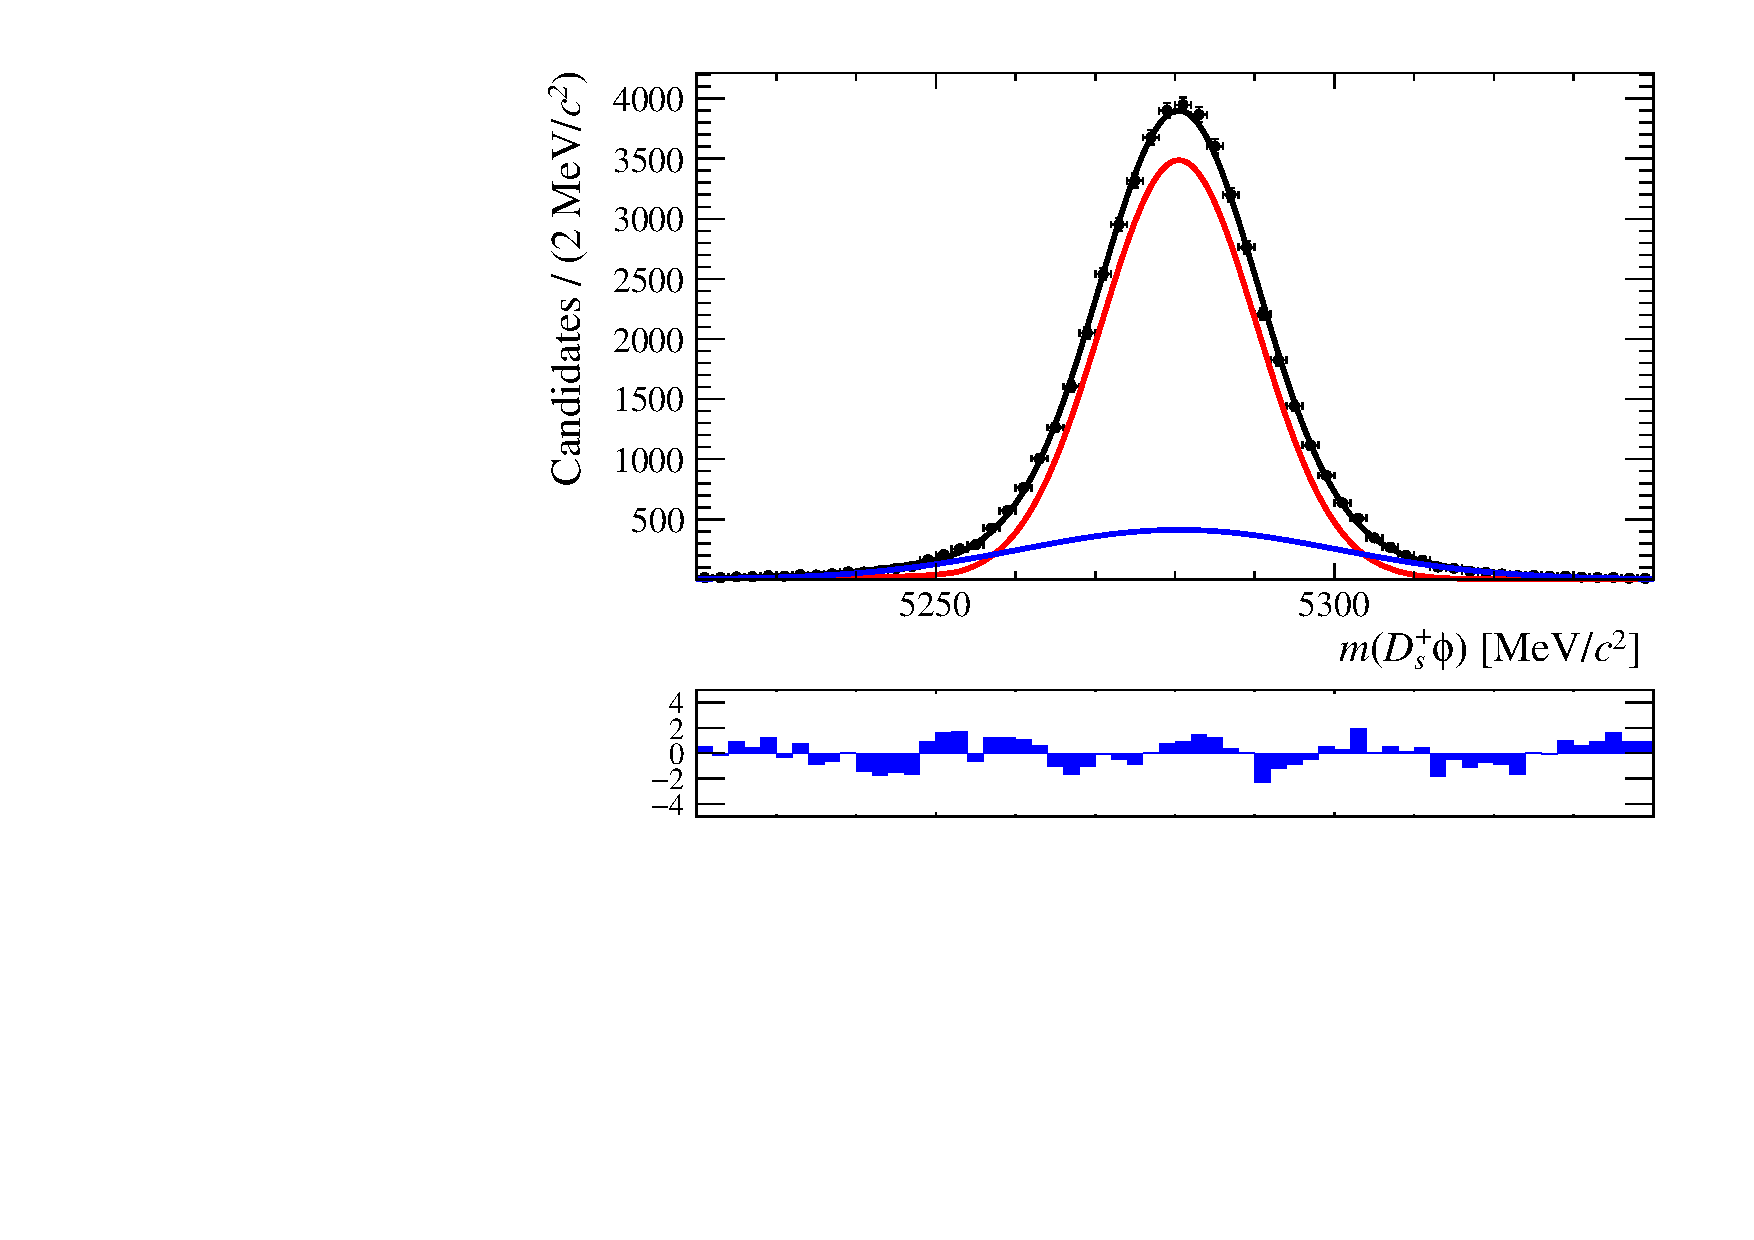
\includegraphics[width=0.40\textwidth]{figs/B2DsPhi/Plot_Signal_Fit_All_B2PhiDs_Ds2KKPi.pdf}
%       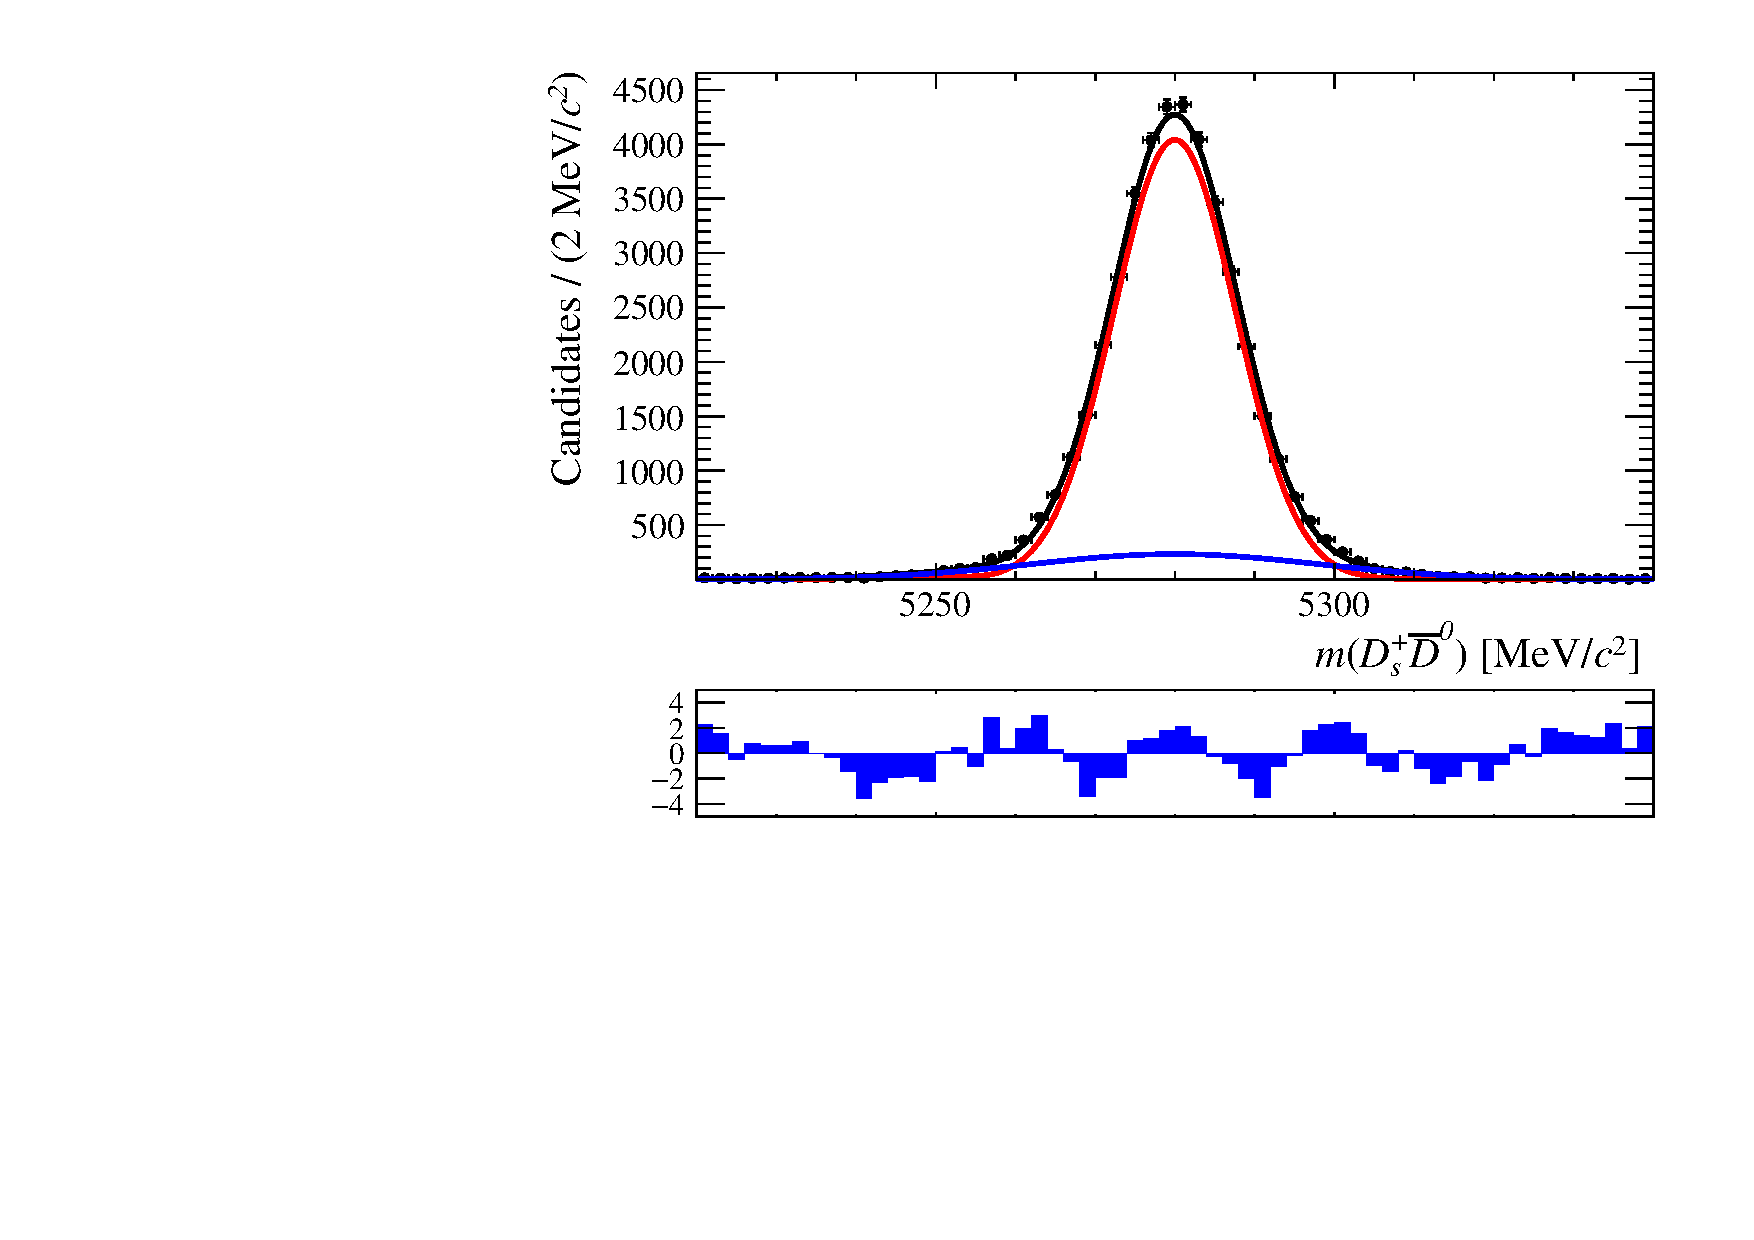
\includegraphics[width=0.40\textwidth]{figs/B2DsPhi/Plot_Signal_Fit_All_B2D0Ds_Ds2KKPi.pdf}
%    \caption{\decay{\Dsp}{\Kp\Km\pip}}
%    \end{subfigure}\\
%    \begin{subfigure}[t]{1.0\textwidth}
%       \centering
%       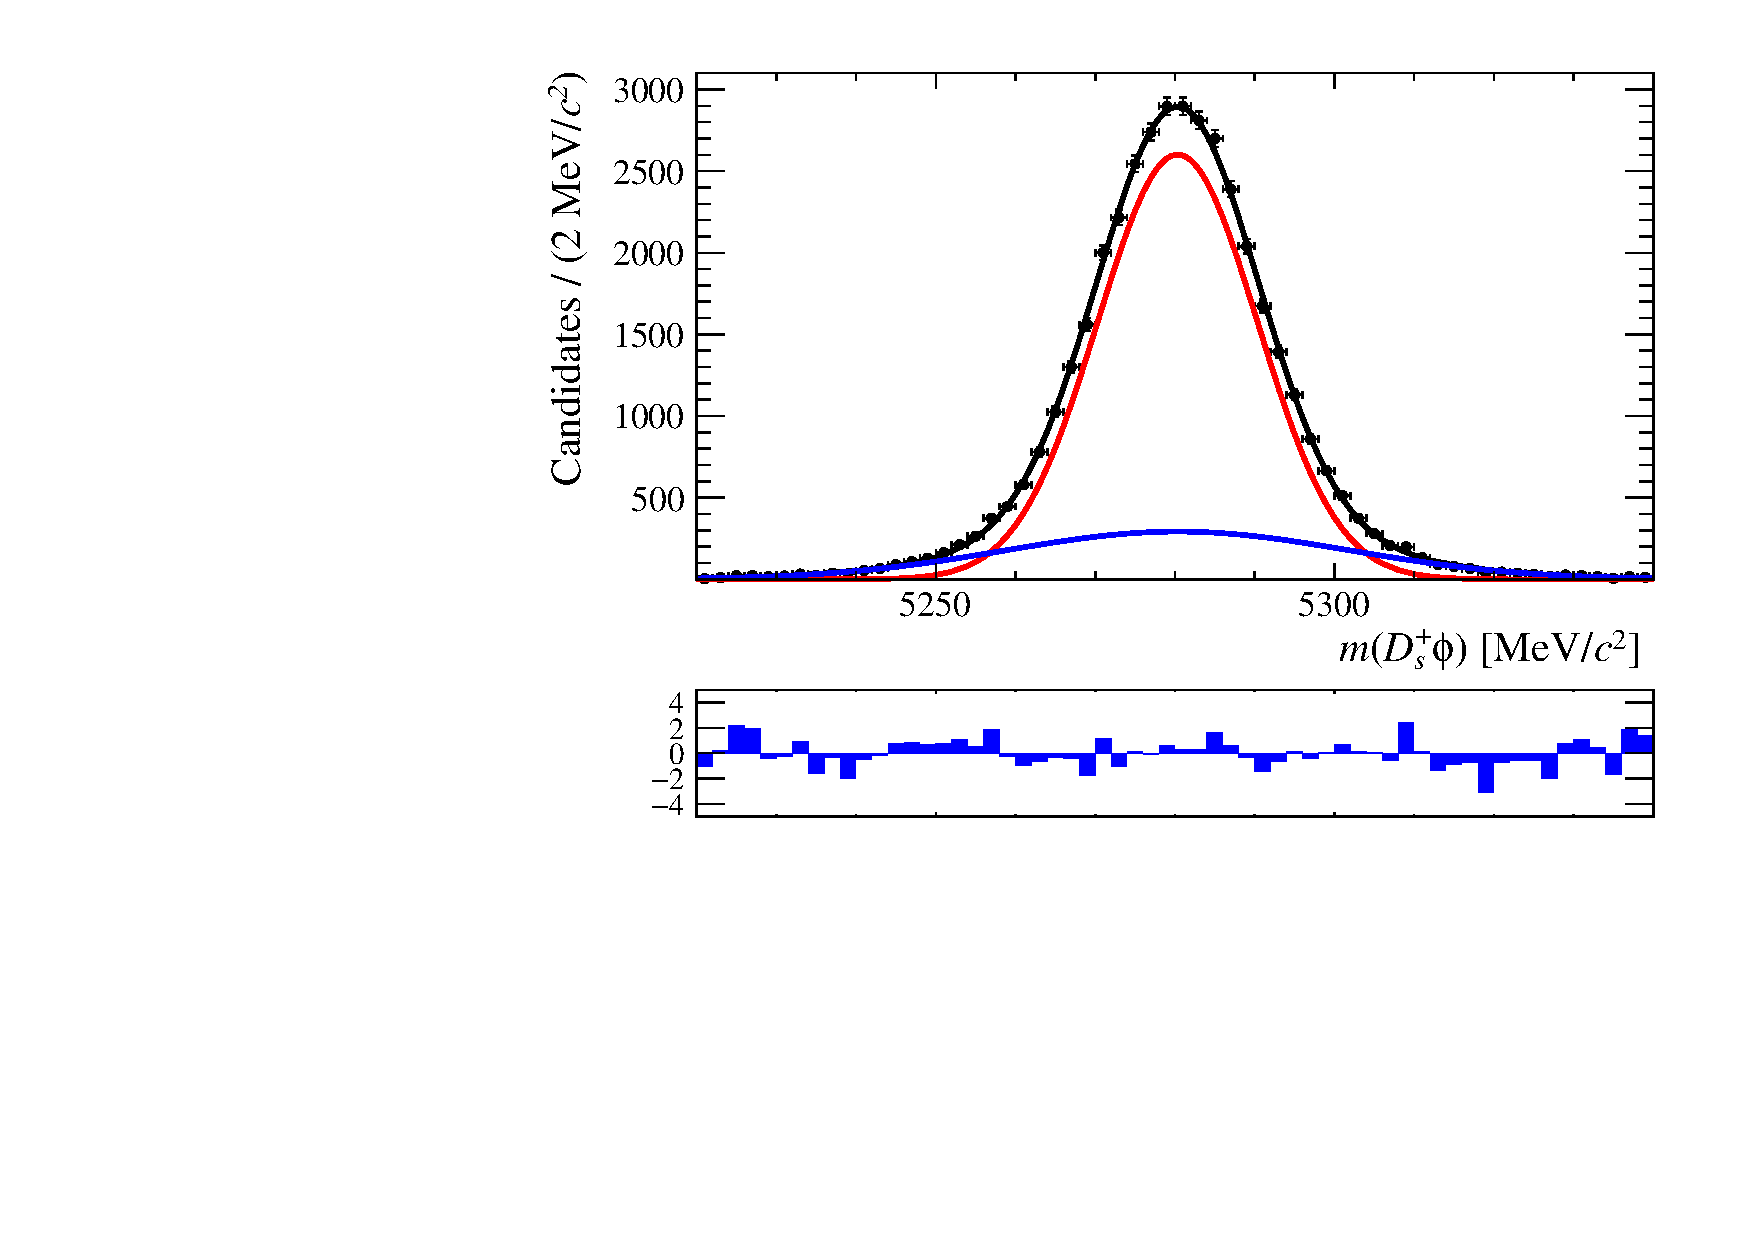
\includegraphics[width=0.40\textwidth]{figs/B2DsPhi/Plot_Signal_Fit_All_B2PhiDs_Ds2PiPiPi.pdf}
%       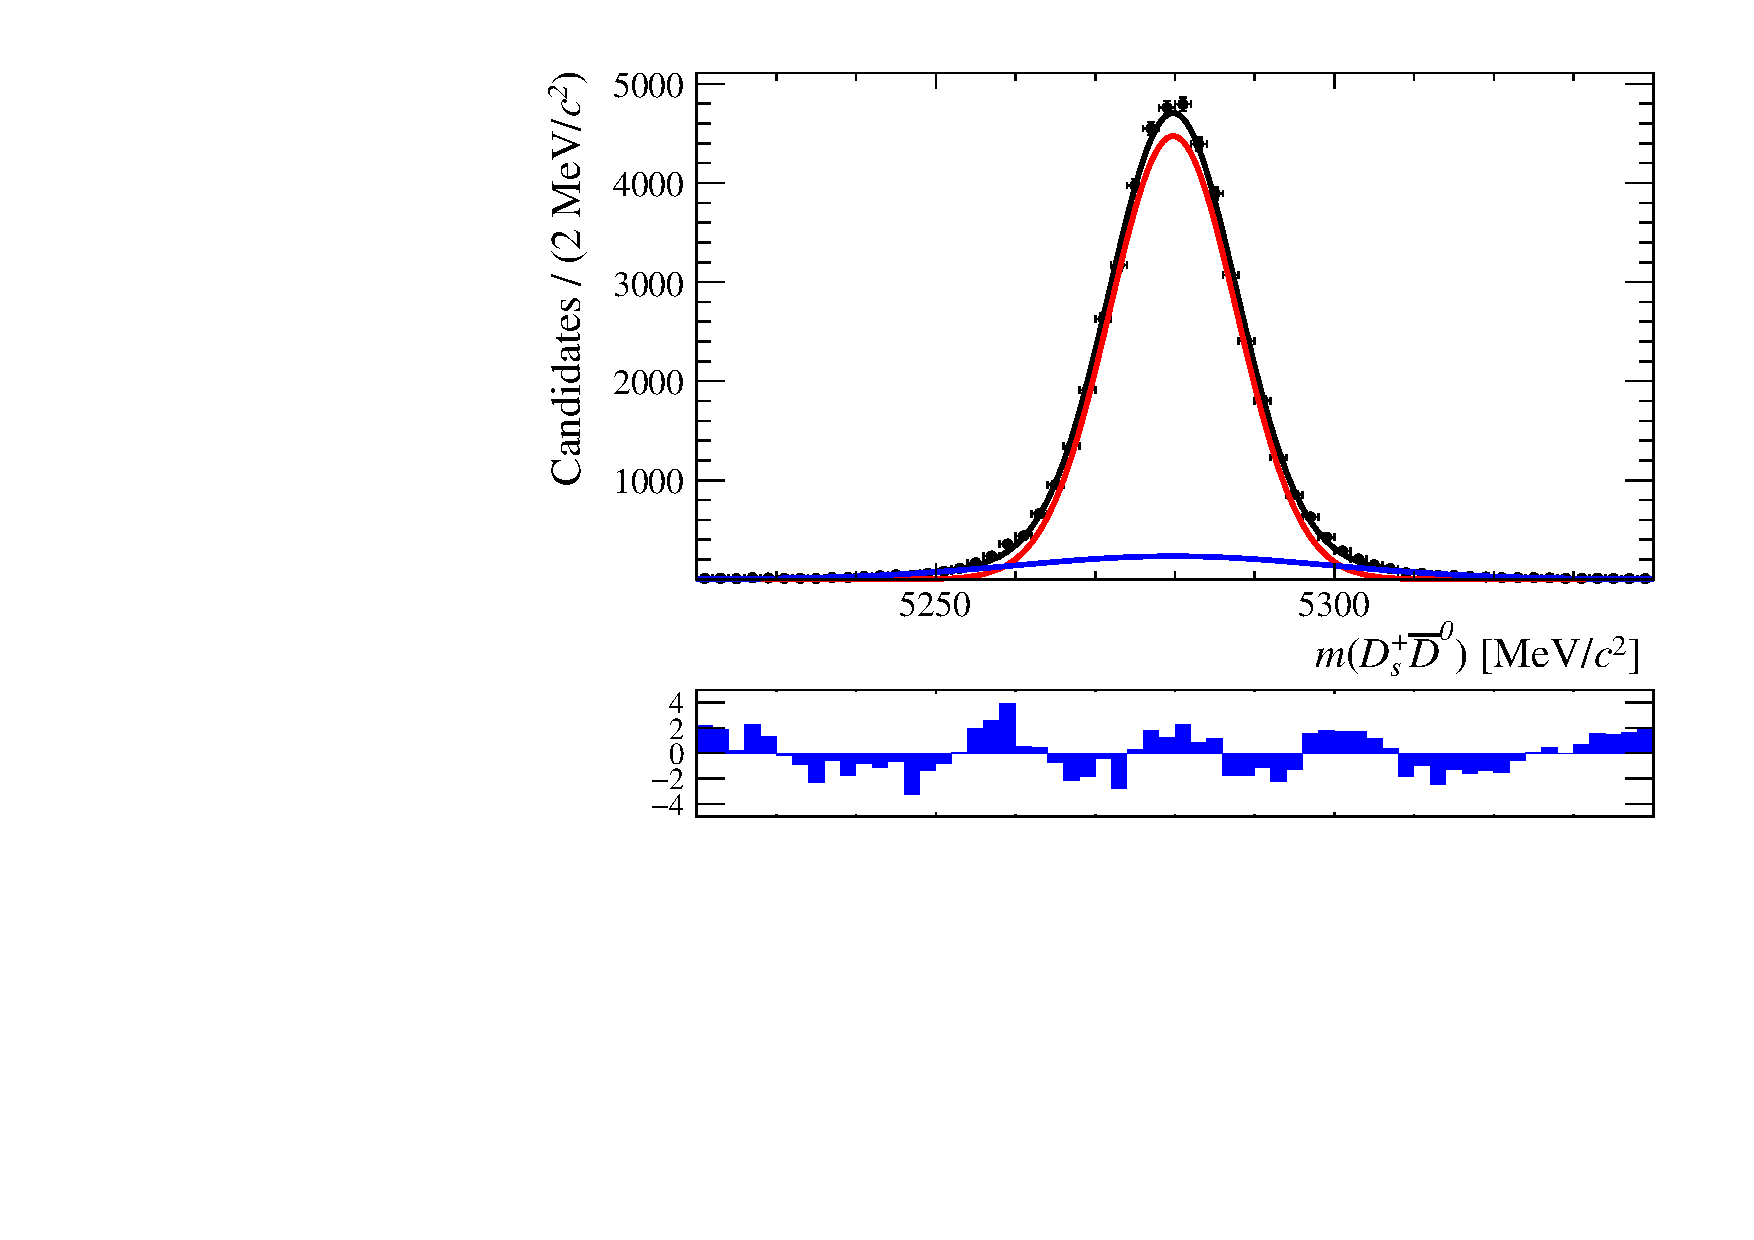
\includegraphics[width=0.40\textwidth]{figs/B2DsPhi/Plot_Signal_Fit_All_B2D0Ds_Ds2PiPiPi.pdf}
%       \caption{\decay{\Dsp}{\pip\pim\pip}}
%    \end{subfigure}\\
%    \begin{subfigure}[t]{1.0\textwidth}
%       \centering
%       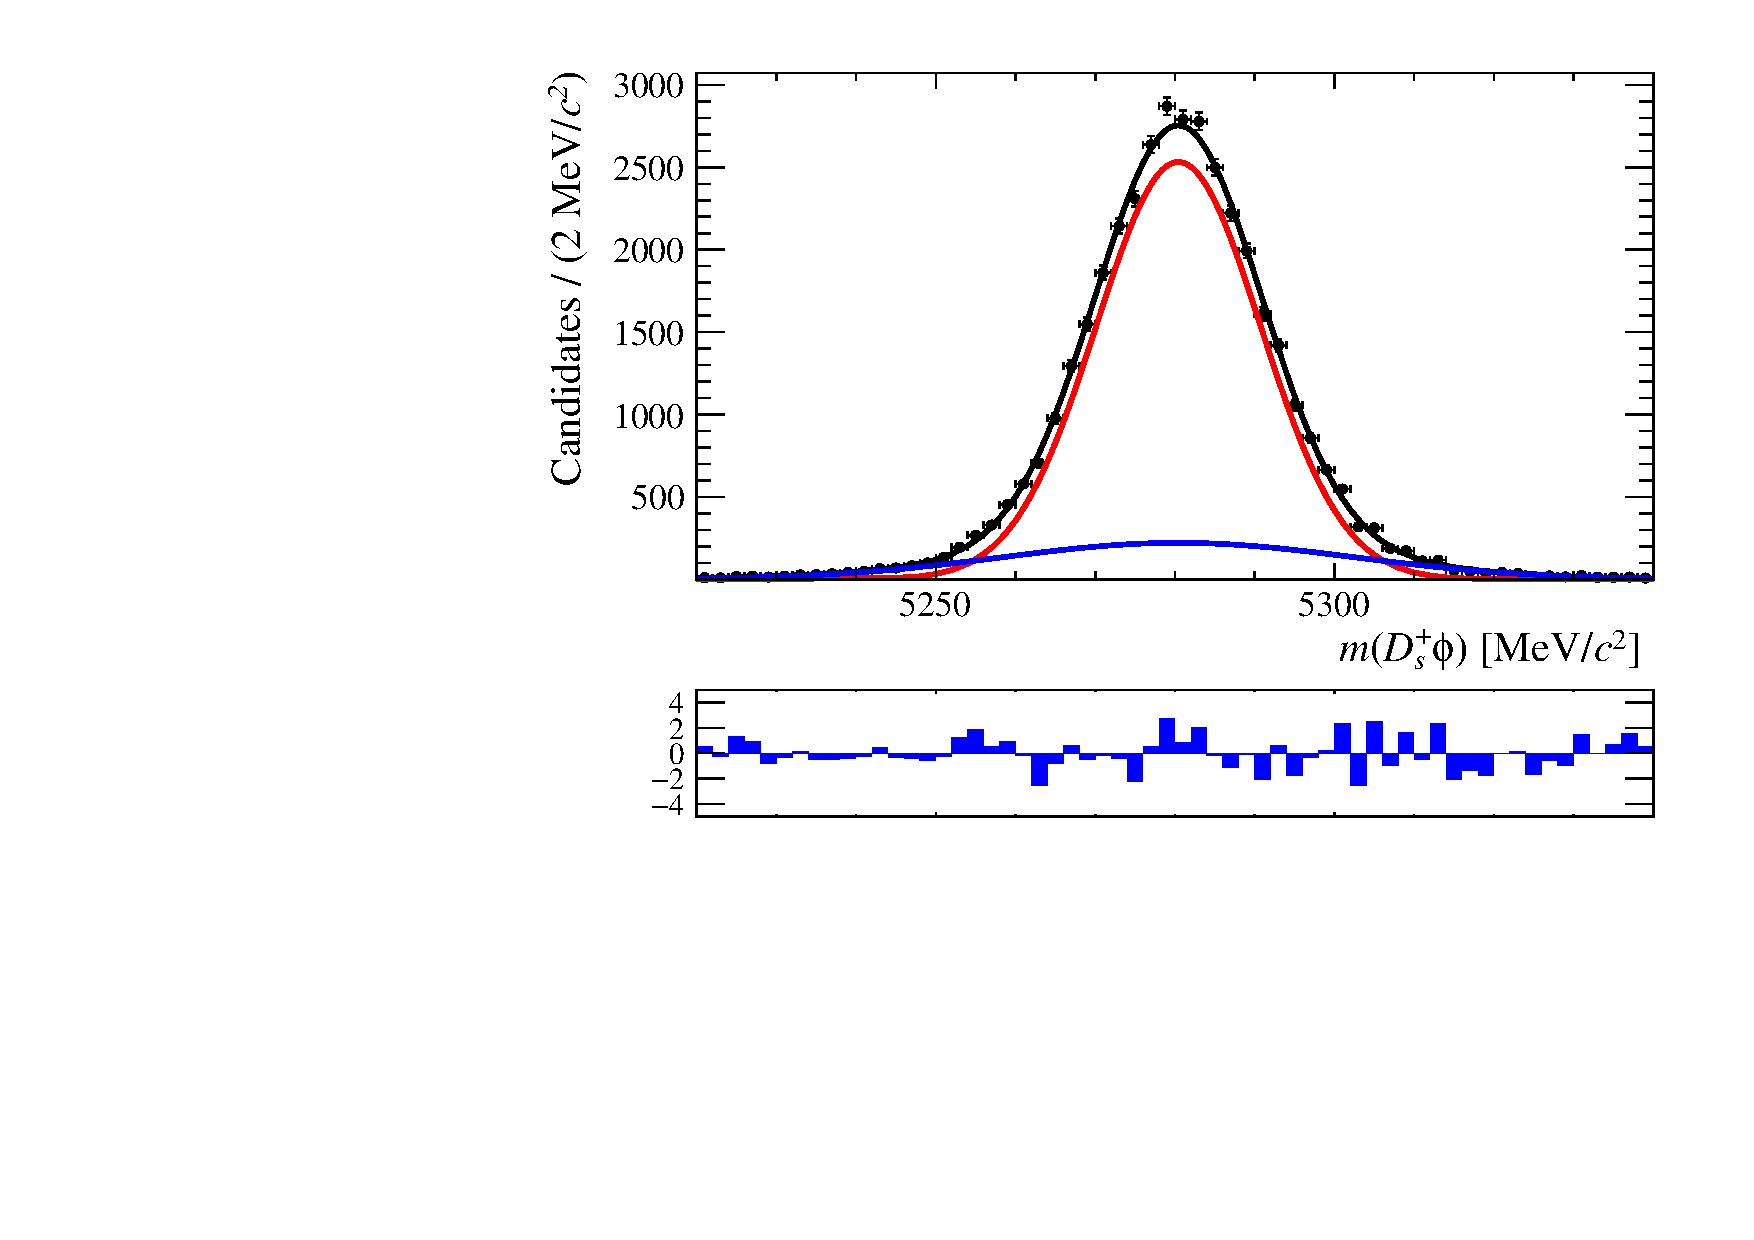
\includegraphics[width=0.40\textwidth]{figs/B2DsPhi/Plot_Signal_Fit_All_B2PhiDs_Ds2KPiPi.pdf}
%       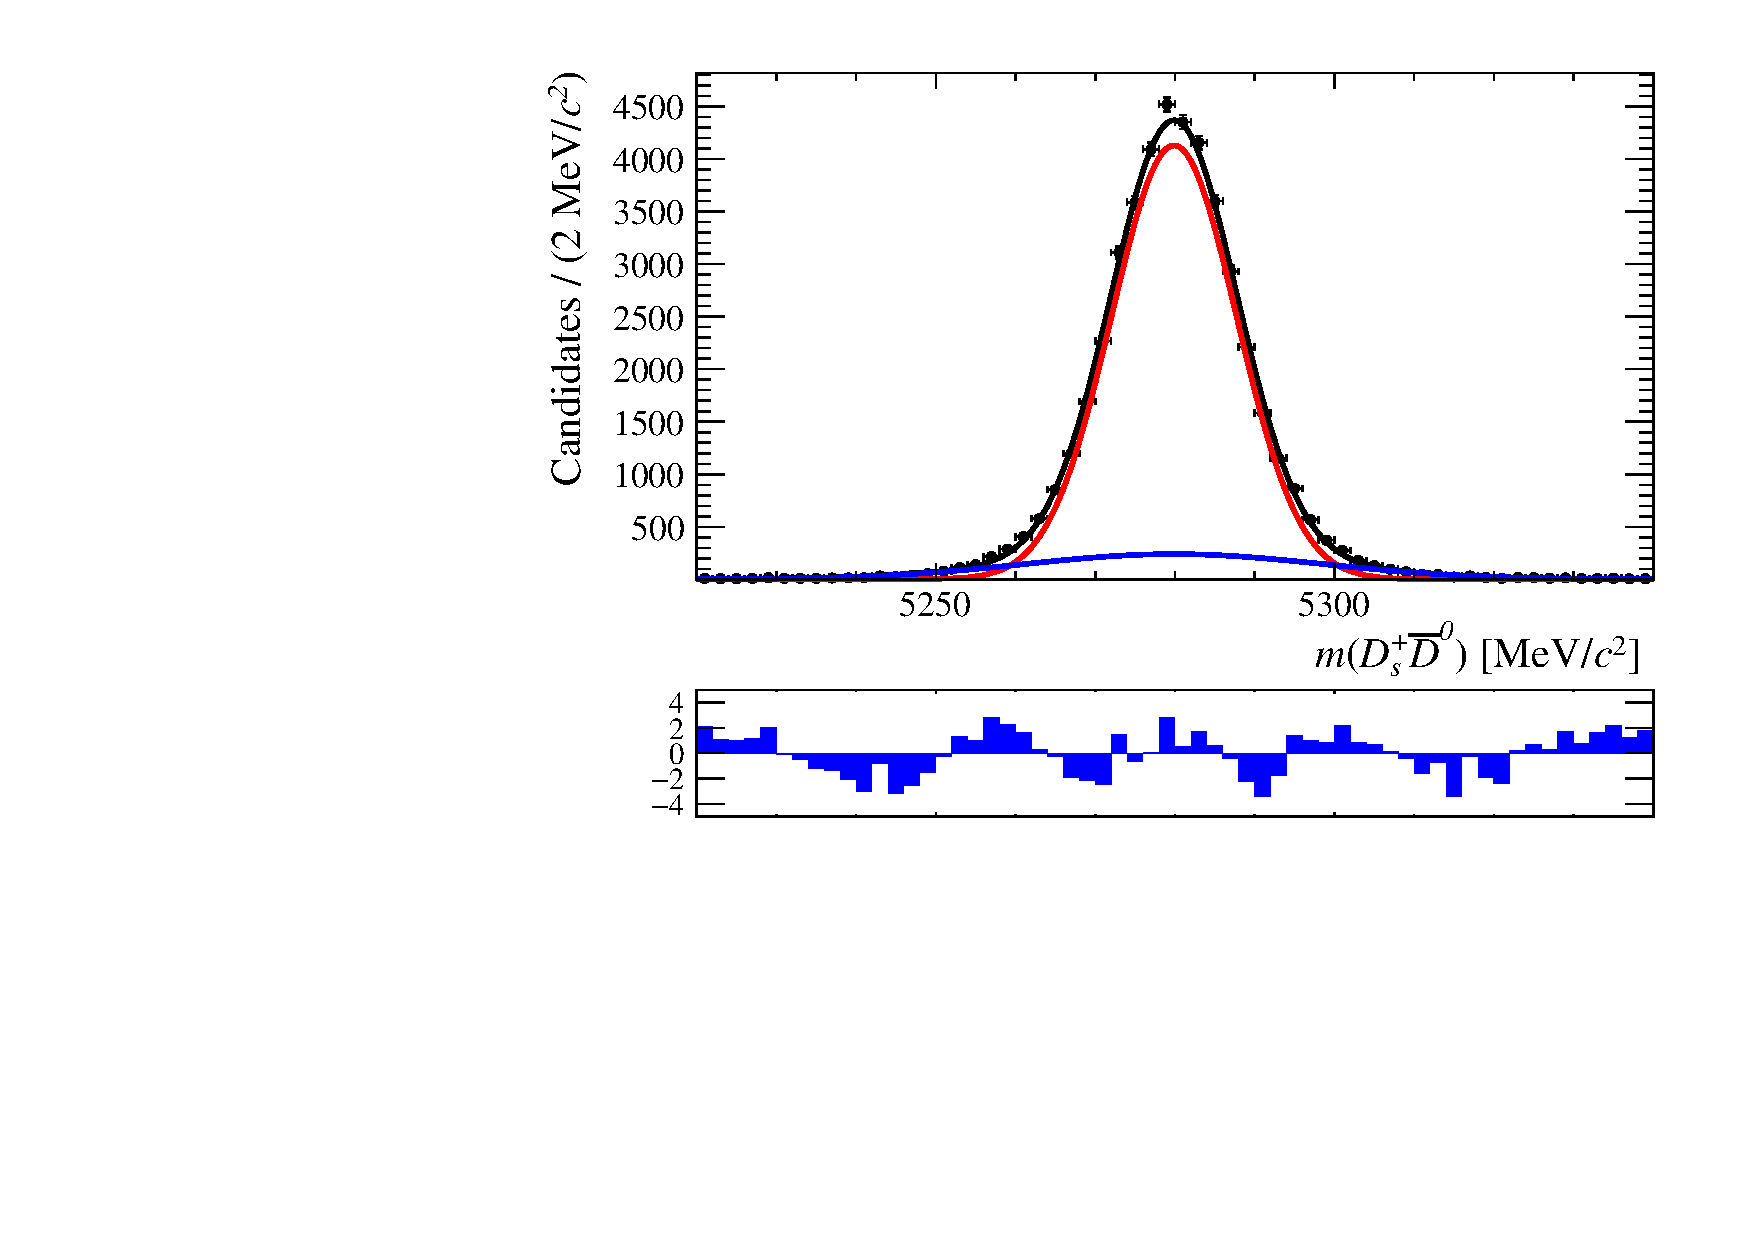
\includegraphics[width=0.40\textwidth]{figs/B2DsPhi/Plot_Signal_Fit_All_B2D0Ds_Ds2KPiPi.pdf}
%       \caption{\decay{\Dsp}{\Kp\pim\pip}}
%    \end{subfigure}\\
%    \caption{Invariant mass fits to simulated signal (left) and normalisation (right) decays. The results of maximum likelihood fits using the signal PDFs are over laid, with the total function in black and the two contributing CB shapes in red and blue.}
%    \label{fig:B2DsPhi_signal_fits}   
% \end{figure}
% %%%%%%%%%%%%%%%%%%%%%%%%%%%%%%%%%%%%%%%%%%%%%%%%%%%%%%%%%%


\subsection{Partially reconstructed backgrounds}
\label{sec:B2DsPhi_partrecocomps}

The accurate parametrisation of partially reconstructed backgrounds is particularly important in the search for \decay{\Bp}{\Dsp\phiz} decays as many different processes contribute to the low invariant mass range of the $m(\Dsp\phiz)$ spectrum. These processes involve decays of \Bs, \Bz or \Bp mesons in which the five final state tracks reconstructed in the search for \decay{\Bp}{\Dsp\phiz} decays are only a subset of the background modes final state. 
Typically, processes in which a low momentum pion or photon has not been reconstructed are found closest in mass to the signal decays. 

\subsubsection{Backgrounds to the normalisation channel, \decay{\Bp}{\Dsp\Dzb}}

 \begin{description}
\item \textbf{\decay{\Bp}{(\decay{\Dssp}{\Dsp[\piz/\Pgamma]})\Dzb} and \decay{\Bp}{\Dsp(\decay{\Dstarzb}{\Dzb[\piz/\Pgamma]})}:}
the modes \decay{\Bp}{\Dsp\Dstarzb} and \decay{\Bp}{\Dssp\Dzb} can both contribute as partially reconstructed backgrounds to the \decay{\Bp}{\Dsp\Dzb} normalisation mode. These are parametrised using the same PDFs as in the search for \decay{\Bp}{\Ds\Kp\Km} decays, already described in Sec.~\ref{sec:B2DsKK_norm_partreco}. The PDFs are shown in Fig.~\ref{fig:B2DsPhi_DsD0_partreco}.
\end{description}

% \begin{description}
% \item \textbf{\decay{\Bp}{(\decay{\Dssp}{\Dsp[\piz]})\Dzb} and \decay{\Bp}{\Dsp(\decay{\Dstarzb}{\Dzb[\piz]})}:} these components are modelled by a parabola convolved with a resolution Gaussian. The parabola has a minimum in the centre and doesn't extend beyond endpoints $a$ and $b$
% \begin{equation}
% f(m|a,b,\sigma,\xi, \delta) = \int_{a}^{b}\left(\mu-\frac{a+b}{2}\right)^{2} \left( \frac{1-\xi}{b-a}\mu + \frac{b\xi-a}{b-a} \right) e^{-\frac{-(\mu-(m-\delta))^{2}}{2\sigma^{2}}} d\mu.
% \label{eq:DsPhi_RooHorns}
% \end{equation}
% These components are shown by the black lines in Fig.~\ref{fig:B2DsPhi_DsD0_partreco}.

% \item \textbf{\decay{\Bp}{(\decay{\Dssp}{\Dsp[\Pgamma]})\Dzb} and \decay{\Bp}{\Dsp(\decay{\Dstarzb}{\Dzb[\Pgamma]})}:} these components are modelled by a parabola convolved with a resolution Gaussian. The parabola has a maximum in the centre and doesn't extend beyond endpoints $a$ and $b$
% \begin{equation}
% f(m|a,b,\sigma,\xi, \delta) = \int_{a}^{b} -(\mu-a)(\mu-b)\left( \frac{1-\xi}{b-a}\mu + \frac{b\xi-a}{b-a} \right) e^{-\frac{-(\mu-(m-\delta))^{2}}{2\sigma^{2}}} d\mu.
% \label{eq:DsPhi_RooHills}
% \end{equation}
% These components are shown by the blue lines in Fig.~\ref{fig:B2DsPhi_DsD0_partreco}.
% \end{description}

%%%%%%%%%%%%%%%%%%%%%%%%%%%%%%%%%%%%%%%%%%%%%%%%%%%%%%%%%%
\begin{figure}[!h]
    \centering
    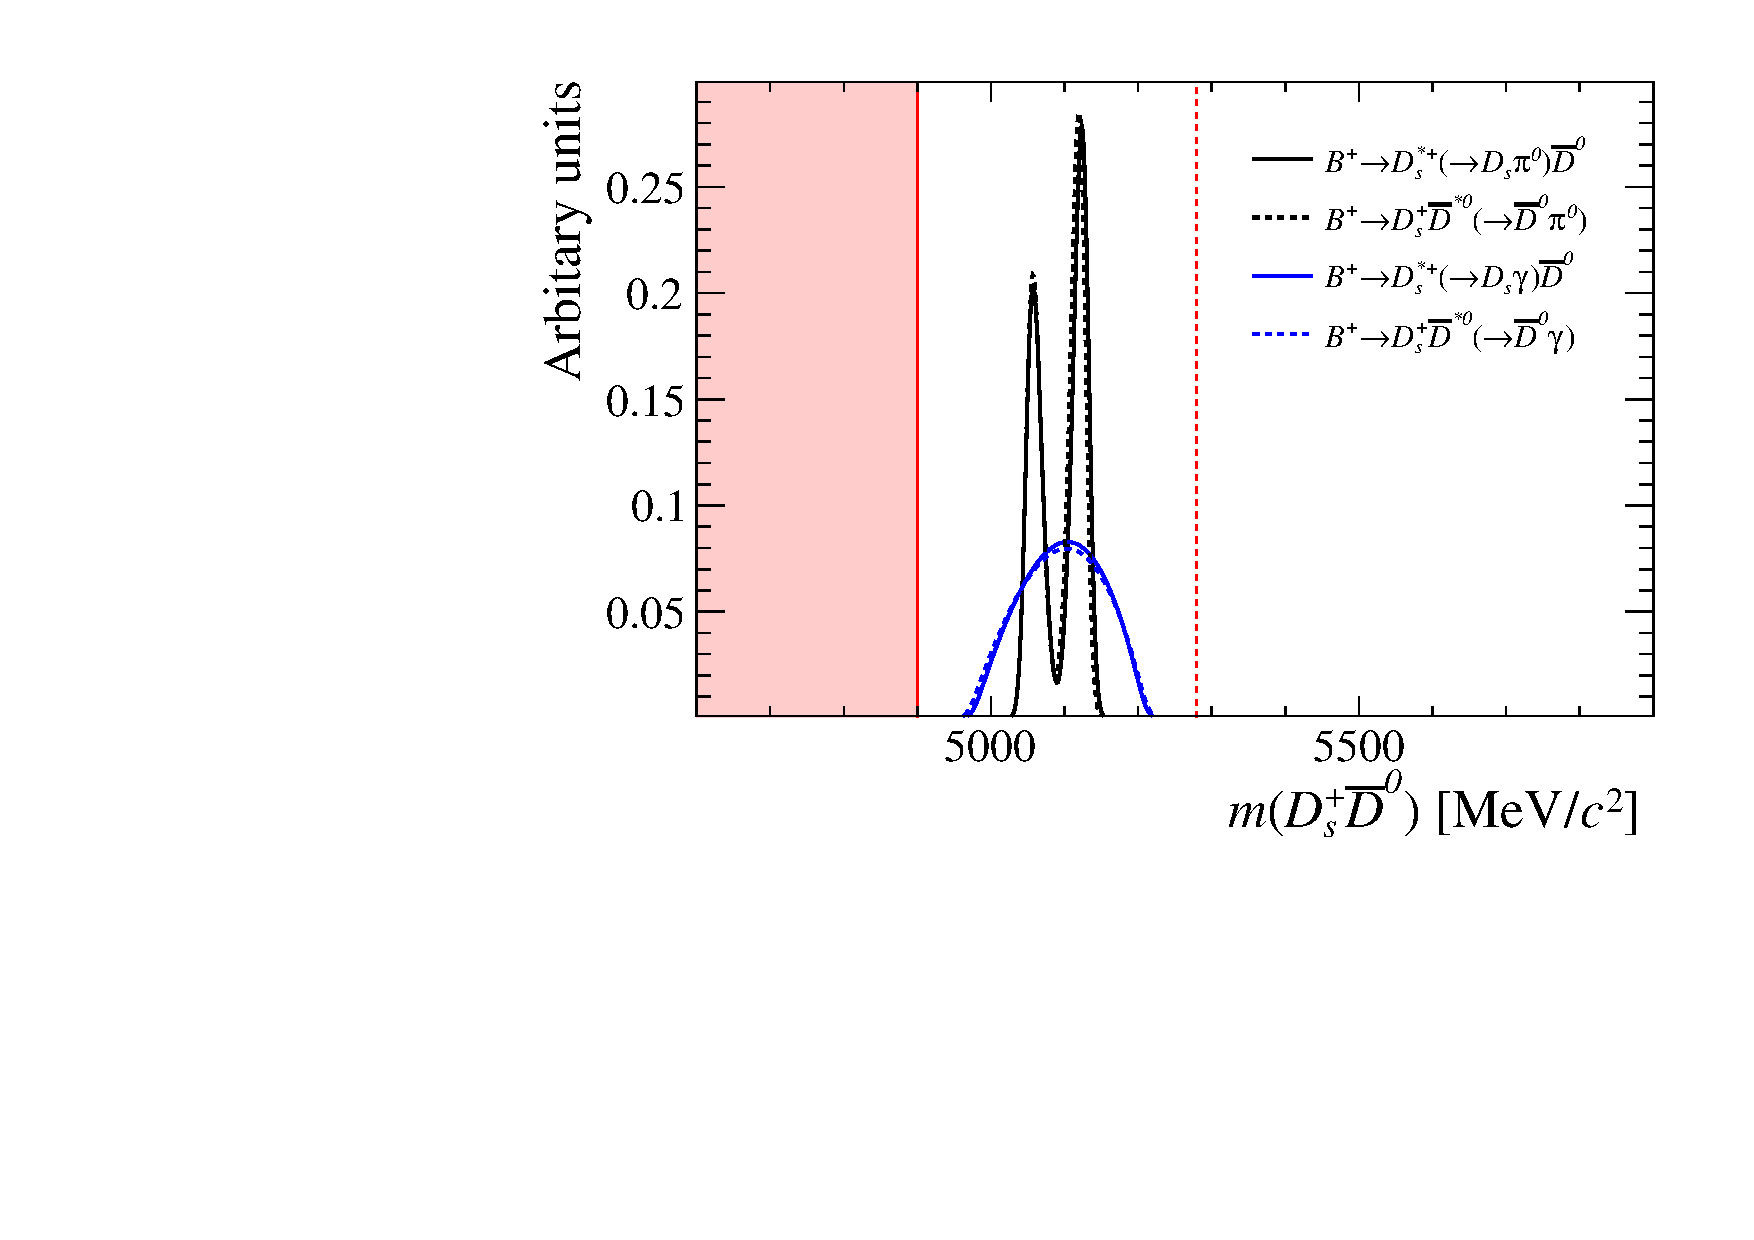
\includegraphics[width=0.70\textwidth]{figs/B2DsPhi/DsD0_part_reco_Shapes.pdf}
    \caption{Partially reconstructed \decay{\Bp}{\Dsp\Dstarzb} and \decay{\Bp}{\Dssp\Dzb} decay parametrisations. The \Bp mass is represented by a vertical dashed red line. Candidates in the area below 4900\mevcc are not included in the fit.}
    \label{fig:B2DsPhi_DsD0_partreco}   
\end{figure}
%%%%%%%%%%%%%%%%%%%%%%%%%%%%%%%%%%%%%%%%%%%%%%%%%%%%%%%%%%

%The invariant mass fit range is wider than in the fit to \decay{\Bp}{\Dsp\Kp\Km} candidates, therefore an extra contribution is included in the fit model to account for partially reconstructed \decay{\Bp}{\Dssp\Dstarzb} decays at lower invariant masses.

\begin{description}

\item \textbf{\decay{\Bp}{\Dssp\Dstarzb}:} the lower invariant mass range used in this search necessitates including a PDF for \decay{\Bp}{\Dssp\Dstarzb} decays in which two soft particles have been missed, one from each of the excited \D meson decays. It is possible for either a \piz or \Pgamma to be not reconstructed in the decays of both excited \D mesons. Additionally, as this process involves a psecudo-scalar meson decaying to two vector mesons, there should be two distinguishable helicity combinations for each process. This leads to a total of eight PDFs necessary to fully parametrise this contribution. Instead, however, this component is parametrised using a single function of the form given in Eq.~\ref{eq:DsPhi_RooHills}. The endpoints $a$ and $b$ are estimated by combining the effects of missing two neutral particles. The resulting distribution is shown in Fig.~\ref{fig:B2DsPhi_DsstarDstar0_partreco}.
The choice of PDF for this component is found to have negligible effect on the determination of the $\BF(\decay{\Bp}{\Dsp\phiz})$ branching fraction as detailed in Sec~\ref{sec:B2DsPhi_systuncertainy}.

\end{description}

%%%%%%%%%%%%%%%%%%%%%%%%%%%%%%%%%%%%%%%%%%%%%%%%%%%%%%%%%%
\begin{figure}[!h]
    \centering
    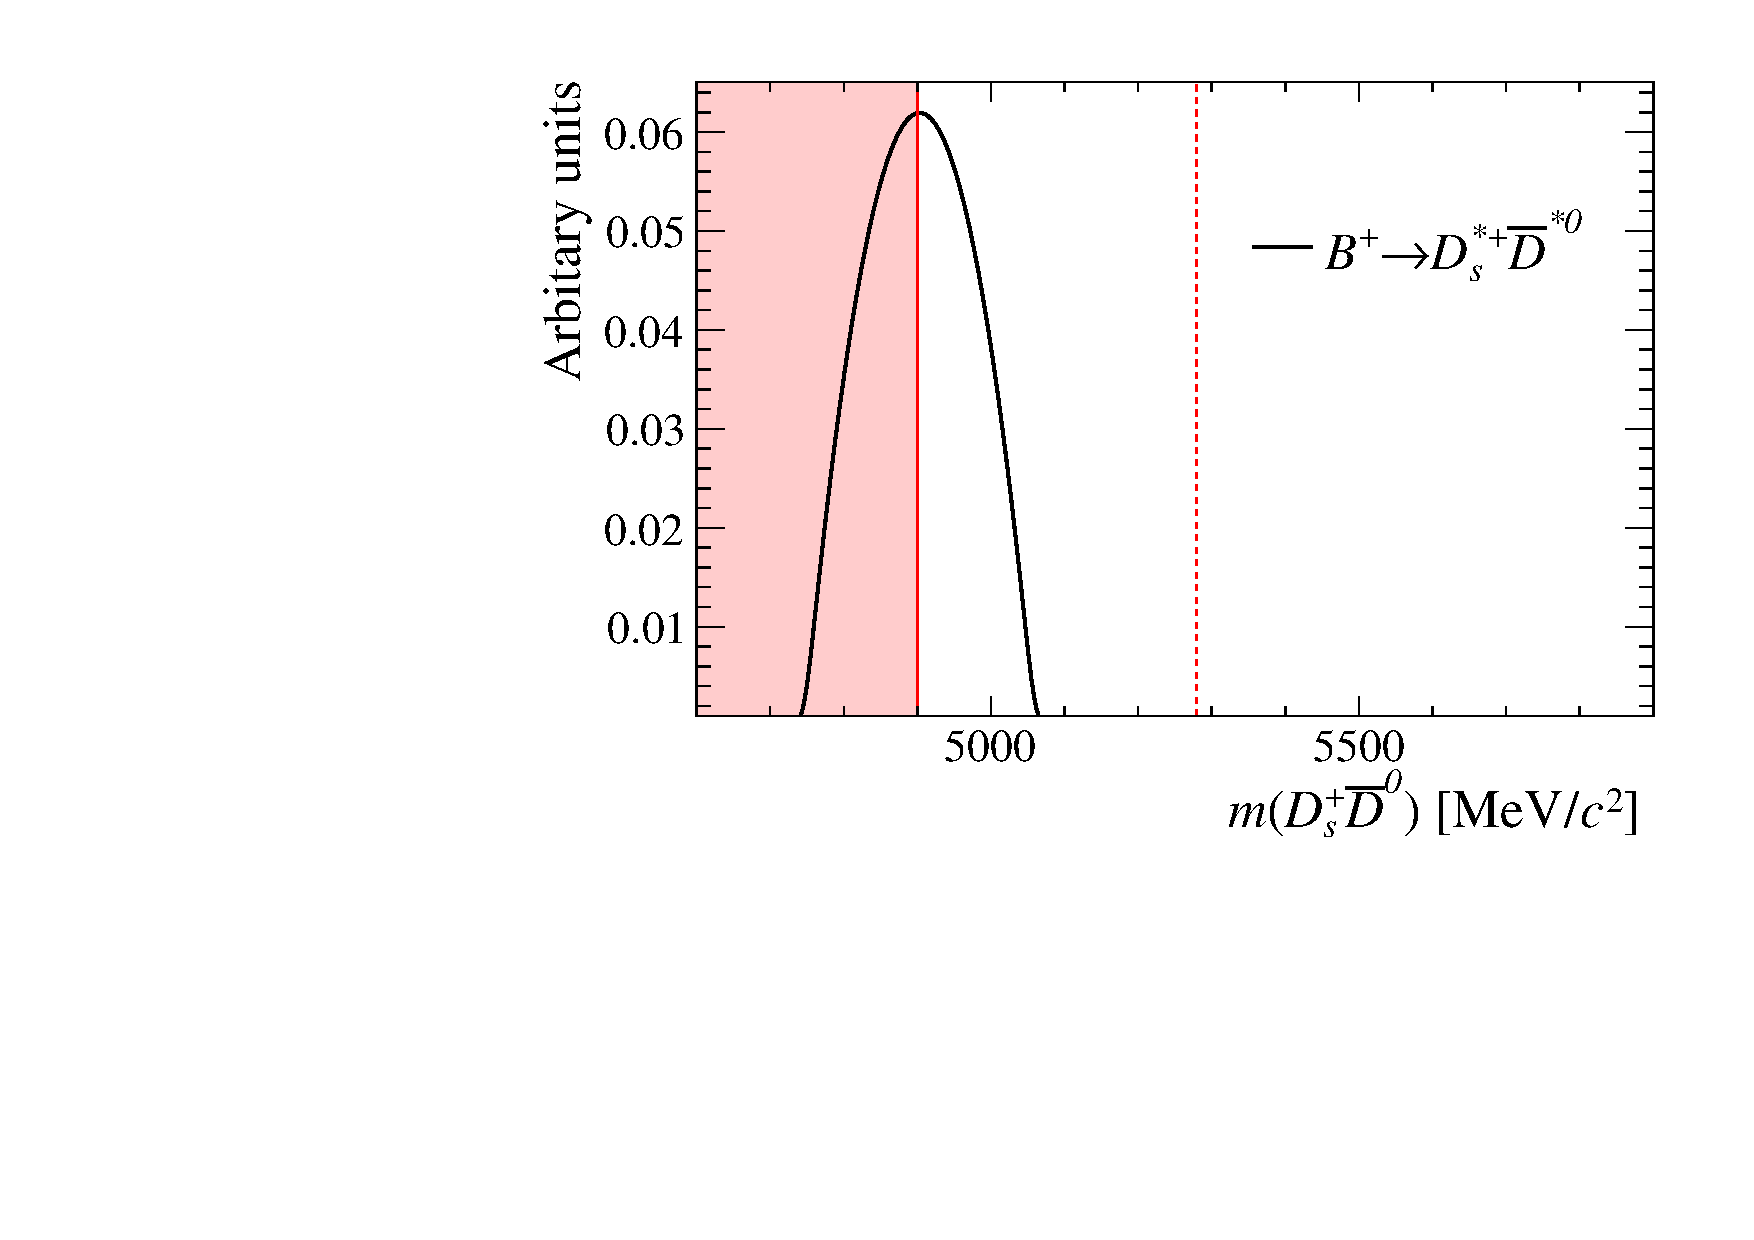
\includegraphics[width=0.70\textwidth]{figs/B2DsPhi/DsstarDstar0_part_reco_Shapes.pdf}
    \caption{Partially reconstructed \decay{\Bp}{\Dssp\Dstarzb} decay parametrisation. The PDF extends below the lower fit range at 4900\mevcc.}
    \label{fig:B2DsPhi_DsstarDstar0_partreco}   
\end{figure}
%%%%%%%%%%%%%%%%%%%%%%%%%%%%%%%%%%%%%%%%%%%%%%%%%%%%%%%%%%



\subsubsection{Backgrounds to the signal channel, \decay{\Bp}{\Dsp\phiz}}
\label{sec:B2DsPhi_part_recto_sig}
%The signal channel invariant mass distribution receives contributions from the partially reconstructed modes considered in the search for \decay{\Bp}{\Dsp\Kp\Km} decays. The PDFs determined are 

All of the background to the \decay{\Bp}{\Dsp\Kp\Km} channel already discussed Section~\ref{sec:B2DsKK_sig_partreco} are relevant again in the search for \decay{\Bp}{\Dsp\phiz} decays. This includes \decay{\Bsb}{\Dsp\Km\Kstarz}, \decay{\Bsb}{\Dssp\Km\Kstarz}, \decay{\Bsb}{\Dsp\Dsm}, \decay{\Bzb}{\Dsp\Dm} and \decay{\Bsb}{\Dssp\Dsm} decays. The PDFs are determined using one-dimensional kernel estimation from samples of simulated decays passing the signal selection. These PDFs are updates to only include candidates in the appropriate range of $m(\Kp\Km)$ and shown in Figure~\ref{fig:B2DsPhi_part_reco_shapes}. The fraction of each background expected in each of the four $m(\Kp\Km)$ and $\cos\theta_{K}$ categories is determined from the relevant simulations samples.

The branching fractions the three decays \decay{\Bzb}{\Dsp\Dm}, \decay{\Bsb}{\Dsp\Dsm}, and \decay{\Bsb}{\Dssp\Dsm} are measured to be $(7.2 \pm 0.8 ) \times 10^{-3}$, $(4.4 \pm 0.5 ) \times 10^{-3}$ and $(1.37 \pm 0.16 ) \%$ respectively~\cite{PDG2016}. The relative contributions for these three processes are fixed using these branching fractions, estimates of the relative efficiencies for each mode and the production fraction of \Bsb mesons relative to \Bzb mesons, $f_{s}/f_{d}$. This helps to add stability to the fit.


%%%%%%%%%%%%%%%%%%%%%%%%%%%%%%%%%%%%%%%%%%%%%%%%%%%%%%%%%%
\begin{figure}[!h]
    \centering
    \begin{subfigure}[t]{0.49\textwidth}
        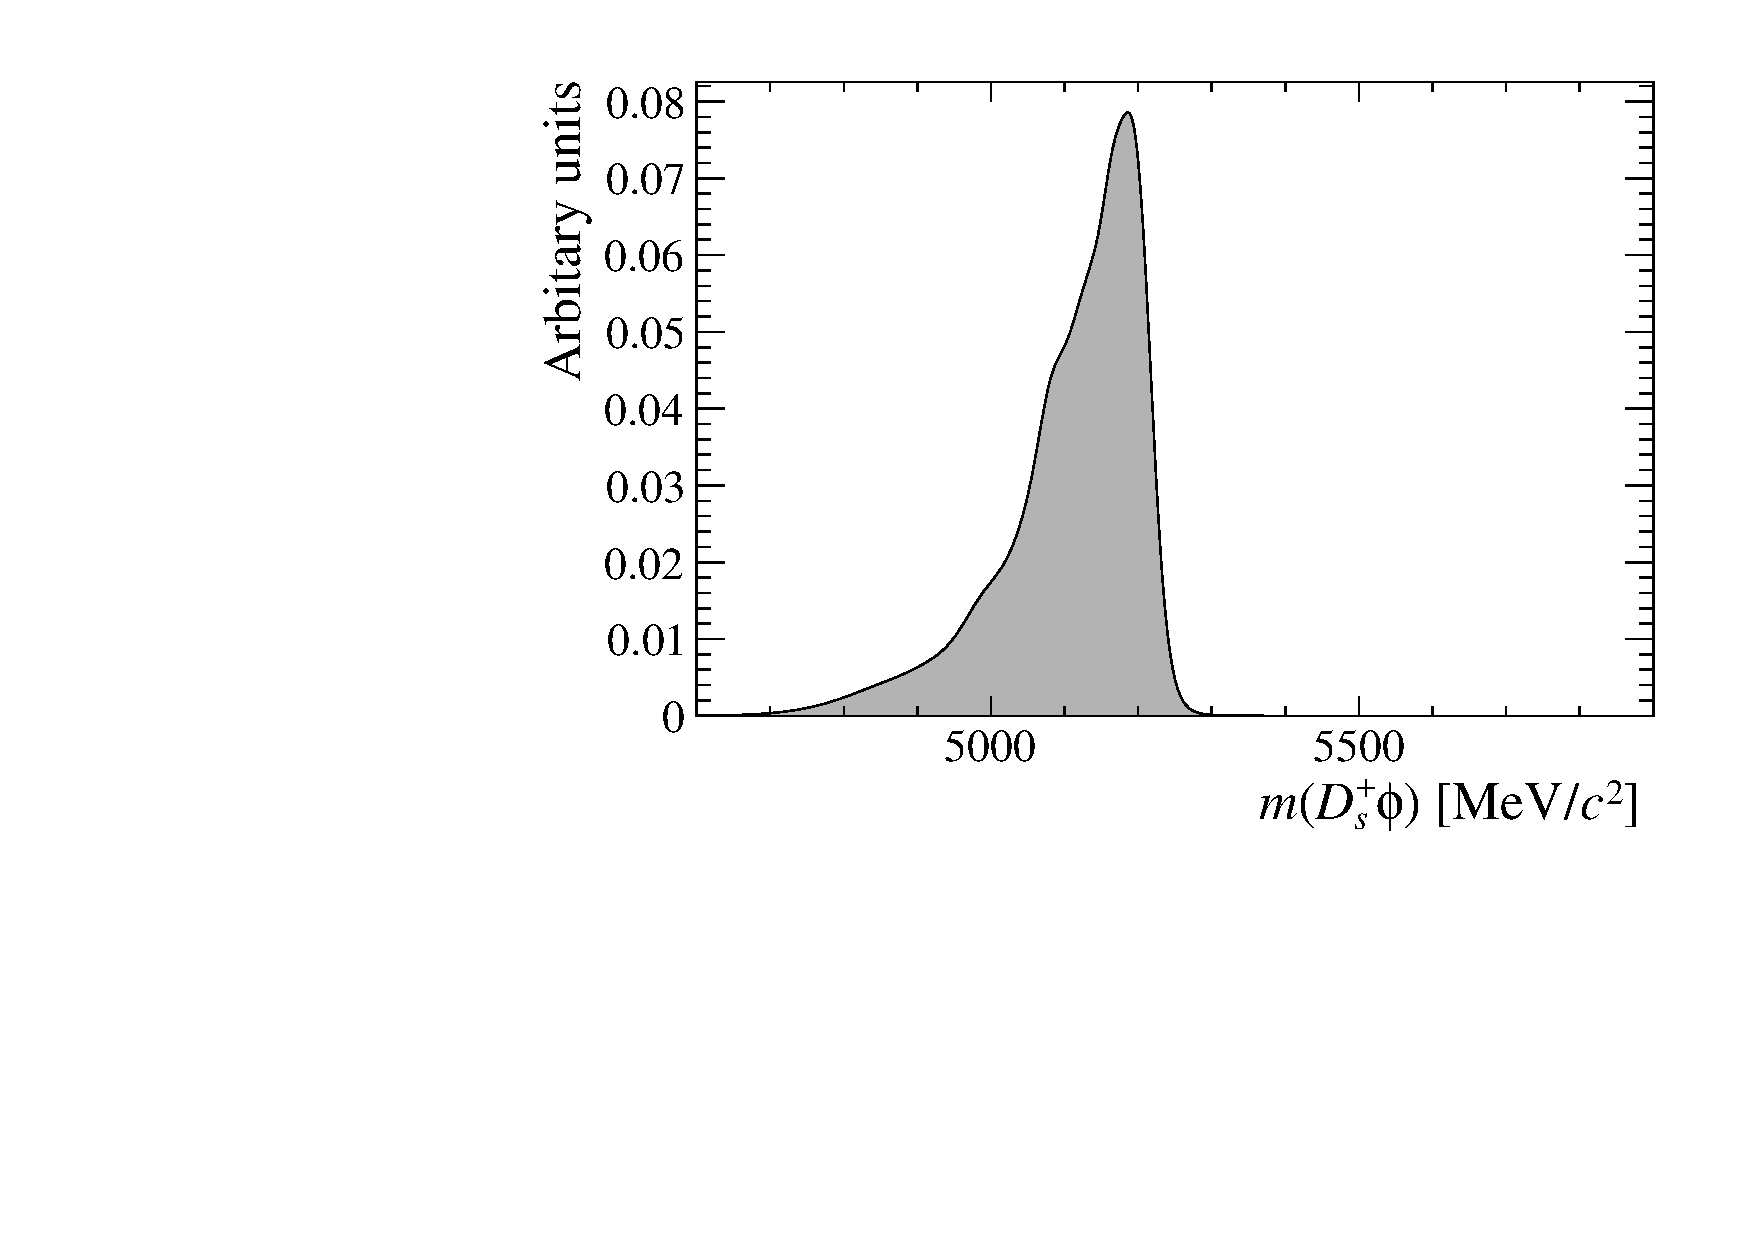
\includegraphics[width=1.0\textwidth]{figs/B2DsPhi/Bs2Dsa1_4600_5900_Shape.pdf}
        \caption{\decay{\Bsb}{\Dsp\Km\Kstarz} }
    \end{subfigure}
    \begin{subfigure}[t]{0.49\textwidth}
        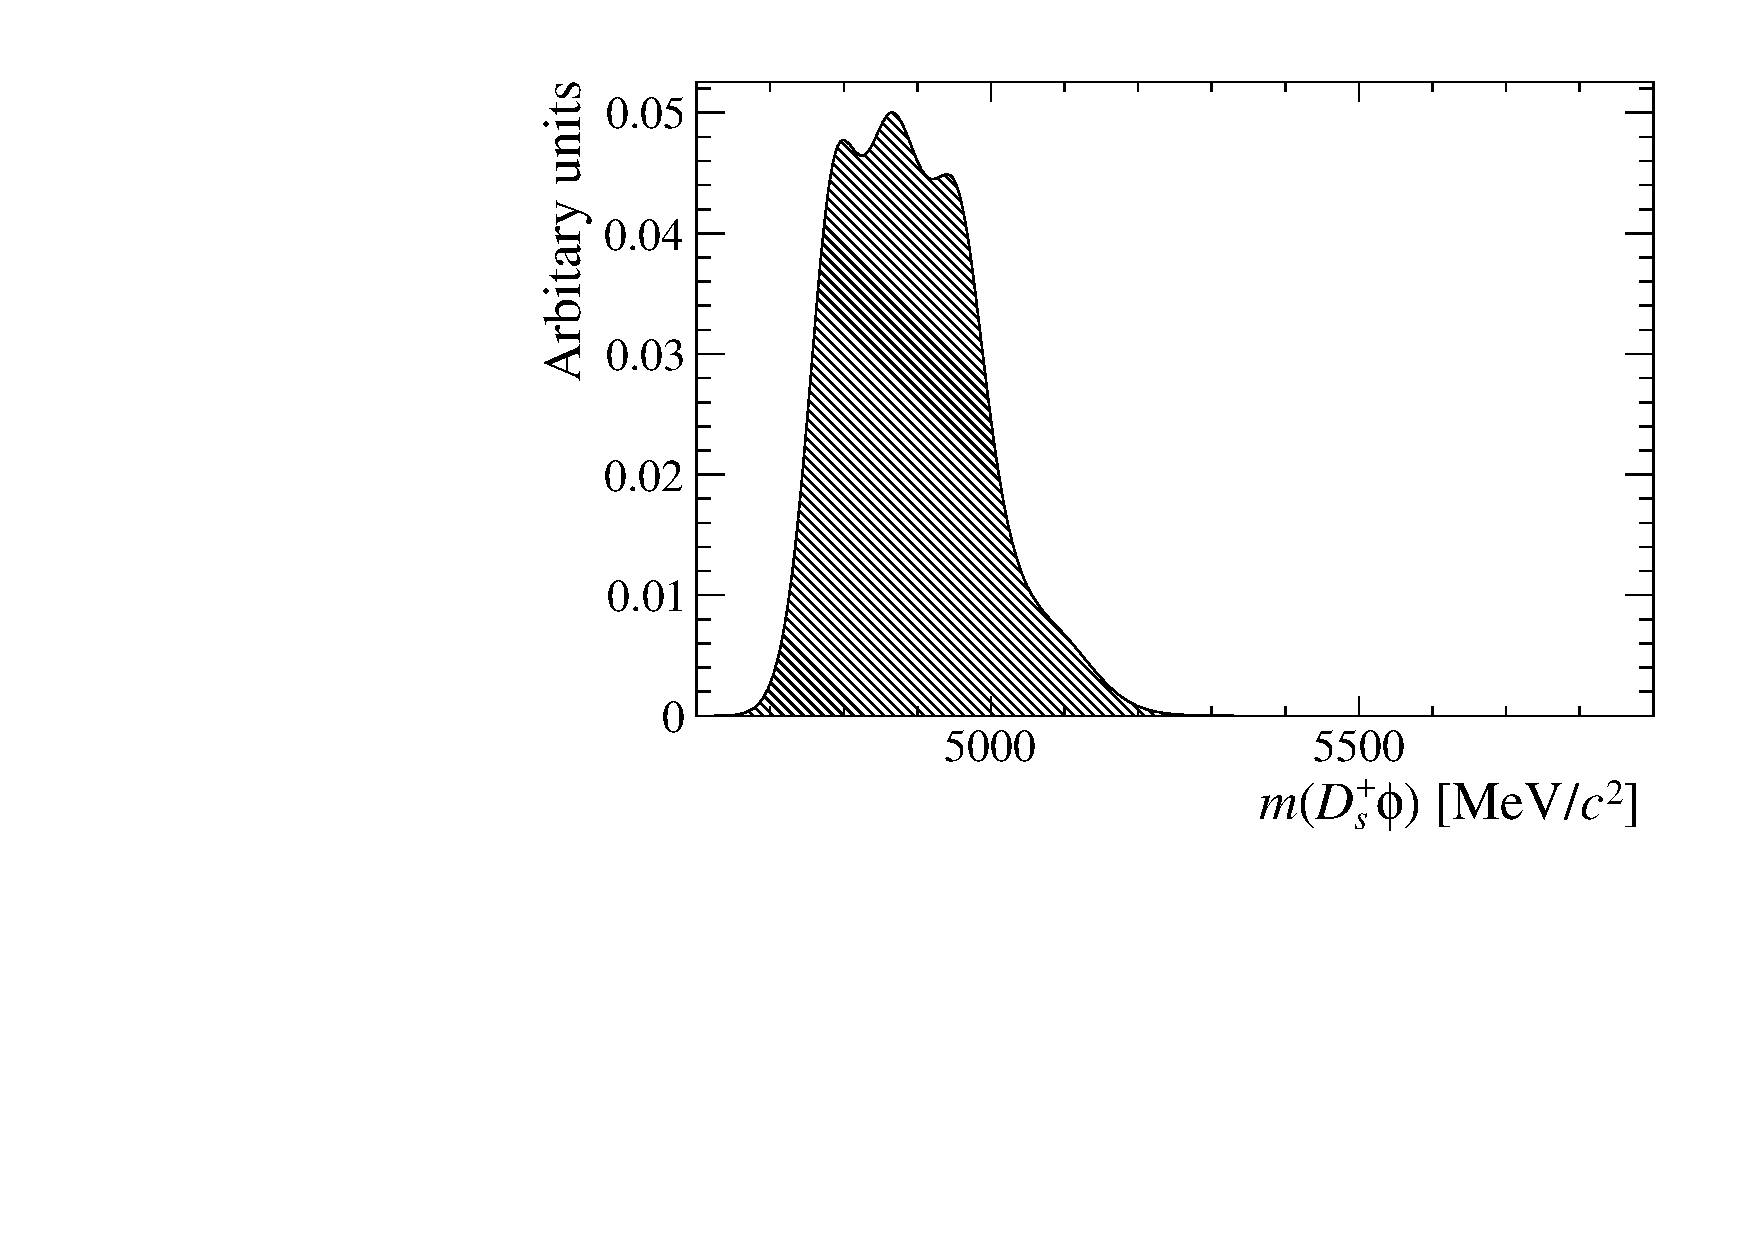
\includegraphics[width=1.0\textwidth]{figs/B2DsPhi/Bs2DsstKKst_4600_5900_Shape.pdf}
        \caption{\decay{\Bsb}{\Dsp\Km\Kstarz} }
    \end{subfigure}
    \begin{subfigure}[t]{0.49\textwidth}
        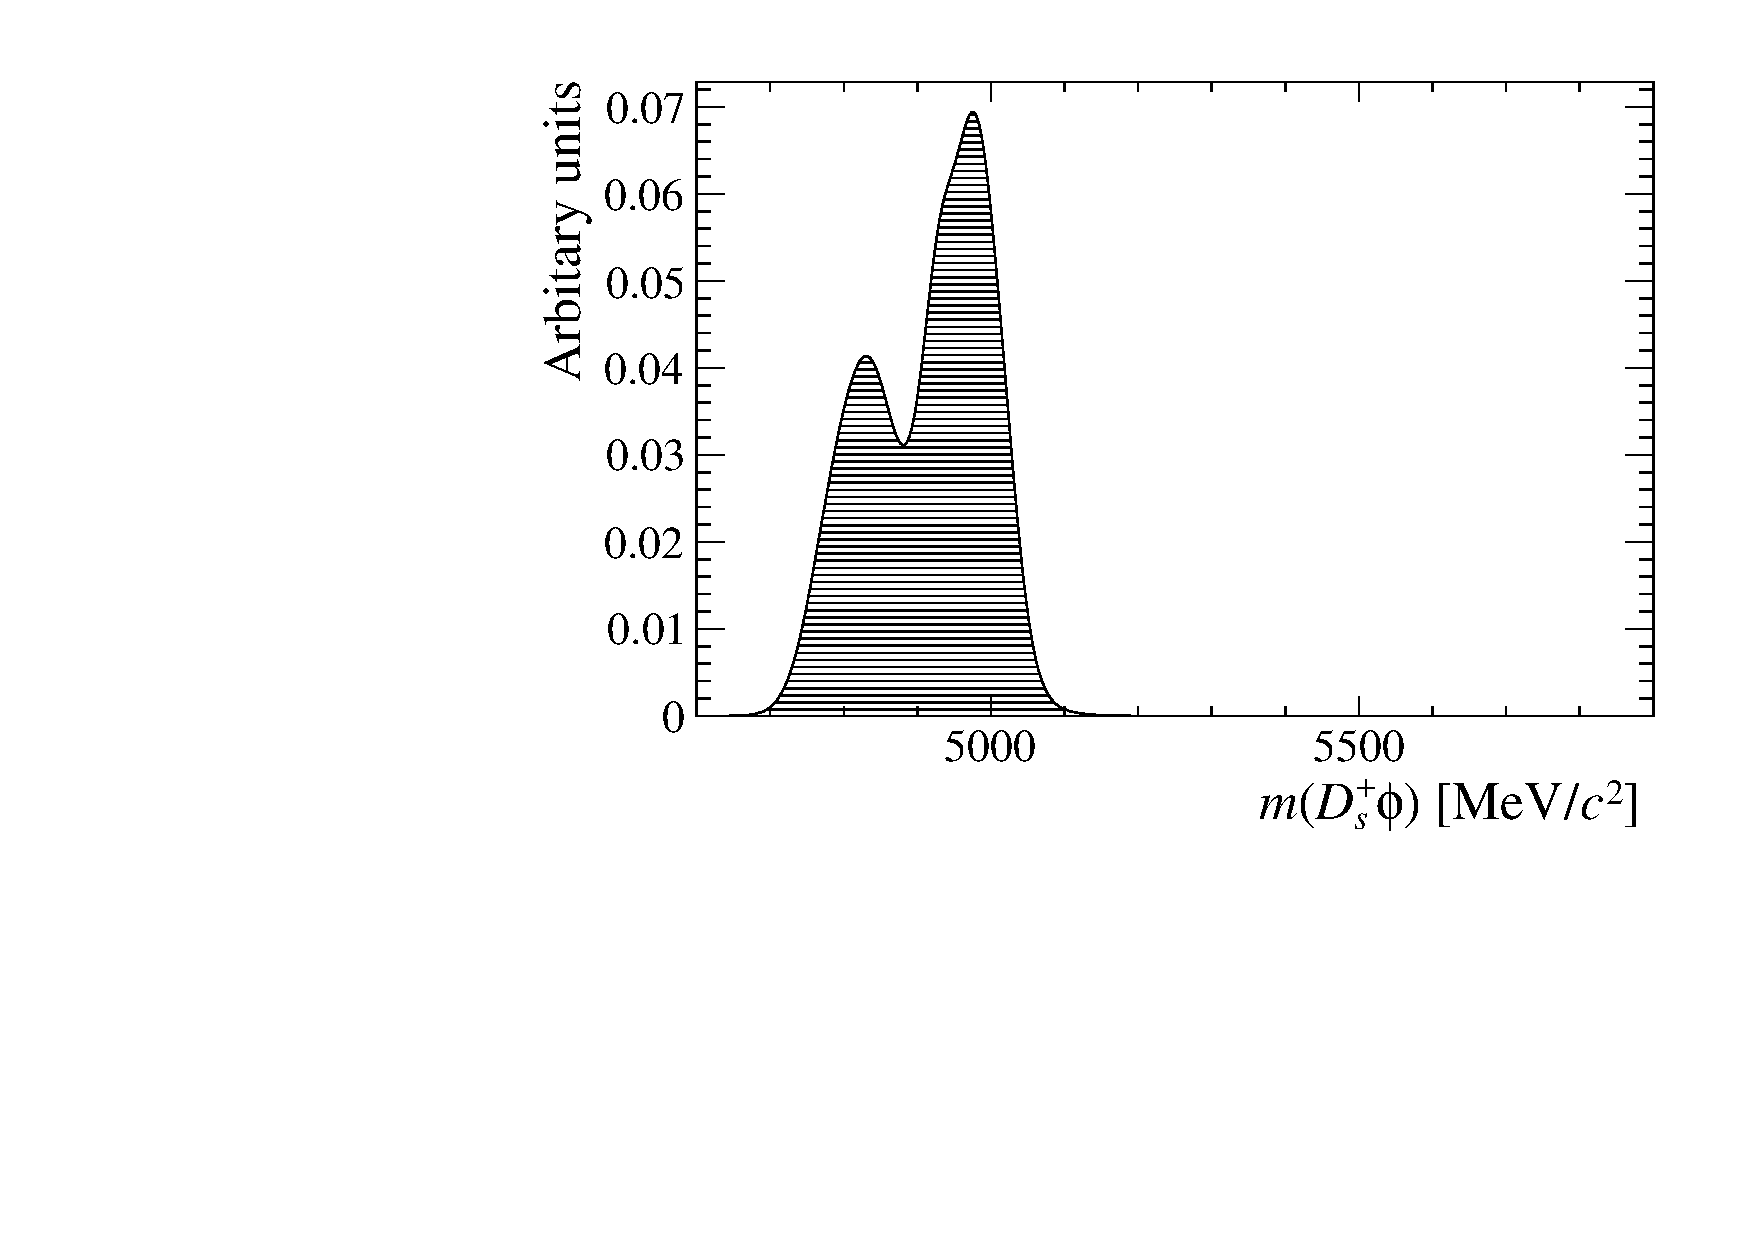
\includegraphics[width=1.0\textwidth]{figs/B2DsPhi/Bs2DsDs_4600_5900_Shape.pdf}
        \caption{\decay{\Bsb}{\Dsp\Dsm} }
    \end{subfigure}
    \begin{subfigure}[t]{0.49\textwidth}
        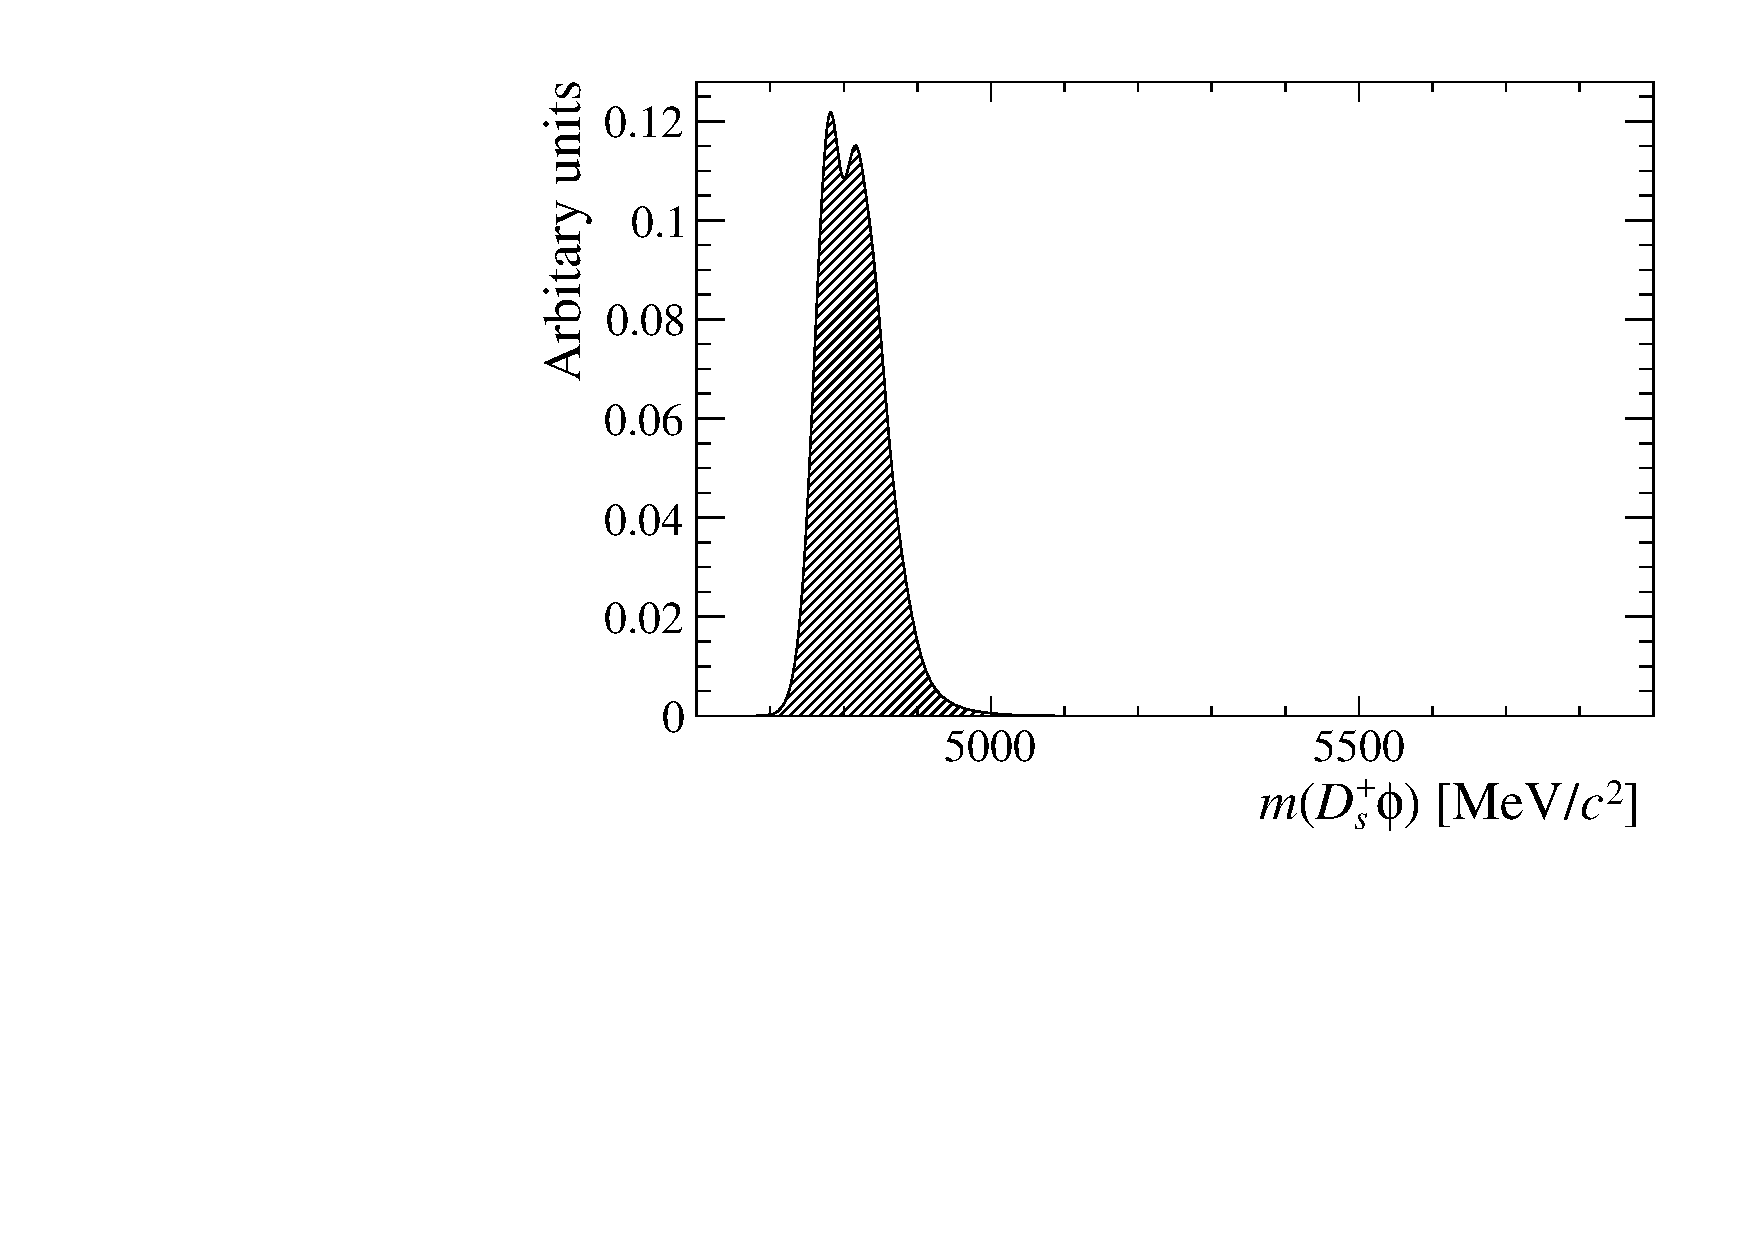
\includegraphics[width=1.0\textwidth]{figs/B2DsPhi/Bs2DsstDs_4600_5900_Shape.pdf}
        \caption{\decay{\Bsb}{\Dssp\Dsm} }
    \end{subfigure}
    \caption{Partially reconstructed mass PDFs determined from samples of simulations decays processed with the same reconstruction and selection as the signal decays. The \Bp meson mass is indicated by a vertical red line. The are below 4900\mevcc is not included in the fit range, but included for reference. The PDF colours follow the same convention used in the final fit plots shown in Fig.~\ref{fig:B2DsPhi_Signal_Fit}.}
    \label{fig:B2DsPhi_part_reco_shapes}   
\end{figure}
%%%%%%%%%%%%%%%%%%%%%%%%%%%%%%%%%%%%%%%%%%%%%%%%%%%%%%%%%%



% \begin{description}
% \item \textbf{\decay{\Bsb}{\Dsp\Km\Kstarz}:} this decay can form a background to \decay{\Bp}{\Dsp\phiz} decays when the soft pion from the \decay{\Kstarz}{\Kp\pim} decay is not reconstructed. The lower bound of the fit range is wide enough that a significant fraction of these decays are retained in the fitted data set. The $\Km\Kstarz$ is modelled as originating from the $a_1(1260)$ resonance. This resonance has a width of 250--600\mev~\cite{PDG2016}, allowing it to decay to $\Km\Kstarz$ even though it's pole mass is below the $\Km\Kstarz$ threshold. A PDF for this component is determined by reconstructing simulated \decay{\Bsb}{\Dsp\Km\Kstarz} decays through the identical reconstruction and selection steps as the signal. The \roofit class \texttt{RooKeysPDF} is used to create a kernel estimation of the partially reconstructed \Bp mass distribution for the candidates passing the selection. This is shown in Fig.~\ref{fig:B2DsPhi_part_reco_shapes_DsKKstar}. The fraction of these decays expected in each of the four $m(\Kp\Km)$ and $\cos\theta_{K}$ categories is determined from the simulations samples.
% \end{description}

% %%%%%%%%%%%%%%%%%%%%%%%%%%%%%%%%%%%%%%%%%%%%%%%%%%%%%%%%%%
% \begin{figure}[!h]
%     \centering
%     \begin{subfigure}[t]{0.49\textwidth}
%         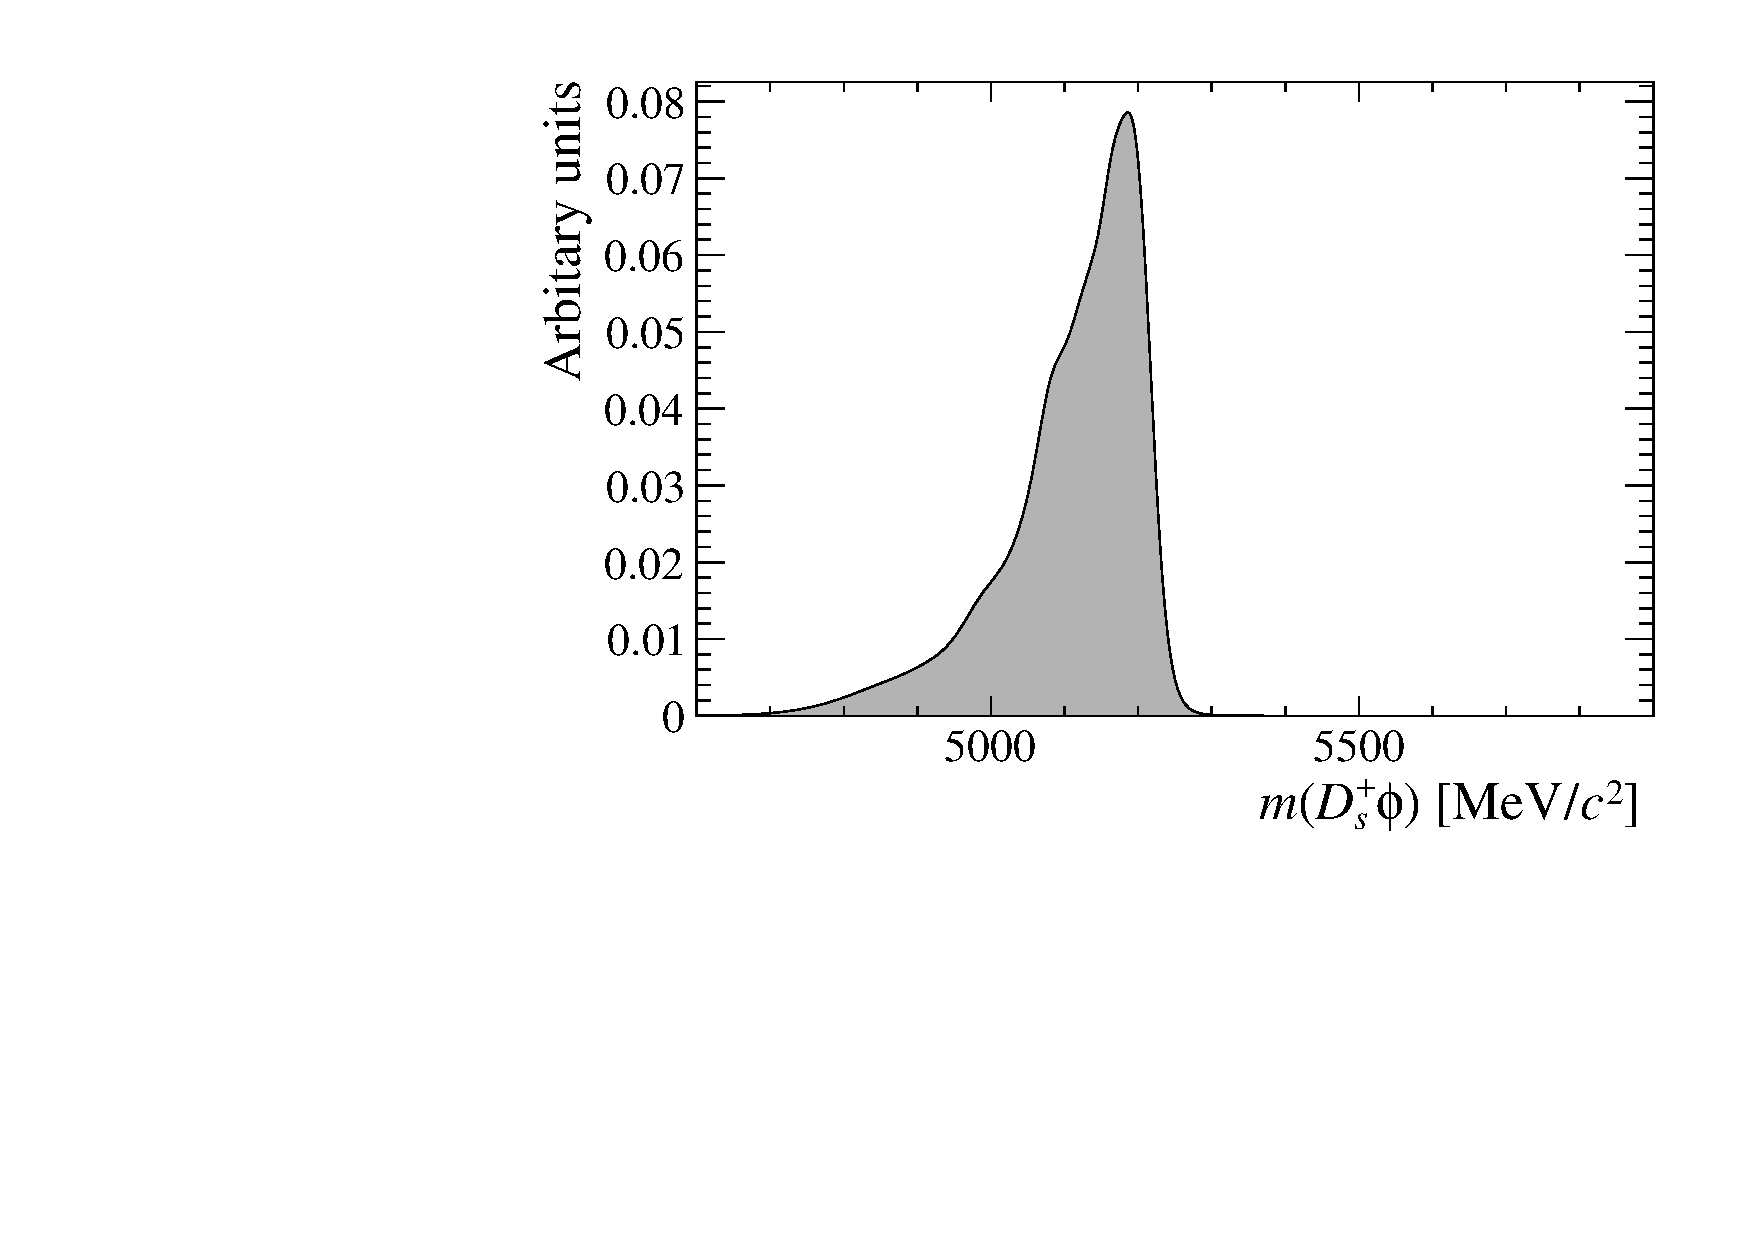
\includegraphics[width=1.0\textwidth]{figs/B2DsPhi/Bs2Dsa1_4600_5900_Shape.pdf}
%     \end{subfigure}
%     \caption{Partially reconstructed mass PDFs determined from samples of \decay{\Bsb}{\Dsp\Km\Kstarz} simulations processed with the same reconstruction and selection as the signal decays. The \Bp meson mass is indicated by a vertical red line. The are below 4900\mevcc is not included in the fit range, but included for reference. The PDF colours follow the same convention used in the final fit plots shown in Fig.~\ref{fig:B2DsPhi_Signal_Fit}.}
%     \label{fig:B2DsPhi_part_reco_shapes_DsKKstar}   
% \end{figure}
% %%%%%%%%%%%%%%%%%%%%%%%%%%%%%%%%%%%%%%%%%%%%%%%%%%%%%%%%%%

% \begin{description}
% \item \textbf{\decay{\Bsb}{\Dssp\Km\Kstarz}:} this decay similarly forms a background to the signal mode when both a low momentum neutral particle (\piz or \Pgamma) is not reconstructed in the decay of the \Dssp meson, in addition to the low momentum pion from the \Kstarz decay. The PDF is similarly determined using a kernel estimation from simulated decays passing the full selection as shown in Fig.~\ref{fig:B2DsPhi_part_reco_shapes_DsKKstar}. The fraction of candidates expected in each of the $m(\Kp\Km)$ and $\cos{\theta_{K}}$ categories are determined from these simulation samples.  

% \end{description}

% %%%%%%%%%%%%%%%%%%%%%%%%%%%%%%%%%%%%%%%%%%%%%%%%%%%%%%%%%%
% \begin{figure}[!h]
%     \centering
%     \begin{subfigure}[t]{0.49\textwidth}
%         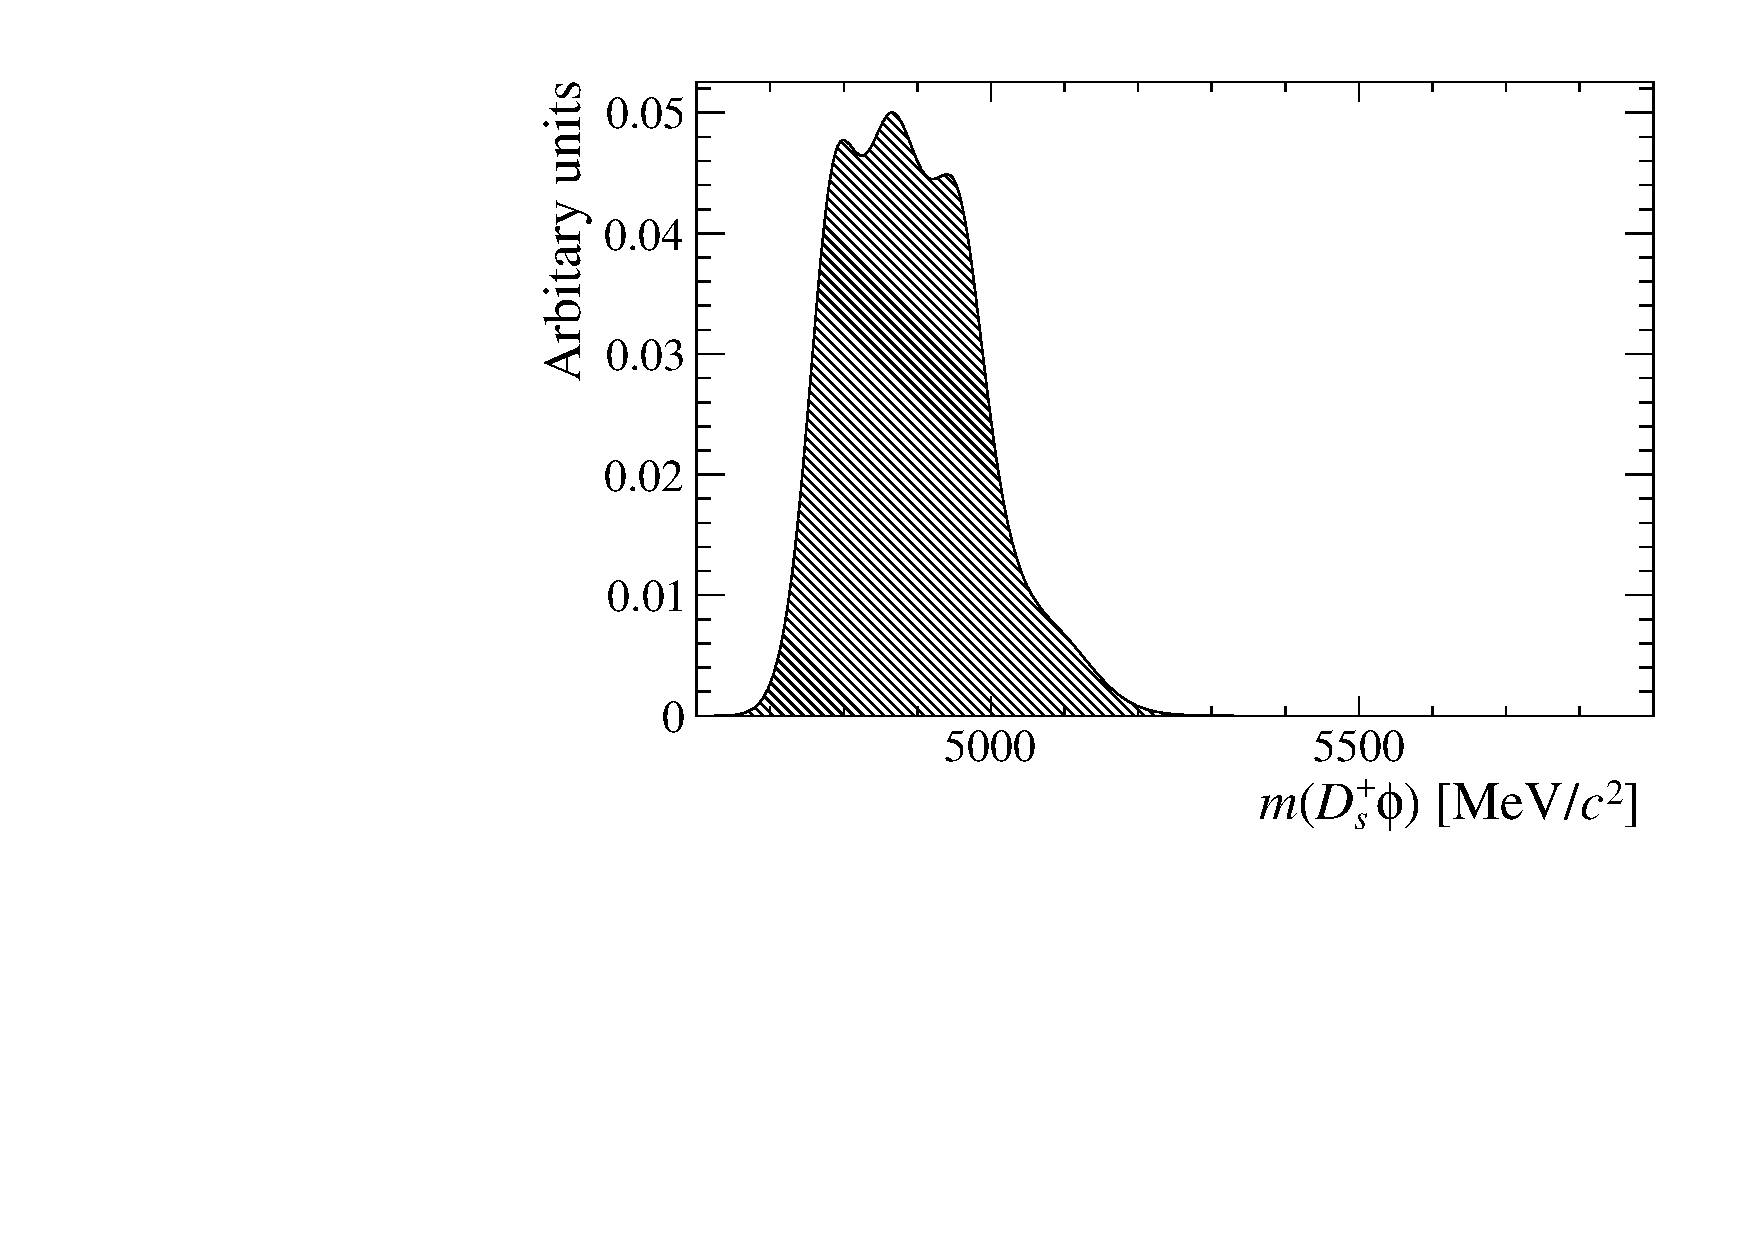
\includegraphics[width=1.0\textwidth]{figs/B2DsPhi/Bs2DsstKKst_4600_5900_Shape.pdf}
%     \end{subfigure}
%     \caption{Partially reconstructed mass PDFs determined from samples of \decay{\Bsb}{\Dssp\Km\Kstarz} simulations processed with the same reconstruction and selection as the signal decays. The \Bp meson mass is indicated by a vertical red line. The are below 4900\mevcc is not included in the fit range, but included for reference. The PDF colours follow the same convention used in the final fit plots shown in Fig.~\ref{fig:B2DsPhi_Signal_Fit}.}
%     \label{fig:B2DsPhi_part_reco_shapes_DsKKstar}   
% \end{figure}
% %%%%%%%%%%%%%%%%%%%%%%%%%%%%%%%%%%%%%%%%%%%%%%%%%%%%%%%%%%

% \begin{description}
% \item \textbf{\decay{\Bsb}{\Dsp\Dsm}, \decay{\Bzb}{\Dsp\Dm} and \decay{\Bsb}{\Dssp\Dsm}:} the decays of neutral \B mesons to two charged \D mesons can form a background to the signal decay if a low momentum pion is not reconstructed in one of the charm meson decays. In the case of \decay{\Bsb}{\Dssp\Dsm} decays an additional neutral particle is not reconstructed in the decay of the \Dssp meson.
% The PDFs for these decays are determined from simulated decays that have been processed with the same reconstruction and selection steps as the signal. For \decay{\Bsb}{\Dsp\Dsm} and \decay{\Bsb}{\Dssp\Dsm} decays, the PDF is creating using a kernel estimation using the \roofit \texttt{RooKeysPDF} implementation, shown in Fig.~\ref{fig:B2DsPhi_part_reco_shapes_DsDs}. Due to the similarities between \decay{\Bsb}{\Dsp\Dsm} and \decay{\Bzb}{\Dsp\Dm} decays, the PDF for the latter is created by using the kernel estimation for \decay{\Bsb}{\Dsp\Dsm} and shifting the shape down in mass by 40\mevcc to account for the kinematic differences. 

% The branching fractions for these three decays are measured to be $\BF(\decay{\Bzb}{\Dsp\Dm}) = (7.2 \pm 0.8 ) \times 10^{-3}$, $\BF(\decay{\Bsb}{\Dsp\Dsm}) = (4.4 \pm 0.5 ) \times 10^{-3}$ and $\BF(\decay{\Bsb}{\Dssp\Dsm}) = (1.37 \pm 0.16 ) \%$. Therefore the relative contributions for these three processes are fixed using these branching fractions, estimates of the relative efficiencies for each mode and the production fraction of \Bsb mesons relative to \Bzb mesons, $f_{s}/f_{d}$. This helps to add stability to the fit.   
% \end{description}


% %%%%%%%%%%%%%%%%%%%%%%%%%%%%%%%%%%%%%%%%%%%%%%%%%%%%%%%%%%
% \begin{figure}[!h]
%     \centering
%     \begin{subfigure}[t]{0.49\textwidth}
%         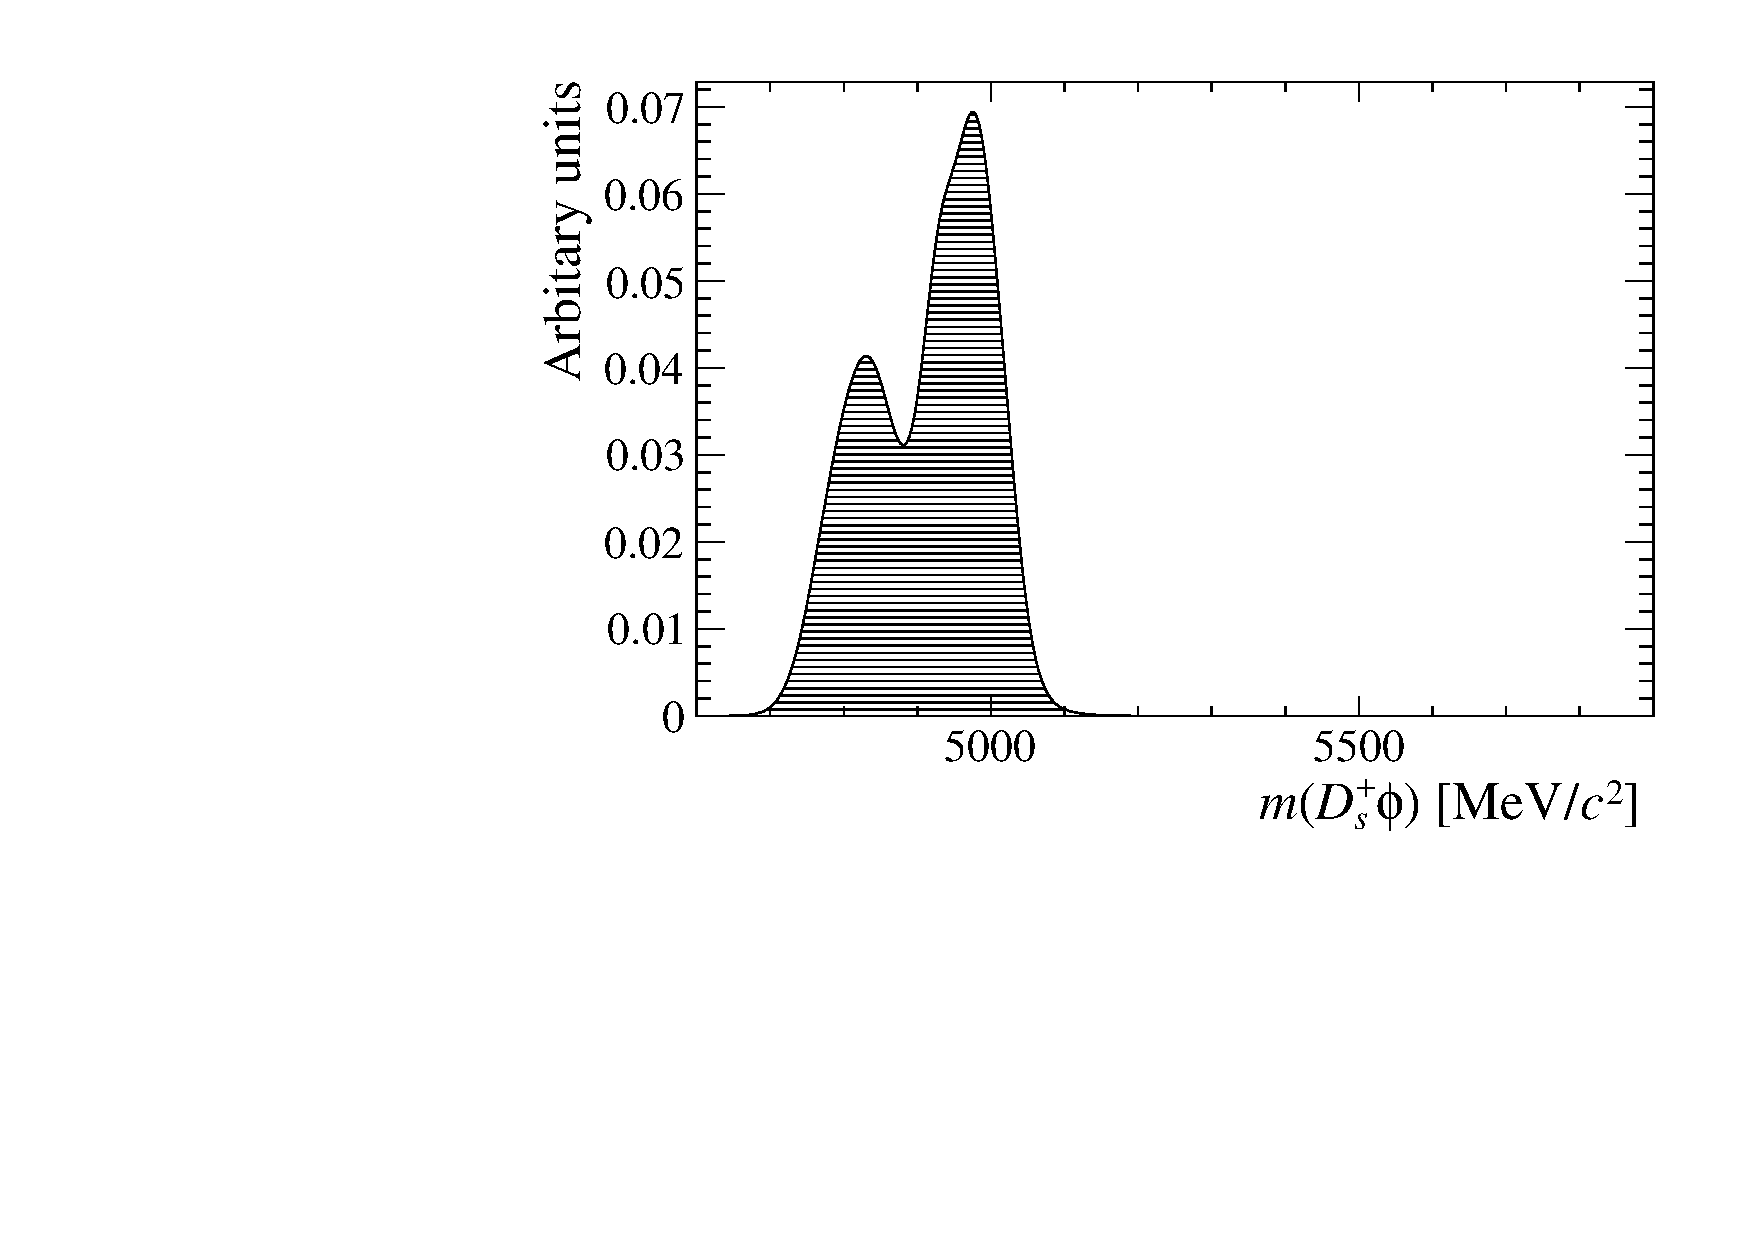
\includegraphics[width=1.0\textwidth]{figs/B2DsPhi/Bs2DsDs_4600_5900_Shape.pdf}
%         \caption{\decay{\Bsb}{\Dsp\Dsm} }
%     \end{subfigure}
%     \begin{subfigure}[t]{0.49\textwidth}
%         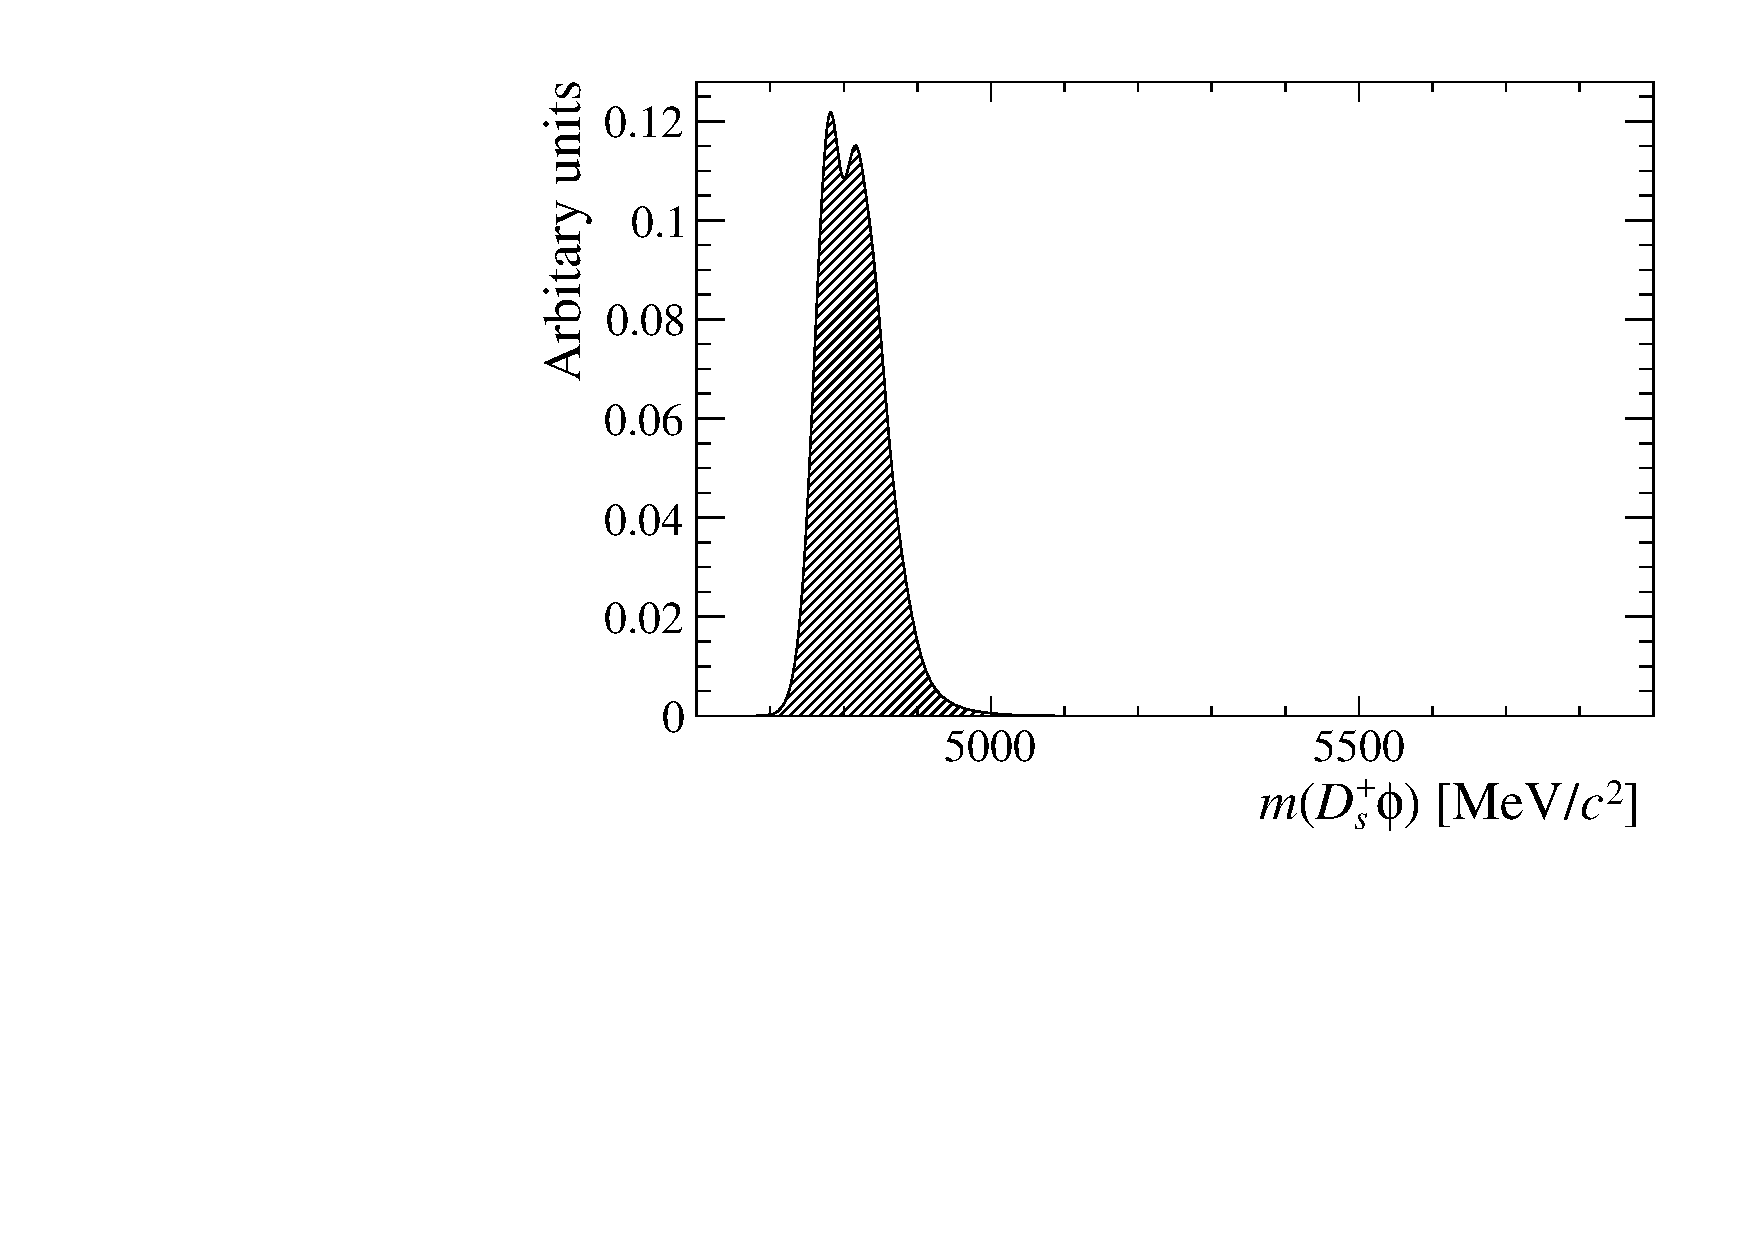
\includegraphics[width=1.0\textwidth]{figs/B2DsPhi/Bs2DsstDs_4600_5900_Shape.pdf}
%         \caption{\decay{\Bsb}{\Dssp\Dsm} }
%     \end{subfigure}
%     \caption{Partially reconstructed mass PDFs determined from samples of \decay{\Bsb}{\Dsp\Dsm} and \decay{\Bsb}{\Dssp\Dsm} simulations processed with the same reconstruction and selection as the signal decays. The \Bp meson mass is indicated by a vertical red line. The are below 4900\mevcc is not included in the fit range, but included for reference. The PDF colours follow the same convention used in the final fit plots shown in Fig.~\ref{fig:B2DsPhi_Signal_Fit}.}
%     \label{fig:B2DsPhi_part_reco_shapes_DsDs}   
% \end{figure}
% %%%%%%%%%%%%%%%%%%%%%%%%%%%%%%%%%%%%%%%%%%%%%%%%%%%%%%%%%%









\begin{description}
\item \textbf{\decay{\Bp}{(\decay{\Dssp}{\Dsp[\Pgamma]})\phiz} and \decay{\Bp}{(\decay{\Dssp}{\Dsp[\piz]})\phiz}:} the decays of \Bp mesons to an excited \Dsp meson and a \phiz meson could contribute to the $m(\Dsp\phiz)$ spectrum at low invariant masses when either a \piz or \Pgamma is missed from the excited meson decay. The resulting invariant mass distribution depends on the mass and spin of the non-reconstructed particle, as well as the helicity state of the \Dssp meson. This background involves the decay of a pseudo-scalar meson to two vector mesons, hence, as a result of angular momentum conservation, there are three helicity states of the \Dssp meson to consider. These are labelled \emph{001}, \emph{010} and \emph{100}. The two transversely polarised states, \emph{100} and \emph{001}, have identical invariant mass distributions and are therefore referred collectively as \emph{101}. This leads to a total of four contributions to consider for \decay{\Bp}{\Dssp\phiz} decays. These can be parametrised by parabolas convolved with resolution Gaussians in a similar way to the partially reconstructed backgrounds to the normalisation channel.
These each share the same functional form
\begin{equation}
f(m|a,b,\sigma,\xi, \delta) = \int_{a}^{b} g(\mu,a,b) \left( \frac{1-\xi}{b-a}\mu + \frac{b\xi-a}{b-a} \right) e^{-\frac{-(\mu-(m-\delta))^{2}}{2\sigma^{2}}} d\mu.
\label{eq:DsPhi_DsstarPhi_shapes}
\end{equation}
where $g(\mu,a,b)$ represents the parabola for each of the four components, listed in Table~\ref{tab:DsPhi_DsstarPhi_parabolas}. The resulting invariant mass distributions are shown in Fig.~\ref{eq:DsPhi_DsstarPhi_shapes}.

This decay is unobserved, therefore the relative contribution to this decay in nature from the \emph{101} and \emph{010} helicty states is not known. The total PDF for this contribution is made by weighting the \piz and \Pgamma contributions by their corresponding branching fractions, and by assuming that the \emph{101} and \emph{010} helicty states contribute with equal magnitudes. This assumption is varied and included as a source of systematic uncertainty in the $\BF(\decay{\Bp}{\Dsp\phiz})$ determination.
\end{description}
 
%%%%%%%%%%%%%%%%%%%%%%%%%%%%%%%%%%%%%%%%%%%%%%%%%%%%%%%%%% 
\begin{table}[h]
   \centering
   \begin{tabular}{ c c c c c }
      \hline
      Missed particle   & Helicity  & $g(\mu,a,b)$                                      & $a$ (\mevcc) & $b$ (\mevcc)  \\
      \hline
      \piz              & 010       & $\left(\mu - \frac{a+b}{2}\right)^{2}$            & 5026.8       & 5124.8         \\
      \piz              & 101       & $-(\mu - a)(\mu-b)$                               & 5026.8       & 5124.8         \\
      \Pgamma           & 010       & $-(\mu - a)(\mu-b)$                               & 4936.4       & 5220.6         \\
      \Pgamma           & 101       & $(\mu - \frac{a+b}{2})^{2} +(\frac{a+b}{2})^{2} $ & 4936.4       & 5220.6         \\
      \hline
   \end{tabular}
   \caption{The parabolas contributing to the partially reconstructed \decay{\Bp}{\Dssp\phiz} decay parametrisation as defined in Eq.~\ref{eq:DsPhi_DsstarPhi_shapes}. } 
   \label{tab:DsPhi_DsstarPhi_parabolas}  
\end{table}
%%%%%%%%%%%%%%%%%%%%%%%%%%%%%%%%%%%%%%%%%%%%%%%%%%%%%%%%%% 


%%%%%%%%%%%%%%%%%%%%%%%%%%%%%%%%%%%%%%%%%%%%%%%%%%%%%%%%%%
\begin{figure}[!h]
    \centering
    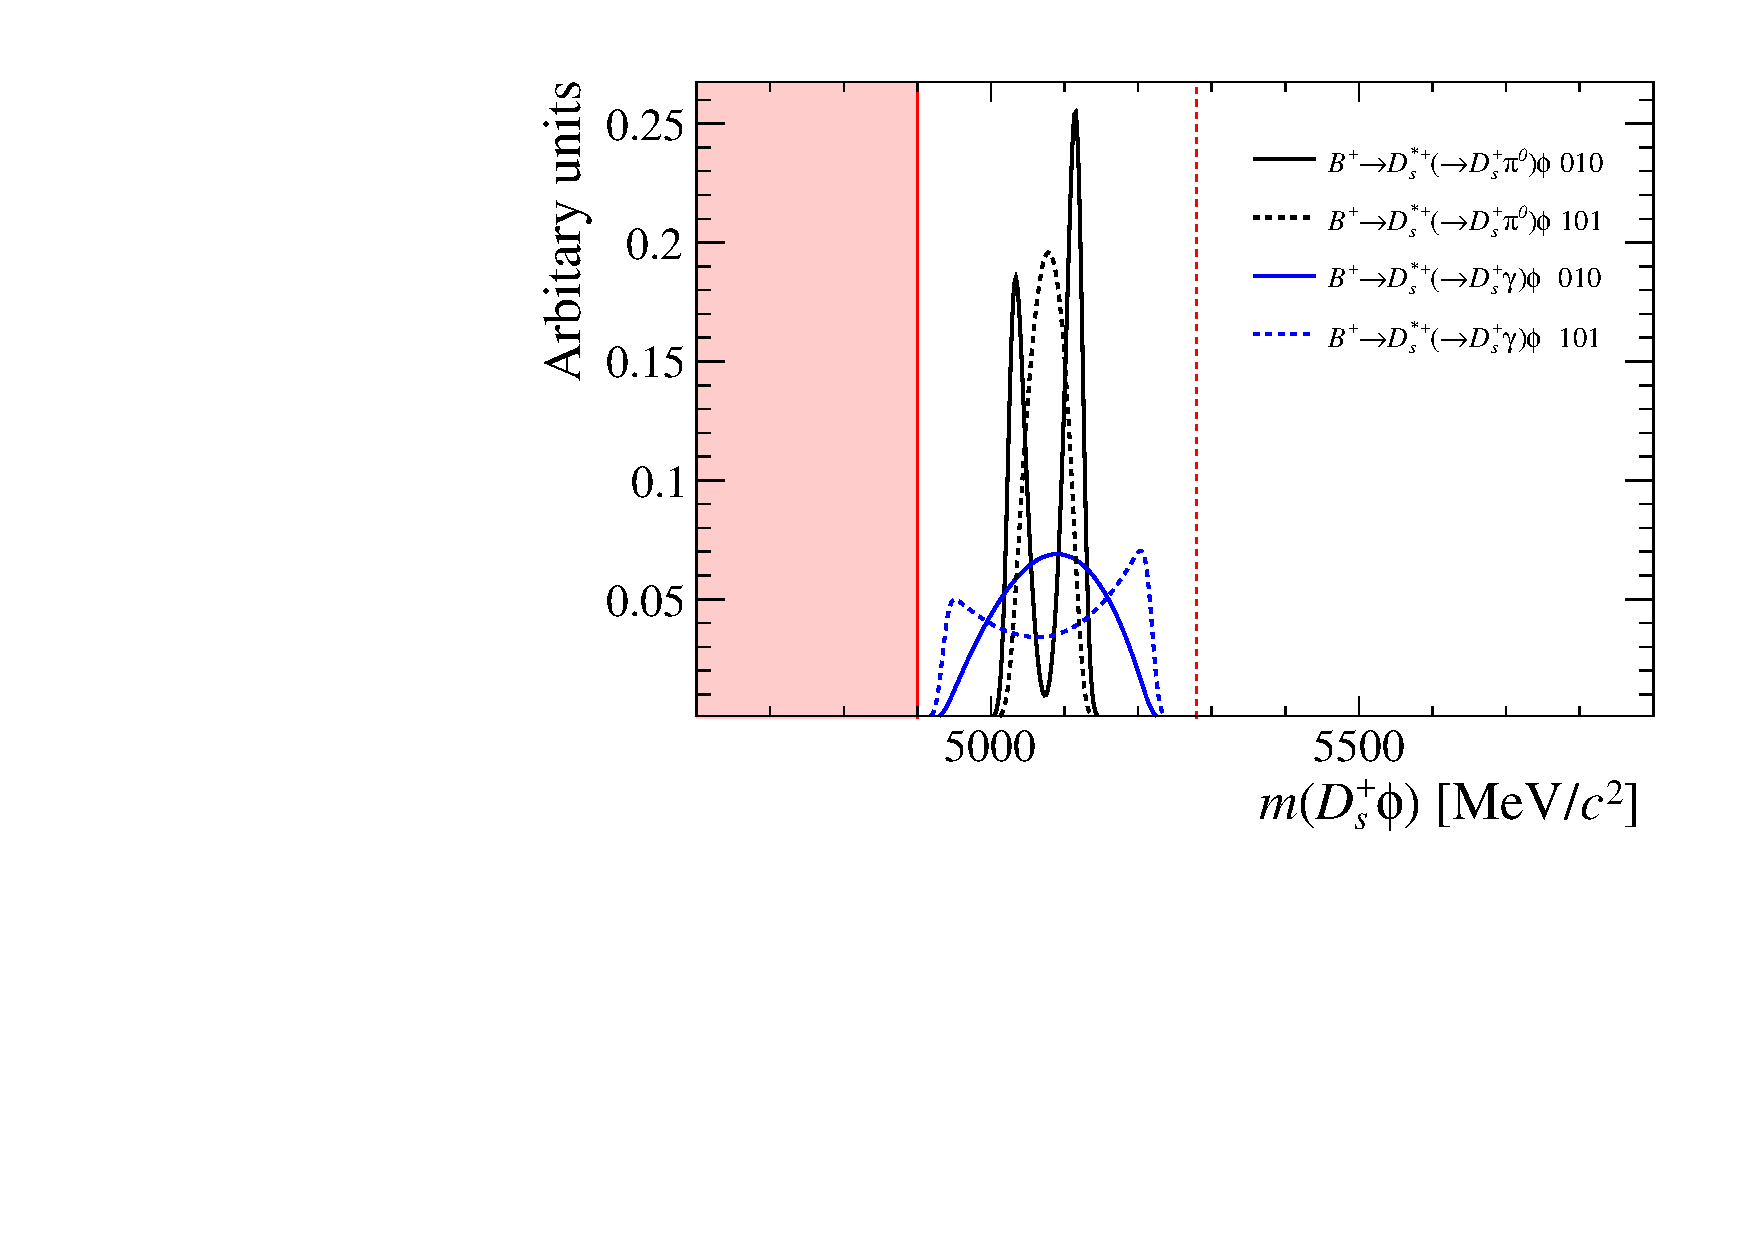
\includegraphics[width=0.70\textwidth]{figs/B2DsPhi/DsPhi_part_reco_Shapes.pdf}
    \caption{Partially reconstructed \decay{\Bp}{\Dssp\phiz} PDFs as described in Sec.~\ref{sec:B2DsPhi_part_recto_sig}. The range below $4900\mevcc$ (highlighted in red) is not included in the fit range, but included to shown the full PDF distributions. The \Bp meson mass is represented by a dashed vertical line.}
    \label{fig:B2DsPhi_DsPhi_partreco}   
\end{figure}
%%%%%%%%%%%%%%%%%%%%%%%%%%%%%%%%%%%%%%%%%%%%%%%%%%%%%%%%%%


% {\color{Blue}
% Additionally, the distribution of each shape in the helicity angle described in Section~\ref{subsec:Hel} is approximated to be $\cos^2(\theta)$ for the longitudinally polarized shapes (010) and $\sin^2(\theta)$ for the transversely (101). The fraction in each bin for 010 or 101 is taken from the appropriate integrals of these assumed distributions. 
% }



To account for difference between the simulation and data samples all PDFs determined using the kernel estimation method are convolved with an additional Gaussian. The mean position of this Gaussian is given by $\delta$, the same offset used for the analytically described partially decays. The width of the Gaussian is increased to account for the difference in resolution between simulation and data. 


\subsection{Combinatorial  backgrounds}
\label{sec:B2DsPhi_combcomps}

Combinations of unrelated tracks form a background to the signal decays and extend across the entire fitted \Bp meson mass range. 
This component is parametrised with a decaying exponential function 
\begin{equation}
f(m|c) = e^{-mc},
\end{equation}
where the parameter $c$ controls the slope and $m$ is the observable \Bp meson invariant mass. 
The combinatorial background is the dominant background under the signal decays, therefore it is important to accurately extrapolate distribution from the high and low mass ranges to the signal range. 

The yields of combinatorial background is allowed to vary freely in each of the separate simultaneous fit categories. To improve the stability of the fit, the single slope parameter, $c$, is shared between all of the categories. 
%In categories with lower statistics, for example the \decay{\Dsp}{\Kp\pim\pip} decay mode, it would be possible for the partially reconstructed backgrounds to be incorrectly assigned to the combinatorial component. This can happen if the exponential slope for that mode gets to large, causing it to `kick up' at low invariant masses. This may bias the signal yield in this mode. Fixing the slope parameter to be the same between the different \Dsp modes and between the signal and normalisation channel allows the lower statistics modes to benefit from those with higher statistics.

\section{Free and constrained parameters}

The fit to \decay{\Bp}{\Dsp\phiz} and \decay{\Bp}{\Dsp\Dzb} decays contains a total of 54 free parameters. 
These are divided into four different categories;

%These are listed in Tab.~\ref{tab:B2DsPhi_free_variables}. 

\subsection{Parameter of interest}

The parameter of interest (POI) is the branching fraction for \decay{\Bp}{\Dsp\phiz} decays. This is determined directly in the fit to the signal and normalisation decays. The same single branching fraction is used for all of the \Dsp decays modes.
The yield of signal candidates is calculated using the equation 
\begin{equation}
N(\decay{\Bp}{\Dsp\phiz}) = k_{\Dsp} \times \BF(\decay{\Bp}{\Dsp\phiz}) \times N(\decay{\Bp}{\Dsp\Dzb}),
\end{equation}
where $k_{\Dsp}$ is a constant defined for each \Dsp decay mode
\begin{equation}
k_{\Dsp} = \frac{\epsilon(\decay{\Bp}{\Dsp\Dzb})}{\epsilon(\decay{\Bp}{\Dsp\phiz})} \times  \frac{\BF(\decay{\phiz}{\Kp\Km})}{\BF(\decay{\Bp}{\Dsp\Dzb})\BF(\decay{\Dzb}{\Kp\Km})}.
\end{equation}
Here, the efficiencies $\epsilon$ are calculated for the specific \Dsp decay mode in question and external measurements are used for the additional branching fractions.
The yield $N(\decay{\Bp}{\Dsp\phiz})$ is the total signal yield in all four $m(\Kp\Km)$ and $\cos\theta_{K}$ categories. The yields in each category are constrained to be in the ratios previously listed in Table~\ref{tab:signal_ratios}, \ie the yield in the $|m(\Kp\Km)<10\mevcc$ and $|\cos\theta_{K}|>0.4$ category is $0.82\times N(\decay{\Bp}{\Dsp\phiz})$.



\subsection{Shape parameters}
As detailed in Sec~\ref{sec:B2DsPhi_fitcomponents}, the fit included eight parameters governing the shapes of various PDFs.
\begin{itemize}
\item The combinatorial background PDF is controlled by a single slope parameter $c$ for all categories.
\item The mean \Bp mass for the signal and normalisation mode is free to vary in the fit. The same value is used for all \decay{\Bp}{\Dsp\phiz} and \decay{\Bp}{\Dsp\Dzb} PDFs.
\item The invariant mass offset $\delta$ shared between all partially reconstructed background PDFs is allowed to freely vary in the fit. The same value is used for the signal and normalisation modes.
\item The relative heights of the two peaks in partially reconstructed \decay{\Bp}{\Dssp\phiz}, \decay{\Bp}{\Dssp\Dzb} and \decay{\Bp}{\Dsp\Dstarzb} decays, $\xi$, is allowed to vary. The same value is used for all modes.
\item The smaller CB width parameter, $\sigma_{1}$, is allowed to vary for each of the \Dsp decay modes, leading to four more free parameters. 
\end{itemize}

\subsection{Yields}

The fit model contains a total of 36 free parameters that are yields.
\begin{itemize}
\item The total yield of normalisation decays in each \Dsp decay mode is left floating in the fit. These variables are the sum of the yields in the two helicity categories, $|\cos\theta_{K}| < 0.4$ and $|\cos\theta_{K}| > 0.4$. This results in four free parameters.
\item The yield of certain partially reconstructed decays in the normalisation channel is left floating for each \Dsp decay mode independently. This yield is defined to be $N(\decay{\Bp}{\Dsp\Dstarzb})+ N(\decay{\Bp}{\Dssp\Dzb})$. The yield of the doubly excited \decay{\Bp}{\Dssp\Dstarzb} is not included in this total. This results in four free parameters.
\item The yield of some partially reconstructed decays in the signal mode is left free in the fit. This is defined to be $N(\Dssp\phiz) + N(\Dsp\Km\Kstarz) + N(\Dssp\Km\Kstarz)$. This leads to four free parameters. 
\item All yields of combinatorial backgrounds are left free in the fit. This results in 24 free parameters.
\end{itemize}



\subsection{Fractions}




The majority of the partially reconstructed backgrounds do not have unconstrained yields in each of the 24 simultaneous fit categories. 
Instead, a single partially reconstructed background yield per \Dsp decay mode is left free in the fit. The relative contributions of other partially backgrounds are determined by floating fraction parameters multiplied by this yield. 
This allows the different background contributions to vary relative to one another, but keeps the ratios of the relative contributions the same across the different \Dsp decay modes.

There are four free parameters controlling the backgrounds contributions in the signal mode:
\begin{enumerate}
\item Ratio of yields of \decay{\Bp}{\Dsp\Kp\Km} decays to \decay{\Bp}{\Dsp\Dzb} decays
\begin{equation}
\frac{N(\decay{\Bp}{\Dsp\Kp\Km})}{N(\decay{\Bp}{\Dsp\Dzb})}. 
\end{equation}
\item The fraction of \decay{\Bsb}{\Dsp\Km\Kstarz} decays to the total of $\decay{\Bsb}{D_{s}^{(*)+}\Km\Kstarz}$ decays
\begin{equation}
\frac{N(\decay{\Bsb}{\Dsp\Km\Kstarz})}{N(\decay{\Bsb}{\Dssp\Km\Kstarz})+N(\decay{\Bsb}{\Dsp\Km\Kstarz})}.
\end{equation}

\item The fraction of \decay{\Bp}{\Dssp\phiz} decays in the total of these and $\decay{\Bsb}{D_{s}^{(*)+}\Km\Kstarz}$ decays
\begin{equation}
\frac{N(\decay{\Bp}{\Dssp\phiz})}{N(\decay{\Bp}{\Dssp\phiz})+N(\decay{\Bsb}{\Dssp\Km\Kstarz})+N(\decay{\Bsb}{\Dsp\Km\Kstarz})}   
\end{equation}
\item The ratio of yields of the partially reconstructed \decay{\Bs}{\Dsp\Dsm}, \decay{\Bs}{\Dsp\Dssm} and \decay{\Bz}{\Dsp\Dm} decays to $\decay{\Bp}{\Dssp\phiz}$ and $\decay{\Bsb}{D_{s}^{(*)+}\Km\Kstarz}$ decays
\begin{equation}
\frac{N(\decay{\Bs}{\Dsp\Dsm})+ N(\decay{\Bs}{\Dsp\Dssm}) + N(\decay{\Bz}{\Dsp\Dm})}{N(\decay{\Bp}{\Dssp\phiz})+N(\decay{\Bsb}{\Dssp\Km\Kstarz})+N(\decay{\Bsb}{\Dsp\Km\Kstarz})}   
\end{equation}


\end{enumerate}


Another five free parameters control the fractions of events in different categories for the normalisation mode:

\begin{enumerate}
\item Fraction of partially reconstructed \decay{\Bp}{\Dssp\Dzb} decays in the total of \decay{\Bp}{\Dssp\Dzb} and \decay{\Bp}{\Dsp\Dstarzb} decays in the $|\cos\theta_{K}|>0.4$ category
\begin{equation}
\left(\frac{N(\decay{\Bp}{\Dssp\Dzb})}{N(\decay{\Bp}{\Dssp\Dzb})+N(\decay{\Bp}{\Dsp\Dstarzb})}\right)_{|\cos\theta_{K}|>0.4}   
\end{equation}
\item Fraction of partially reconstructed \decay{\Bp}{\Dssp\Dzb} decays in the total of \decay{\Bp}{\Dssp\Dzb} and \decay{\Bp}{\Dsp\Dstarzb} decays in the alternative $|\cos\theta_{K}|<0.4$ category
\begin{equation}
\left(\frac{N(\decay{\Bp}{\Dssp\Dzb})}{N(\decay{\Bp}{\Dssp\Dzb})+N(\decay{\Bp}{\Dsp\Dstarzb})}\right)_{|\cos\theta_{K}|<0.4}   
\end{equation}
\item Fraction of partially reconstructed backgrounds in the $|\cos\theta_{K}|>0.4$ category
\begin{equation}
\frac{(N(\decay{\Bp}{\Dssp\Dzb})+N(\decay{\Bp}{\Dsp\Dstarzb}))_{|\cos\theta_{K}|>0.4}}{(N(\decay{\Bp}{\Dssp\Dzb})+N(\decay{\Bp}{\Dsp\Dstarzb}))_{\text{Total}}}   
\end{equation}
\item The ratio of \decay{\Bp}{\Dssp\Dstarzb} decays to the total of \decay{\Bp}{\Dssp\Dzb} and \decay{\Bp}{\Dsp\Dstarzb} decays
\begin{equation}\frac{N(\decay{\Bp}{\Dssp\Dstarzb})}{N(\decay{\Bp}{\Dssp\Dzb})+N(\decay{\Bp}{\Dsp\Dstarzb})}   
\end{equation}
\item Fraction of fully reconstructed normalisation decays in the $|\cos\theta_{K}|>0.4$ category
\begin{equation}
\frac{N(\decay{\Bp}{\Dsp\Dzb})_{|\cos\theta_{K}|>0.4}}{N(\decay{\Bp}{\Dsp\Dzb})_{\text{Total}}}.   
\end{equation}
This parameter is included as a cross check. The normalisation decays have a flat distribution in $\cos\theta_{K}$ so the paremeter would be expected to be around $0.6$. 
\end{enumerate}



% \begin{longtable}{ l l }
% \hline
% Type & Variable  \\
% \hline
% POI                  & Branching fraction $\BF(\decay{\Bp}{\Dsp\phiz})$                              \\
% \hline 
% Shape                & Combinatorial slope $c$                                                           \\ 
%                      & Mean \Bp mass (\mevcc)                                                        \\  
%                      & Mass offset $\delta$ (\mevcc)                         \\  
%                      & Relative heights $\xi$                               \\
%                      & $\sigma_{1}$ for \decay{\Dsp}{\Kp\Km\pip}  (\mevcc)                           \\  
%                      & $\sigma_{1}$ for \decay{\Dsp}{\Kp\pim\pip} (\mevcc)                           \\  
%                      & $\sigma_{1}$ for \decay{\Dsp}{\phiz\pip}  (\mevcc)                            \\  
%                      & $\sigma_{1}$ for \decay{\Dsp}{\pip\pim\pip}  (\mevcc)                         \\  
% \hline  
% Yields               & $N(\decay{\Bp}{(\decay{\Dsp}{\Kp\Km\pip}  )\Dzb})$                 \\  
%                      & $N(\decay{\Bp}{(\decay{\Dsp}{\Kp\pim\pip} )\Dzb})$                 \\  
%                      & $N(\decay{\Bp}{(\decay{\Dsp}{\phiz\pip}   )\Dzb})$                 \\  
%                      & $N(\decay{\Bp}{(\decay{\Dsp}{\pip\pim\pip})\Dzb})$                 \\
%                      & $N(\Dssp\Dzb + \Dsp\Dstarzb)$ in \decay{\Dsp}{\Kp\Km\pip}               \\  
%                      & $N(\Dssp\Dzb + \Dsp\Dstarzb)$ in \decay{\Dsp}{\Kp\pim\pip}              \\  
%                      & $N(\Dssp\Dzb + \Dsp\Dstarzb)$ in \decay{\Dsp}{\phiz\pip}                \\  
%                      & $N(\Dssp\Dzb + \Dsp\Dstarzb)$ in \decay{\Dsp}{\pip\pim\pip}             \\  
%                      & $N(\Dssp\phiz + D_{s}^{(*)+}\Km\Kstarz)$ in \decay{\Dsp}{\Kp\Km\pip}       \\  
%                      & $N(\Dssp\phiz + D_{s}^{(*)+}\Km\Kstarz)$ in \decay{\Dsp}{\Kp\pim\pip}      \\  
%                      & $N(\Dssp\phiz + D_{s}^{(*)+}\Km\Kstarz)$ in \decay{\Dsp}{\phiz\pip}        \\  
%                      & $N(\Dssp\phiz + D_{s}^{(*)+}\Km\Kstarz)$ in \decay{\Dsp}{\Kp\pim\pip}      \\

%                      & $N_{\text{comb}}((\decay{\Dsp}{\Kp\Km\pip})\Dzb)$  in H1             \\  
%                      & $N_{\text{comb}}(\Dsp\Dzb)$ \decay{\Dsp}{\Kp\Km\pip} in H2             \\  
%                      & $N_{\text{comb}}(\Dsp\Dzb)$ \decay{\Dsp}{\Kp\pim\pip} in H1            \\  
%                      & $N_{\text{comb}}(\Dsp\Dzb)$ \decay{\Dsp}{\Kp\pim\pip} in H2            \\  
%                      & $N_{\text{comb}}(\Dsp\Dzb)$ \decay{\Dsp}{\phiz\pip} in H1              \\  
%                      & $N_{\text{comb}}(\Dsp\Dzb)$ \decay{\Dsp}{\phiz\pip} in H2              \\  
%                      & $N_{\text{comb}}(\Dsp\Dzb)$ \decay{\Dsp}{\pip\pim\pip} in H1           \\  
%                      & $N_{\text{comb}}(\Dsp\Dzb)$ \decay{\Dsp}{\pip\pim\pip} in H2           \\    
%                      & $N_{\text{comb}}(\Dsp\phiz)$ \decay{\Dsp}{\Kp\Km\pip} in H1            \\  
%                      & $N_{\text{comb}}(\Dsp\phiz)$ \decay{\Dsp}{\Kp\Km\pip} in H2            \\  
%                      & $N_{\text{comb}}(\Dsp\phiz)$ \decay{\Dsp}{\Kp\pim\pip} in H1           \\  
%                      & $N_{\text{comb}}(\Dsp\phiz)$ \decay{\Dsp}{\Kp\pim\pip} in H2           \\  
%                      & $N_{\text{comb}}(\Dsp\phiz)$ \decay{\Dsp}{\phiz\pip} in H1             \\  
%                      & $N_{\text{comb}}(\Dsp\phiz)$ \decay{\Dsp}{\phiz\pip} in H2             \\  
%                      & $N_{\text{comb}}(\Dsp\phiz)$ \decay{\Dsp}{\pip\pim\pip} in H1          \\  
%                      & $N_{\text{comb}}(\Dsp\phiz)$ \decay{\Dsp}{\pip\pim\pip} in H2          \\
%                      & $N_{\text{comb}}(\Dsp\phiz)$ \phiz-sideband \decay{\Dsp}{\Kp\Km\pip} in H1   \\  
%                      & $N_{\text{comb}}(\Dsp\phiz)$ \phiz-sideband \decay{\Dsp}{\Kp\Km\pip} in H2   \\  
%                      & $N_{\text{comb}}(\Dsp\phiz)$ \phiz-sideband \decay{\Dsp}{\Kp\pim\pip} in H1  \\  
%                      & $N_{\text{comb}}(\Dsp\phiz)$ \phiz-sideband \decay{\Dsp}{\Kp\pim\pip} in H2  \\  
%                      & $N_{\text{comb}}(\Dsp\phiz)$ \phiz-sideband \decay{\Dsp}{\phiz\pip} in H1    \\  
%                      & $N_{\text{comb}}(\Dsp\phiz)$ \phiz-sideband \decay{\Dsp}{\phiz\pip} in H2    \\  
%                      & $N_{\text{comb}}(\Dsp\phiz)$ \phiz-sideband \decay{\Dsp}{\pip\pim\pip} in H1 \\  
%                      & $N_{\text{comb}}(\Dsp\phiz)$ \phiz-sideband \decay{\Dsp}{\pip\pim\pip} in H2 \\ 
% \hline 
% Fractions            & Ratio of \Dsp\Kp\Km to \Dsp\Dzb                                        \\  
%                      & Fraction of \Dsp\Km\Kstarz in (\Dssp\Km\Kstarz+\Dsp\Km\Kstarz)                    \\ 
%                      & Fraction of $\Dssp\phiz$ in ($D_{s}^{(*)+}\Km\Kstarz$ + $\Dssp\phiz$)                   \\  
%                      & Ratio of $\Dsp D_{(s)}^{(*)-}$ to ($\Dssp\phiz$ + $D_{s}^{(*)+}\Km\Kstarz$)           \\  

%                      & Fraction of \Dssp\Dzb in (\Dssp\Dzb+\Dsp\Dstarzb) in H1         \\  
%                      & Fraction of \Dssp\Dzb in (\Dssp\Dzb+\Dsp\Dstarzb) in H2         \\ 
%                      & Fraction of normalisation part reco in H1                       \\  
%                      & Fraction of normalisation peak in H1                            \\ 
%                      & Ratio of \Dssp\Dstarzb to (\Dssp\Dzb + \Dsp\Dstarzb)                          \\ 
% \hline
% \caption{The fit result with final values of all floating variables used in the fit model. Here H1 and H2 represent the $|\cos\theta_{K}|>0.4$ and $|\cos\theta_{K}|<0.4$ categories respectively.} 
% \label{tab:B2DsPhi_free_variables} 
% \end{longtable}

\section{Fit validation}
\label{sec:B2DsPhi_fitstrategy}
The simultaneous fitting framework is validated by generating pseudo-experiments using a similar procedure as described in the search for \decay{\Bp}{\Dsp\Kp\Km} decays. The frame work is found to not have any significant bias as described in Appendix~\ref{ch:appendix_toys}.


% The simultaneous fitting framework is validated by generating pseudo-experiments (also referred to as \emph{toys}). The total fit model PDF is randomly sampled to create a simulation sample with the same number of candidates as the nominal fit. These are then fitted using the same fit model, determining the best estimate and uncertainty of each parameter. The parameter values used to generate the pseudo-experiments are chosen to be the final parameter values as determined in a fit to data. This is known as the plug-in method~\cite{plugin}.
% The fitted value and associated error is used to determine the pull of each parameter of interest. As the errors are determined asymmetrically using \minos the is defined conditionally to incorporate the appropriate error 
% \begin{equation}
%   g_{\text{pull}} = \left \{
%   \begin{aligned}
%     &\frac{x_{\text{gen}} - x_{\text{fit}} }{\sigma_{+}}, && \text{if}\ x_{\text{fit}} < x_{\text{gen}}\\
%     &\frac{x_{\text{fit}} - x_{\text{gen}} }{\sigma_{-}}, && \text{otherwise},
%   \end{aligned} \right.
% \end{equation} 
% where $x_{\text{fit}}$ and $x_{\text{gen}}$ are the fitted and generated values of the variable, and $\sigma_{+}$ and $\sigma_{-}$ are the high and low asymmetric errors.

% The distributions of the values, errors and pulls for the yields of the normalisation decay in each of the \Dsp decays are shown in Fig.~\ref{fig:B2DsPhi_Pulls_normalisation}. The mean and widths are determined using simple fits to the pull distributions. The results and PDFs for these fits are overlaid on the distributions. The normalisation yield means and widths are found to be within $2\sigma$ of zero and one respectively.


% %%%%%%%%%%%%%%%%%%%%%%%%%%%%%%%%%%%%%%%%%%%%%%%%%%%%%%%%%%
% \begin{figure}[!h]
%    \centering
%    \begin{subfigure}[t]{1.0\textwidth}
%       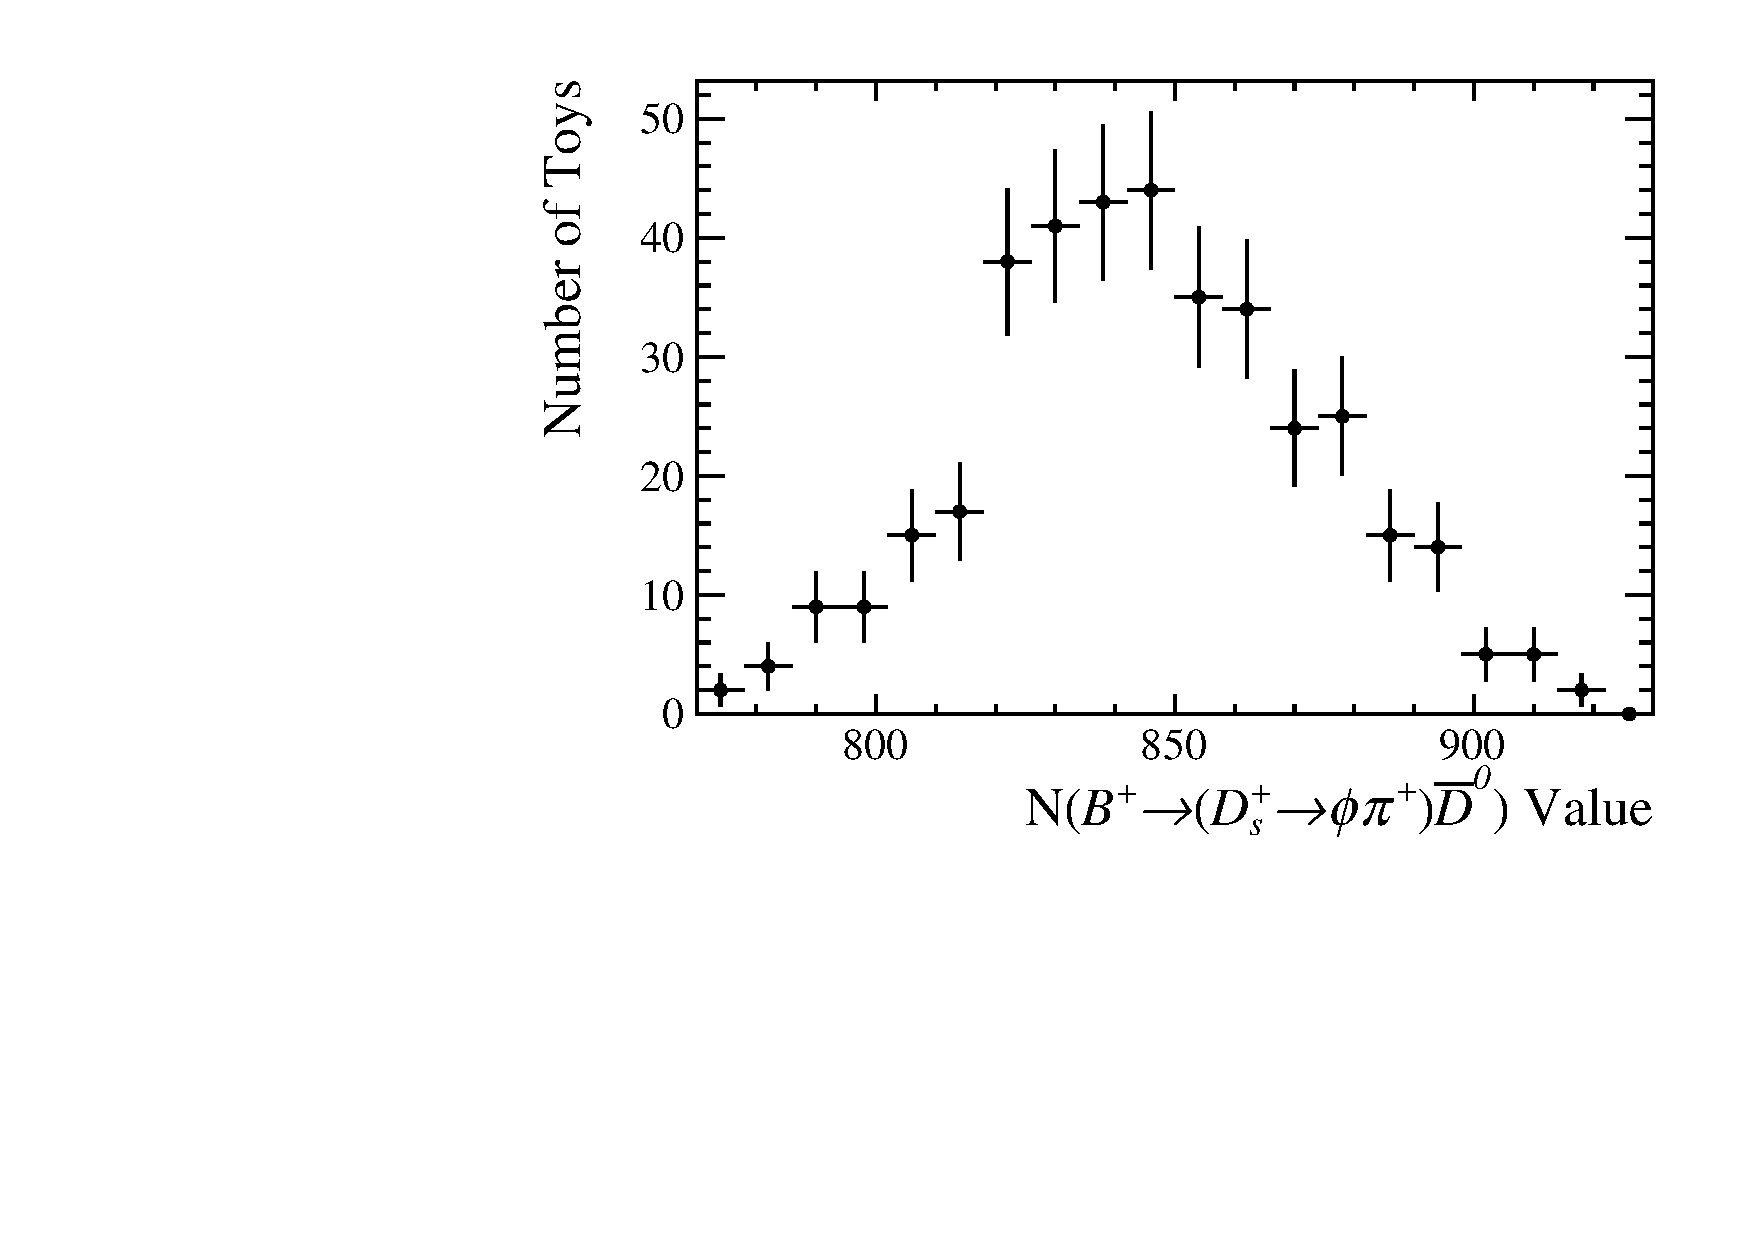
\includegraphics[width=0.32\textwidth]{figs/B2DsPhi/Plots_DsKK_Value_yield_peak_DsD0_Ds2PhiPi_toy_both_DsBDTbin1_PhiBDTbin1_both_both.pdf}
%       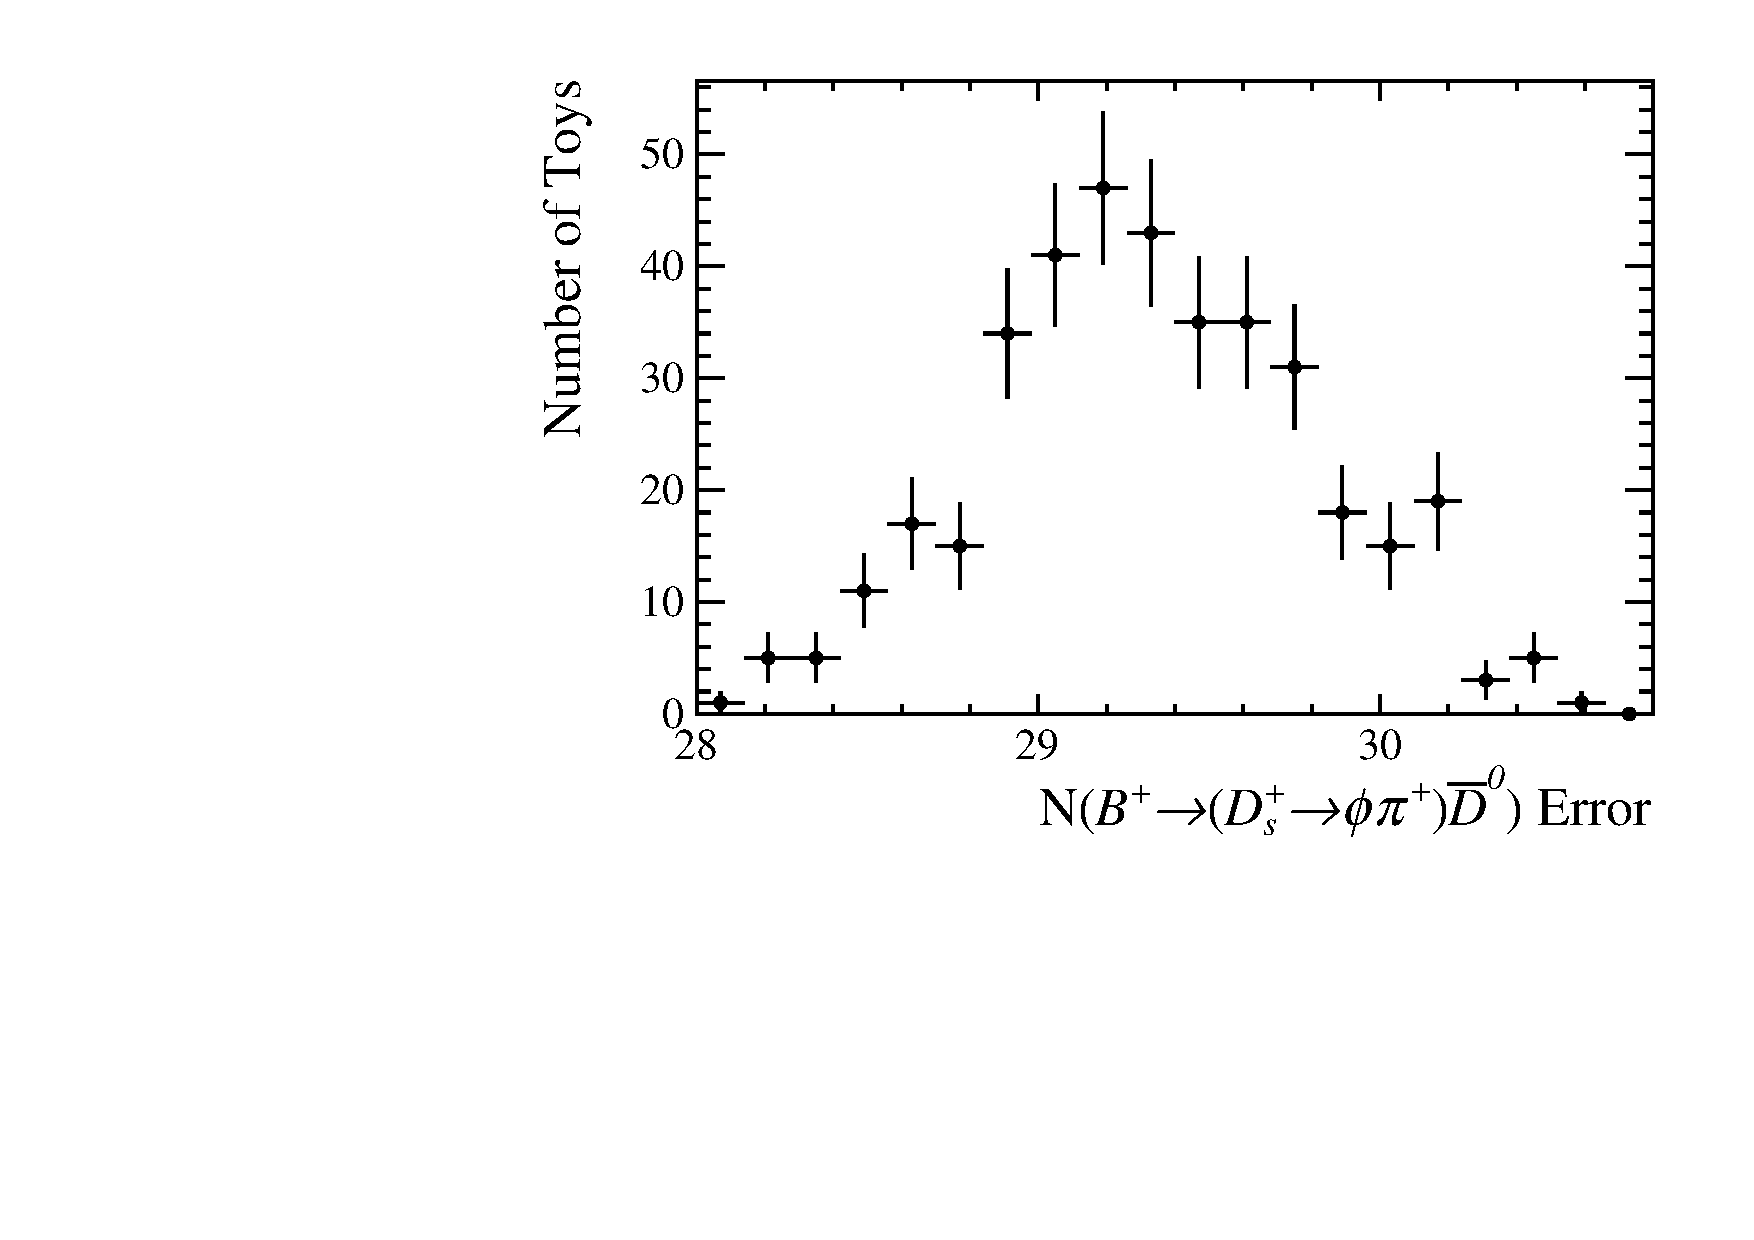
\includegraphics[width=0.32\textwidth]{figs/B2DsPhi/Plots_DsKK_Error_yield_peak_DsD0_Ds2PhiPi_toy_both_DsBDTbin1_PhiBDTbin1_both_both.pdf}
%       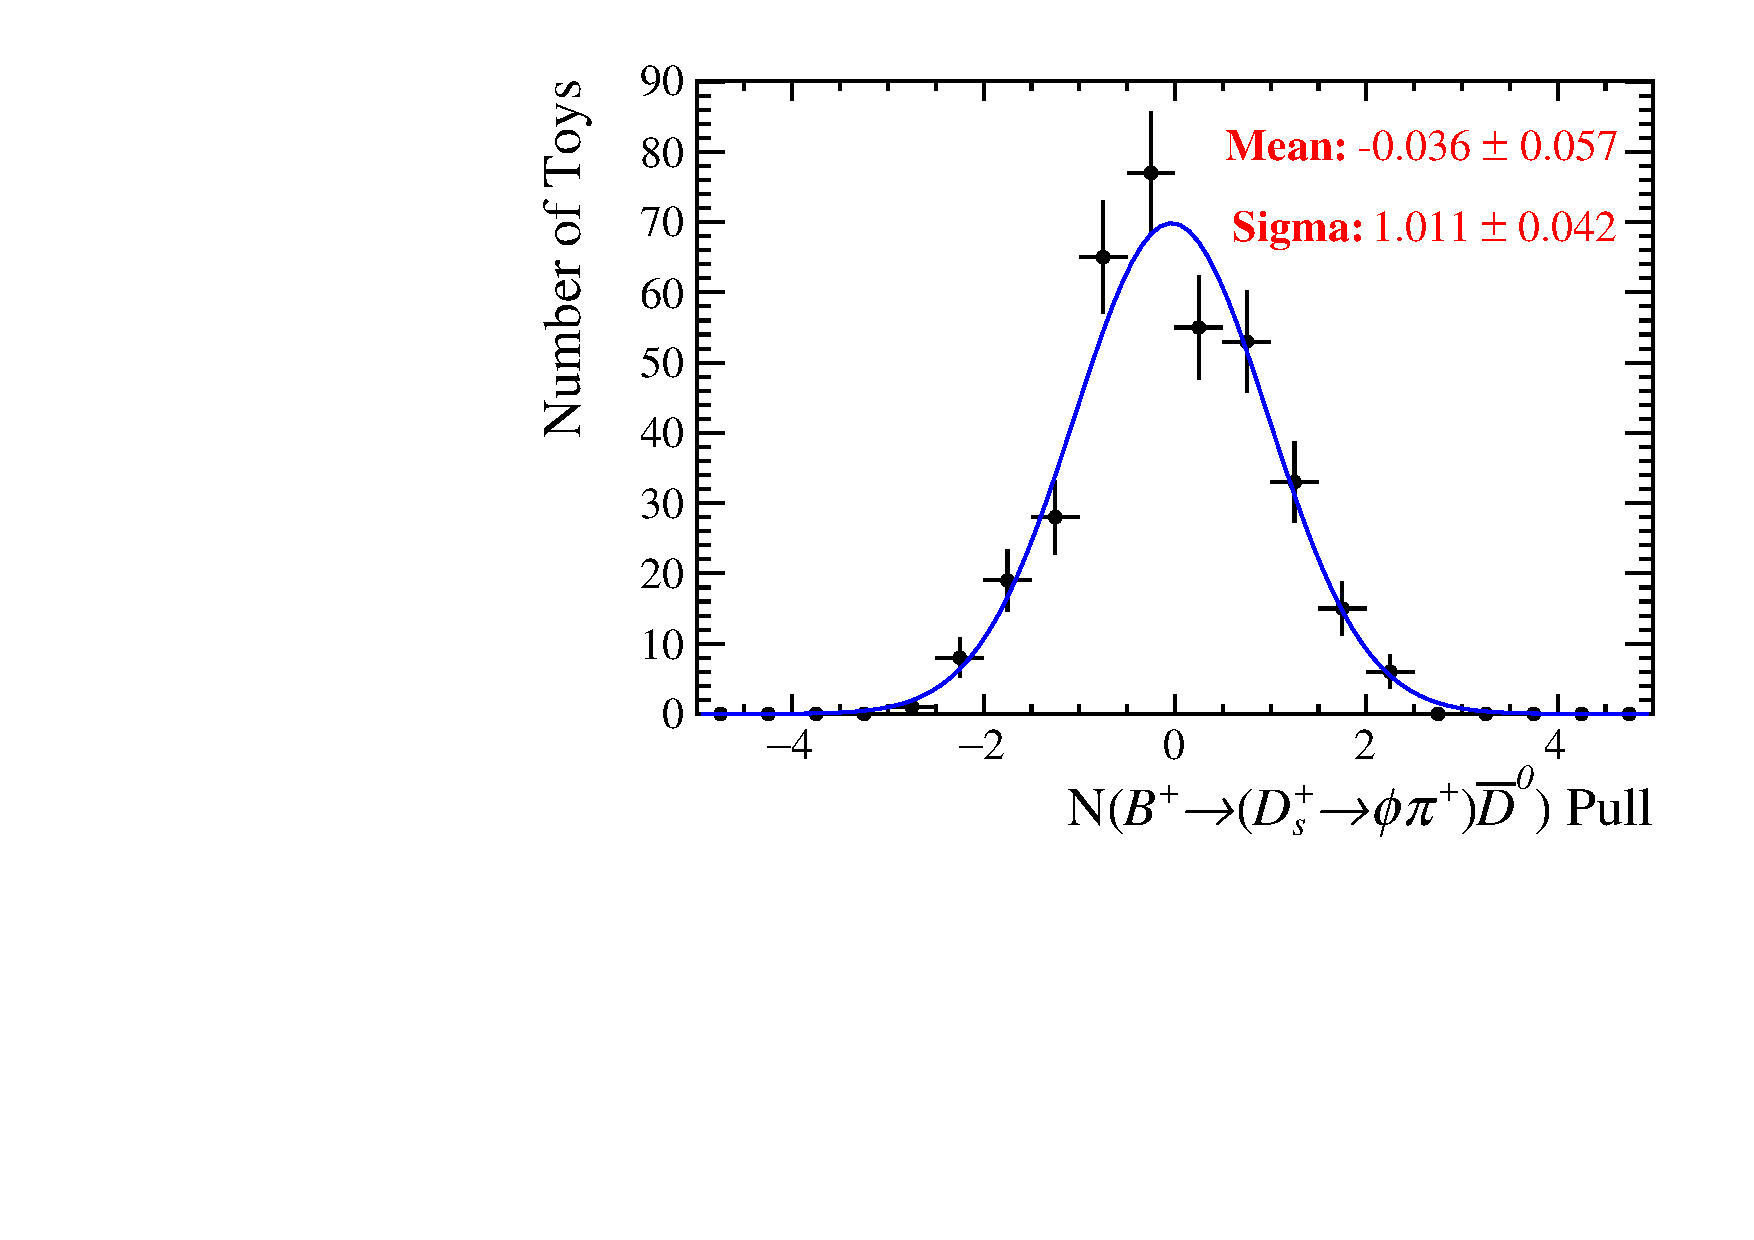
\includegraphics[width=0.32\textwidth]{figs/B2DsPhi/Plots_DsKK_Pull_yield_peak_DsD0_Ds2PhiPi_toy_both_DsBDTbin1_PhiBDTbin1_both_both.pdf}
%       \caption{\decay{\Dsp}{\phiz\pip}}
%    \end{subfigure}\\
%    \begin{subfigure}[t]{1.0\textwidth}
%       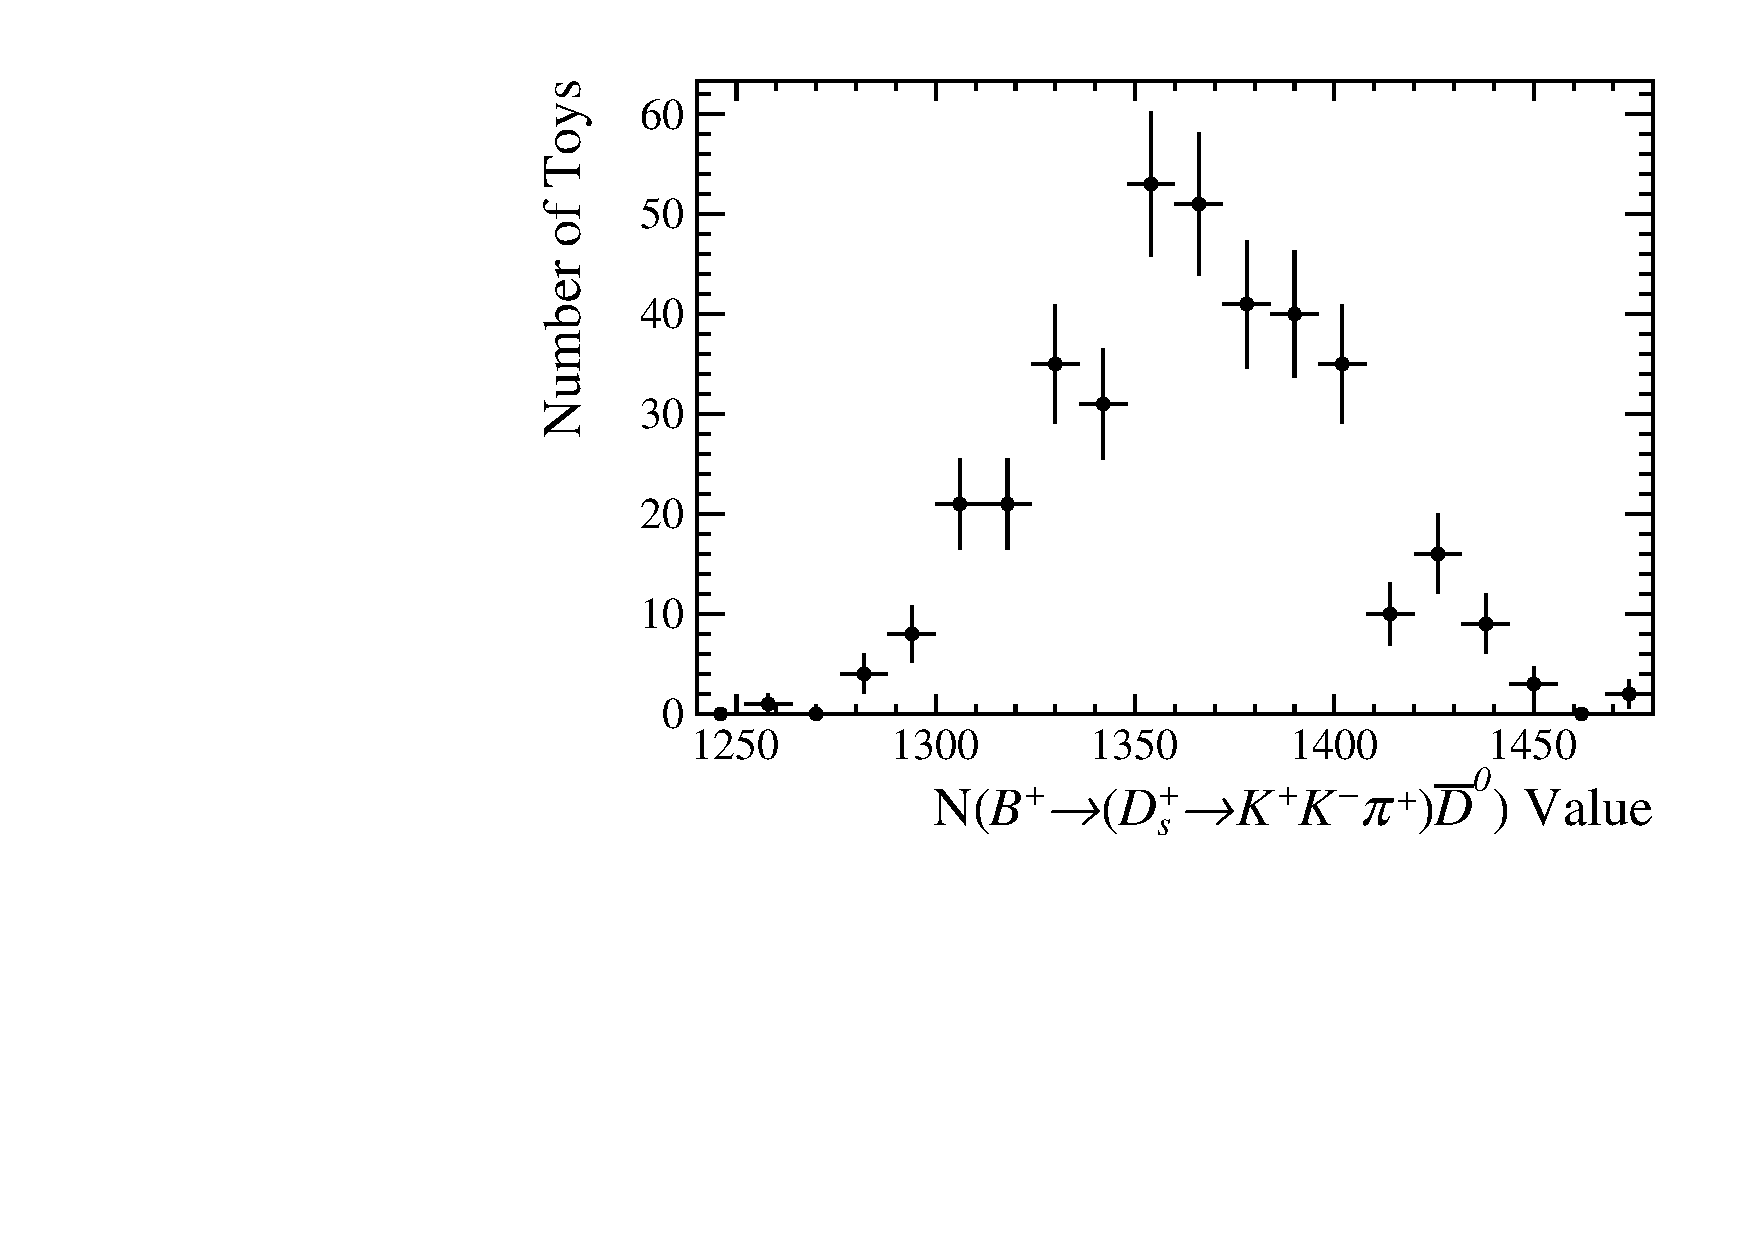
\includegraphics[width=0.32\textwidth]{figs/B2DsPhi/Plots_DsKK_Value_yield_peak_DsD0_Ds2KKPi_toy_both_DsBDTbin1_PhiBDTbin1_both_both.pdf}
%       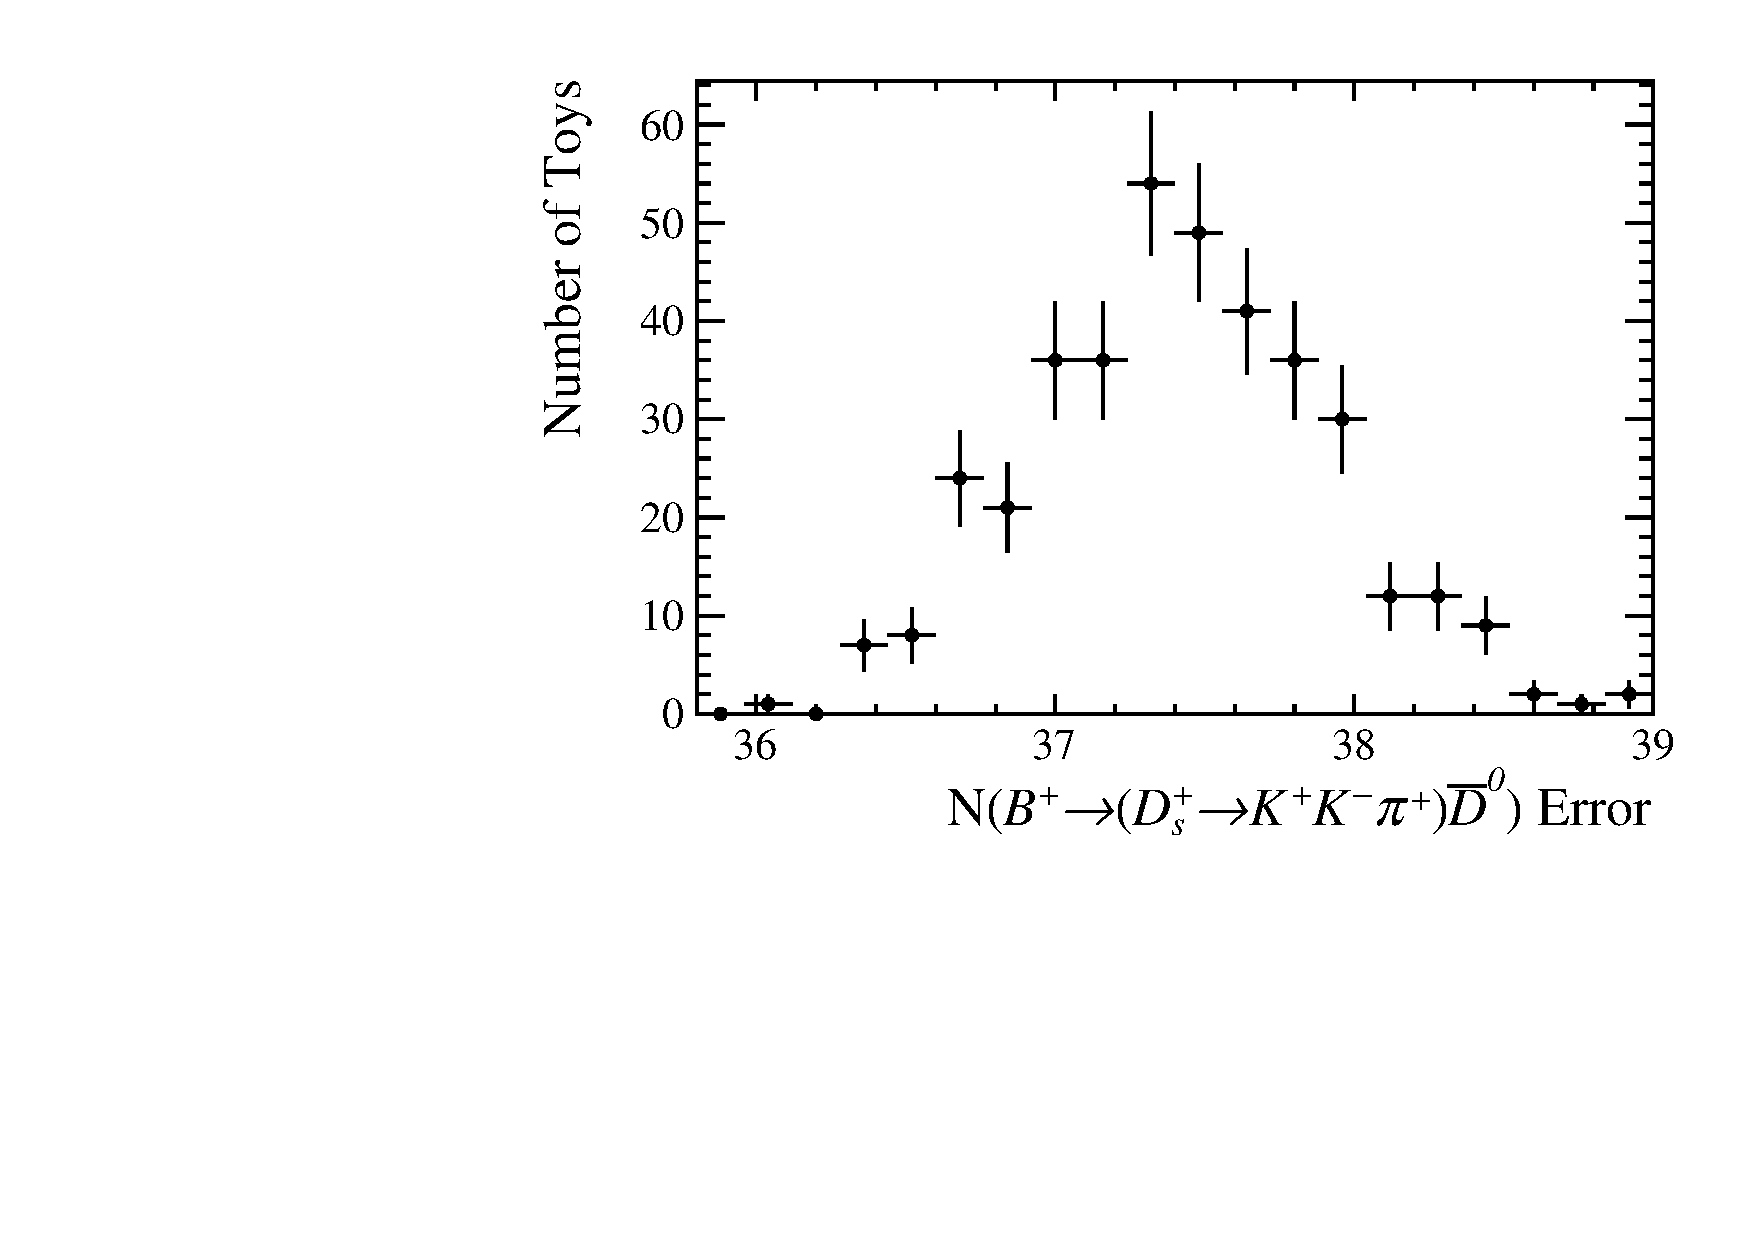
\includegraphics[width=0.32\textwidth]{figs/B2DsPhi/Plots_DsKK_Error_yield_peak_DsD0_Ds2KKPi_toy_both_DsBDTbin1_PhiBDTbin1_both_both.pdf}
%       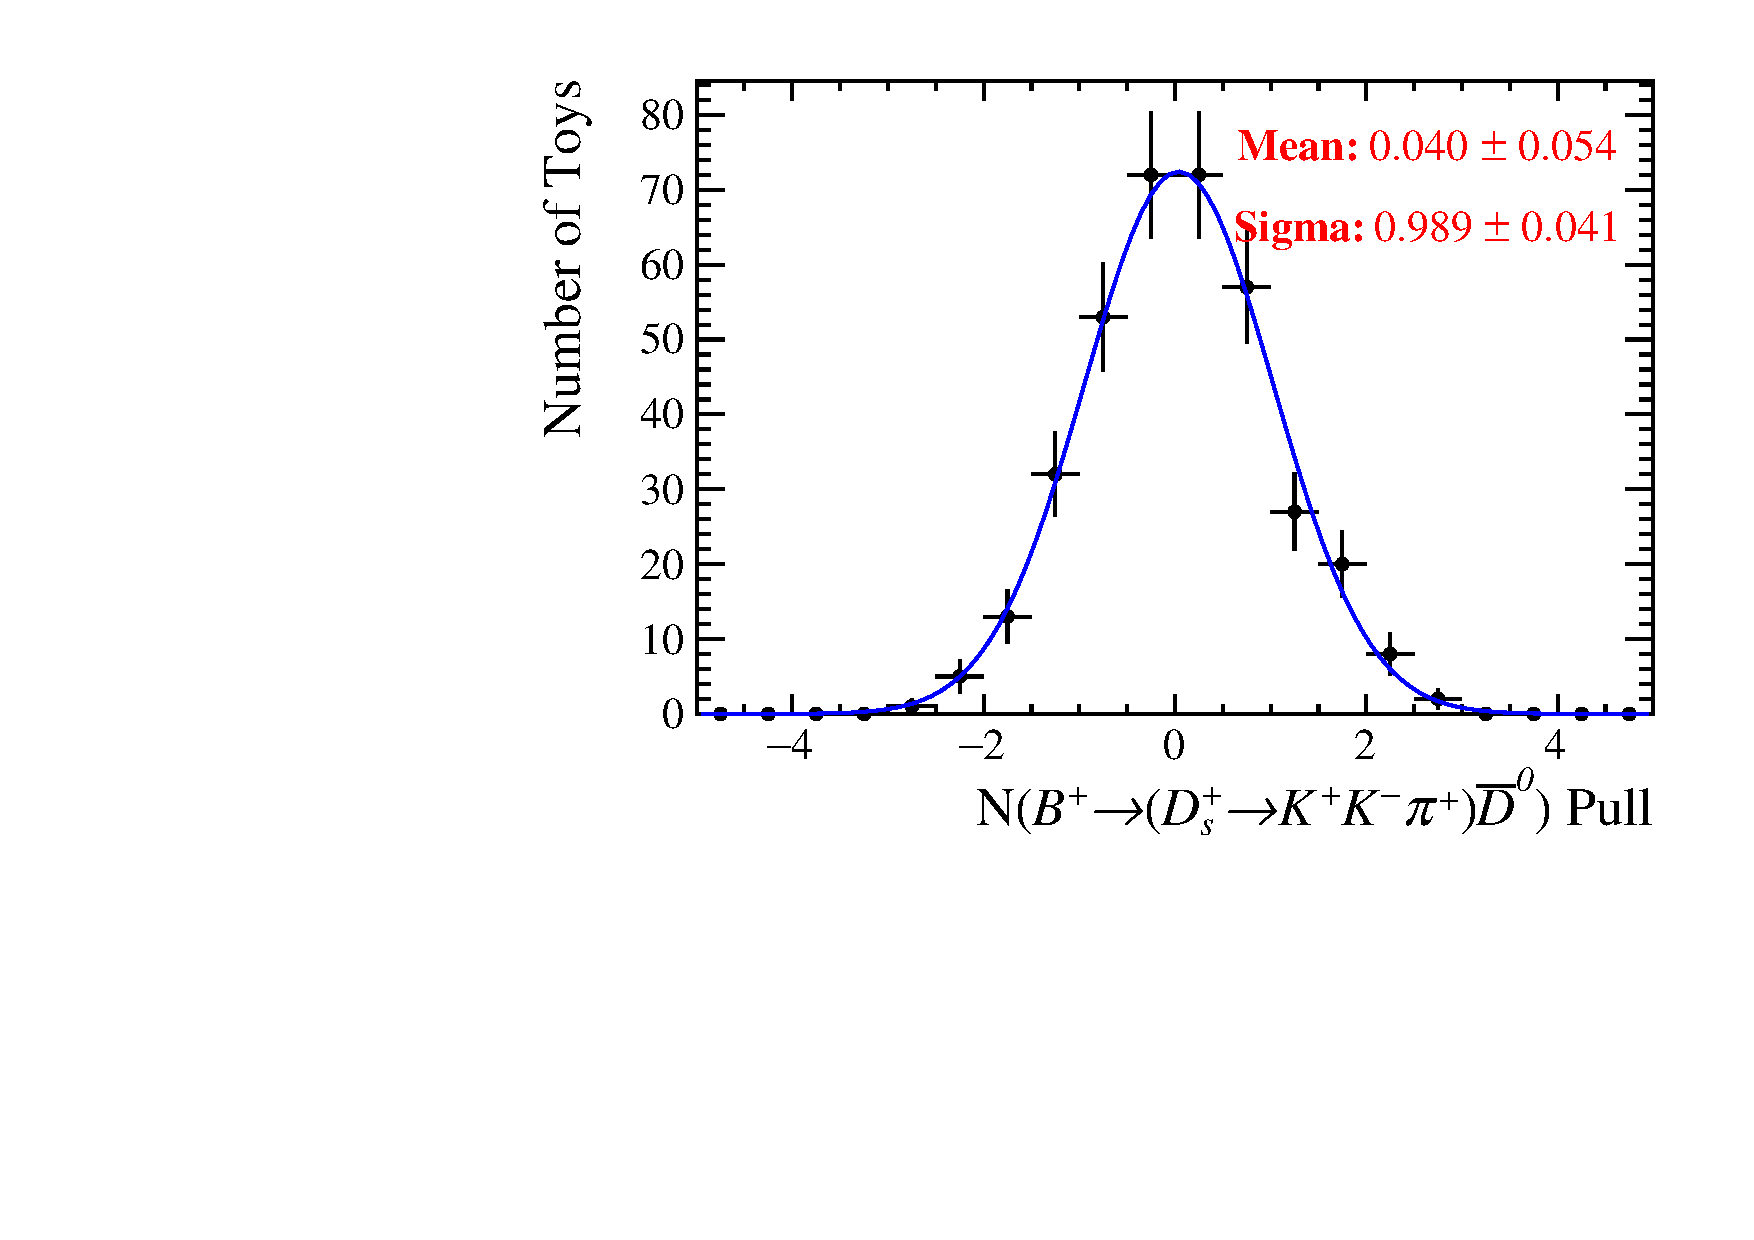
\includegraphics[width=0.32\textwidth]{figs/B2DsPhi/Plots_DsKK_Pull_yield_peak_DsD0_Ds2KKPi_toy_both_DsBDTbin1_PhiBDTbin1_both_both.pdf}
%       \caption{\decay{\Dsp}{\Kp\Km\pip}}
%    \end{subfigure}\\
%    \begin{subfigure}[t]{1.0\textwidth}
%       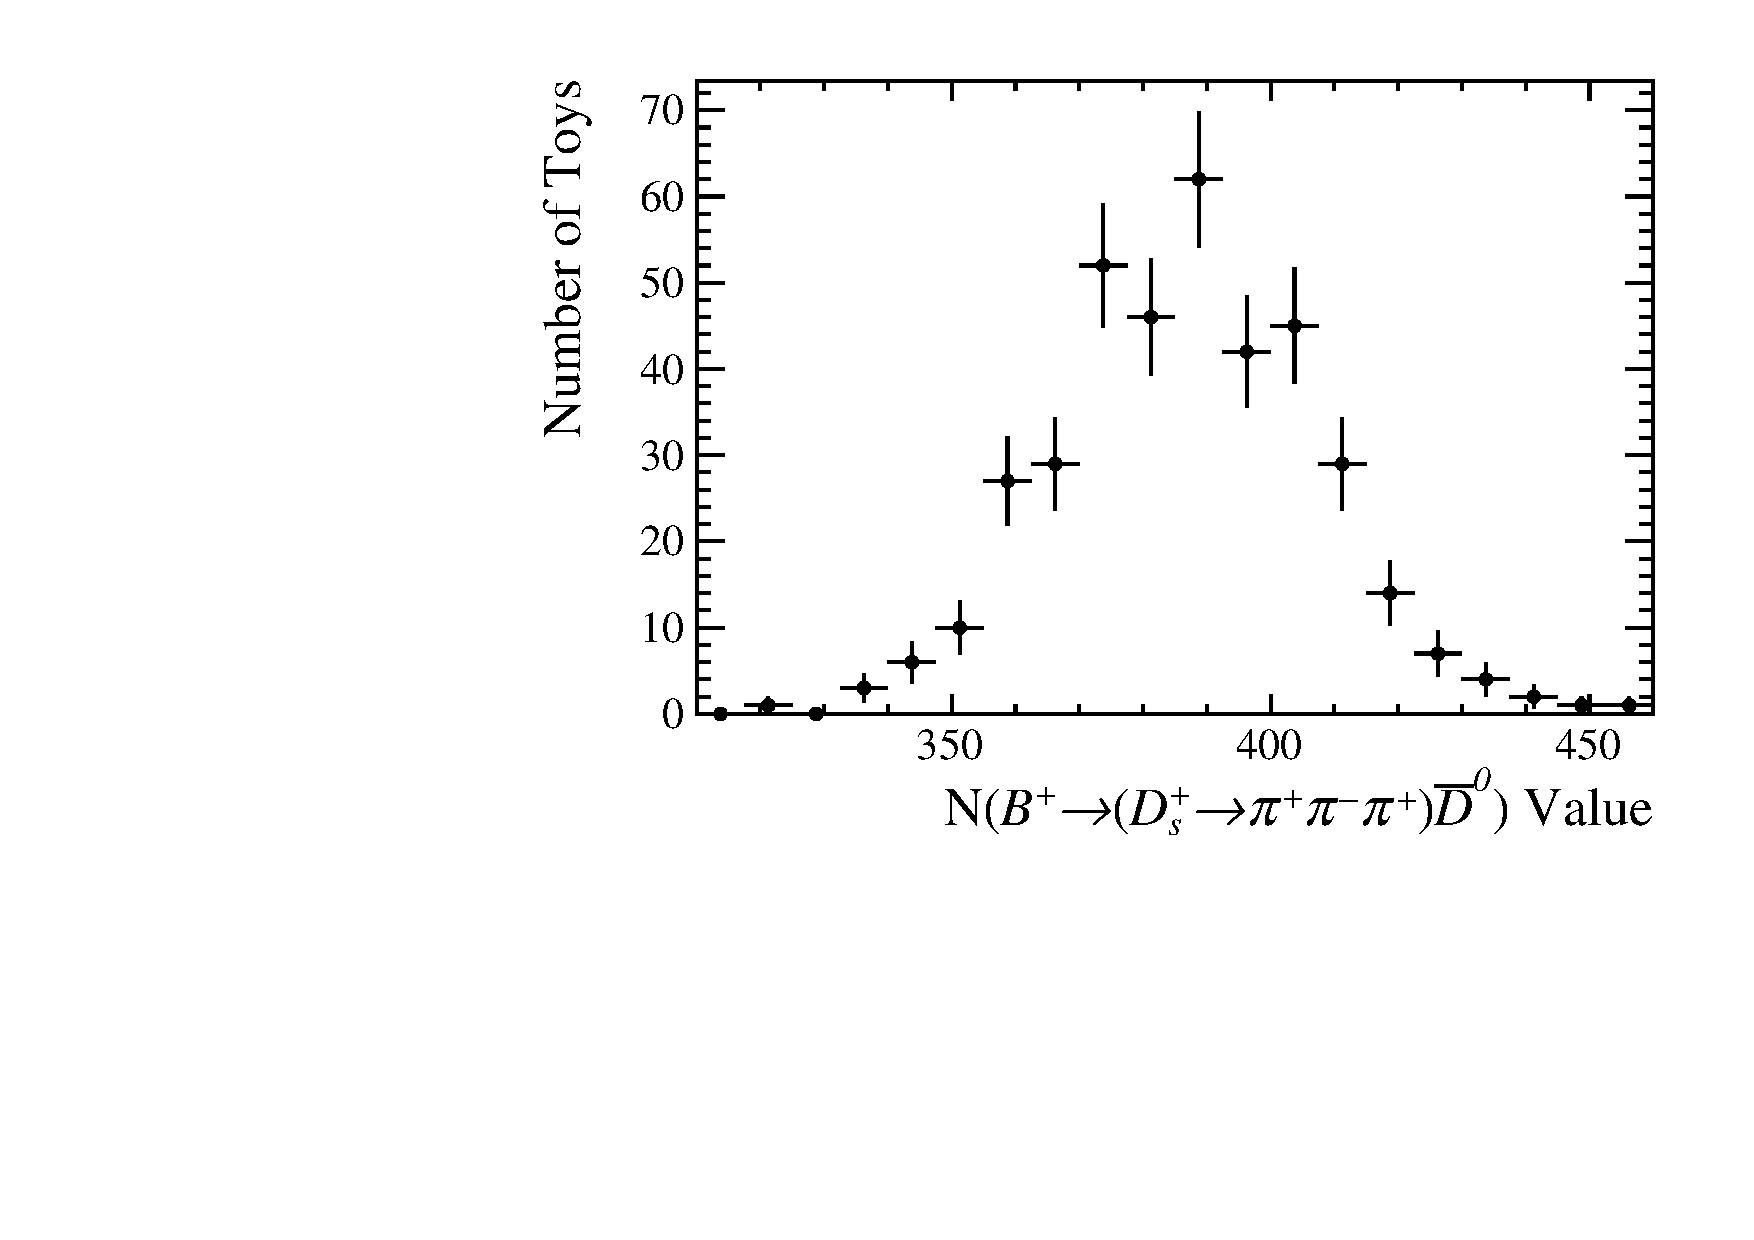
\includegraphics[width=0.32\textwidth]{figs/B2DsPhi/Plots_DsKK_Value_yield_peak_DsD0_Ds2PiPiPi_toy_both_DsBDTbin1_PhiBDTbin1_both_both.pdf}
%       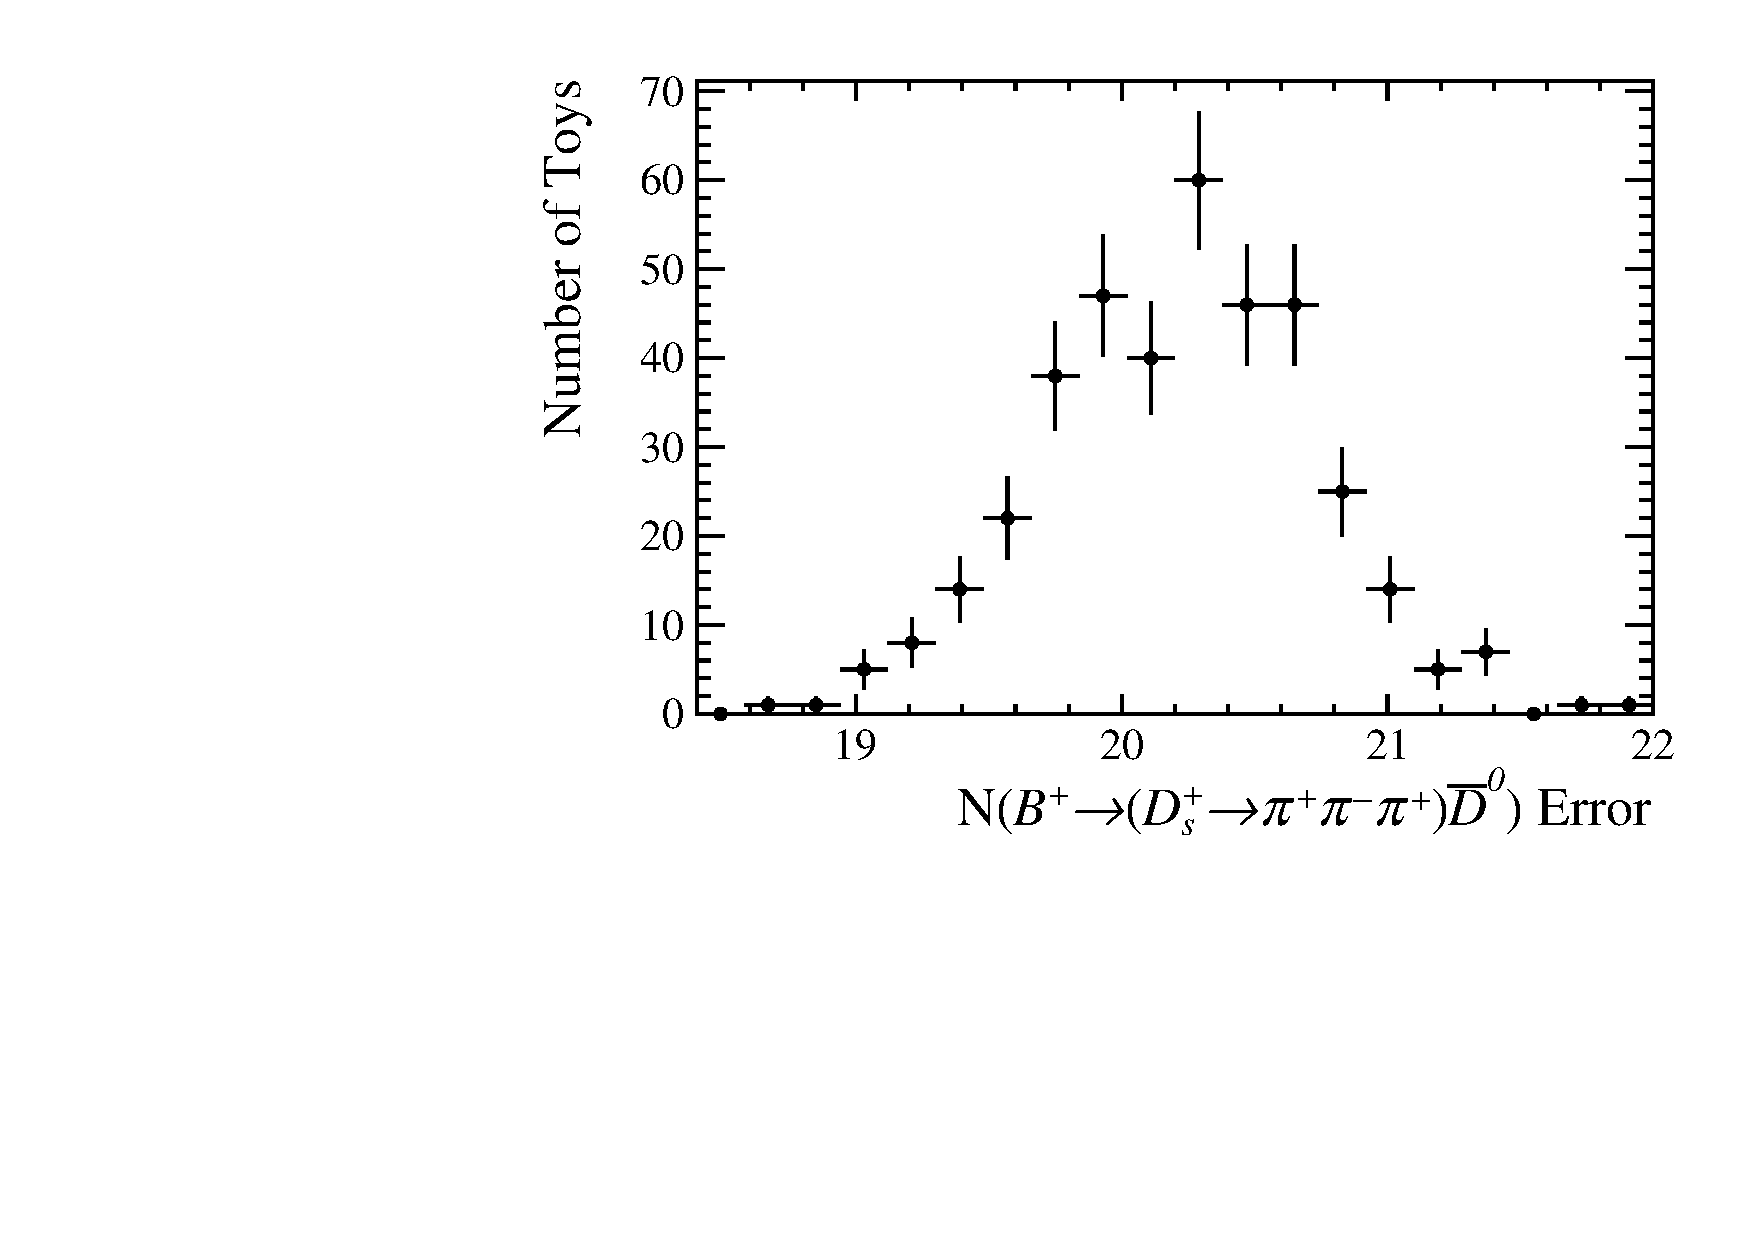
\includegraphics[width=0.32\textwidth]{figs/B2DsPhi/Plots_DsKK_Error_yield_peak_DsD0_Ds2PiPiPi_toy_both_DsBDTbin1_PhiBDTbin1_both_both.pdf}
%       \includegraphics[width=0.32\textwidth]{figs/B2DsPhi/Plots_DsKK_Pull_yield_peak_DsD0_Ds2PiPiPi_toy_both_DsBDTbin1_PhiBDTbin1_both_both.pdf}
%       \caption{\decay{\Dsp}{\pip\pim\pip}}
%    \end{subfigure}\\
%    \begin{subfigure}[t]{1.0\textwidth}
%       \includegraphics[width=0.32\textwidth]{figs/B2DsPhi/Plots_DsKK_Value_yield_peak_DsD0_Ds2KPiPi_toy_both_DsBDTbin1_PhiBDTbin1_both_both.pdf}
%       \includegraphics[width=0.32\textwidth]{figs/B2DsPhi/Plots_DsKK_Error_yield_peak_DsD0_Ds2KPiPi_toy_both_DsBDTbin1_PhiBDTbin1_both_both.pdf}
%       \includegraphics[width=0.32\textwidth]{figs/B2DsPhi/Plots_DsKK_Pull_yield_peak_DsD0_Ds2KPiPi_toy_both_DsBDTbin1_PhiBDTbin1_both_both.pdf}
%       \caption{\decay{\Dsp}{\Kp\pim\pip}}
%    \end{subfigure}

%    \caption{The yield, error and pull distributions for the normalisation channel.}
%    \label{fig:B2DsPhi_Pulls_normalisation}
% \end{figure}
% %%%%%%%%%%%%%%%%%%%%%%%%%%%%%%%%%%%%%%%%%%%%%%%%%%%%%%%%%%


% Similarly, the distributions of the signal yield, error and pull for each of the different \Dsp decay modes are shown in Fig.~\ref{fig:B2DsPhi_Pulls_signal}. The pull means and widths are all within $2\sigma$ of zero and one respectively.


% %%%%%%%%%%%%%%%%%%%%%%%%%%%%%%%%%%%%%%%%%%%%%%%%%%%%%%%%%%
% \begin{figure}[!h]
%    \centering
%    \begin{subfigure}[t]{1.0\textwidth}
%       \includegraphics[width=0.32\textwidth]{figs/B2DsPhi/Plots_DsKK_Value_yield_peak_total_DsPhi_Ds2PhiPi_toy_both_DsBDTbin1_PhiBDTbin1_both_both.pdf}
%       \includegraphics[width=0.32\textwidth]{figs/B2DsPhi/Plots_DsKK_Error_yield_peak_total_DsPhi_Ds2PhiPi_toy_both_DsBDTbin1_PhiBDTbin1_both_both.pdf}
%       \includegraphics[width=0.32\textwidth]{figs/B2DsPhi/Plots_DsKK_Pull_yield_peak_total_DsPhi_Ds2PhiPi_toy_both_DsBDTbin1_PhiBDTbin1_both_both.pdf}
%       \caption{\decay{\Dsp}{\phiz\pip}}
%    \end{subfigure}\\
%    \begin{subfigure}[t]{1.0\textwidth}
%       \includegraphics[width=0.32\textwidth]{figs/B2DsPhi/Plots_DsKK_Value_yield_peak_total_DsPhi_Ds2KKPi_toy_both_DsBDTbin1_PhiBDTbin1_both_both.pdf}
%       \includegraphics[width=0.32\textwidth]{figs/B2DsPhi/Plots_DsKK_Error_yield_peak_total_DsPhi_Ds2KKPi_toy_both_DsBDTbin1_PhiBDTbin1_both_both.pdf}
%       \includegraphics[width=0.32\textwidth]{figs/B2DsPhi/Plots_DsKK_Pull_yield_peak_total_DsPhi_Ds2KKPi_toy_both_DsBDTbin1_PhiBDTbin1_both_both.pdf}
%       \caption{\decay{\Dsp}{\Kp\Km\pip}}
%    \end{subfigure}\\
%    \begin{subfigure}[t]{1.0\textwidth}
%       \includegraphics[width=0.32\textwidth]{figs/B2DsPhi/Plots_DsKK_Value_yield_peak_total_DsPhi_Ds2PiPiPi_toy_both_DsBDTbin1_PhiBDTbin1_both_both.pdf}
%       \includegraphics[width=0.32\textwidth]{figs/B2DsPhi/Plots_DsKK_Error_yield_peak_total_DsPhi_Ds2PiPiPi_toy_both_DsBDTbin1_PhiBDTbin1_both_both.pdf}
%       \includegraphics[width=0.32\textwidth]{figs/B2DsPhi/Plots_DsKK_Pull_yield_peak_total_DsPhi_Ds2PiPiPi_toy_both_DsBDTbin1_PhiBDTbin1_both_both.pdf}
%       \caption{\decay{\Dsp}{\pip\pim\pip}}
%    \end{subfigure}\\
%    \begin{subfigure}[t]{1.0\textwidth}
%       \includegraphics[width=0.32\textwidth]{figs/B2DsPhi/Plots_DsKK_Value_yield_peak_total_DsPhi_Ds2KPiPi_toy_both_DsBDTbin1_PhiBDTbin1_both_both.pdf}
%       \includegraphics[width=0.32\textwidth]{figs/B2DsPhi/Plots_DsKK_Error_yield_peak_total_DsPhi_Ds2KPiPi_toy_both_DsBDTbin1_PhiBDTbin1_both_both.pdf}
%       \includegraphics[width=0.32\textwidth]{figs/B2DsPhi/Plots_DsKK_Pull_yield_peak_total_DsPhi_Ds2KPiPi_toy_both_DsBDTbin1_PhiBDTbin1_both_both.pdf}
%       \caption{\decay{\Dsp}{\Kp\pim\pip}}
%    \end{subfigure}

%    \caption{The yield, error and pull distributions for the signal channel.}
%    \label{fig:B2DsPhi_Pulls_signal}
% \end{figure}
% %%%%%%%%%%%%%%%%%%%%%%%%%%%%%%%%%%%%%%%%%%%%%%%%%%%%%%%%%%

% These distributions were generated using pseudo-experiments in which the yields for each \Dsp mode were free variables rather than being determined using a single free branching fraction parameter.

% The model is also studied using a single branching fraction $\BF(\decay{\Bp}{\Dsp\phiz})$ that determines the yields in each signal mode. This parameter is calculated directly in the fit so it can be assessed for any possible bias. The distribution of the measured values, uncertainties and pulls are shown in Fig.~\ref{fig:B2DsPhi_Pulls_signal}.


% %%%%%%%%%%%%%%%%%%%%%%%%%%%%%%%%%%%%%%%%%%%%%%%%%%%%%%%%%%
% \begin{figure}[!h]
%    \centering
%    \begin{subfigure}[t]{1.0\textwidth}
%       \includegraphics[width=0.32\textwidth]{figs/B2DsPhi/Plots_DsKK_Error_Branching_fraction.pdf}
%       \includegraphics[width=0.32\textwidth]{figs/B2DsPhi/Plots_DsKK_Error_Branching_fraction.pdf}
%       \includegraphics[width=0.32\textwidth]{figs/B2DsPhi/Plots_DsKK_Pull_Branching_fraction.pdf}
%    \end{subfigure}
%    \caption{The branching fraction, error and pull distributions for the full simultaneous fit. The branching fraction is generated assuming the value obtained in the fit to data.}
%    \label{fig:B2DsPhi_Pulls_signal}
% \end{figure}
% %%%%%%%%%%%%%%%%%%%%%%%%%%%%%%%%%%%%%%%%%%%%%%%%%%%%%%%%%%
% The pull mean and width are both within $2\sigma$ of zero and one respectively. 
% As no significant biases are observed in the pulls of any of the yields or branching fraction no corrections are applied to the values determined fit.


\section{Normalisation and signal fits}

The result of the simultaneous fit to the signal and normalisation decays is shown in Figs.~\ref{fig:B2DsPhi_Norm_Fit} and \ref{fig:B2DsPhi_Signal_Fit}. These figures show the distribution of candidates passing all selection requirements along with the total PDF model resulting from the minimisation of the log-likelihood. The four \Dsp decay mode categories have been merged into a single distribution. The fits in each different \Ds decay mode category can be found in Appendix~\ref{ch:appendix_fits}.



%%%%%%%%%%%%%%%%%%%%%%%%%%%%%%%%%%%%%%%%%%%%%%%%%%%%%%%%%%
\begin{figure}[!h]
    \centering
    \begin{subfigure}[t]{1.0\textwidth}
        \includegraphics[width=1.0\textwidth]{figs/Appendix_FitCategories/canvas_DsD0_merged_both_summed_splitHel_splitKKPi_s21_s21r1_s24_s26.pdf}
    \end{subfigure}
    \caption{Invariant mass fit to \decay{\Bp}{\Dsp\Dzb} candidates}
    \label{fig:B2DsPhi_Norm_Fit}
\end{figure}
%%%%%%%%%%%%%%%%%%%%%%%%%%%%%%%%%%%%%%%%%%%%%%%%%%%%%%%%%%

The high purity of the normalisation mode reconstruction can be seen in Fig.~\ref{fig:B2DsPhi_Norm_Fit}, as the contribution from the combinatorial background shape is very small. Additionally, the double-peaked structure of the partially reconstructed \decay{\Bp}{\Dssp\Dzb} and \decay{\Bp}{\Dsp\Dstarzb} decays is clearly visible. 
%The decays are split into two $\cos\theta_{K}$ categories, 


%%%%%%%%%%%%%%%%%%%%%%%%%%%%%%%%%%%%%%%%%%%%%%%%%%%%%%%%%%
\begin{figure}[!h]
    \centering
    \begin{subfigure}[t]{1.0\textwidth}
        \includegraphics[width=1.0\textwidth]{figs/B2DsPhi/Fig4a.eps}
    \end{subfigure}
    \begin{subfigure}[t]{1.0\textwidth}
        \includegraphics[width=1.0\textwidth]{figs/B2DsPhi/Fig4b.eps}
    \end{subfigure}
    \caption{Invariant mass fit to \decay{\Bp}{\Dsp\phiz} candidates}
    \label{fig:B2DsPhi_Signal_Fit}
\end{figure}
%%%%%%%%%%%%%%%%%%%%%%%%%%%%%%%%%%%%%%%%%%%%%%%%%%%%%%%%%%

The fit to the signal mode is shown in Fig.~\ref{fig:B2DsPhi_Signal_Fit}. This figure includes the \decay{\Bp}{\Dsp\phiz} candidates in both the $|m(\Kp\Km)| < 10\mevcc$ (\phiz-region) and $10< |m(\Kp\Km)| < 40\mevcc$ (\phiz-sideband) categories. These are further split into the two $\cos\theta_{K}$ categories in an analogous way to the normalisation decays.



The final values of the parameters as determined by the fit are tabulated in Table~\ref{tab:B2DsPhi_free_variables}, including the branching fraction $\BF(\decay{\Bp}{\Dsp\phiz})$. This parameter includes a correction to account for the efficiencies of the signal and normalisation modes as discussed in Sec.~\ref{sec:B2DsPhi_effcorrections}. 

\begin{longtable}{ l l c }
\hline
Type       & Parameter                                                                    & Fit result\\
\hline
POI        & Branching fraction $\BF(\decay{\Bp}{\Dsp\phiz}) (\times 10^{-7})$            &   $\mathbf{1.17^{+ 1.56}_{-1.37} }$\\
\hline
Shape      & Combinatorial slope $c$                                                      &   $(-3.3^{+0.4}_{-0.4})\times10^{-3}$\\
           & Mean \Bp mass (\mevcc)                                                       &   $5279.10^{+0.17}_{-0.17} $\\
           & Mass offset $\delta$ (\mevcc)                                                &   $-1.975^{+0.362}_{-0.362} $\\
           & Relative heights $\xi$                                                       &   $0.68^{+0.05}_{-0.05} $\\
           & $\sigma_{1}$ for \decay{\Dsp}{\Kp\Km\pip}  (\mevcc)                          &   $7.61^{+0.18}_{-0.18} $\\
           & $\sigma_{1}$ for \decay{\Dsp}{\Kp\pim\pip} (\mevcc)                          &   $8.77^{+0.59}_{-0.55} $\\
           & $\sigma_{1}$ for \decay{\Dsp}{\phiz\pip}  (\mevcc)                           &   $7.53^{+0.22}_{-0.21} $\\
           & $\sigma_{1}$ for \decay{\Dsp}{\pip\pim\pip}  (\mevcc)                        &   $8.30^{+0.36}_{-0.34} $\\
\hline
Yields     & $N(\decay{\Bp}{(\decay{\Dsp}{\Kp\Km\pip}  )\Dzb})$                           &   $1324^{+37}_{-36} $\\
           & $N(\decay{\Bp}{(\decay{\Dsp}{\Kp\pim\pip} )\Dzb})$                           &   $182^{+14}_{-13} $\\
           & $N(\decay{\Bp}{(\decay{\Dsp}{\phiz\pip}   )\Dzb})$                           &   $801^{+29}_{-28} $\\
           & $N(\decay{\Bp}{(\decay{\Dsp}{\pip\pim\pip})\Dzb})$                           &   $369^{+20}_{-19} $\\
           & $N(\Dssp\Dzb + \Dsp\Dstarzb)$ in \decay{\Dsp}{\Kp\Km\pip}                    &   $2827^{+52}_{-51} $\\
           & $N(\Dssp\Dzb + \Dsp\Dstarzb)$ in \decay{\Dsp}{\Kp\pim\pip}                   &   $394^{+20}_{-20} $\\
           & $N(\Dssp\Dzb + \Dsp\Dstarzb)$ in \decay{\Dsp}{\phiz\pip}                     &   $1733^{+38}_{-37} $\\
           & $N(\Dssp\Dzb + \Dsp\Dstarzb)$ in \decay{\Dsp}{\pip\pim\pip}                  &   $804^{+25}_{-25} $\\
           & $N(\Dssp\phiz + D_{s}^{(*)+}\Km\Kstarz)$ in \decay{\Dsp}{\Kp\Km\pip}         &   $139^{+19}_{-20} $\\
           & $N(\Dssp\phiz + D_{s}^{(*)+}\Km\Kstarz)$ in \decay{\Dsp}{\Kp\pim\pip}        &   $7^{+4}_{-4} $\\
           & $N(\Dssp\phiz + D_{s}^{(*)+}\Km\Kstarz)$ in \decay{\Dsp}{\phiz\pip}          &   $67^{+10}_{-10} $\\
           & $N(\Dssp\phiz + D_{s}^{(*)+}\Km\Kstarz)$ in \decay{\Dsp}{\Kp\pim\pip}        &   $25^{+7}_{-6} $\\

           & $N_{\text{comb}}(\Dsp\Dzb)$ \decay{\Dsp}{\Kp\Km\pip} in H1                   &   $112^{+30}_{-25} $\\
           & $N_{\text{comb}}(\Dsp\Dzb)$ \decay{\Dsp}{\Kp\Km\pip} in H2                   &   $50^{+17}_{-14} $\\
           & $N_{\text{comb}}(\Dsp\Dzb)$ \decay{\Dsp}{\Kp\pim\pip} in H1                  &   $71^{+20}_{-17} $\\
           & $N_{\text{comb}}(\Dsp\Dzb)$ \decay{\Dsp}{\Kp\pim\pip} in H2                  &   $41^{+12}_{-10} $\\
           & $N_{\text{comb}}(\Dsp\Dzb)$ \decay{\Dsp}{\phiz\pip} in H1                    &   $31^{+14}_{-11} $\\
           & $N_{\text{comb}}(\Dsp\Dzb)$ \decay{\Dsp}{\phiz\pip} in H2                    &   $12^{+9}_{-6} $\\
           & $N_{\text{comb}}(\Dsp\Dzb)$ \decay{\Dsp}{\pip\pim\pip} in H1                 &   $41^{+14}_{-11} $\\
           & $N_{\text{comb}}(\Dsp\Dzb)$ \decay{\Dsp}{\pip\pim\pip} in H2                 &   $35^{+14}_{-11} $\\
           & $N_{\text{comb}}(\Dsp\phiz)$ \decay{\Dsp}{\Kp\Km\pip} in H1                  &   $107^{+23}_{-20} $\\
           & $N_{\text{comb}}(\Dsp\phiz)$ \decay{\Dsp}{\Kp\Km\pip} in H2                  &   $52^{+12}_{-11} $\\
           & $N_{\text{comb}}(\Dsp\phiz)$ \decay{\Dsp}{\Kp\pim\pip} in H1                 &   $19^{+7}_{-6} $\\
           & $N_{\text{comb}}(\Dsp\phiz)$ \decay{\Dsp}{\Kp\pim\pip} in H2                 &   $18^{+5}_{-4} $\\
           & $N_{\text{comb}}(\Dsp\phiz)$ \decay{\Dsp}{\phiz\pip} in H1                   &   $38^{+14}_{-12} $\\
           & $N_{\text{comb}}(\Dsp\phiz)$ \decay{\Dsp}{\phiz\pip} in H2                   &   $27^{+8}_{-7} $\\
           & $N_{\text{comb}}(\Dsp\phiz)$ \decay{\Dsp}{\pip\pim\pip} in H1                &   $42^{+10}_{-9} $\\
           & $N_{\text{comb}}(\Dsp\phiz)$ \decay{\Dsp}{\pip\pim\pip} in H2                &   $25^{+7}_{-6} $\\
           & $N_{\text{comb}}(\Dsp\phiz)$ \phiz-sideband \decay{\Dsp}{\Kp\Km\pip} in H1   &   $33^{+13}_{-10} $\\
           & $N_{\text{comb}}(\Dsp\phiz)$ \phiz-sideband \decay{\Dsp}{\Kp\Km\pip} in H2   &   $26^{+11}_{-9} $\\
           & $N_{\text{comb}}(\Dsp\phiz)$ \phiz-sideband \decay{\Dsp}{\Kp\pim\pip} in H1  &   $18^{+7}_{-6} $\\
           & $N_{\text{comb}}(\Dsp\phiz)$ \phiz-sideband \decay{\Dsp}{\Kp\pim\pip} in H2  &   $14^{+5}_{-5} $\\
           & $N_{\text{comb}}(\Dsp\phiz)$ \phiz-sideband \decay{\Dsp}{\phiz\pip} in H1    &   $5^{+6}_{-4} $\\
           & $N_{\text{comb}}(\Dsp\phiz)$ \phiz-sideband \decay{\Dsp}{\phiz\pip} in H2    &   $12^{+8}_{-7} $\\
           & $N_{\text{comb}}(\Dsp\phiz)$ \phiz-sideband \decay{\Dsp}{\pip\pim\pip} in H1 &   $16^{+8}_{-6} $\\
           & $N_{\text{comb}}(\Dsp\phiz)$ \phiz-sideband \decay{\Dsp}{\pip\pim\pip} in H2 &   $14^{+8}_{-8} $\\
\hline
Fractions  & Ratio of \Dsp\Kp\Km to \Dsp\Dzb                                              &   $0.024^{+0.004}_{-0.004} $\\
           & Fraction of \Dsp\Km\Kstarz in (\Dssp\Km\Kstarz+\Dsp\Km\Kstarz)               &   $0.664^{+0.046}_{-0.044} $\\
           & Fraction of $\Dssp\phiz$ in ($D_{s}^{(*)+}\Km\Kstarz$ + $\Dssp\phiz$)        &   $0.172^{+0.103}_{-0.135} $\\
           & Ratio of $\Dsp D_{(s)}^{(*)-}$ to ($\Dssp\phiz$ + $D_{s}^{(*)+}\Km\Kstarz$)  &   $0.567^{+0.129}_{-0.107} $\\
           & Fraction of \Dssp\Dzb in (\Dssp\Dzb+\Dsp\Dstarzb) in H1                      &   $0.302^{+0.031}_{-0.031} $\\
           & Fraction of \Dssp\Dzb in (\Dssp\Dzb+\Dsp\Dstarzb) in H2                      &   $0.342^{+0.037}_{-0.037} $\\
           & Fraction of normalisation part reco in H1                                    &   $0.593^{+0.005}_{-0.005} $\\
           & Fraction of normalisation peak in H1                                         &   $0.592^{+0.010}_{-0.010} $\\
           & Ratio of \Dssp\Dstarzb to (\Dssp\Dzb + \Dsp\Dstarzb)                         &   $0.607^{+0.016}_{-0.015} $\\
\hline
\caption{The fit result with final values of all floating variables used in the fit model. Here H1 and H2 represent the $|\cos\theta_{K}|>0.4$ and $|\cos\theta_{K}|<0.4$ categories respectively.} 
\label{tab:B2DsPhi_free_variables} 
\end{longtable}


\section{Efficiency corrections}
\label{sec:B2DsPhi_effcorrections}

The branching fraction for \decay{\Bp}{\Dsp\phiz} decays is determined by correcting the yields for the signal and normalisation channels by their respective efficiencies. 
%In determining the efficiencies both the \decay{\Bp}{\Dsp\phiz} and \decay{\Bp}{\Dsp\Dzb} decays are assumed to be pseudo-two-body decays in which variations as a function of phase-space are negligible. 
%This means the relative efficiency can be calculated as a simple ratio for each \Dsp decay mode, simplifying the correction considerably.    
The relative efficiency are calculated as a ratio for each \Dsp decay mode.    

The efficiencies for each stage of selection are either determined from the appropriate simulation samples for the signal and normalisation decays, or from dedicated calibration data samples for the efficiencies involving particle identification requirements. 
Each set of efficiencies are determined with respect to the previous one, such that the total efficiency is given by the product of each of them.


\subsection{Efficiencies from simulation}

The efficiencies for each step of selection are listed separately for the different \Dsp decay modes in Table~\ref{tab:B2DsPhi_eff}. 
%These steps are closely related to the stages previously described in Chapter~\ref{ch:selection}, however more specific details of what is included in each step is described here. 
The efficiencies are calculated separately for the different years of data taking, however they are combined here, weighting according to the relative contributions to the total data set. 

% \begin{table}[h]
% \centering
% \begin{tabular}{ l c c c }

% \hline
% Requirement             & $\epsilon(\decay{\Bp}{\Dsp\Dzb})$  & $\epsilon(\decay{\Bp}{\Dsp\phiz})$ & Ratio \\ 
% \hline
% Acceptance              & 17.42 $\pm$ 0.03         & 18.35 $\pm$ 0.04      & 0.950 $\pm$ 0.003  \\
% Reconstruction          &  2.11 $\pm$ 0.02         &  1.96 $\pm$ 0.02      & 1.077 $\pm$ 0.013  \\
% Trigger                 & 17.78 $\pm$ 0.04         & 18.63 $\pm$ 0.04      & 0.954 $\pm$ 0.003  \\
% Mass window             & 17.78 $\pm$ 0.04         & 18.63 $\pm$ 0.04      & 0.954 $\pm$ 0.003  \\
% Vetoes                  & 17.78 $\pm$ 0.04         & 18.63 $\pm$ 0.04      & 0.954 $\pm$ 0.003  \\
% $\chi^{2}_{\text{IP}}$  & 17.78 $\pm$ 0.04         & 18.63 $\pm$ 0.04      & 0.954 $\pm$ 0.003  \\
% Charmless               & 17.78 $\pm$ 0.04         & 18.63 $\pm$ 0.04      & 0.954 $\pm$ 0.003  \\
% \hline
% \end{tabular}
% \caption{Efficiencies (in \%) determined from simulation samples for \decay{\Dsp}{\Kp\Km\pip} decays and the ratio $\epsilon(\decay{\Bp}{\Dsp\Dzb})/\epsilon(\decay{\Bp}{\Dsp\phiz})$. The errors are statistical.} 
% \label{tab:B2DsPhi_eff_KKPi} 
% \end{table}

% KKPi   17.42352941    0.034705882    18.34588235    0.035588235    0.9495      0.002558824
% KKPi  2.111764706    0.02     1.958823529    0.015588235    1.077323529    0.013117647

% \begin{table}[h]
% \centering
% \begin{tabular}{ l c c c }

% \hline
% Requirement             & $\epsilon(\decay{\Bp}{\Dsp\Dzb})$  & $\epsilon(\decay{\Bp}{\Dsp\phiz})$ & Ratio \\  
% \hline
% Acceptance              & 16.53 $\pm$ 0.04         & 17.36 $\pm$ 0.04      & 0.952 $\pm$ 0.003  \\
% Reconstruction          & 17.78 $\pm$ 0.04         & 18.63 $\pm$ 0.04      & 0.954 $\pm$ 0.003  \\
% Trigger                 & 17.78 $\pm$ 0.04         & 18.63 $\pm$ 0.04      & 0.954 $\pm$ 0.003  \\
% Mass window             & 17.78 $\pm$ 0.04         & 18.63 $\pm$ 0.04      & 0.954 $\pm$ 0.003  \\
% Vetoes                  & 17.78 $\pm$ 0.04         & 18.63 $\pm$ 0.04      & 0.954 $\pm$ 0.003  \\
% $\chi^{2}_{\text{IP}}$  & 17.78 $\pm$ 0.04         & 18.63 $\pm$ 0.04      & 0.954 $\pm$ 0.003  \\
% Charmless               & 17.78 $\pm$ 0.04         & 18.63 $\pm$ 0.04      & 0.954 $\pm$ 0.003  \\
% \hline
% \end{tabular}
% \caption{Efficiencies (in \%) determined from simulation samples for \decay{\Dsp}{\Kp\pim\pip} decays and the ratio $\epsilon(\decay{\Bp}{\Dsp\Dzb})/\epsilon(\decay{\Bp}{\Dsp\phiz})$. The errors are statistical.} 
% \label{tab:B2DsPhi_eff_KPiPi} 
% \end{table}

% KPiPi  16.52647059    0.035588235    17.36147059    0.035588235    0.951941176    0.002558824
% KPiPi 2.263823529    0.02     2.063823529    0.02     1.095117647    0.014
% \begin{table}[h]
% \centering
% \begin{tabular}{ l c c c }

% \hline
% Requirement             & $\epsilon(\decay{\Bp}{\Dsp\Dzb})$  & $\epsilon(\decay{\Bp}{\Dsp\phiz})$ & Ratio \\   
% \hline
% Acceptance              & 15.91 $\pm$ 0.03         & 16.77 $\pm$ 0.04      & 0.949 $\pm$ 0.003  \\
% Reconstruction          & 17.78 $\pm$ 0.04         & 18.63 $\pm$ 0.04      & 0.954 $\pm$ 0.003  \\
% Trigger                 & 17.78 $\pm$ 0.04         & 18.63 $\pm$ 0.04      & 0.954 $\pm$ 0.003  \\
% Mass window             & 17.78 $\pm$ 0.04         & 18.63 $\pm$ 0.04      & 0.954 $\pm$ 0.003  \\
% Vetoes                  & 17.78 $\pm$ 0.04         & 18.63 $\pm$ 0.04      & 0.954 $\pm$ 0.003  \\
% $\chi^{2}_{\text{IP}}$  & 17.78 $\pm$ 0.04         & 18.63 $\pm$ 0.04      & 0.954 $\pm$ 0.003  \\
% Charmless               & 17.78 $\pm$ 0.04         & 18.63 $\pm$ 0.04      & 0.954 $\pm$ 0.003  \\
% \hline
% \end{tabular}
% \caption{Efficiencies (in \%) determined from simulation samples for \decay{\Dsp}{\pip\pim\pip} decays and the ratio $\epsilon(\decay{\Bp}{\Dsp\Dzb})/\epsilon(\decay{\Bp}{\Dsp\phiz})$. The errors are statistical.} 
% \label{tab:B2DsPhi_eff_PiPiPi} 
% \end{table}

% PiPiPi   15.91264706    0.031764706    16.76882353    0.034705882    0.949088235    0.002558824
% PiPiPi   2.364117647    0.02     2.135    0.02     1.106411765    0.013852941



%%%%%%%
\begin{table}[h]
   \centering
   \begin{tabular}{ l l S[table-format=3.2(3)] S[table-format=3.2(3)] S[table-format=1.3(3)] }
      \hline
      Requirement             & \Dsp mode   & {$\epsilon(\decay{\Bp}{\Dsp\Dzb})$}  & {$\epsilon(\decay{\Bp}{\Dsp\phiz})$} & {Ratio} \\
      \hline
      Acceptance              & $\Kp\Km\pip$      & 17.42 \pm 0.03         & 18.35 \pm 0.04      & 0.950 \pm 0.003  \\
                              & $\Kp\pim\pip$     & 16.53 \pm 0.04         & 17.36 \pm 0.04      & 0.952 \pm 0.003  \\
                              & $\pip\pim\pip$    & 15.91 \pm 0.03         & 16.77 \pm 0.04      & 0.949 \pm 0.003  \\
      \hline
      Reconstruction          & $\Kp\Km\pip$      & 2.11 \pm 0.02         & 1.96 \pm 0.02     & 1.078 \pm 0.013  \\
                              & $\Kp\pim\pip$     & 2.27 \pm 0.02         & 2.06 \pm 0.02     & 1.095 \pm 0.014  \\
                              & $\pip\pim\pip$    & 2.36 \pm 0.02         & 2.13 \pm 0.02     & 1.105 \pm 0.014  \\
      \hline
      Trigger                 & $\Kp\Km\pip$      & 93.3 \pm 0.2         & 93.1 \pm 0.2     & 1.003 \pm 0.003  \\
                              & $\Kp\pim\pip$     & 95.1 \pm 0.2         & 93.5 \pm 0.2     & 1.017 \pm 0.003  \\
                              & $\pip\pim\pip$    & 95.3 \pm 0.2         & 93.7 \pm 0.2     & 1.017 \pm 0.003  \\
      \hline
      Mass window             & $\Kp\Km\pip$      & 96.2 \pm 0.2         & 94.1 \pm 0.2     & 1.022 \pm 0.003  \\
                              & $\Kp\pim\pip$     & 94.9 \pm 0.2         & 94.1 \pm 0.2     & 1.008 \pm 0.003  \\
                              & $\pip\pim\pip$    & 93.7 \pm 0.2         & 92.4 \pm 0.2     & 1.015 \pm 0.004  \\
      \hline
      Vetoes                  & $\Kp\Km\pip$      & 99.9 \pm 0.0         & 95.2 \pm 0.2     & 1.049 \pm 0.002  \\
                              & $\Kp\pim\pip$     & 99.9 \pm 0.0         & 92.4 \pm 0.3     & 1.080 \pm 0.004  \\
                              & $\pip\pim\pip$    & 99.9 \pm 0.0         & 90.3 \pm 0.3     & 1.105 \pm 0.004  \\
      \hline
      Charmless               & $\Kp\Km\pip$      & 72.6 \pm 0.4         & 100.0 \pm 0.0     & 0.726 \pm 0.004  \\
                              & $\Kp\pim\pip$     & 65.8 \pm 0.4         & 63.0 \pm 0.5     & 1.044 \pm 0.011  \\
                              & $\pip\pim\pip$    & 66.0 \pm 0.4         & 82.9 \pm 0.4     & 0.796 \pm 0.006  \\
      \hline
      $\chi^{2}_{\text{IP}}$  & $\Kp\Km\pip$      & 100.0 \pm 0.0         & 96.2 \pm 0.2     & 1.039 \pm 0.002  \\
                              & $\Kp\pim\pip$     & 100.0 \pm 0.0         & 95.7 \pm 0.3     & 1.045 \pm 0.003  \\
                              & $\pip\pim\pip$    & 100.0 \pm 0.0         & 95.9 \pm 0.3     & 1.043 \pm 0.003  \\
      \hline
   \end{tabular}
   \caption{Efficiencies (in \%) determined from simulation samples for signal and normalisation decays and the ratio $\epsilon(\decay{\Bp}{\Dsp\Dzb})/\epsilon(\decay{\Bp}{\Dsp\phiz})$ for each \Dsp decay mode. The errors are statistical.} 
   \label{tab:B2DsPhi_eff} 
\end{table}



\begin{description}

\item \textbf{Acceptance:} this accounts for the fraction of generated decays in which all five final state tracks end up within the \lhcb detector's acceptance. For all \Dsp decay modes the signal decay has a slightly higher efficiency than the normalisation channel. This may because of the kinematics of the \decay{\phiz}{\Kp\Km} decay in which the two kaon tracks are typically close to one another and therefore more likely to both be in the acceptance.   

\item \textbf{Reconstruction:} this efficiency determines the fraction of decays in which all tracks are well reconstructed and combined into a suitable candidate that passes all \emph{stripping line} requirements. 
Only events in which there was positive trigger decision are processed in the reconstruction (in simulation as well as data), therefore this efficiency effectively includes some, but not all, of the triggering efficiency.
%The reconstruction selections used for both the signal and normalisation decays explicitly require that the event in which the candidate was found had fired the trigger. Therefore this efficiency includes some, but not all, of the trigger efficiency. 
This results in small efficiencies around 2\% for each mode. Here, the efficiencies are slightly larger for the normalisation channel than the signal. This may be because the kaons from the \phiz decay are typically lower momentum than those from the \Dzb, and therefore less likely to be reconstructed.  

\item \textbf{Trigger:} this efficiency effectively accounts for the likelihood that the candidate passed at least one of the requirements in Sec.~\ref{sec:selection_trigger}, given that an event had a positive trigger decision. These efficiencies have very high values around 94\%.  

\item \textbf{Mass windows:} this represents the efficiency for the candidates to be within the invariant mass windows for the \Dsp and \phiz or \Dzb mesons. Again, this is slightly high for the normalisation than the signal as \phiz meson invariant mass peak has a tail extending to higher invariant masses.  

\item \textbf{Vetoes:} the efficiency of the kinematic vetoes described in Sec.~\ref{sec:kinematicvetos} is included in this quantity. The misidentified \D and \Lc hadron vetoes target the \Dsp meson, present in both the signal and normalisation decays. The relative efficiency is assumed to be one for these specific vetoes therefore not included in this efficiency. The systematic uncertainty resulting from this assumption is discussed in Sec.~\ref{sec:B2DsPhi_systuncertainy}. Most of the kinematic vetoes are only applied to the signal mode, hence why the normalisation channel efficiencies are almost 100\%.

\item \textbf{Charmless:} the requirements applied to the flight distance significance of the \Dsp meson is tuned differently for each \Dsp decay and signal and normalisation. As a result, the efficiencies have large variations between the different modes.

\item \textbf{$\chi^{2}_{\text{IP}}$:} the efficiency of the $\chi^{2}_{\text{IP}}$ requirements for the \Bp and \Dsp candidates as detailed in Sec.~\ref{sec:selection_IPCHI2} are included in this quantity. These are only applied to the signal mode therefore the normalisation mode is 100\% efficient.

\end{description}





\subsection{Efficiencies requiring calibration samples}

The efficiencies of the particle identification and MVA requirements are both determined using input from dedicated calibration samples as the distributions are known to be poorly represented in simulations. The method used here differs from that already described in Sec.~\ref{sec:B2DsKK_eff_from_calib} as the \decay{\Bp}{\Dsp\phiz} decay can be assumed to be a pseudo-two-body decay in which phase-space dependent efficiencies are not required. 

%%%%%%%
\begin{table}[h]
   \centering
   \begin{tabular}{ l l c c c }
      \hline
      Requirement             & \Dsp mode         & $\epsilon(\decay{\Bp}{\Dsp\Dzb})$  & $\epsilon(\decay{\Bp}{\Dsp\phiz})$ & Ratio \\
      \hline
      PID                     & $\Kp\Km\pip$      & 88.1 $\pm$ 0.1         & 89.9 $\pm$ 0.0     & 0.980 $\pm$ 0.001  \\
                              & $\Kp\pim\pip$     & 86.7 $\pm$ 0.2         & 88.8 $\pm$ 0.1     & 0.977 $\pm$ 0.002  \\
                              & $\pip\pim\pip$    & 85.3 $\pm$ 0.1         & 87.0 $\pm$ 0.0     & 0.980 $\pm$ 0.001  \\
      \hline
      MVA                     & $\Kp\Km\pip$      & 53.2 $\pm$ 0.4         & 57.1 $\pm$ 0.4     & 0.932 $\pm$ 0.010  \\
                              & $\Kp\pim\pip$     & 42.9 $\pm$ 0.4         & 46.0 $\pm$ 0.5     & 0.932 $\pm$ 0.013  \\
                              & $\pip\pim\pip$    & 46.3 $\pm$ 0.4         & 49.7 $\pm$ 0.4     & 0.933 $\pm$ 0.012  \\
      \hline
   \end{tabular}
   \caption{Efficiencies (in \%) determined from the relevant calibration and validation samples using input from simulation and the ratio $\epsilon(\decay{\Bp}{\Dsp\Dzb})/\epsilon(\decay{\Bp}{\Dsp\phiz})$ for each \Dsp decay mode. The errors are statistical.} 
   \label{tab:B2DsPhi_eff_from_calib} 
\end{table}

\subsubsection{PID efficiency}
\label{sec:B2DsPhi_eff_PID}

The efficiency of the particle identification requirements described in Sec.~\ref{sec:pidrequirements} are determined using a package called \pidcalib~\cite{PIDCalib}. This uses calibrations samples for the different particle species to determine the fraction of candidates passing the various PID variable requirements. The samples are background-subtracted to isolate the distributions of the PID variables for the tracks of interest. The calibration samples for both \Kp and \pip mesons are collected from a sample of \decay{\Dstarp}{(\decay{\Dz}{\Kp\pim})\pip} decays, using the decay products of the \Dz decay. 

Unlike in the search for \decay{\Bp}{\Dsp\Kp\Km} decays, the PID variable distributions of the calibration samples are parametrised using a binned approach, with three characterising variables; the momentum \ptot, pseudo-rapidity \Peta, and total number of tracks $n_{\text{Track}}$. Input from the signal and normalisation simulation samples is used to determine per-candidate efficiencies. The characteristics (\ptot,\Peta,$n_{\text{Track}}$) of each simulated decay is used to find the corresponding calibration PID variable distribution. The per-candidate efficiency is calculated by integrating this distribution above the PID requirement. The total efficiency is given by the average of the per-candidate efficiencies. The efficiencies of the PID requirements on the signal and normalisation for the different \Dsp decay modes are listed in Table~\ref{tab:B2DsPhi_eff_from_calib}.


\subsubsection{MVA efficiency}
\label{sec:B2DsPhi_eff_MVA}

The efficiency of the MVA requirements is determined using the method outlined in Sec.~\ref{sec:selection_MVA_eff}. The validation samples of \decay{\Bsb}{\Dsp\pim} and \decay{\Bs}{\jpsi\phiz} decays are binned in transverse momentum \pt and flight distance significance $\chi^{2}_{\text{FD}}$. The background-subtracted MVA responses are extracted for each bin. Samples of simulated decays are iterated though, finding the \pt and $\chi^{2}_{\text{FD}}$ values for each candidate and calculating the MVA cut efficiency from the corresponding validation samples. The total efficiency for each candidate is the product of the \Dsp and \phiz MVA selection efficiencies. The total efficiency for the whole sample is then given by the sum of the per-candidate efficiencies as listed in Table~\ref{tab:B2DsPhi_eff_from_calib}.




\subsection{Total efficiencies}

The total relative efficiency between the signal and normalisation decays is determined as the product of each contributing relative  efficiency
\begin{multline}
\epsilon^\text{Tot.} = \epsilon^{\text{Accp.}} \times \epsilon^{\text{Reco.}|\text{Accp.}} \times \epsilon^{\text{Trig.}|\text{Reco.}}\times \epsilon^{\text{Mass.}|\text{Trig.}}\times \epsilon^{\text{Veto.}|\text{Mass.}}\times \epsilon^{\text{FD}|\text{Veto.}}\\
\times \epsilon^{\text{IP}|\text{FD}} \times \epsilon^{\text{PID}|\text{IP}} \times \epsilon^{\text{MVA}|\text{PID}},
\label{eq:B2DsPhi_eff_eq}
\end{multline}
where each relative efficiency $x$ is determined with respect to the previous selection step $y$ as $\epsilon^{x|y}$.
The total relative efficiencies are listed for each \Dsp decay mode in Table~\ref{tab:B2DsPhi_eff_total}. These values are used as an input in the simultaneous fit to the signal and normalisation modes to correct the yields ratios for each \Dsp decay mode category. 

\begin{table}[h]
   \centering
      \begin{tabular}{ l c }
      \hline
      \Dsp decay mode      & Ratio \\
      \hline
      $\Kp\Km\pip$         &   0.757 $\pm$ 0.014 \\ 
      $\Kp\pim\pip$        &   1.144 $\pm$ 0.027 \\ 
      $\pip\pim\pip$       &   0.907 $\pm$ 0.019 \\ 
      \hline
   \end{tabular}
   \caption{The total relative efficiency $\epsilon(\decay{\Bp}{\Dsp\Dzb})/\epsilon(\decay{\Bp}{\Dsp\phiz})$ determined for each \Dsp decay mode. The values for the individual years that contribute to the data set are weighted according to the size of their relative contribution. The errors are statistical.} 
   \label{tab:B2DsPhi_eff_total} 
\end{table} 




\section{Systematic uncertainties}
\label{sec:B2DsPhi_systuncertainy}

The sources of systematic uncertainty are broadly similar to those considered in the search for \decay{\Bp}{\Dsp\Kp\Km} decays. The more complex fit strategy and model requires most of these systematics to be reassessed and additional source included. 

\subsection{Relative efficiencies}
The yields of signal and normalisation decays are corrected by their relative selection efficiencies, calculated separately for each \Dsp decay mode. 
%A number of sources contribute to the systematic uncertainty in these values.

\begin{description}
\item \textbf{Simulation statistics:} limited simulation samples are used to determine some of the selection efficiencies resulting in an uncertainty of 2\%. 

\item \textbf{Particle identification:} the efficiency of the PID requirements are calculated using calibration samples within the \pidcalib package. These are also of a limited size and possibly affected by the choice of binning scheme. 
%To first order these should affect the signal and normalisation decays to the same extent as the same final state is used. 
%However, differences in the kinematics could invalidate this assumption. 
A systematic uncertainty of 0.5\% per track is assigned to the use of the \pidcalib efficiencies. This is assumed to be uncorrelated for the five signal and five normalisation tracks, leading to a total uncertainty in the relative efficiency of 2.0\%. 

\item \textbf{Veto efficiency:} the same uncertainty of 1.4\% is used as in the search for \decay{\Bp}{\Dsp\Kp\Km} decays.
%similar to the search for \decay{\Bp}{\Dsp\Kp\Km} the efficiency of the misidentified \D and \Lc hadron veto applied to the \Dsp meson is assumed to be the same for the signal and normalisation channel. A similar systematic uncertainty of 1.4\% is assigned to account for the uncertainty incurred if the relative efficiency were to be fully calculated. 

\item \textbf{MVA efficiency:} %unlike the search for \decay{\Bp}{\Dsp\Kp\Km} decays, 
the MVA requirement efficiencies are just calculated using the \decay{\Bs}{\jpsi\phiz} and \decay{\Bsb}{\Dsp\pim} samples used in the validation of the MVA methods. The uncertainty resulting from the choice of validation sample binning scheme and from the limited sample size is accounted for. 
%There is no need account for the phase-space dependence, so the simulation samples have not been corrected. 
%These data-driven efficiencies are affected by the same sources as previously discussed in~\ref{sec:B2DsKK_sys_releff}.
%The validation samples are binned in four bins of both \pt and $\chi^{2}_{\text{FD}}$. 
%The choice of validation sample binning scheme is varied and the resulting variation in the efficiencies assigned as a systematic uncertainty. The yields of \decay{\Bs}{\jpsi\phiz} and \decay{\Bsb}{\Dsp\pim} are limited, which could lead to fluctuations in the efficiencies determined. The quantity $1/\sqrt{N}$ for the smallest sample is assigned as the systematic uncertainty. 
Additionally, the uncertainty associated to difference in simulation and data distributions (Fig.~\ref{fig:ipchi2dist_normalisation}) that may affect the MVA efficiencies are taken into account. 
%Some differences are observed in the distributions of $\chi^{2}_{\text{IP}}$ between simulations and data for the normalisation mode (Fig.~\ref{fig:ipchi2dist_normalisation}). The simulation samples are re-weighted to match the data distributions and the efficiencies recalculated. The resulting difference is included as a systematic uncertainty.
%In training the MVA methods, the distribution of the MVA classifier shows some discrepancies between the training and validation samples at low classifier values. To quantify the effect this may have on the relative efficiencies the samples are swapped and the efficiencies recalculated. The resulting difference is assigned as the associated systematic uncertainty.
The total systematic uncertainty attributed to the relative MVA efficiencies is 6.2\%.
% - binning scheme
% - yields of eff samples
% - training testing discrepancies
% - MVA classifier differences between norm and eff modes
\end{description}

\subsection{Signal and normalisation PDFs}

The PDFs used to describe the signal and normalisation channel invariant mass distributions are determined using input from fits to simulated decays. A similar approach as already described in Sec.~\ref{sec:B2DsKK_sys_releff} in which the fixed values are varied within their errors is used to account for the associated systematic uncertainty. 
%The fit to data is repeated many times, each time the values of the fixed parameters are sampled from Gaussian distributions whose width is given by the associated statistical uncertainty from the fit to simulations. 
The resulting spread in the branching fraction obtained by re-sampling all fixed parameters simultaneously is $0.036\times10^{-7}$, assigned as the systematic uncertainty.

\subsection{Background PDFs}
Similarly the background PDFs require inputs determined from simulations. 
%A large number of different properties of the PDFs are varied to determine the systematic uncertainty the fixed values incur. The resulting spread in the branching fraction is assigned as the systematic uncertainty. 
The helicity fraction of \decay{\Bp}{\Dssp\phiz} decays is not measured and therefore assumed to be 0.5. This assumption is varied across all allowed values. Additionally, the PDF for both \decay{\Bp}{\Dssp\phiz} decay and the \decay{\Bp}{\Dssp\Dzb} and \decay{\Bp}{\Dsp\Dstarzb} decays that contribute to the normalisation mode require the kinematic limits $a$ and $b$ to be defined. These values are varied. 

The backgrounds to the signal mode require the fraction of decays expected in each $m(\Kp\Km)$ and $\cos{\theta_{K}}$ category to be determined from simulations. These are each have an associated statistical uncertainty due to the limited simulation samples, therefore these fractions are varied by sampling a Gaussian whose width is determined by the uncertainty. 

In the fit to the normalisation mode the partially reconstructed background \decay{\Bp}{\Dssp\Dstarzb} is approximated with a single PDF, rather than eight as required by the combinations of missed particles and helicity components. This function is replaced with a DCB function with free widths mean and tail parameters. This results in a negligible change in the branching fraction. 

The combinatorial background is parametrised with an exponential and constrained to have the same slope in all categories. To determine if these choices lead to systematic uncertainty the fit is repeated with the slope allowed to be different in the different \Dsp decay mode categories. Additionally an exponential plus constant offset is tried as a parametrisation instead. The resulting changes in the branching fractions are included as systematic uncertainties.  

The total systematic uncertainty associated to the background PDFs is determined to be $0.685\times 10^{-7}$

\subsection{Charmless contribution}
A residual yield of charmless and single-charm backgrounds are expected be present in the final dataset as detailed in Table~\ref{tab:selection_fd_cuts}. The nominal measurement for the branching fraction neglects these contributions. The branching fraction is recalculated assuming the expected yields contribute and the difference assigned as the systematic uncertainty. This is likely to be an overestimation of the possible difference as the charmless candidates are likely to have a wider distribution than the signal decays. This is a result of the \Dsp mass constraint applied to the candidates when calculating the fitted \Bp mass. 
The charmless contributions lead to an uncertainty of 2\%.

\subsection{$\decay{\Bp}{\Dsp\Kp\Km}$ model assumption}
The search for \decay{\Bp}{\Dsp\phiz} candidates includes a component for \decay{\Bp}{\Dsp\Kp\Km} decays that didn't proceed via a \phiz meson. As detailed in Sec.~\ref{sec:B2DsPhi_B2DsKKModel} various assumptions go into the choice of \decay{\Bp}{\Dsp\Kp\Km} model used to determine the fraction of these decays expected in each $m(\Kp\Km)$ and $\cos{\theta_{K}}$ category. The final choice of fractions detailed in Table~\ref{table:DsKK_rescfracs} are determined with associated uncertainties, calculated by taking the range of fractions in the models thought to be reasonable. The fit to data is performed many times changing these fixed fractions to values taken from Gaussian distributions whose widths are given by these assigned uncertainties. The resulting spread in the measured branching fraction is used a a proxy for the systematic uncertainty resulting from this choice of model. 

An additional systematic uncertainty is included because these fractions are taken directly from simulations produced by \laurapp, rather than full detector simulations. This is calculated by taking the difference in the fractions found for the \decay{\Bp}{\Dsp\phiz} decay generated using \laurapp and the full \lhcb simulation.  


\subsection{Total systematic uncertainty}
The sources of systematic uncertainty are listed in Table~\ref{table:B2DsPhi_systematics} in decreasing order. The total is also included, calculated by summing the contributions in quadrature. Additionally the uncertainty arising from the externally measured branching fractions is included. 

\begin{table}[!ht]
\begin{center}
\begin{tabular}{ l  c  c}

\hline
\multirow{ 2}{*}{\textbf{Source of Uncertainty} }&\multicolumn{2}{c}{ Systematic Uncertainty}           \\
                                                 &\textbf{Relative} & \textbf{Absolute ($\times 10^{-7}$)}\\
\hline 
Background PDF parametrisation              &59.0\% & $0.685$\\
Choice of \decay{\Bp}{\Dsp\Kp\Km} model     &32.6\% & $0.379$\\
MVA relative efficiency                     & 6.2\% & $0.072$\\
Signal PDF parametrisation                  & 3.1\% & $0.036$\\ %$0.27$
Charmless contribution                      & 2.0\% & $0.023$\\
Simulation statistics                       & 2.0\% & $0.023$\\
PID relative efficiency                     & 2.0\% & $0.023$\\
Veto relative efficiency                    & 1.4\% & $0.016$\\
Using \laurapp rather full sim.             & 1.1\% & $0.013$\\
\hline
Total                                       &67.9\% & $0.788$\\
\hline
Normalisation                               & 8.6\% & $0.1$\\
\hline
\end{tabular}
\caption{Contributions to the total systematic uncertainty in the search for \decay{\Bp}{\Dsp\phiz} decays. The contribution from the external measurements of the normalisation channel branching fraction is also included.}
\label{table:B2DsPhi_systematics}
\end{center}
\end{table}


\section{Results}
\label{sec:B2DsPhi_results}


The fit to $\decay{\Bp}{\Dsp\phiz}$ candidates finds a total yield of $N(\decay{\Bp}{\Dsp\phiz}) = 5.3 \pm 6.7$, summed across all categories and \Dsp meson decay modes. 
A yield of $N(\decay{\Bp}{\Dsp\Km\Kp}) = 65 \pm 10 $ is found, consistent with the yield obtained from the full $\decay{\Bp}{\Dsp\Kp\Km}$ measurement. 
The branching fraction for $ \decay{\Bp}{\Dsp\phiz}$ decays is calculated as
\begin{equation}
\BF(\decay{\Bp}{\Dsp\phiz}) = R \times \frac{\BF(\decay{\Dzb}{\Kp\Km})}{\BF(\decay{\phi}{\Kp\Km})} \times \BF(\decay{\Bp}{\Dsp\Dzb}),
\label{eq:branching_fraction_calc}
\end{equation}
where the branching fraction $\BF(\decay{\phi}{\Kp\Km})= 0.489 \pm 0.005$ has been used~\cite{PDG2016}. 

The free variable $R$ is defined to be the ratio of the signal and normalisation yields, corrected for the selection efficiencies.
The yield of signal candidates in each \Dsp mode is constructed from $R$ and the normalisation yield for the given \Dsp decay mode, $N(\decay{\Bp}{\Dsp\Dzb})$. The product of these two quantities is corrected by the ratio of selection efficiencies
\begin{equation}
N(\decay{\Bp}{\Dsp\phiz}) = R \times N(\decay{\Bp}{\Dsp\Dzb}) \times \frac{\epsilon(\decay{\Bp}{\Dsp\phiz})}{\epsilon(\decay{\Bp}{\Dsp\Dzb})}.
\label{eq:branching_fraction_R}
\end{equation}

The simultaneous fit measures a single value of $R$ for all \Dsp decay mode categories. From an ensemble of pseudoexperiments, $R$ is distributed normally. It can be written as the ratio of signal and normalisation branching fractions using Eq.~{\ref{eq:branching_fraction_calc}. The value is determined to be 
\begin{equation}
R = \frac{\BF(\decay{\Bp}{\Dsp\phiz})}{\BF(\decay{\Bp}{\Dsp\Dzb})}\times \frac{\BF(\decay{\phi}{\Kp\Km})}{\BF(\decay{\Dzb}{\Kp\Km})} =(1.6^{+2.2}_{-1.9}\pm 1.1) \times 10^{-3}, 
\end{equation}
where the first uncertainty is statistical and the second systematic. This corresponds to a branching fraction for $\decay{\Bp}{\Dsp\phiz}$ decays of

\begin{equation}
\BF(\decay{\Bp}{\Dsp\phiz}) = (1.2^{+1.6}_{-1.4} \pm 0.8  \pm 0.1)\times 10^{-7},
\label{eq:branching_fraction}
\end{equation}
where the first uncertainty is statistical, the second systematic, and the third results from the uncertainty on the branching fractions $\BF(\decay{\Bp}{\Dsp\Dzb})$, $\BF(\decay{\phi}{\Kp\Km})$ and $\BF(\decay{\Dzb}{\Kp\Km})$. Considering only the statistical uncertainty, the significance of the $\decay{\Bp}{\Dsp\phiz}$ signal is 0.8 standard deviations ($\sigma$). 


Th branching fraction for \decay{\Bp}{\Dsp\phiz} decays is also determined separately for the different \Dsp decays modes included in the search. These are found to be
\begin{equation}
  \left .
  \begin{aligned}
    &\decay{\Dsp}{\phiz\pip}      && : \BF(\decay{\Bp}{\Dsp\phiz}) = &+2.7^{+2.9}_{-2.3}\times 10^{-7}\\
    &\decay{\Dsp}{\Kp\Km\pip}     && : \BF(\decay{\Bp}{\Dsp\phiz}) = &+1.2^{+2.2}_{-1.8}\times 10^{-7}\\
    &\decay{\Dsp}{\pip\pim\pip}   && : \BF(\decay{\Bp}{\Dsp\phiz}) = &-9.4^{+3.6}_{-2.8}\times 10^{-7}\\
    &\decay{\Dsp}{\Kp\pim\pip}    && : \BF(\decay{\Bp}{\Dsp\phiz}) = &+3.7^{+1.2}_{-7.6}\times 10^{-7},\\
  \end{aligned} \right.
\end{equation} 
where these results correspond to the following yields for each \Dsp decay mode
\begin{equation}
  \left .
  \begin{aligned}
    &\decay{\Dsp}{\phiz\pip}      && : N(\decay{\Bp}{\Dsp\phiz}) = &+3.9^{+4.2}_{-3.3} \\
    &\decay{\Dsp}{\Kp\Km\pip}     && : N(\decay{\Bp}{\Dsp\phiz}) = &+2.7^{+5.0}_{-4.2} \\
    &\decay{\Dsp}{\pip\pim\pip}   && : N(\decay{\Bp}{\Dsp\phiz}) = &-5.2^{+2.0}_{-1.6} \\
    &\decay{\Dsp}{\Kp\pim\pip}    && : N(\decay{\Bp}{\Dsp\phiz}) = &+0.8^{+2.6}_{-1.7}. \\
  \end{aligned} \right.
\end{equation} 
A visual representation of these measurements are shown in Fig.~\ref{fig:B2DsPhi_split_Ds_results} along with the value determined using all modes simultaneously.

%%%%%%%%%%%%%%%%%%%%%%%%%%%%%%%%%%%%%%%%%%%%%%%%%%%%%%%%%%
\begin{figure}[!h]
    \centering
        \includegraphics[width=0.8\textwidth]{figs/B2DsPhi/Split_Ds_modes.pdf}
        \caption{Results split for different \Dsp decay modes. The branching fraction determined from all modes simultaneously is represented by the vertical red line.}
    \label{fig:B2DsPhi_split_Ds_results}   
\end{figure}
%%%%%%%%%%%%%%%%%%%%%%%%%%%%%%%%%%%%%%%%%%%%%%%%%%%%%%%%%%

\subsection{Limit setting}
\label{sec:B2DsPhi_limitsetting}

The measured branching fraction, $\BF(\decay{\Bp}{\Dsp\phiz}) = (1.2^{+1.6}_{-1.4} \pm 0.8  \pm 0.1)\times 10^{-7}$, is not significant enough to constitute evidence or an observation for the \decay{\Bp}{\Dsp\phiz} decay and is consistent with a branching fraction of zero. Whilst this measurement is useful in itself, for example it could provide constraints in combination with other results, it is also useful to set a limit on the branching fraction for a more straightforward comparison with theoretical predictions.
Three different methods of limit estimation are attempted. 
%These methods make different assumptions are therefore applicable in slightly different situations.

\subsubsection{The $\text{CL}_{\text{S}}$ method}

The first method is the $\text{CL}_{\text{S}}$ method, widely used in the high energy physics community. This method tests the p-value of a signal plus background hypothesis, $\text{CL}_{\text{S+B}}$, against a background only hypothesis, $\text{CL}_{\text{B}}$,
\begin{equation}
\text{CL}_{\text{S}}  = \frac{\text{CL}_{\text{S}+\text{B}}}{\text{CL}_{\text{B}}}.
\end{equation}
The free parameters in the fit other than the POI are considered nuisance parameters.
This method is implemented using the \roostats package~\cite{Roostats} within the \root framework. 

The $\text{CL}_{\text{S}}$ distribution is shown in Fig.~\ref{fig:B2DsPhi_limit_CLS} which includes the $1\sigma$ bands in green and $2\sigma$ bands in yellow. This limit is determined in the asymptotic limit~\cite{Cowan2011}.
The 95\% upper limit is determined as the point where the $\text{CL}_{\text{S}}$ value falls below 5\% as illustrated by the red line.
This corresponds to a statistical-only 95\% limit of
\begin{equation}
\BF(\decay{\Bp}{\Dsp\phiz}) < 4.2 \times 10^{-7}.
\label{eq:B2DsPhi_upperlimit_CLS}
\end{equation}




% {\color{Red}
% \begin{itemize}
% \item Methods 
% \item Freq calc, Hybrid Calc and Aym Calc.
% \item citations
% \end{itemize}
% }

%%%%%%%%%%%%%%%%%%%%%%%%%%%%%%%%%%%%%%%%%%%%%%%%%%%%%%%%%%
\begin{figure}[!h]
    \centering
        \includegraphics[width=0.7\textwidth]{figs/B2DsPhi/CLs_Branching_fraction_better.pdf}
        \caption{$\text{CL}_{\text{S}}$ limit determination.}
    \label{fig:B2DsPhi_limit_CLS}   
\end{figure}
%%%%%%%%%%%%%%%%%%%%%%%%%%%%%%%%%%%%%%%%%%%%%%%%%%%%%%%%%%

\subsubsection{The profile likelihood method}
 
An upper limit at 95\% confidence limit is determined for the branching fraction $\BF(\decay{\Bp}{\Dsp\phiz})$ using the profile likelihood method. This is calculated by determining the value of the branching fraction $x_{\text{U}}$ that satisfies the equation
 
\begin{equation}
\frac{\int_{0}^{x_{\text{U}}} \mathcal{L}(x) dx}{\int_{0}^{\infty} \mathcal{L}(x) dx} = 0.95,
\label{eq:likelihood}
\end{equation}
where $\mathcal{L}(x)$ is the profile likelihood as a function of the branching fraction $\BF(\decay{\Bp}{\Dsp\phiz})$.
This Bayesian method integrates the prior knowledge about the branching fraction, namely that the value must be greater than or equal to zero; the profile likelihood is integrated from zero upwards.  
The 95\% CL limit determined when considering only statistical uncertainties is
\begin{equation}
\BF(\decay{\Bp}{\Dsp\phiz}) < 4.1 \times 10^{-7}.
\label{eq:stat_upperlimit}
\end{equation}
 
To account for systematic uncertainty, the likelihood is convolved with a Gaussian distribution with a width given by the systematic uncertainty. The likelihood and difference in the log-likelihood are shown in Fig.~\ref{fig:B2DsPhi_limit_likelihood}, with and without the systematic uncertainty included.
The limit at 95\% CL including the systematic uncertainty is determined to be
\begin{equation}
\BF(\decay{\Bp}{\Dsp\phiz}) < 4.4 \times 10^{-7}.
\label{eq:upperlimit}
\end{equation}


%%%%%%%%%%%%%%%%%%%%%%%%%%%%%%%%%%%%%%%%%%%%%%%%%%%%%%%%%%
\begin{figure}[!h]
    \centering
        \includegraphics[width=0.9\textwidth]{figs/B2DsPhi/Likelihood_limits.pdf}
         \caption{Bayesian profile likelihood limit determination: the (left) difference in the log-likelihood and (right) the likelihood as a function of the assumed \decay{\Bp}{\Dsp\phiz} branching fraction. The black distributions include only the statistical uncertainty, whilst the blue also include the systematic uncertainty. The shaded regions represent the areas integrated to determine the 95\% CL limits. }
    \label{fig:B2DsPhi_limit_likelihood}   
\end{figure}
%%%%%%%%%%%%%%%%%%%%%%%%%%%%%%%%%%%%%%%%%%%%%%%%%%%%%%%%%%

% {\color{Red}
% \begin{itemize}
% \item include assumptions and possible issues
% \item asymmetric likelihood 
% \end{itemize}
% }
\subsubsection{The Feldman-Cousins method}

Upper limits at 95\% and 90\% confidence levels (CL) are also determined using the Feldman-Cousins approach~\cite{FeldmanCousins}. An ensemble of pseudo-experiments is generated for different values of the branching fraction $\BF(\decay{\Bp}{\Dsp\phiz})$. These generated pseudo-experiments are then fitted with the nominal fit model to calculate the fitted branching fraction and associated statistical uncertainty, $\sigma_{\text{stat}}$. This method constructs confidence bands based on a likelihood ratio method, calculating the probability of fitting a branching fraction for a given generated branching fraction. This probability is assumed to follow a Gaussian distribution with width $\sigma = \sqrt{\sigma_{\text{stat}}^{2}+\sigma_{\text{syst}}^{2}}$, where $\sigma_{\text{stat}}$ and $\sigma_{\text{syst}}$ are the statistical and systematic uncertainties. The dominant source of systematic uncertainty in this measurement is from the background PDFs. As the size of this uncertainty is not expected to vary as a function of the generated branching fraction, $\sigma_{\text{syst}}$ is assumed to be constant. Nuisance parameters are accounted for using the plug-in method~\cite{plugin}. The generated confidence bands are shown in Fig.~\ref{fig:B2DsPhi_limit_FC}, where the statistical-only 90\% and 95\% confidence level bands are shown, along with the 95\% confidence level band with systematic uncertainty included. 
This corresponds to a statistical-only 95\% (90\%) confidence level of $\BF(\decay{\Bp}{\Dsp\phiz}) < 4.4 \times 10^{-7}~(3.9 \times 10^{-7})$, and a 95\% (90\%) confidence level including systematic uncertainties of
\begin{equation}
\BF(\decay{\Bp}{\Dsp\phiz}) < 4.9 \times 10^{-7}~(4.2 \times 10^{-7}).
\label{eq:B2DsPhi_upperlimit_FC}
\end{equation}
%%%%%%%%%%%%%%%%%%%%%%%%%%%%%%%%%%%%%%%%%%%%%%%%%%%%%%%%%%
\begin{figure}[!h]
    \centering
        \includegraphics[width=0.8\textwidth]{figs/B2DsPhi/Sensitivity_plot.pdf}
        \caption{Confidence bands produced using the Feldman-Cousins approach. The green and yellow bands represent the statistical-only 90\% and 95\% confidence level bands and the black dotted line represents the 95\% limit including systematic uncertainties. The measured value of the branching fraction is shown by the vertical red line, and the corresponding 95\% confidence levels, with and without systematic uncertainties, are represented by the dotted red lines.}
    \label{fig:B2DsPhi_limit_FC}   
\end{figure}
%%%%%%%%%%%%%%%%%%%%%%%%%%%%%%%%%%%%%%%%%%%%%%%%%%%%%%%%%%



% {\color{Red}
% \begin{itemize}
% \item Table of comparison 
% \end{itemize}
% }

\subsection{Comparison to the previous measurement}

The limit on the \decay{\Bp}{\Dsp\phiz} branching fraction presented here and in Ref~\cite{LHCb-PAPER-2017-032} supersede the previous evidence reported by the LHCb collaboration in Ref.~\cite{LHCb-PAPER-2012-025}. The updated analysis takes advantage of a much larger dataset now available at \lhcb. 
This update determines that there are sizeable contributions from $\decay{\Bp}{\Dsp\Kp\Km}$ decays within the $\phiz$-meson mass window that were previously neglected; these should have been considered. As such, this measurement paints a more detailed and comprehensive picture of the processes contributing to \decay{\Bp}{\Dsp\Kp\Km} decays.
Additionally, the result presented here is consistent with the prediction that rescattering contributions to $\decay{\Bp}{\Dsp\phiz}$ decays are small.

In future, a full amplitude analysis of \decay{\Bp}{\Dsp\Kp\Km} decays using the complete \lhcb Run I and Run II data sets could incorporate a further search for \decay{\Bp}{\Dsp\phiz} decays.






